\documentclass[12pt]{report}
\usepackage[utf8]{inputenc}
\usepackage[italian]{babel}
\usepackage{amsmath}
\usepackage{graphicx}
\usepackage{amssymb}
\usepackage{float}
\usepackage{floatpag}
\usepackage{todonotes}
\usepackage{caption}
\usepackage{listings}
\usepackage{xcolor}
\usepackage{eurosym}
\usepackage{adjustbox}
\usepackage{appendix}
\usepackage{booktabs}
\usepackage{multicol}
\usepackage[sorting=none,style=numeric-comp,backend=biber]{biblatex}
\addbibresource{bibliography.bib}
\graphicspath{ {images/} }

\definecolor{codegreen}{rgb}{0,0.6,0}
\definecolor{codegray}{rgb}{0.5,0.5,0.5}
\definecolor{codepurple}{rgb}{0.58,0,0.82}
\definecolor{backcolour}{rgb}{0.95,0.95,0.92}

\colorlet{punct}{red!60!black}
\definecolor{background}{HTML}{EEEEEE}
\definecolor{delim}{RGB}{20,105,176}
\colorlet{numb}{magenta!60!black}

\lstdefinelanguage{json}{
    basicstyle=\normalfont\ttfamily,
    numbers=left,
    numberstyle=\scriptsize,
    stepnumber=1,
    numbersep=8pt,
    showstringspaces=false,
    breaklines=true,
    frame=lines,
    backgroundcolor=\color{background},
    literate=
     *{0}{{{\color{numb}0}}}{1}
      {1}{{{\color{numb}1}}}{1}
      {2}{{{\color{numb}2}}}{1}
      {3}{{{\color{numb}3}}}{1}
      {4}{{{\color{numb}4}}}{1}
      {5}{{{\color{numb}5}}}{1}
      {6}{{{\color{numb}6}}}{1}
      {7}{{{\color{numb}7}}}{1}
      {8}{{{\color{numb}8}}}{1}
      {9}{{{\color{numb}9}}}{1}
      {:}{{{\color{punct}{:}}}}{1}
      {,}{{{\color{punct}{,}}}}{1}
      {\{}{{{\color{delim}{\{}}}}{1}
      {\}}{{{\color{delim}{\}}}}}{1}
      {[}{{{\color{delim}{[}}}}{1}
      {]}{{{\color{delim}{]}}}}{1},
}

\lstdefinestyle{my_style}{
    backgroundcolor=\color{backcolour},   
    commentstyle=\color{codegreen},
    keywordstyle=\color{magenta},
    numberstyle=\tiny\color{codegray},
    stringstyle=\color{codepurple},
    basicstyle=\ttfamily\footnotesize,
    breakatwhitespace=false,         
    breaklines=true,                 
    captionpos=b,                    
    keepspaces=true,                 
    numbers=left,                    
    numbersep=5pt,                  
    showspaces=false,                
    showstringspaces=false,
    showtabs=false,                  
    tabsize=2
}

\lstset{style=my_style}


\renewcommand{\contentsname}{Indice}

\begin{document}

\thispagestyle{empty}
\begin{center}
\begin{minipage}{0.75\linewidth}
    \centering
% logo università
    
\includegraphics[width=0.5\linewidth]{unipi}\\
    \vspace{0.5cm}
% dipartimento e corso di laurea
    {\Large Dipartimento di Informatica\par}
    {\Large Laurea Triennale in Informatica\par}
    \vspace{2cm}
% titolo tesi
    {\uppercase{\Large Studio di Yup: la social dApp della blockchain EOS.IO\par}}
    \vspace{2cm}
% anno accademico
    ANNO ACCADEMICO 2020 - 2021 
    \vspace{2cm}
\end{minipage}
\end{center}
% relatori & candidato
    \textbf{\underline{Relatori:}}
    \hfill
    \textbf{\underline{Candidato:}} \\
    Prof.ssa Barbara GUIDI
    \hfill
    Matteo PINNA \\
    Dott. Andrea MICHIENZI \\
    \hfill
\clearpage

\tableofcontents

% CAPITOLO: INTRODUZIONE
\chapter{INTRODUZIONE}
I Social Media rappresentano oggi, il principale canale di comunicazione. Sono principalmente servizi utilizzati per creare e mantenere relazioni sociali con altre persone. Gli utenti delle piattaforme sociali sono cresciuti del 13\% nel 2020\footnote{https://www.primaonline.it/2021/01/29/319562/in-media-si-passano-online-7-ore-al-giorno-di-queste-meta-da-smartphone-nel-2020-13-di-utenti-sui-social-ecommerce-domina-il-beauty/}, con quasi mezzo miliardo di nuovi utenti. Il tempo speso sulle piattaforme social continua a crescere anche se in misura più contenuta rispetto agli ultimi anni, attestandosi a 2 ore e 25 minuti al giorno. In particolare, l'utilizzo di tali piattaforme è notevolmente aumentato durante la pandemia da COVID-19. Infatti, dall’inizio del lockdown è aumentato anche il tempo speso dagli utenti online, con una crescita sensibile dell’uso dei social networks e, in particolare, delle videochiamate. 

La rapida espansione dei social media ha incrementato anche le varie problematiche legate all'utilizzo di tali piattaforme, in particolare i problemi relativi alla privacy dei dati degli utenti, i quali in alcuni casi sono venduti a terze parti o vengono messi a rischio in seguito ad attacchi alle piattaforme. Tra gli altri problemi più importanti citiamo la presenza di fake news \cite{lazer2018science} (notizie senza alcun tipo di fondamento) o la possibilità di censura. Quest'ultimo è un aspetto particolarmente delicato poiché c'è un sottile confine tra la censura di contenuti offensivi/scorretti e la censura della libertà di espressione.

Le attuali Social Network, sono piattaforme centralizzate e i dati degli utenti vengono raccolti in server di proprietà della società che fornisce il servizio sociale.
Il problema della privacy è stato uno dei principali motivi che hanno portato alla definizione di soluzioni alternative, che potessero sfruttare architetture distribuite, quali reti P2P \cite{datta2010decentralized}, e in seguito la tecnologia blockchain \cite{guidi2020blockchain}.

Inizialmente sono nate le cosiddette Decentralized Online Social Media \cite{guidi2016didusonet}, ovvero Social Media decentralizzati grazie all'utilizzo di reti P2P \cite{datta2010decentralized}.
Successivamente, e grazie all'avvento della tecnologia Blockchain, le Decentralized Online Social Media sono evolute verso quelle che si definiscono oggi Blockchain Online Social Media \cite{guidi2020blockchain}.
Con il termine Blockchain Online Social Media (BOSMs) si fa riferimento alle attuali Social Networks che utilizzano la tecnologia blockchain per fornire servizi sociali e/o per incentivare gli utenti a produrre contenuti di valore. Sono piattaforme nuove dove la parte economica e la parte sociale sono integrate e si basano sui concetti di token e attention economy \cite{kazdin2012token} \cite{davenport2001attention}, secondo cui gli utenti che contribuiscono e che utilizzano la piattaforma vengono ricompensati con della criptovaluta.
Nelle BOSMs sono gli utenti a scegliere quali contenuti premiare per la loro qualità e sarà la piattaforma ad occuparsi di ricompensare l'autore del contenuto in questione ma anche coloro che hanno contribuito al successo di quanto pubblicato. E' facilmente intuibile come in questo sistema venga meno il concetto di servizio centralizzato, in quanto sono coloro che utilizzano il sistema a scegliere che cosa sia o meno di qualità. I vantaggi ottenuti dalle BOSMs sono, ad esempio, l'eliminazione della censura in quasi tutte le sue forme, la possibile verifica e tracciabilità delle transazioni effettuate e la possibilità di contrastare le fake news, che al giorno d'oggi sono sempre più comuni nell'ambito dei social.
E' importante far presente che l'applicazione della tecnologia Blockchain ai servizi social comporta anche degli svantaggi, alcuni legati alla natura decentralizzata della tecnologia, quali la scalabilità, altri legati alla difficoltà nella verifica dell'identità degli utenti.
Le blockchain ad oggi più note sono sicuramente Bitcoin ed Ethereum. Attualmente la tecnologia blockchain viene applicata a svariati campi, anche se notoriamente è utilizzata per pagamenti e trasferimenti di denaro. La blockchain può essere brevemente definita come un sistema che registra informazioni in una maniera tale da rendere difficile o impossibile modificare, hackerare o ingannare il sistema.

Negli ultimi 3 anni, il numero di BOSMs è incrementato notevolmente, così come le blockchain utilizzate. La BOSMs ad oggi più nota è Steemit \cite{guidi2020steem,guidi2021socioeconomic}. Steemit\footnote{\url{https://steemit.com/}}, con circa 1.5 milioni di utenti iscritti, è la Blockchain Social Media più utilizzata in questo momento ed è basata sulla blockchain Steem. Questa blockchain è progettata specificatamente per lo sviluppo e la gestione di un social media, ed è ottimizzata anche nelle prestazioni: ha infatti un'alta scalabilità e il suo sistema permette di ridurre l'intervallo di tempo di conferma di una transazione a pochi secondi.
Tra le altre possiamo menzionare Minds, BitClout, Hive Blog e PeakD.
La caratteristica comune di queste piattaforme è quello di fornire un ambiente alternativo alle classiche OSNs centralizzate. Purtroppo, il loro successo risulta ancora limitato se paragonato alle classiche OSNs. Questo potrebbe essere imputabile alla difficoltà di modificare le abitudini delle persone. Una novità in termini di BOSMs è rappresentato dalla piattaforma Yup, la quale si pone come obiettivo quello di valutare i contenuti che appaiono su piattaforme sociali, premiando economicamente i creatori dei contenuti migliori. L'idea alla base di Yup è innovativa nello scenario delle BOSMs. Infatti a differenza della maggior parte delle dApp social, come per esempio Steemit, non si propone come un'alternativa alle principali piattaforme sociali già esistenti (Facebook, Twitter, e così via), bensì come un'integrazione con queste ultime. L'utente può infatti utilizzare Yup semplicemente scaricando una estensione sul proprio browser che gli permette di iniziare a curare (valutare) contenuti e ricevere token ricompensa continuando ad utilizzare gli stessi social network che utilizzava precedentemente. E' fondamentale come, da un punto di vista anche solo psicologico, l'individuo non sia "costretto" ad abbandonare le sue piattaforme preferite. Naturalmente la distribuzione dei token ricompensa per i contenuti curati è anch'essa una conseguenza, forse la principale, del perché così tante persone utilizzino il servizio.

Lo scopo di questo tirocinio è quello di far luce sul funzionamento della dApp Yup, che risulta essere attualmente, una delle dApp sociali più utilizzate, con circa 6.000 utenti attivi al giorno\footnote{https://www.dapp.com/app/yup}. Ci siamo concentrati sulle possibili caratteristiche di un successo così importante, andando ad analizzare dettagliatamente il protocollo ed il meccanismo di ricompense, ed infine analizzando l'attività degli utenti. Nello specifico, abbiamo analizzato l'ambito sociale ed economico della piattaforma, quest'ultimo particolarmente importante nell'incentivare l'utilizzo della piattaforma stessa. Tra l'altro Yup si discosta proprio in questo ambito dalle numerose concorrenti anche solo per il valore del token che si riceve come ricompensa. Per esempio, durante \textit{Gennaio-Marzo 2021}, ha avuto un minimo di \textit{\euro1.28} ed un massimo di \textit{\euro5.85}. Se lo confrontiamo per esempio con i token utilizzati da social dApp concorrenti vediamo che: la moneta utilizzata su Hive, quindi da PeakD e Hive Blog, non ha mai superato nemmeno il valore di \textit{\euro1}, oppure quella utilizzata da Steemit, STEEM, solo recentemente, e per pochi giorni, ha superato il valore di \textit{\euro1}. Per conseguire l'obiettivo finale, abbiamo organizzato il lavoro di tesi in tre fasi distinte: un fase di studio necessaria alla comprensione della piattaforma, una fase di download dei dati, ed una fase di analisi. Durante le fase di studio del protocollo, abbiamo analizzato il meccanismo di ricompensa e gli Smart Contract utilizzati, focalizzandoci su quello principale (yupyupyupyup). Abbiamo inoltre valutato la presenza di 51 azioni differenti, che sono utilizzate dalla piattaforma per fornire i servizi sociali. Durante la fase di download, abbiamo collezionato le informazioni relative a tutte le azioni eseguite su Yup. Abbiamo poi recuperato le informazioni relative agli accounts registrati su Yup ed infine quelle relative ai singoli contributi sociali, ovvero i vari contenuti votati.
Nella fase di analisi ci siamo concentrati, come detto precedentemente, sull'analisi del protocollo, del meccanismo di reward, ed infine dell'attività degli utenti.
E' importante evidenziare le difficoltà individuate in questo studio. Una delle limitazioni maggiori incontrate durante lo sviluppo di questo lavoro di tesi è l'impossibilità di valutare il codice del protocollo, in quanto non pubblico, nonostante sia sviluppato su blockchain. Inoltre, la documentazione disponibile non è adeguata alla comprensione della totalità delle funzionalità. Infine, la piattaforma è nuova e in continuo sviluppo, di conseguenza alcune funzionalità e caratteristiche analizzate potrebbe subire modifiche così come è possibile che ne vengano aggiunte altre in futuro.

Questa tesi è organizzata come segue. Nel Capitolo \ref{chapter_background} viene presentato lo stato dell'arte nel campo delle Blockchain Online Social Networks ed una panoramica della tecnologia blockchain. Nel Capitolo \ref{platform_chapter} viene presentata la piattaforma Yup e lo scopo di questa tesi andando a descrivere le tre fasi di cui si compone. Nel Capitolo \ref{chapter_implementazione} vengono introdotti gli strumenti utilizzati per la fase di download della blockchain. Nel Capitolo \ref{analisi_marker} viene presentata l'analisi della piattaforma Yup. Il Capitolo 6 è dedicato ad un commento generale sul lavoro svolto e su possibili sviluppi con cui portarlo avanti.

Alla fine della relazione si trova l’Appendice dove sono riportate un insieme di azioni individuate nella fase di analisi della blockchain, e che non siamo riusciti a classificare per mancanza di documentazione.
%il codice del protocollo, non ci è possibile sapere con certezza il funzionamento di quest'ultimo così come la funzionalità di numerose azioni utilizzate al suo interno. Elencheremo tutte quelle individuate ma descriveremo esclusivamente quelle di cui è stato possibile appurare lo scopo grazie ai test sopracitati.
%\\
%\\
%La scelta di effettuare un caso di studio su Yup è conseguenza dell'attività presente su tale piattaforma. La dApp in questione ricopre infatti posizioni notevoli sia se la paragoniamo a sue dirette concorrenti (social dApp), sia se la paragoniamo in generale ad altre dApp che utilizzano o meno la stessa blockchain.
%\\
%\\
%Secondo DappRadar.com:

%\begin{itemize}
%    \item \textbf{\#1 social dApp}
%    \item \textbf{\#2 dApp su EOS}
%    \item \textbf{\#19 dApp in generale}
%\end{itemize}

%Questa classificazione prende in considerazione il numero di utenti, volendo essere più specifici il numero di differenti indirizzi wallet, che interagiscono con lo smart contract. Oltretutto si discosta notevolmente, sempre secondo tale parametro, dalle immediate rivali in ambito social. Per esempio, \textbf{Steemit}, in \#2 posizione, ha solamente $4.444$ utenti oppure \textbf{PeakD}, in \#3 posizione, ne ha addirittura solamente $1.848$, contro i $8.828$ di Yup.
%\\
%\\



% CAPITOLO: STATO DELL'ARTE
\chapter{STATO DELL'ARTE}
\label{chapter_background}
In questo Capitolo daremo una descrizione della tecnologia blockchain su cui la piattaforma oggetto dei nostri studi, YUP, si basa. Tratteremo nello specifico le blockchain di Ethereum e di EOS, dove la prima è utilizzata da Yup per la liquidità e la seconda è dove il protocollo è effettivamente implementato, avendo un occhio di riguardo per gli algoritmi di consenso che le caratterizzano. Con lo scopo di darne una descrizione sufficientemente ampia tratteremo anche gli algoritmi di consenso presenti su altre blockchain.
Concluderemo trattando brevemente altre dApp sociali e confrontandole con Yup in modo da comprendere principali differenze ed aspetti in comune.

\section{Blockchain e DLT}
Si fa spesso confusione tra i concetti di \textbf{blockchain} e \textbf{Distributed Ledger (DLT)}\cite{panwar2020distributed}. Le tecnologie \textbf{blockchain} sono infatti incluse nella più ampia famiglia delle Distributed Ledger Technology (DLT), ovvero sistemi che si basano su un \textbf{registro distribuito}. Sia in un DLT che in una blockchain tutti i nodi della rete mantengono una copia di quest'ultimo e possono accedervi per operazioni di lettura o scrittura, è poi necessario il passaggio per un ente centrale o l'intermediazione di soggetti validatori. Nel caso delle blockchain le modifiche al registro sono regolate tramite algoritmi di consenso che permettono la regolarizzazione tra le varie versioni del registro presenti sulla rete. L'utilizzo di algoritmi di consenso uniti ad un ampio uso della crittografia, hanno lo scopo di garantire la sicurezza e l'immutabilità del registro.

Nella Tabella \ref{tab: blockchainDLT} vengono descritti i principali punti di differenza tra le due tecnologie.

\begin{table}[h!]
\centering
\begin{tabular}{ | l | p{3.4cm} | p{3.4cm} | }
\hline
    \toprule
\textbf{CARATTERISTICA}      
& \textbf{BLOCKCHAIN}   
& \textbf{DLT} \\\midrule
\hline
\textbf{STRUTTURA BLOCCO}
& Dati rappresentati come catena di blocchi
& Dati rappresentati con qualsiasi tipo di struttura \\\hline
\textbf{SEQUENZA}
& Tutti i blocchi seguono una specifica sequenza 
& Diversi tipi di DLT hanno diverse sequenze \\\hline
\textbf{CONSUMO ENERGETICO}
& Alto consumo di energia, conseguenza dell'utilizzo di Algoritmi di consenso proof-based 
& Nel DLT non è necessario alcun tipo di consenso, di conseguenza il consumo energetico è basso \\\hline
\textbf{TOKENS}
& Differenti tipi di token e valute per differenti tipi di blockchain 
& Nel DLT non vi è necessità di alcuna valuta o token \\
    \bottomrule
\hline
\end{tabular}
\caption{Differenze tra Blockchain e DLT}
\label{tab: blockchainDLT}
\end{table}

Le blockchain permettono quindi di effettuare trasferimenti (transazioni), siano essi semplici o complessi a seconda del livello di programmabilità consentito dalla piattaforma, e presentano l'esistenza di un asset univoco e trasferibile che può essere digitale o fisico con un corrispettivo digitale, una criptovaluta o un token.
\\
\\
Le applicazioni dei sistemi Blockchain sono molteplici ed interessano numerosi settori, nascono dalla necessità di eliminare intermediari e decentralizzare. Si può così fare a meno di banche, notai, istituzioni finanziarie e così via.
Volendo fare alcuni esempi, il registro di una blockchain può essere strutturato come una catena di blocchi contenenti transazioni (es. Bitcoin e Ethereum) o essere costituito da una catena di transazioni (es. Ripple \cite{armknecht2015ripple}). Il consenso, al fine di garantire la decentralizzazione, è distribuito su tutti i nodi all'interno della rete. In altre parole tutti i nodi possono partecipare al processo di validazione (raggiungimento del consenso).

\section{Bitcoin}
Bitcoin \cite{segendorf2014bitcoin,underwood2016blockchain} è un sistema di pagamento e criptovaluta virtuale. E' stato progettato per essere indipendente da qualsiasi tipo di entità centralizzata, quali governi, banche o altre istituzioni. I pagamenti in Bitcoin possono essere effettuati tra due individui a patto che entrambi dispongano del software necessario (\textit{wallet}) sul proprio dispositivo.
La sicurezza di tali pagamenti viene garantita tramite la \textbf{crittografia asimmetrica}\footnote{https://it.wikipedia.org/wiki/Crittografia\_asimmetrica}, dove ogni individuo possiede due chiavi uniche, una pubblica ed una privata. Se per esempio l'individuo A vuole inviare qualcosa all'individuo B, quello che farà è utilizzare la chiave pubblica di B per crittografare tale transazione, in questo modo B sarà l'unico capace di effettuare l'operazione di decifrazione utilizzando la sua chiave privata.
Le transazioni vengono poi verificate/confermate dalla rete. L'incentivo ai miners affinché investano potenza computazionale in tale processo di verifica è il fatto che ricevano come ricompensa, nel caso in cui siano stati i primi a risolvere la funzione hash, la possibilità di creare nuovi BTC. Infatti, il miner che è stato il più veloce nel processo di verifica, aggiunge una transazione extra al blocco affinché sia verificata. Questa accredita al wallet del miner la quantità di BTC che gli spetta. La difficoltà di tali funzioni viene aggiustata dal network in base alla potenza computazione disponibile, se questa diminuisce diminuirà anche la complessità e viceversa.
Uno dei principali problemi di Bitcoin è che i pagamenti non sono in tempo reale, infatti, a seconda della disponibilità computazionale della rete e di altri parametri altamente aleatori, passano in genere almeno 10 minuti prima che una transazione sia verificata. Inoltre, una regola generale è che sia necessario attendere 6 round di verifica per essere sicuri che l'ordine sia stato aggiunto alla blockchain in maniera irreversibile. Di conseguenza, una transazione può richiedere addirittura 1 ora di tempo prima di essere confermata.

\section{Ethereum}
Ethereum \cite{pisanu2019Ethereum}\cite{ferretti2020ethereum} è una piattaforma decentralizzata il cui scopo è lo sviluppo e la gestione di \textbf{Smart Contract} \cite{mohanta2018overview} e \textbf{dApp}, ovvero software totalmente autonomi e sicuri che vengono eseguiti sulla rete. Per farlo, introduce \textbf{Solidità}, un linguaggio di programmazione Turing completo e di alto livello.
\\
La rete di Ethereum è caratterizzata da un computer virtuale decentralizzato che prende il nome di EVM (Ethereum Virtual Machine)\footnote{https://academy.bit2me.com/it/che-cos\%27è-ethereum-virtual-machine-evm/}. La EVM esegue una completa astrazione del sistema, ovvero gestisce e limita l'accesso alle risorse in un ambiente controllato, con l'obiettivo di impedire attacchi alla rete. Inoltre, Come in altre blockchain permissionless, viene garantita l'anonimato tramite l'utilizzo di pseudonimi e indirizzi multipli per gli account.
\\
\\
L'Ether, la criptovaluta di Ethereum, può essere definita come il carburante che permette a queste applicazioni di operare. Di fatto viene utilizzata come pagamento per l'utilizzo della potenza di calcolo del network, senza la quale questi non potrebbero esistere.
Il Gas di Ethereum, da non confondere con l'Ether, è invece un'unità di misura utilizzata per constatare la quantità di lavoro svolto da Ethereum per effettuare transazioni o interazioni all'interno della rete. Possiamo comprendere meglio questo concetto definendo tre parametri:

\begin{itemize}
    \item \textbf{Unità Gas}: quantità di Gas, priva di valore monetario, attribuibile ad una specifica istruzione.
    \item \textbf{Prezzo del Gas:} il pagamento della commissione che effettuiamo per ciascuna unità di Gas. Il pagamento è effettuato in Gwei, unità decimali di Ether. 
    \item \textbf{Limite di Gas:} indica il costo massimo in unità Gas di una transazione
\end{itemize}

Ricapitolando, Ether è una criptovaluta con valore monetario che utilizziamo per pagare la commissione quando vogliamo effettuare un'operazione nella rete. Il costo di tale operazione è misurato in unità Gas e non può assumere un costo superiore al \textbf{Limite di Gas} specifico di quella operazione. La commissione sarà calcolata tramite il prodotto tra il numero di unità e il costo di quest'ultima.

L'attuale Ethereum, che indichiamo con \textbf{Ethereum 1.0} si basa su un protocollo di consenso Proof-of-Work (PoW). Per far fronte ai principali problemi Ethereum è atteso un aggiornamento, \textbf{Ethereum 2.0} \cite{provenzani2020Ethereum}, che mira a migliorare scalabilità e sicurezza del network attraverso una serie di modifiche alla sua struttura, la più importante appunto il cambiamento dell'algoritmo di consenso con il passaggio al Proof-of-Stake, di cui daremo una descrizione in Sezione \ref{pos_marker}. Il lancio di Ethereum 2.0 consiste in varie fasi\footnote{https://ethereum.org/en/eth2/}, che elenchiamo:

\begin{itemize}
    \item \textbf{Fase 0:} implementazione della \textbf{Beacon Chain}, introduce il PoS e lo staking e getta le basi per le fasi successive [COMPLETATA: \textit{1 Dicembre 2020}]
    \item \textbf{Fase 1/1.5:} unione effettiva della rete principale con la Beacon Chain [ATTESA: \textit{2021/2022}]
    \item \textbf{Fase 2:} le Shard chain sono completamente operative, incremento notevole della capacità di processare transazioni e memorizzate dati [ATTESA: \textit{2021/2022}]
\end{itemize}

\section{EOS}
La blockchain di EOS \cite{xu2018eos} punta a diventare un SO (Sistema Operativo) decentralizzato con lo scopo di supportare dApps (applicazioni decentralizzate) su scala industriale. Nonostante questo punto rappresenti già di per sé qualcosa di notevole, sono altre due le caratteristiche che rendono EOS un progetto così accattivante e innovativo:

\begin{enumerate}
    \item \textbf{Rimozione delle commissioni sulle transazioni}
    \item \textbf{Notevole scalabilità (milioni di transazioni al secondo)}
\end{enumerate}

Vediamo quali sono le principali funzionalità offerte da EOS, in modo tale da comprenderne i punti di forza e di conseguenza i vantaggi che offre rispetto ad altre blockchain.
\begin{enumerate}
    \item \textbf{Scalabilità:} possibilità di processare milioni di transazioni al secondo grazie all'utilizzo del meccanismo DPoS (\textit{Delegated PoS}) \cite{vitale2018DPOS,ZHANG202093}
    \item \textbf{Flessibilità:} per evitare un arresto del sistema in seguito ad un blocco malfunzionante, sempre grazie all'utilizzo del DPoS il blocco in questione viene fermato fino alla manutenzione del sistema
    \item \textbf{Usabilità:} utilizza un file API (C/C++) per gli Smart Contract e ne fornisce un'ampia documentazione
    \item \textbf{Prestazioni sequenziali:} supporta prestazioni sequenziali veloci
    \item \textbf{Processing parallelo:}  processing parallelo di Smart Contract tramite scalabilità orizzontale, comunicazione asincrona e interoperabilità
\end{enumerate}

In aggiunta al DPoS, che descriveremo nel dettaglio nella Sezione \ref{dpos_marker}, EOS implementa un \textbf{Asynchronous Byzantine Fault Tolerance algorithm (ABFT)} \cite{castro1999practical}, dove con "errore bizantino" in ambito blockchain indichiamo un difetto che può essere relativo a fallimenti nel raggiungimento del consenso, a problemi durante il processo di validazione o alla mancata verifica dei dati. 
\\
Questa caratteristica rende possibile il raggiungimento del consenso anche in presenza di nodi disonesti all'interno del network. Questo ha l'obiettivo di ottenere un'irreversibilità delle transazioni molto più rapida, di fatto l'algoritmo appena citato fornisce una conferma del 100\% dell'irreversibilità in 1 secondo.

\subsection{Risorse}
Per poter utilizzare la blockchain di EOS servono tre tipi di risorse:

\begin{itemize}
    \item \textbf{RAM:} utilizzata per la memorizzazione di dati sulla blockchain,
    \item \textbf{CPU:} la potenza di calcolo del network a disposizione,
    \item \textbf{NET:} la larghezza di banda del network a disposizione.
\end{itemize}

Gli utenti avranno bisogno di RAM per creare nuovi accounts su EOS, aggiungere informazioni al proprio account, e le dApp utilizzeranno la RAM per memorizzare le informazioni sullo stato della loro applicazione in modo che siano rapidamente disponibili. 

Per incrementare la quantità utilizzabile delle risorse sopracitate è sufficiente incrementare la quantità di EOS in stake. Puntualizziamo che la RAM può essere solamente acquistate e venduta, non è possibile trasferirla ad altri utenti.

\section{Algoritmi di consenso}
Come precedentemente detto, una delle caratteristiche che differenzia le varie tecnologie Blockchain da DLTs è l'algoritmo utilizzato per il raggiungimento del consenso. Di seguito daremo una breve descrizione delle più famose tipologie.

\subsection{Proof-of-Work (PoW)}
\label{pow_marker}
Il PoW \cite{pisanu2019Ethereum,vitale2018DPOS,ZHANG202093} viene attualmente utilizzato dalla maggior parte delle criptovalute sul mercato, tra cui Bitcoin e Ethereum. Permette ai cosiddetti \textit{"miners"} di guadagnare criptovaluta come ricompensa per la risoluzione di problemi matematici complessi, anche noti come \textit{decryption}. La ricompensa dipende dal numero di problemi che vengono risolti ed è un vero e proprio certificato del loro "lavoro". 
Tale processo richiede una quantità di energia ed una forza computazionale elevate da cui derivano i suoi principali problemi:

\begin{itemize}
    \item \textbf{Tariffe sulle transazioni}
    \item \textbf{Bassa Scalabilità}
    \item \textbf{Bassa Sostenibilità}
\end{itemize}

Nel momento in cui un "miner" risolve un problema, questo presenta il proprio blocco al network affinché sia verificato. Questa verifica, al contrario dell'operazione mining (risoluzione dei problemi), è facile e poco costosa dal punto di vista computazionale.
La PoW è un modello creato in un periodo in cui si presumeva che le blockchain fossero praticamente inattaccabili, a causa del costo in elettricità di un computer per effettuare tale attacco. I principali problemi di Bitcoin ed Ethereum derivano proprio dall'utilizzo del PoW come algoritmo di consenso: bassa scalabilità ed enorme consumo energetico per le operazioni di verifica.

\subsection{Proof-of-Stake (PoS)}
\label{pos_marker}
Il PoS \cite{pisanu2019Ethereum,vitale2018DPOS,ZHANG202093} si contraddistingue dal PoW tramite la contrapposizione dei validatori ai miners e dello staking al mining. I validatori "bloccano" una parte delle loro monete come stake, e successivamente inizieranno a valutare i blocchi. Quando individuano un blocco che ritengono sia valido e che possa essere aggiunto al network lo validano scommettendo su di esso, se poi questo blocco sarà effettivamente aggiunto i validatori coinvolti riceveranno una ricompensa in proporzione al valore scommesso.
Tale modello risolve il problema della sicurezza visto precedentemente. Gli attacchi vengono resi inefficaci per il semplice fatto che il costo per la loro attuazione sarebbe maggiore del possibile guadagno. Viene anche risolto il problema dell'enorme costo energetico ed ecologico necessario per il funzionamento del PoW. Il PoS utilizza infatti molta meno energia rispetto al PoW perché i validatori non sono in competizione tra loro.

Nel modello di consenso PoS ha grande importanza il numero di token che ciascun utente possiede, più è grande tale quantità, ovvero la partecipazione (stake), maggiori sarebbero le perdite se l'utente si comportasse in maniera scorretta o malevola.
I blocchi della PoS, a differenza di quelli della PoW, non sono generati (o estratti), bensì coniati. Infatti, i forgers (coloro che coniano il blocco) non avranno un premio per la coniazione del blocco, ma riceveranno solo le commissioni delle transazioni presenti nel blocco. I forgers vengono selezionati su base pseudocasuale tra i partecipanti che possiedono una partecipazione significativa in un sistema PoS. Cardano è una blockchain che utilizza PoS.

\subsection{Delegated Proof-of-Stake (DPos)}
\label{dpos_marker}
Il DPoS \cite{pisanu2019Ethereum,vitale2018DPOS,ZHANG202093} attua una vera e propria democrazia tecnologica, costituita da una comunità di Block Producer che condividono un insieme di regole specifico.
Mentre in PoS ogni portafoglio che possiede monete può agire da validatore e partecipare alla formazione del consenso, in DPoS ogni portafoglio con monete può partecipare all'elezione dei Block Producers, una sorta di rappresentanti, dove questi ultimi si occupano della validazione dei blocchi e contribuiscono alla formazione del consenso venendo pagati per il loro lavoro tramite il sistema.
Questa sottile ma importante differenza evita un enorme rischio presente in PoS e PoW, che è il verificarsi di un consolidamento delle posizioni di vantaggio, ovvero che pochi soggetti controllino più del 51\% del processo di consenso da cui ne consegue di fatto la perdita della decentralizzazione. Oltretutto il DPoS non presenta il rischio di hard-fork perché si basa sulla cooperazione, piuttosto che la competizione, tra i validatori.
\\
Un'altra fondamentale funzionalità del DPoS è la TAPOS (Transaction As Proof Of Stake). Ogni transazione nel sistema deve mantenere l'hash del block header più recente, questo previene il ripetersi di transazioni su chain differenti e segnala al network che un utente e il suo stake si trova su una particolare fork.
%Nell'eventualità di un dissenso tra questi ultimi il consenso passa alla catena più lunga.
\\
\\
Vediamo in maniera più specifica il suo funzionamento:

\begin{itemize}
    \item I blocchi sono prodotti a turni di 21,
    \item All'inizio di ogni turno vengono scelti 21 Block Producers tra quelli ritenuti validi (con un consenso di almeno 15/21)
    \item I top 20 vengono automaticamente selezionati, mentre il 21esimo è scelto in proporzione al numero dei voti in relazione agli altri produttori,
    \item I produttori vengono quindi mescolati utilizzando un numero pseudocasuale derivato dal tempo del blocco. In questo modo si garantisce che venga mantenuta una connettività equilibrata con tutti gli altri produttori,
    \item I produttori che non producono almeno un blocco ogni 24 ore vengono rimossi in modo da assicurare una regolare produzione di blocchi e un tempo del blocco intorno ai 3 secondi.
\end{itemize}
La prima blockchain basata su DPoS è stata \textbf{Bitshares}. A suo tempo era la blockchain più veloce, grazie alla tecnologia implementata.

\section{Blockchain Online Social Media}
I Blockchain Online Social Media (BOSM) \cite{guidi2020blockchain} sono piattaforme decentralizzate basate sulla tecnologia blockchain che adottano la crittografia end-to-end per ogni interazione e, solitamente, un asset utilizzato per transazioni all'interno della piattaforma, crowdfunding o la ricompensa dei propri utenti.
Ma vediamo quali sono i benefici dello sviluppo di progetti Social Media su una blockchain:
\\
\begin{itemize}
    \item \textbf{Controllo sulla mercificazione dell'utente} %(\textit{A check on user commodification})
    \item \textbf{Privacy} %(\textit{Privacy for freedom and expression})
    \item \textbf{Autenticità dei contenuti}
    \item \textbf{Nessuna censura}
    \item \textbf{Crowdfunding e Rewarding} %(\textit{Scope for crowdfunding})
\end{itemize}
I dati degli utenti sono uno degli asset che portano maggior profitto. Non è una novità il fatto che la maggior parte, se non tutti, i principali Social Network attuali utilizzino i dati dei propri utenti per effettuare pubblicità mirata o vendano questi ultimi a parti terze. Basandosi su una tecnologia decentralizzata, non si ha un unico punto di centralizzazione per la raccolta dati, e inoltre nessuno è in possesso della piattaforma e ne consegue la piena libertà di espressione, e l'assenza di censura, aspetto che può però essere sia negativo che positivo.

Di seguito verranno presentati i principali BOSMs. In particolare: Steemit, Hive Blog, PeakD, Minds, BitClout, e Snax.

\subsection{Steemit}
Steemit\cite{tarar2017Steemit,guidi2020steem,guidi2021socioeconomic} è una piattaforma che si basa sulla blockchain di Steem. Presenta numerosi elementi e funzionalità in comune con i principali social network quali Facebook o Reddit. La piattaforma distribuisce ricompense ai propri utenti che pubblicano contenuti, in base al numero di commenti e voti ottenuti, o che li commentano.
All'interno della piattaforma gli utenti possono assumere il ruolo di Creatore, ovvero colui che crea contenuti, o il ruolo di curatore, ovvero colui che esprime un parere sui contenuti. Un utente può svolgere entrambi i ruoli: essere creatore di alcuni contenuti e decidere di curarne altri Nello specifico le valutazioni che possono essere attribuite ad un contenuto sono Upvote (like) per una valutazione positiva, o Flag (dislike) per una valutazione negativa. In base ai pareri espressi dagli utenti la reputazione di un autore può aumentare o diminuire e andare quindi ad influenzare i suoi profitti. 

Su Steemit sono presenti tre tipi di token: \textbf{Steem}, \textbf{Steem Dollars} e \textbf{Steem Power}. Il primo è la criptovaluta liquida di Steemit e possono essere scambiati sulle piattaforme di exchange per altre valute virtuali o fisiche e sulla piattaforma stessa per \textbf{Steem Dollars} e \textbf{Steem Power}.
Gli \textbf{Steem Dollars} e la \textbf{Steam Power} sono utilizzati per la distribuzione delle ricompense, in particolare queste vengono pagate al 50\% in Steem Dollars e per il restante 50\% in Steem Power. I primi possono essere scambiati per gli altri due token mentre i secondi rappresentano lo stake degli utenti. Lo stake, oltre ad influenzare le meccaniche di creazione dei blocchi, come spiegato in Sezione \ref{dpos_marker}, influenzano anche la forza di voto di ogni utente, una sorta di misura della loro influenza. Per ottenere Steem Power bisogna che i propri post ottengano gradimento da altri utenti, mettere like a contenuti meritevoli, fare mining o con la conversione di Steem.

\subsection{Hive Blog e PeakD}
La blockchain utilizzata da Hive Blog e PeakD, rispettivamente in 2° e 3° posizione della classifica delle dApp sociali, è HIVE. In HIVE troviamo diversi tipi di asset che sono poi utilizzate nelle varie dApp che la utilizzano: Hive, Hive Dollar e Hive Power.
Dove i primi due sono dei token ed il terzo una sorta di misura dell'influenza che un individuo ha all'interno della piattaforma: più è alto questo valore maggior sarà il peso delle azioni dell'utente e le ricompense ottenute. L'Hive Power può essere convertita in Hive tramite il "Powering Down", l'opposto può essere fatto con il "Powering Up", mentre gli Hive Dollar possono essere convertiti esclusivamente in Hive.
Il numero di transazioni che un utente può effettuare giornalmente viene misurato in "Resource Credits" (RC). Il costo in RC varia a seconda del tipo di transazione. Nel momento in cui il valore scende a 0\% significa che l'utente non può più effettuare alcuna transazione e dovrà quindi o aspettare che si rigeneri o convertire con il Power Up la sua Hive Power.
\\
Altra importante caratteristica di tale blockchain è la "True Ownership" che viene garantita agli utenti: grazie a decentralizzazione e ad un nuovo concetto di chiavi crittografiche.
\\
\\
%\subsubsection{Hive Blog}
Hive Blog\cite{marwan2020HiveBlog} è una piattaforma di blogging. Ricompensa i suoi utenti per creare, votare o commentare contenuti. Spesso definito come "Reddit decentralizzato", ne eredita la maggior parte delle funzionalità: upvote (like), commento, repost.
\\
\\
%\subsubsection{PeakD}
PeakD\footnote{https://peakd.com/}, lanciato nel 2020, è un'altra piattaforma decentralizzata di blogging che opera su questa blockchain. Post e commenti degli utenti esistono indipendentemente da PeakD e il creatore di un contenuto è l'unico che ha potere di modifica su di essi tramite le proprie chiavi. 
Tutto ciò che viene pubblicato, transazione e testo, viene permanentemente memorizzato sulla blockchain. Anche altri siti saranno capaci di mostrare e interagire con questi contenuti.

\subsection{Minds}
Mind\footnote{https://www.minds.com/} è un network privo di censura ed una delle poche piattaforma digitali in cui l'utente possiede l'interezza dei suoi dati. La piattaforma è completamente open-source, fornisce tutte le features dei principali socials (Youtube, Facebook, Reddit). Il sistema di ricompensa è relativo ai contenuti che l'utente produce e al suo impegno all'interno del network: voti, commenti, ecc. Le ricompense possono poi essere spese per "potenziare" i propri post o fare crowdfunding per altri utenti. I punti possono anche essere acquistati tramite PayPal o Bitcoin.

\subsection{BitClout}
BitClout\footnote{https://docs.bitclout.com/} è un nuovo Social Network che quantifica il valore delle persone in criptovaluta e permette di investire su di esse. Di fatto trasforma una persona reale in un asset economico virtuale, rendendo l'individuo e la sua reputazione entità suscettibili di valutazione economica. Chiunque può registrarsi sulla piattaforma, anche se di default sono stati registrati dal sistema i primi 15.000 influencer di Twitter. Ciò significa che questi account sono stati creati per conto di quella persona e senza il suo consenso. Al fine di riscattare tale account l'utente deve pubblicare la public key dell'account BitClout e pubblicarla su Twitter. 
Per poter iniziare ad investire su questi asset è necessario possedere il token omonimo (BitClout), acquistabile in Bitcoin. Gli utenti possono poi investire su un profilo acquistando la moneta corrispondente oppure vendere quelle già acquistate. Il guadagno è collegato al salire o scendere del valore sociale del profilo, che segue una semplice logica di richiesta/offerta, più persone acquistano più sale, più persone vendono più scende il valore.
Una sottile differenza rispetto ad altri Social è che l'investimento non viene più fatto sui contenuti pubblicati ma sulla persona. Ne conseguono numerosi dubbi etici, per esempio le conseguenze che derivano nel mondo reale dalla speculazione su un determinato individuo, di fatto divenuto un asset. Volendo fare un esempio, atti di diffamazione con lo scopo di decrementare il valore di una moneta relativa ad una specifica persona.


\subsection{Snax}
Snax\footnote{https://snax.one/}, basato sulla blockchain omonima, è probabilmente il BOSM più simile a Yup, infatti non si presenta come una piattaforma alternativa bensì come uno strumento utilizzabile semplicemente mediante un overlay. 
Gli utenti vengono ricompensati per i propri post e per le opinioni che esprimono su quelli di altri individui in criptovaluta, maggior è il peso sociale di un individuo più peso avranno i suoi contenuti e le sue opinioni.
\\
Tutte le transazioni sono gratis e istantanee ed è possibile inviare token a qualsiasi altro utente Snax e addirittura anche a persone che non sono registrate sul servizio tramite il nome del profilo Twitter o Steem.
\\
\\
Di seguito un piccolo riassunto delle differenti BOSM che abbiamo analizzato incentrando la distinzione in base alla blockchain utilizzata e al relativo algoritmo per il raggiungimento del consenso.
\begin{center}
\begin{tabular}{ |c|c|c| }
 \hline
 BOSM & Blockchain & Algoritmo di consenso \\
 \hline
 Steemit & Steem & DPoS \\
 \hline
 Hiveblog & Hive & DPoS \\
 \hline
 PeakD & Hive & DPoS \\
 \hline
 Minds & Ethereum & PoW \\
 \hline
 BitClout & BitClout & PoW \\
 \hline
 Snax & Snax & DPoS \\
 \hline
\end{tabular}
\end{center}




% CAPITOLO: PIATTAFORMA YUP
\chapter{PIATTAFORMA YUP}
\label{platform_chapter}
In questo Capitolo analizziamo in dettaglio la piattaforma di Yup, in particolare le funzionalità e le principali caratteristiche. Daremo poi una descrizione tecnica del suo protocollo, riportando anche le formule per il calcolo delle ricompense o di altri parametri fondamentali per il suo funzionamento, e del suo cryptoasset. Per concludere, presenteremo lo scopo di questo lavoro di tesi, introducendo le fasi del lavoro (Studio, Download ed Analisi), in cui elencheremo le varie azioni individuate nello Smart Contract.

\section{La piattaforma Yup}
Yup è una dApp prima nel suo genere a puntare su un approccio cross-chain e cross-platform. Di fatto si basa sull'utilizzo dei rispettivi punti di forza di due blockchain, Ethereum per la liquidità e EOS per la scalabilità. La piattaforma consente ai suoi utenti, solitamente definiti come Yupsters all'interno della community,  di valutare l'Internet e le principali piattaforme sociali, ovvero esprimere opinioni su qualsiasi tipo di contenuto, sia esso un tweet, un post, una immagine, un video, un NFT e così via, in qualsiasi sito o piattaforma. Possono inoltre creare delle collezioni personali, in cui inseriscono i loro contenuti preferiti, valutabili dagli altri utenti. 
\\
Le ricompense vengono attribuite esclusivamente tenendo conto dei voti che occorrono dopo quello effettuato dall'utente, in questo modo da un lato si evita che qualcuno voti qualcosa per il semplice fatto che molte altre persone lo abbiano votato, dall'altro viene promosso l'essere i primi a votare un contenuto di qualità. Un approccio di questo tipo porta alla creazione di uno strato di consenso sociale, ovvero dove qualsiasi cosa, individui e contenuti, sono classificati in base al loro valore (sociale).
\\
L'innovatività del progetto risiede nel fatto di non presentarsi come una piattaforma alternativa a quelle già esistenti, bensì come un'integrazione con queste ultime. L'utente deve infatti solamente scaricare l'estensione sul proprio browser per poter iniziare ad utilizzare Yup e non deve abbandonare le sue piattaforme preferite.
\\
\\
Questo obiettivo viene raggiunto tramite l'utilizzo di due componenti, che analizzeremo nel dettaglio nelle sezioni successive, di seguito elencate:

\begin{itemize}
    \item \textbf{Yup protocol:} la componente \textit{software} autonoma e decentralizzata della \textit{dApp} che opera su EOS
    \item \textbf{Yup token:} il \textit{cryptoasset} che viene utilizzato per le ricompense
\end{itemize}

Yup, come detto precedentemente si basa su EOS ed utilizza gli smart contract per gestire i servizi offerti. Nello specifico, dall'elenco presente nella documentazione, sono stati individuati i seguenti smart contracts:

\begin{itemize}
    \item \textbf{yupyupyupyup:} il protocollo vero e proprio (quello principale)
    \item \textbf{token.yup:} relativo allo Yup token
    \item \textbf{lptoken.yup:} relativo al token per i Liquidity Provider (YUP-ETH LP TOKEN)
    \item \textbf{bridge.yup:} relativo al Bridge EOS-ETH
    \item \textbf{lpbridge.yup:} relativo al Bridge di token YUP-ETH LP
\end{itemize}

Di seguito introdurremo in dettaglio i servizi e le caratteristiche di Yup.

\section{Registrazione}
Al momento della scrittura di questa tesi è possibile diventare un utente Yup tramite tre differenti modalità, da cui conseguono differenti vantaggi/svantaggi:

\begin{itemize}
    \item \textbf{Twitter Account}
    \item \textbf{Wallet Connect}
    \item \textbf{Email}
\end{itemize}

Registrandosi tramite \textbf{Wallet Connect} o \textbf{Account Twitter} l'iscrizione sarà immediata, nel caso di Twitter è tuttavia necessario che l'account rispetti due caratteristiche: deve esistere da un certo periodo di tempo e deve possedere almeno 50 followers.
Se invece il metodo prescelto prevede l'utilizzo di una email l'iscrizione sarà completata solo previa revisione e autorizzazione. Le limitazioni poste all'account Twitter e la revisione dell'email sono pratiche introdotte per eliminare, o quantomeno contrastare, l'iscrizione di bot o multi-account sulla piattaforma.
\\
Gli account registrati tramite le prime due modalità partono da un valore di \textbf{Influenza} nettamente superiore rispetto a quelli registrati tramite email (80 invece di 20). Ne consegue la possibilità di avere dei profitti maggiori, fino al 120\% (secondo quanto dichiarato nella frontpage del sito della piattaforma). Da questa differenza ne consegue anche una capacità di voto giornaliera differente, per i vari utenti. Infatti, il numero di voti che un individuo può esprimere è strettamente collegato alla propria influenza. %Daremo una analisi più dettagliata di questo aspetto nella sezione immediatamente successiva.

%\subsection{Mirror Accounts}
All'interno della piattaforma esistono, oltre ad account di utenti reali, che chiameremo \textbf{non-Mirror}, anche account creati e gestiti da Yup che sono relativi ad influencers di Twitter e che chiameremo invece \textbf{Mirror}. Questi ultimi ripetono qualsiasi attività effettuata dal corrispondente account Twitter.
L'obiettivo è dare una rappresentazione dei token guadagnati dai vari influencer in qualità di creatori di contenuti e creare \textit{awareness} per la piattaforma e i possibili guadagni che ne derivano.

\subsection{Voti}
\label{voti_section}
Come accennato precedentemente, gli utenti hanno una capacità di voto giornaliera limitata, che prende il nome di \textbf{Voting Power}. Questa viene resettata ogni 24h, conteggiate a partire dal primo voto espresso con \textbf{Voting Power} piena, e misurata in un range 0\%-100\%. 
I contenuti possono essere valutati in una scala da 1 a 5, dove le valutazioni 1/5 e 2/5 sono da intendere come negative mentre quelle 3/5, 4/5 e 5/5 sono da intendere come positive, secondo una scala non lineare. Ogni rating richiede una differente porzione della propria \textbf{Voting Power} ma ne consegue anche un diverso moltiplicatore delle ricompense (Figura \ref{fig:ratings}).
\begin{figure}[t]
    \centering
    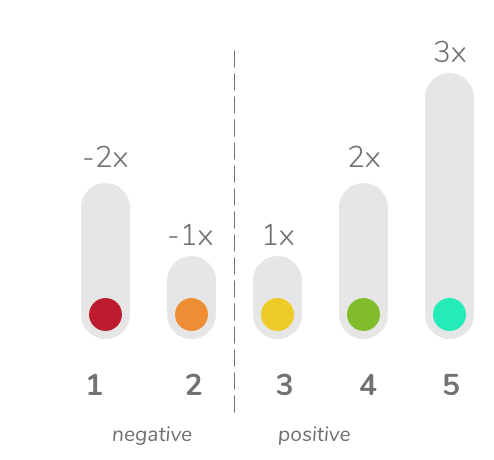
\includegraphics[scale=0.5]{images/ratings.png}
    \caption{Ratings}
    \label{fig:ratings}
\end{figure}
Questo porta l'utente ad esprimere valutazioni "estreme" (1/5 se negativa e 4/5 o 5/5 se positiva) solo per quei contenuti che ritiene veramente validi e valutazioni più moderate per i restanti.

Il numero di voti che un utente può esprimere giornalmente varia con il valore della sua influenza. E' stato infatti possibile osservare come questa determini la porzione di \textbf{Voting Power} che viene sottratta all'utente per uno specifico voto. Approssimativamente nel seguente modo:

\begin{itemize}
    \item \textbf{Nuovi Utenti:}
    \begin{itemize}
        \item 3/5 o 2/5 $\approx$ 20 voti
    \end{itemize}
    \begin{itemize}
        \item 4/5 o 1/5 $\approx$ 5 voti
    \end{itemize}
    \begin{itemize}
        \item 5/5 $\approx$ 2-3 voti
    \end{itemize}
    \item \textbf{Utenti Veterani (Influenza $\geq 90$):}
    \begin{itemize}
        \item 3/5 o 2/5 $\approx$ 40 voti
    \end{itemize}
    \begin{itemize}
        \item 4/5 o 1/5 $\approx$ 10 voti
    \end{itemize}
    \begin{itemize}
        \item 5/5 $\approx$ 4 voti
    \end{itemize}
\end{itemize}
% corretto commento di Andrea

Il voto espresso può successivamente essere modificato, con la variazione del rating espresso, o anche eliminato completamente. Nel primo caso verrà effettuato un aggiustamento della \textbf{Voting Power}, ridotta se il nuovo rating è più estremo del precedente, aumentata se meno estremo, nel secondo caso, la \textbf{Voting Power} viene completamente rimborsata. Da questo consegue la possibilità per gli utenti di cambiare le opinioni espresse nel tempo. Tuttavia alcuni utenti potrebbe abusare questa funzionalità eliminando o modificando propri voti per cui hanno già ricevuto le ricompense, per esempio relativi a post di Twitter sufficientemente vecchi e che quindi difficilmente riceveranno ulteriori voti, con lo scopo di ottenere un rimborso di Voting Power e poter quindi effettuare più voti nell'arco di una giornata. Il problema viene solo parzialmente arginato dal fatto che il numero di azioni che un utente può effettuare in una giornata è limitato. 
% corretto commento di Andrea

L'utente può inoltre scegliere tra tre categorie, prescelte dal sistema e che variano in base a piattaforma/tipo di contenuto, quella in cui esprimere la sua valutazione. Ciò non esclude che possa esprimere un voto sul medesimo contenuto in più di una categoria tra quelle disponibili. Attualmente esistono 12 categorie che elenchiamo:

\begin{multicols}{3}
    \begin{itemize}
        \item Like
        \item Smart
        \item Funny
        \item Chill
        \item Useful
        \item Knowledgeable
        \item Engaging
        \item Easy
        \item Interesting
        \item Affordable
        \item Beautiful
        \item Original
    \end{itemize}
\end{multicols}

Volendo fare alcuni esempi, nel caso di un post su Twitter o un video su Youtube abbiamo le categorie di \textbf{Like}, \textbf{Smart} e \textbf{Funny}, mentre per un NFT su Rarible, Foundation ecc. \textbf{Like}, \textbf{Original} e \textbf{Beautiful}.
\\
\\
Tramite l'utilizzo dell'explorer della blockchain ed effettuando noi stessi alcuni test di voto, è stato possibile eseguire una verifica delle categorie effettivamente esistenti nella piattaforma. Mentre nella documentazione ne trovavamo solamente 12, studiando le azioni di voto siamo riusciti ad individuarne 17, che elenchiamo:

\begin{multicols}{3}
    \begin{itemize}
        \item Popularity
        \item Intelligence
        \item Funny
        \item Chill
        \item Useful
        \item Knowledgeable
        \item Engaging
        \item Easy
        \item Interesting
        \item Affordable
        \item Beautiful
        \item Original
        \item Expensive
        \item Trustworthy
        \item Agreewith
        \item Wouldelect
        \item Fire
    \end{itemize}
\end{multicols}

Troviamo 5 categorie completamente nuove e 2 categorie che presentano una variazione del nome rispetto alla documentazione: \textbf{Popularity-Like} e \textbf{Intelligence-Smart}.
\\
\\
E' possibile esprimere un voto su qualsiasi cosa possieda un URL. Per questo motivo YUP viene definito come un sistema di valutazione di Internet, anche se la sua maggiore espressione è sul lato sociale. Nel caso delle piattaforme che supportano l'implementazione con l'estensione si può votare tramite l'\textbf{Overlay} (un'icona con il logo di YUP che appare alla base del contenuto). Per tutte le altre è sufficiente accedere all'estensione dal proprio browser. Una nuova funzionalità, implementata in data 22 Aprile 2021, permette, su siti integrati e non, di esprimere un voto con click destro sul contenuto interessato $\rightarrow$ Yup - The Opinion Layer of the Web $\rightarrow$ Like Page / Like Link per votare rispettivamente la piattaforma oppure il contenuto specifico.

\subsection{Collezioni}
La piattaforma permette, oltre all'espressione dei voti, anche la creazione di collezioni, paragonabili alle playlist di Spotify. Un utente può crearne un numero indefinito ed iniziare ad aggiungere a queste ultime i suoi post preferiti. Aggiungere un contenuto ad una collezione non costa Voting Power, ciò significa che tali operazioni possono essere effettuate anche quando l'utente ha esaurito la sua capacità di voto giornaliera. Al momento le ricompense creatore per le collezioni non sono implementate.

\subsection{Valore Sociale}

\begin{figure}[t]
    \centering
    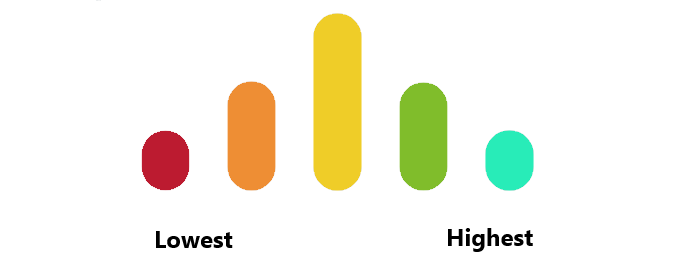
\includegraphics[scale=0.8]{images/colors.png}
    \caption{Colori del valore sociale}
    \label{fig:colours}
\end{figure}

Yup permette anche la visualizzazione del valore (sociale) di un contenuto, in base ai voti che ha ricevuto e a patto che sia stato votato almeno una volta, in relazione a tutti i contenuti che sono stati votati in una determinata categoria. Questo viene fatto tramite l'utilizzo di cinque colori in accordo con quelli dei cinque rating possibili.
\begin{itemize}
    \item \textbf{Verde:} top 20\%
    \item \textbf{Verde Giallastro:} 20\% - 40\%
    \item \textbf{Giallo:} 40\% - 60\%
    \item \textbf{Arancione:} 60\% - 80\%
    \item \textbf{Rosso:} 80\% - 100\%
\end{itemize}
I colori dei rating sono mostrati in Figura \ref{fig:colours}.

I voti negativi tendono a far diventare il colore di un contenuto più rosso e quelli positivi più verde. E' importante specificare come un contenuto potrebbe avere differenti colorazioni al variare della categoria. Per esempio, un tweet potrebbe aver ricevuto valutazioni estremamente positive per la categoria \textbf{Smart} ma valutazioni intermedie o negative per la categoria \textbf{Funny}.

\subsection{Integrazioni}
L'integrazione con l'estensione di YUP, intesa come la possibilità di esprimere un voto tramite l'\textbf{Overlay} piuttosto che l'estensione, è al momento disponibile solo su alcune piattaforme, principalmente riguardanti i Social Media:

\begin{itemize}
    \item \textbf{Twitter}
    \item \textbf{Youtube}
    \item \textbf{Reddit}
    \item \textbf{Google Maps}
\end{itemize}

Twitter costituisce un caso a parte poichè è attualmente l'unica piattaforma ad essere integrata anche tramite \textbf{OAuth}, ovvero è possibile registrarsi su Yup e verificare il proprio account tramite quello di Twitter.
Le prossime piattaforme per cui è programmata l'integrazione sono quelle relative al mercato di NFT quali \textbf{SuperRare}, \textbf{Audius} e \textbf{Rarible}. Al momento supportano comunque almeno l'\textbf{Action Tracking}, ovvero l'estensione registra i Like espressi su queste piattaforme e genera un corrispondente rating di 3/5 in categoria "Like", cosa che già avviene nelle piattaforme che supportano l'integrazione.

\section{Yup protocol}
Lo Yup Protocol è un protocollo di consenso sociale promosso ed incentivato da un'economia che si basa sulle opinioni degli utenti che fanno parte della rete, dove quest'ultima esiste all'interno del \textit{framework} del protocollo stesso.
Il protocollo facilita la misura, l'acquisizione e lo scambio di capitale sociale assicurando trasparenza e anonimità, anche se vedremo come quest'ultima non sempre sia garantita.
\\
Nello specifico il protocollo garantisce:
\begin{enumerate}
    \item \textit{Trasparenza}
    \item \textit{Monetizzazione equa e diretta} di contenuti e opinioni
    \item \textit{Identità digitali}
    \item \textit{Codici di condotta community-driven}
    \item \textit{Governance} basata sull'influenza
    \item \textit{Equa distribuzione} dei profitti pubblicitari
\end{enumerate}

Nelle sezioni successive vedremo come viene calcolato il peso che un utente e le sue azioni hanno all'interno della rete (\textbf{Influenza}), riservando opportuna attenzione anche a come sono definiti e calcolati i singoli parametri che contribuiscono a tale valore (\textbf{Age}, \textbf{Activity}, \textbf{Social Level} e \textbf{Boost}). Tratteremo inoltre alcuni aspetti tecnici del meccanismo delle ricompense e concluderemo con la trattazione dello strumento (\textbf{EOS-ETH Bridge} che permette a Yup di essere una piattaforma cross-chain e cross-platform.

\subsection{Influenza}
L'\textbf{Influenza} è una metrica, misurata nel range $0-100$, utilizzata come fondamento della \textit{governance} di rete ma anche per regolare la distribuzione dei token ricompensa.
Può essere definita come una rappresentazione del valore sociale di un utente: più alto è questo valore più peso avranno le sue opinioni. L'\textbf{Influenza} varia in base a quattro componenti che elenchiamo:

\begin{itemize}
    \item \textbf{Age (A)}
    \item \textbf{Activity (a)}
    \item \textbf{Social Level (s)}
    \item \textbf{Boost (b)}
\end{itemize}

Il suo valore è calcolato dal protocollo, per ogni utente, secondo l'equazione \ref{eq: influence_eq}:

\begin{equation}\label{eq: influence_eq}
    I = \beta\textsubscript{1}\sqrt{A} + \beta\textsubscript{2}\sqrt{a} + \beta\textsubscript{3}\sqrt{s} + b
\end{equation}

Dove i $\beta\textsubscript{i}$ sono delle costanti che nella documentazione non vengono specificate/spiegate. 
Di seguito, entreremo nel dettaglio dei singoli componenti: \textbf{Age}, \textbf{Activity}, \textbf{Social Level}, ed infine \textbf{Boost}.

\subsubsection{Age}
I token mantenuti da un account sono rappresentati dall'\textbf{Age} in un modo che si differenzia dal semplice \textit{staking - unstaking}. Infatti, oltre che considerare la quantità di token, viene tenuto in considerazione anche da quanto tempo l'utente ne è in possesso. Ne conseguono i seguenti vantaggi:
\begin{enumerate}
    \item Riflette l'impegno di un individuo all'interno della rete, impedendo che nuovi utenti possano incrementare in maniera significativa la propria influenza semplicemente comprando grandi quantità di token in un breve periodo
    \item Permette al protocollo di sostituire completamente il processo di \textit{staking - unstaking}, senza rinunciare a sicurezza a stabilità.
    \item Rende il tempo una vera e propria risorsa per gli utenti
\end{enumerate}

Definiamo questo parametro nell'equazione \ref{eq: age_eq}:

\begin{equation}\label{eq: age_eq}
    A = \sum\limits_{i=1}^nY\textsubscript{i}t\textsubscript{i}
\end{equation}

Dove $Y\textsubscript{i}$ rappresenta il \textit{token value} di una transazione che assegna dei token ad un utente e $t\textsubscript{i}$ il tempo trascorso dalla sua attuazione. 
\\
Notiamo come si dia importanza al tempo trascorso dal momento in cui un utente ottiene dei token.
% corretto commento di Andrea

\subsubsection{Activity}
L'\textbf{Activity} è una misurazione dell'attività e dell'impegno di un utente all'interno della rete. Per determinarla consideriamo i token YUP ottenuti dall'utente come ricompensa, sia essa per creazione o cura di contenuti, escludendo quindi quelli semplicemente acquistati. Esprimiamo l'Activity con l'equazione \ref{eq: activity_eq},

\begin{equation}\label{eq: activity_eq}
    a = \sum\limits_{i=1}^nR\textsubscript{u,i}
\end{equation}

dove $R\textsubscript{u,i}$ rappresenta le ricompense ricevute da uno specifico utente $u$ per un'azione $i$.
\\
E' importante notare come questo parametro non sia influenzato né dall'\textbf{Age} né dal bilancio dei token posseduti. In questo modo si evita che esso cambi nel momento in cui un utente trasferisce i token guadagnati. Inoltre per scoraggiare un'eccessiva attività priva di qualità col solo scopo di aumentare il valore  di activity, viene imposto un limite di 10 azioni giornaliere al conteggio dell'activity. Sarà ancora possibile effettuare delle azioni dopo le prime 10, tuttavia avranno un impatto nullo o marginale.

\subsubsection{Social Level}
Il \textbf{Social Level}, indicato con $\Bar{s}$ (\ref{eq: social_level_eq}), è un \textit{rank} numerico caratteristico di ogni account che viene determinato in base a tutti gli altri utenti (indirizzi) presenti nel network. Ogni account mantiene una lista, ordinata in un modo specifico che può modificare, di tutti gli altri utenti.
Definiamo questo parametro come segue,
% corretto commento di Andrea: [DOCUMENTAZIONE NON CHIARA, NON SIAMO SICURI DI QUESTO SOCIAL LEVEL]

\begin{equation}\label{eq: social_level_eq}
  \Bar{s} = \sum\limits_{i=1} \frac{s\textsubscript{i}*(\log (w\textsubscript{i}) + 1)}{\sqrt[5]{e\textsubscript{p}}}
\end{equation}

dove,
\begin{itemize}
    \item \textit{w (Weight)}: è un peso relativo ad un \textbf{ordine utente (UO)} ed è calcolato in base al livello dell'utente nell' \textbf{ordine aggregato (AO)} del blocco precedente (più qualche piccolo aggiustamento). Si veda Figura \ref{fig: social_table}.
    % corretto commento di Andrea [DA CHIEDERE: parte poco chiara su documentazione]
    \item \textit{e (Error)}: è una misura che dipende dalla relazione tra la lista mantenuta dall'utente e quella aggregata. Incentiva gli utenti ad effettuare un ordinamento corretto, poiché nel caso questo sia errato ne consegue una importante riduzione del loro livello sociale.
\end{itemize}

L'errore $e$ (\ref{eq: error_eq} viene espresso come la somma dei quadrati delle differenze tra il valore di ciascun elemento della lista $r$ e il corrispettivo \textit{rank} medio dell'account $\mu$,

\begin{equation}\label{eq: error_eq}
    e = \sum\limits_{i=1} (r\textsubscript{i} - \mu\textsubscript{i})^2
\end{equation}

Possiamo meglio comprendere il modo in cui funzionano i due diversi ordinamenti (AO e UO) tramite l'analisi delle Figura \ref{fig: social_table} e \ref{fig: social_simplified}.

\begin{figure}[h!]
    \centering
    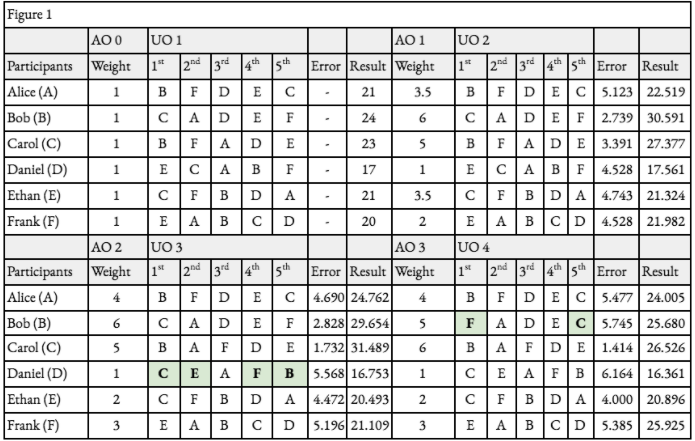
\includegraphics[width=\textwidth]{sociale_level}
    \caption{Ordinamento del Social Level}
    \label{fig: social_table}
\end{figure}

Alice (A), Bob (B), Carol (C), Daniel (D), Ethan (E), e Frank (F) sono i partecipanti di una rete con lo stesso protocollo di quello presentato. Questi utenti si elencano a vicenda nel "blocco di genesi" della piattaforma che utilizzano, dal più alto al più basso. Osserviamo i voti da loro espressi nei round 1, 2, 3, e 4 (UO) nella Figura \ref{fig: social_table}. Nel primo round il loro peso all'interno del network è uniforme mentre nel round 2 e nei successivi questo, e di conseguenza l'ordine, cambia.
Nel round 2 (UO 2) abbiamo i seguenti nuovi pesi per i sei account considerati: (A, 3.5), (B, 6), (C, 5), (D, 1) e i corrispondenti livelli sociali osservabili nella colonna \textit{Result} dell'immagine. Bob è quindi l'utente con più influenza e Daniel quello più basso. Nel round 3, Daniel tenta di incrementare l'influenza di Carol e decrementare quella di Bob mettendo la prima al vertice della sua lista ed i secondo in ultima posizione. Questo incrementa considerevolmente l'errore di Daniel (da 4.528 a 5.568) ma  fa andare con successo Carol al primo posto della lista (Carol UO 3 Result: 31.489), diventando prima in AO 3. Bob, con l'obiettivo di riprendersi la sua posizione, ordina Carol in ultima posizione nel round. Questo riduce la differenza tra Carol e Bob così come quella tra Carol e gli altri utenti. Tuttavia incrementa notevolmente l'errore di Bob (da 2.828 a 5.745) che fa diminuire il suo punteggio finale (Bob UO 4 Result: 25.680) e previene il suo tentativo di superare Carol.

\begin{figure}[h!]
    \centering
    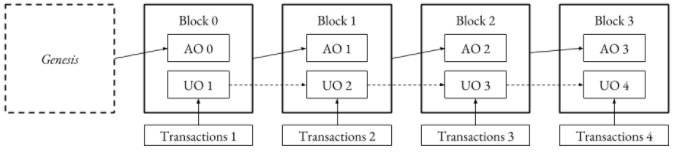
\includegraphics[width=\textwidth]{social_level_order}
    \caption{Ordinamento semplificato del Social Level}
    \label{fig: social_simplified}
\end{figure}


Se volessimo vedere quanto appena trattato in maniera più semplice possiamo osservare la Figura \ref{fig: social_simplified}. Osserviamo come l'ordine aggregato (AO) sia relativo ad ogni blocco e derivi da informazioni contenute nel blocco precedente, nello specifico dal blocco di genesi, in cui tutti i partecipanti hanno il medesimo peso, quando ci troviamo nella prima fase. L'ordine specifico di un utente (UO) invece, in assenza di transazioni che lo modifichino, rimane invariato tra un blocco e l'altro.

\subsubsection{Boost (Burning Mechanism)}
Con lo scopo di mantenere la fornitura di Yup tokens in distribuzione e aumentare la richiesta di questi ultimi, il protocollo fornisce un meccanismo definito come \textbf{Burning Mechanism}. Questo permette ad un account di "bruciare" permanentemente token posseduti per un temporaneo incremento della sua \textit{Influenza} (I) su una specifica azione da lui eseguita. Il numero di token che un account può investire con questo proposito è limitato.
Il \textbf{Boost} viene definito come nell'equazione \ref{eq: boost_eq},

\begin{equation}\label{eq: boost_eq}
    b = \sigma Y\textsubscript{burn,u}
\end{equation}

dove $\sigma$ è un \textbf{boost multiplier}.

\subsection{Meccanismo delle ricompense}
Il meccanismo di \textit{reward} dei token è una parte fondamentale del protocollo, in quanto si occupa della generazione di nuovi token e della loro successiva distribuzione. Esistono tre tipi di ricompense:

\begin{itemize}
    \item \textbf{Ricompense creatore} 
    \item \textbf{Ricompense curatore} 
    \item \textbf{Ricompense LQ:} destinate ai Liqiduity Provider
\end{itemize}

Gran parte dei token generati vengono distribuiti agli autori di contenuti in maniera proporzionale alle valutazioni che essi hanno ricevuto dalla \textit{community}. Questa frazione prende il nome di \textbf{creation allocation}. Tuttavia prima di darne una espressione in formule matematiche è necessario definire altri due elementi.
\\
\\
Nell'equazione \ref{eq: action_value} indichiamo con $V\textsubscript{h}$ il valore di una determinata azione che viene effettuata nella rete tramite l'interazione con il protocollo. Questa è espressa come il rapporto tra l'Influenza dell'azione e quella totale delle azioni eseguite sulla rete in un determinato periodo di tempo. Dove con Influenza di un'azione indichiamo semplicemente il valore I, precedentemente descritto, dell'utente che la effettua. 

\begin{equation}\label{eq: action_value}
    V\textsubscript{h} = \frac{I\textsubscript{i}}{I\textsubscript{i,t}} Y\textsubscript{c,t}
\end{equation}

Nell'equazione \ref{eq: content_value} indichiamo con $R\textsubscript{i}$, che prende il nome di \textbf{creation reward}, il valore in token di un contenuto, espresso come sommatoria dei valori delle azioni $V\textsubscript{j}$ eseguite per la creazione di quest'ultimo.

\begin{equation}\label{eq: content_value}
    R\textsubscript{i} = \sum\limits_{j=1}^m V\textsubscript{j}
\end{equation}


Adesso possiamo finalmente dare una definizione di \textbf{creation allocation} (\ref{eq: creation_allocation}). La definiamo, in relazione ad un determinato periodo di tempo $t$, come la sommatoria di tutte le corrispondenti \textbf{creation reward}.


\begin{equation}\label{eq: creation_allocation}
    Y\textsubscript{c,t} = \sum\limits_{i=1}^n R\textsubscript{i}
\end{equation}

\subsubsection{Ricompense Creatori e Curatori}
Definiamo la ricompensa di un \textbf{Creatore} $R\textsubscript{c}$ (\ref{eq: creator_reward}) come la porzione della ricompensa di un contenuto assegnata al creatore di quest'ultimo.
Sotto qualsiasi circostanza il creatore di un contenuto riceverà almeno il $50\%$ della ricompensa, mentre la parte rimanente viene divisa, in base all'influenza, tra il creatore e tutti i curatori che hanno contribuito al contenuto.
Definiamo $I\textsubscript{c}$ come l'influenza del creatore durante il periodo che intercorre dal momento della creazione e $I\textsubscript{pool,t}$ come la somma totale dell'Influenza di tutti i curatori che hanno votato il contenuto. In poche parole la porzione della seconda metà assegnata al creatore dipende dal rapporto tra la sua influenza e quella della \textit{pool}.
Possiamo ora esprimere $R\textsubscript{c}$ come,


\begin{equation}\label{eq: creator_reward}
    R\textsubscript{c} = R\textsubscript{i}\left(\frac{1 + \frac{I\textsubscript{c}}{I\textsubscript{pool,t}}}{2}\right)
\end{equation}
\\
\\
Ogni curatore riceve delle ricompense tenendo conto esclusivamente dei voti a loro successivi, i precedenti vengono pertanto ignorati. In questo modo si ricompensano maggiormente i curatori che hanno espresso una valutazione corretta sin da subito rispetto a coloro che arrivano in ritardo e che, in certi casi, potrebbero esprimere un'opinione condizionati dai voti già espressi. 
Definiamo la ricompensa di un \textbf{Curatore} $R\textsubscript{q}$ (\ref{eq: curator_reward}) come,

\begin{equation}\label{eq: curator_reward}
   R\textsubscript{q} = (\frac{1 - \frac{I\textsubscript{c}}{I\textsubscript{pool,t}}}{2}) \sum\limits_{j=1}^n (\frac{V\textsubscript{q}}{V\textsubscript{h,j}}) V\textsubscript{j}
\end{equation}


Dove $V\textsubscript{q}$ è il valore assegnato all'azione del curatore. $V\textsubscript{j}$ è un'azione $j$ a lui successiva mentre $V\textsubscript{h,j}$ rappresenta la somma dei valori delle azioni precedenti a $V\textsubscript{j}$.
\\
\\
Infine, indichiamo come ricompense LQ quelle destinate ad utenti che forniscono liquidità nella pool YUP-ETH di Uniswap. Queste sono proporzionali al numero di token YUP-ETH LQ messi in stake su \textit{Yup Racing}\footnote{https://www.yup.finance/}. Nella documentazione non vengono descritte formule relative al calcolo di quest'ultimo tipo di ricompense.
% corretto commento di Andrea [DA CHIEDERE: se devo spostare parte LQ qui]
% corretto commento di Andrea [DA CHIEDERE: Yup Racing non è citato prima perchè non sappiamo nulla se non che serva per lo stake di YUP-ETH]

\subsection{EOS-ETH Bridge}
Essendo Yup una piattaforma che si basa sull'utilizzo di due blockchain differenti, ne consegue la necessità di un meccanismo che permetta una interazione tra queste ultime. Questo ruolo viene ricoperto dallo \textbf{Yup Bridge}. La funzionalità è quella di rendere possibile il trasferimento di token tra le due blockchain. La modalità con cui i token vengono trasferiti tra le due blockchain prende il nome di \textbf{mint - burn}, i token non vengono effettivamente spostati bensì eliminati (burnt) su una blockchain e successivamente ne viene creato un quantitativo corrispondente sull'altra. Il servizio del \textbf{Bridge} è offerto da terzi e comporta per ogni spostamento di token il pagamento di una tassa, corrispondente ad una porzione degli YUP di cui si intende effettuare la migrazione. Il valore di questa tassa è direttamente correlato con il \textbf{gas} di Ethereum.

\section{Yup token}
Il token Yup è progettato per essere un \textit{crypto-asset} fruibile che permetta di creare un'economia sociale fondata sull'attività della \textit{community}. Esiste una versione del token sia su Ethereum che su EOS, il valore varia in base alla liquidità presente su quella specifica blockchain. 
Il token raggiunge i seguenti scopi:

\begin{itemize}
    \item \textbf{Incentivazione della partecipazione:} poichè utilizzati come ricompensa,
    \item \textbf{Governance:} in quanto utilizzato per governare il protocollo,
    \item \textbf{Incentivazione della liquidità:} i fornitori di liquidità ottengono Yup tokens come ricompensa,
\end{itemize}

Coloro che desiderano fornire liquidità per il protocollo devono aggiungere alla pool di Uniswap un volume equivalente di token ETH e token YUP. Per ottenere questi ultimi su Ethereum è sufficiente acquistarli in un exchange della blockchain oppure trasferire da EOS quelli guadagnati come ricompense curatore per l'utilizzo della piattaforma. Una volta inserita liquidità vengono ricompensati con dei token YUP-ETH Uniswap LP, questi ultimi attestano la loro percentuale di ownership della pool su Uniswap. Per concludere è necessario migrare questi ultimi su EOS e metterli in stake su Yup Racing. A questo punto si iniziano a ricevere token Yup, in proporzione alla liquidità fornita.
\\
\\
Nuovi token vengono creati secondo un programma prefissato per mezzo del \textit{token reward mechanicsm}, lo stesso meccanismo che si occupa anche della loro distribuzione.
\\
Il token di cui abbiamo appena parlato è stato introdotto nel protocollo una volta terminata la fase di \textbf{Beta testing} verso Settembre/Ottobre 2019. Precedentemente veniva utilizzato un altro token, indicato con \textbf{YUPX}, privo di valore il cui unico scopo era eseguire dei test sul corretto funzionamento del protocollo. Una volta conclusa la fase iniziale del progetto tutti gli utenti che vi avevano preso parte hanno ricevuto token YUP in rapporto 1 a 1 con i YUPX posseduti.

\section{Scopo del Tirocinio}
Le piattaforme Social Media basate su blockchain rappresentano oggi una valida alternativa alle soluzioni centralizzate, ed il meccanismo di reward risulta essere un ottimo metodo per incentivare la partecipazione degli utenti.
Lo scopo di questa tesi è far luce sul funzionamento della dApp di Yup, che risulta essere attualmente, una delle dApp sociali più utilizzate, con circa 6.000 utenti attivi al giorno\footnote{https://www.dapp.com/app/yup}. Ci siamo concentrati sulle possibili caratteristiche di un successo così importante, andando ad analizzare dettagliatamente il protocollo ed il meccanismo di reward, ed infine analizzando l'attività degli utenti. Nello specifico, abbiamo analizzato l'ambito sociale ed economico della piattaforma, quest'ultimo particolarmente importante nell'incentivare l'utilizzo della piattaforma stessa. Tra l'altro Yup si discosta proprio in questo ambito dalle numerose concorrenti anche solo per il valore del token che si riceve come ricompensa. Per esempio, durante \textit{Gennaio-Marzo 2021}, ha avuto un minimo di \textit{\euro1.28} ed un massimo di \textit{\euro5.85}. Se lo confrontiamo per esempio con i token utilizzati da social dApp concorrenti vediamo che: la moneta utilizzata su Hive, quindi da PeakD e Hive Blog, non ha mai superato nemmeno il valore di \textit{\euro1}, oppure quella utilizzata da Steemit, STEEM, solo recentemente, e per pochi giorni, ha superato il valore di \textit{\euro1}.


\subsection{Fase di studio}
\label{fasestudio_marker}
Nel protocollo di Yup sono presenti, in accordo con l'explorer utilizzato, 51 azioni differenti. Le elenchiamo di seguito suddivise per categoria e daremo una descrizione dettagliata esclusivamente di quelle più utilizzate e/o di cui è stato possibile comprenderne la funzionalità grazie al nome, al corpo JSON o tramite alcuni test effettuati durante la fase di analisi.

\begin{table}[t]
    \centering
    \caption{Azioni ambito \textbf{sociale}}
    \begin{tabular}{|l|l|l|l|}
    \hline
    $\bullet$ createcomv2 & $\bullet$ createvotev2 & $\bullet$ createvotev3 & $\bullet$ createvotev4 \\
    \hline
    $\bullet$ deletecom & $\bullet$ deletevote & $\bullet$ editacct & $\bullet$ editacct2 \\
    \hline
    $\bullet$ editvotev2 & $\bullet$ follow & $\bullet$ unfollow & $\bullet$ postvote \\
    \hline
    $\bullet$ postvotev2 & $\bullet$ postvotev3 & $\bullet$ postvotev4 \\
    \cline{1-3}
    \end{tabular}
    \label{tab: social_actions}
\end{table}

\begin{table}[t]
    \centering
    \caption{Azioni ambito \textbf{economico}}
    \begin{tabular}{|l|l|l|l|}
    \hline
    $\bullet$ claimcrrwds & $\bullet$ claimcurwds & $\bullet$ claimlqrwds2 & $\bullet$ stakelq \\
    \hline
    $\bullet$ unstakelq \\
    \cline{1-1}
    \end{tabular}
    \label{tab: economy_actions}
\end{table}
\clearpage

\begin{table}[t]
    \centering
    \caption{Azioni di \textbf{sistema}}
    \begin{tabular}{|l|l|l|l|}
    \hline
    $\bullet$ addblacklist & $\bullet$ addnblcklist & $\bullet$ createacct & $\bullet$ createcat \\
    \hline
    $\bullet$ getactivity & $\bullet$ getage & $\bullet$ getinfl & $\bullet$ getivlpool \\
    \hline
    $\bullet$ logacctv2 & $\bullet$ logactivity & $\bullet$ logage & $\bullet$ loggetage \\
    \hline
    $\bullet$ login & $\bullet$ loginfluence & $\bullet$ loguintval & $\bullet$ rmblacklist \\
    \hline
    \end{tabular}
    \label{tab: system_actions}
\end{table}

\begin{table}[t]
    \centering
    \caption{Azioni \textbf{sconosciute}}
    \begin{tabular}{|l|l|l|l|}
    \hline
    $\bullet$ claimtmrwds & $\bullet$ claimtrrwds & $\bullet$ delactusg & $\bullet$ dellqivls \\
    \hline
    $\bullet$ initvotecks & $\bullet$ logdouble & $\bullet$ logdoubleval & $\bullet$ noop \\
    \hline
    $\bullet$ processivlv3 & $\bullet$ processlqivl & $\bullet$ rmactusage & $\bullet$ setvotecks \\
    \hline
    $\bullet$ updatelstivl & $\bullet$ updlstlqivl & $\bullet$ vmcomp \\
    \cline{1-3}
    \end{tabular}
    \label{tab: unknown_actions}
\end{table}

\subsubsection{postvote}
L'azione di \textbf{postvote} (di cui possiamo trovare multiple versioni: postvote, postvotev2, postvotev3 e postvotev4) corrisponde alla votazione di un contenuto, non precedentemente valutato, da parte di un utente.
\\
Per l'esecuzione della azione sono necessari due attori e di conseguenza due chiavi private, quella di \textbf{yupcreators1} e dell'utente che ha espresso l'opinione. Troviamo queste informazioni nel campo \textbf{authorization} della postvote.
Le informazioni relative al voto sono invece presenti nel campo \textbf{data}. Elenchiamo le più importanti:

\begin{itemize}
    \item \textbf{caption:} link completo del contenuto votato
    \item \textbf{voter:} il nome EOS dell'account del votatore
    \item \textbf{category:} la categoria in cui è stato espresso il voto
    \item \textbf{like:} booleano settato 1 o 0, rispettivamente se il voto è positivo o negativo
    \item \textbf{rating:} un intero che indica l'intensità del voto in un range 1-3 se positivo e 1-2 se negativo
\end{itemize}

Ricordiamo quanto detto in Sezione \ref{voti_section}, ovvero che un voto viene misurato in una scala che va da 1/5 a 5/5. Le valutazioni 1/5 e 2/5 sono negative le restanti sono positive. Il modo in cui questi valori sono rappresentati con i parametri \textbf{like} e \textbf{rating} elencati sopra è il seguente: se like è settato a 0, quindi voto negativo, il campo rating potrà presentarsi con valore 1 o 2, rispettivamente l'equivalente di 1/5 e 2/5, se invece like è settato a 1, quindi voto positivo, potremo trovare nel campo rating il valore 1, 2 o 3, rispettivamente 3/5, 4/5 e 5/5.
\\
\\
L'unica differenza che è stato possibile osservare tra le varie versione di postvote è l'aggiunta di due parametri nel campo \textbf{data} nelle versioni v3 e v4:

\begin{itemize}
    \item \textbf{ram\_payer:} sempre yupcreators1
    \item \textbf{postid:} l'id con cui il contenuto viene salvato nel database di Yup
\end{itemize}

\subsubsection{createvote}
L'azione di \textbf{createvote} (di cui possiamo trovare le seguenti versioni: createvotev2, createvotev3 e createvotev4) corrisponde alla votazione di un contenuto già precedentemente valutato da un utente.
I campi in cui troviamo le informazioni relative alle autorizzazioni necessarie per la sua esecuzione e quelle relative al voto sono le stesse elencate precedentemente per la postvote. In questo caso troviamo, nel campo \textbf{authorization}, solo un attore che rappresenta l'utente. Questo vale solo per le versioni fino alla v3, infatti nel caso specifico della v4 compare anche un campo che indica anche yupcreators1 come attore.
\\
Per quanto riguarda le informazioni relative al voto, i parametri presenti nel campo \textbf{data} sono esattamente gli stessi che avevamo precedentemente elencato per postvote e postvotev2. L'unica differenza è che al posto del link del contenuto troviamo semplicemente l'id con cui è identificato nel database di Yup ("postid").

\subsubsection{claimcurwds}
L'azione di \textbf{claimcurwds} è relativa alla distribuzione delle ricompense per gli utenti in qualità di curatori. In questa sezione non discuteremo le claim di cui non siamo riusciti a comprendere la natura (\textbf{claimtmrwds} e \textbf{claimtrrwds}). Il corpo dell'azione presenta, nel campo \textbf{data}, un parametro che specifica il voteid, che permette di risalire anche al postid del contenuto, a cui fanno riferimento le ricompense assegnate. 
\\
Alcune variante della \textbf{claimcurwds} sono la \textbf{claimcrrwds} e la \textbf{claimlqrwds2}, rispettivamente relative alle ricompense creatori e a quelle LQ. La calimcrrwds ha come destinatario sempre yupcreators1 e contiene nel campo \textbf{data} il postid del contenuto creato. La claimlqrwds2 invece mantiene in tale campo semplicemente l'eosname dell'utente LQ a cui spettano le ricompense in questione.
\\
\\
Tramite lo studio effettuato sulla blockchain è stato possibile individuare ulteriori tipi di azioni che non erano presenti nella lista dell'explorer precedentemente mostrata. Elenchiamo queste ultime nella Tabella \ref{tab: appendix_actions} in Appendice A a pag. \pageref{appendix_marker}. Delle azioni mostrate in Appendice siamo riusciti a comprendere la funzionalità della \textbf{transfer}, la quale sembrerebbe propria di EOS per spostamenti di token e risorse.

\subsubsection{transfer}
Di seguito diamo una descrizione dei principali parametri individuati all'interno del campo \textbf{data} dell'azione in questione.

\begin{itemize}
    \item \textbf{from:} il mittente (yupyupyupyup nel caso di ricompense o il nome di un utente altrimenti)
    \item \textbf{to:} il nome EOS dell'utente
    \item \textbf{quantity:} il numero di token inviati
    \item \textbf{memo:} specifica la natura del trasferimento e presenta cinque possibilità: "Yup Creators Rewards", "Yup LQ Rewards", "Yup Extension Transfer", "Bridge Fee" e un indirizzo Ethereum. Rispettivamente sono relative a ricompense creatore, a ricompense liquity provider, al trasferimento utente-utente tramite l'estensione, al pagamento della tassa per il Bridge oppure al trasferimento su Ethereum dei propri token.
\end{itemize}

Durante le fase di studio del protocollo, abbiamo analizzato il meccanismo di ricompensa e gli Smart Contract utilizzati, focalizzandoci su quello principale (yupyupyupyup). 
Gli Smart Contract di Yup su EOS si differenziano, oltre a quello principale su cui ci siamo concentrati, da quelli relativi ai token, token.yup e lptoken.yup rispettivamente per il token ricompensa Yup ed il token YUP-ETH dei Liquidity Provider, a quelli relativi al servizio del Bridge, bridge.yup e lpbridge.yup rispettivamente per il Bridge relativo ai token Yup e per il Bridge relativo ai token YUP-ETH.
% commento Andrea [DA CHIEDERE: azioni/transazioni sono proprie di EOSIO più che di EOS, dove aggiungerne spiegazione]

Non tutte le azioni della lista sono state poi ritrovate nell'attività dello Smart Contract.
Pertanto, effettuando una intersezione ed un'unione dei due gruppi di azioni trovati, otteniamo i seguenti dati:

\begin{itemize}
    \item \textbf{AZIONI LISTA:} 51
    \item \textbf{AZIONI TROVATE:} 192
    \item \textbf{IN COMUNE:} 46
    \item \textbf{TOTALE:} 197
\end{itemize}

Pertanto abbiamo 5 azioni della lista che non sono state ritrovate nel protocollo: \textit{getactivity}, \textit{getage}, \textit{loggetage}, \textit{rmactusage} e \textit{vmcomp}. Dove le prime due iniziano ad essere utilizzate a partire dal \textit{21 Marzo 2021}, mentre le rimanenti non sono ancora mai state utilizzate. Abbiamo 146 azioni (Tabella \ref{tab: appendix_actions} in Appendice A a pag. \pageref{appendix_marker}) individuate durante la fase di analisi dei dati della blockchain che non vengono ritrovate nella lista dell'explorer.
\\
\\

\subsection{Fase di download}
Per scaricare i dati dalla blockchain è stato necessario recuperare i nomi dei vari Smart Contracts dalla documentazione di Yup e successivamente utilizzare l'endpoint \textit{Get Actions} delle API offerte da \textit{eosflare.io}, effettuando un numero di richieste in accordo con il limit rate imposto (\textit{100/Min}). E' stato invece possibile scaricare le informazioni relative agli account Yup esistenti grazie alle API (endpoint: \textit{/levels}) descritte nella documentazione.
Durante la fase di download, abbiamo collezionato le informazioni relative a tutte le azioni eseguite su Yup. Abbiamo poi recuperato le informazioni relative agli accounts registrati su Yup ed infine quelle relative ai singoli contributi sociali, ovvero i vari contenuti votati.
%I programmi utilizzati per fare quanto detto sopra sono stati realizzati in linguaggio Python. E' stata utilizzata una libreria esterna (\textit{ijson}) per gestire le elevate dimensioni del JSON risultate dal download dello storico di tutte le azioni.

\subsection{Fase di analisi}
Durante la fase di analisi ci siamo concentrati principalmente nell'analisi economica e sociale della piattaforma, andando a valutare l'attività degli utenti. In dettaglio, abbiamo osservato vari aspetti del protocollo, tra cui l'utilizzo delle varie azioni, l'attività in termini di utenza, le varie piattaforme sociali coinvolte, ecc. Nel Capitolo \ref{analisi_marker}, sono riportate tutte le analisi effettuate e le considerazioni sui risultati ottenuti.
%\\
%\\
%In base alle analisi effettuate abbiamo appurato l'esistenza di \textit{16.484} account Yup, di questi solo per \textit{10.914} è stato possibile ritrovare una corrispondente azione di creazione account nel protocollo. Considerando solo il periodo successivo alla conclusione della fase di Beta (\textit{6 Ottobre 2020 - Febbraio 2021}), risulta una media di circa \textit{700} utenti mensili socialmente attivi, ovvero che hanno effettuato almeno un'azione in ambito sociale in quel mese. Di questi è stato osservato un picco particolarmente alto nel mese di Settembre, specificamente tra il 23 e 24 del mese. Queste ultime considerazioni sono relative ai soli account non-Mirror, tuttavia nel capitolo dedicato alla fase di analisi tratteremo anche quelle che tengono in considerazione gli account di sistema.
%\\
%\\
%Restando in ambito sociale abbiamo individuato 1.884 piattaforme diverse che hanno ricevuto almeno un voto. Tra queste dominano tre delle quattro piattaforme integrate (in ordine Twitter, Youtube e Reddit), anche se è possibile notare una notevole presenza di quelle ad NFT. Vedremo come la maggior parte dei profili o gruppi votati all'interno di tali piattaforme trattino argomenti legati al mondo cripto.
%\\
%\\
%Spostandoci infine sull'ambito economico abbiamo analizzato il funzionamento del meccanismo di ricompense e la distribuzione dei token tra i vari utenti. Nel primo caso è stato notato come quelle destinate ai Creatori non vengano distribuite agli account Mirror corrispondenti bensì accumulate sull'account \textbf{yupcreators1}, apparentemente per una futura distribuzione quando più Creatori riscatteranno tali account o si iscriveranno alla piattaforma. Nel secondo è stato possibile osservare come gli utenti che hanno riscosso o possiedono più token siano, nella maggior pate dei casi, utenti che, oltre ad utilizzare il servizio, forniscono liquidità su Uniswap.
%\\
%\\
%\subsubsection{Introduzione ai grafici}
%Osserveremo nel dettaglio i risultati di questa fase nell'apposito capitolo (\textbf{Chapter 5: ANALISI}). Vedremo alcuni grafici, opportunamente commentati, che ci aiutano a comprendere i dati raccolti. Questi ultimi rappresentano in certi casi un'analisi della distribuzione dei dati in relazione a determinate categorie, ed in altri un'analisi temporale, sia essa effettuata su base mensile o giornaliera. In quasi tutti i casi effettueremo una distinzione tra account reali (non-Mirror) e di sistema (Mirror). Infine, nel caso specifico di analisi distributive, rappresenteremo solo una top 10 dei dati per motivi di ordine e comprensione, includeremo tutti quelli restanti nella categoria \textit{others}.


% CAPITOLO: IMPLEMENTAZIONE
\chapter{IMPLEMENTAZIONE}
\label{chapter_implementazione}
In questo Capitolo, presentiamo il codice prodotto durante la fase di download della blockchain e la fase di analisi. Principalmente, andremo ad analizzare quali sono stati gli strumenti e le librerie utilizzate.
Nella sezione successiva elencheremo gli strumenti che sono stati utilizzati per la fase di download: API ed endpoints, explorer della blockchain di EOS, linguaggi di programmazione e librerie esterne. Con l'obiettivo di rendere questa fase riproducibile in futuro riporteremo anche il codice dei programmi utilizzati sia per scaricare quei dati relativi al protocollo sia per scaricare quelli relativi agli utenti.

\section{Strumenti}
Siamo riusciti ad individuare il nome EOS del protocollo principale e di Smart Contracts secondari grazie all'elenco degli Smart Contracts presente sulla documentazione ufficiale di Yup. E' stato poi utilizzato \textbf{bloks.io} come explorer della blockchain\footnote{https://bloks.io/}, il quale permette la visualizzazione delle informazioni e dello storico azioni di uno specifico account/protocollo. Tramite il suo utilizzo è stato possibile condurre alcuni test, prima utilizzando l'estensione e poi osservando l'azione generata, atti ad indagare la funzionalità di alcune delle azioni presenti nel protocollo. \\
Abbiamo utilizzato le API di eosflare.io\footnote{eosflare.io/api} (URL: https://api.eosflare.io) per scaricare le azioni del protocollo dalla blockchain. Le richieste sono di tipo POST e gli endpoint disponibili i seguenti:

\begin{itemize}
    \item \textbf{[POST] Get Account:} informazioni relative ad un account EOS
    \item \textbf{[POST] Get Transaction:} informazioni relative ad una transazione
    \item \textbf{[POST] Get Actions:} permette il recupero delle azioni e relative informazioni
\end{itemize}

Il limit rate per le API sopracitate è di 100 richieste per minuto.
\\
\\
Abbiamo utilizzato le API ufficiali di Yup\footnote{https://docs.yup.io/protocol/yup-api} (URL: http://api.yup.io) per reperire informazioni relative agli utenti, tipo di account, token posseduti/guadagnati ecc., e per risalire al link di un contenuto votato quanto trovavamo un postid.
Le richieste sono di tipo GET e gli endpoint disponibili i seguenti:

\begin{itemize}
    \item \textbf{[GET] /levels:} JSON di tutti gli utenti Yup
    \item \textbf{[GET] /levels/users/{username}:} informazioni di uno specifico utente
    \item \textbf{[GET] /accounts/{username}:} informazioni di uno specifico utente
    \item \textbf{[GET] /followers/{username}:} seguaci di uno specifico utente
    \item \textbf{[GET] /following/{username}:} account seguiti da uno specifico utente
    \item \textbf{[GET] /accounts/actionusage/{eosname}:} azioni di voto effettuate da un utente
\end{itemize}

\begin{itemize}
    \item \textbf{[GET] /posts/post/{postid}/{voteid}:} informazione relative ad un voto/post
    \item \textbf{[GET] /comments/post/{postid}/{voteid}:} informazioni relativi ai commenti su un voto/post
    \item \textbf{[GET] /posts/interactions/{postid}/{voteid}:} informazioni relative alle interazioni su un voto/post
    \item \textbf{[GET] /votes/post/{postid}/voter/{username}:} informazioni relative ad un voto di uno specifico utente
\end{itemize}

I programmi utilizzati per effettuare le richieste alle API stati realizzati in linguaggio Python utilizzando la librearia \textit{requests} di Python3. Questi sono stati principalmente eseguiti su una macchina virtuale, utilizzando PowerShell come interfaccia, viste le elevate dimensione dei file JSON trattati (es. circa 33GB quello delle azioni).
Nelle sezioni successive li tratteremo nel dettaglio, includendo API ed endpoint utilizzati, e li differenzieremo in base alla funzione per cui sono stati realizzati.
\\
\\
%\subsection{Programma download dati (API, librerie}
L'analisi relativa allo Smart Contract di Yup è stata effettuata tramite l'utilizzo dell'endpoint Get\_Actions delle API di eosflare.io. L'endpoint richiede tre parametri: account\_name, pos e offset. Rispettivamente indicano il nome EOS dell'account, il numero di sequenza da usare come punto di partenza per l'analisi (per esempio 0|1: dalla più vecchia, -2: dalla più recente) e quante azioni recuperare (massimo 1000 per richiesta).
\\
In Listing \ref{action_example} mostriamo un esempio di un oggetto JSON che rappresenta una azione scaricata tramite tale metodo. Utilizzeremo i punti di sospensione in quei campi in cui i parametri variano in base al tipo di azione.

\begin{lstlisting}[language=json, label= {action_example}, captionpos=b, caption=Action JSON object]
{"actions":
    [{
        "global_action_seq":
        "account_action_seq":
        "block_num":
        "block_time":
        "irreversible":
        "action_trace": {
            "receipt": {
                "receiver": "yupyupyupyup"
                "global_sequence": 
                "code_sequence":
                "abi_sequence":
            },
            "act": {
                "account": ""
                "name": ""
                "authorization": [
                    {
                        "actor":
                        "permission":
                    }
                ],
                "data": {
                    ...
                },
                "hex_data":
            },
            "context_free":
            "elapsed":
            "except":
            "trx_id":
            "block_num":
            "block_time":
            "producer_block_id":
            "account_ram_deltas": [
                {
                    "account":
                    "delta":
                }
            ],
            "receiver": "yupyupyupyup",
            "inline_traces": []
        }
    }],
    "head_block_num":
    "last_irreversible_block":
}
\end{lstlisting}

I parametri del campo \textbf{data} variano a seconda del tipo di azione che prendiamo in considerazione. Abbiamo trattato i parametri specifici di alcune delle azioni più importanti in Sezione \ref{fasestudio_marker}.

In Listing \ref{actions_download} il programma utilizzato per scaricare e costruire il JSON mostrato in Listing \ref{action_example}. Sono necessari tre parametri in input. I primi due sono il corrispettivo dei primi due parametri dell'endpoint \textbf{Get Actions}, quindi nome dell'account e punto di partenza, mentre il terzo specifica il numero totale di azioni che vogliamo scaricare (multiplo di 1000). E' stato possibile individuare il nome EOS del protocollo di Yup grazie all'elenco degli Smart Contract presente nella loro documentazione ufficiale.

\begin{lstlisting}[language=Python, label={actions_download}, captionpos=b, caption=Actions Retrieval]
import requests, time, json, os.path, math

#API
EOSFLARE_API = "https://api.eosflare.io/v1/eosflare/get_actions"

#path
fileout = "/path/to/out/dir/"

# global values
max_per_minut = 100
tot           = 0

#funzione utility per inizializzare il JSON
def createJSON (response):
    response.pop("head_block_num")
    response.pop("last_irreversible_block")
    response = json.dumps(response)
    with open (fileout, "w") as outf:
        outf.write(response)
    outf.close()
    return

#funzione utility per l'append al JSON
def appendJSON (response):
    response = response["actions"]
    with open(fileout, mode="r+") as outf:
        outf.seek(os.stat(fileout).st_size - 2)
        for x in range(len(response)):
            outf.write( ", {}".format(json.dumps(response[x])))
        outf.write("]}")
    outf.close()

#funzione utility che effettua una singola richiesta API
def APIRequest (account_name, pos, offset):
    global tot
    data = {"account_name": account_name, "pos": int(pos), "offset": int(offset)}
    r = requests.post(EOSFLARE_API, json.dumps(data))
    status_code = r.status_code
    print("[", tot + 1, "]: ", status_code)

    while (status_code != 200):
        print(r.content)
        time.sleep(5)
        data = {"account_name": account_name, "pos": int(pos), "offset": int(offset)}
        r = requests.post(EOSFLARE_API, json.dumps(data))
        status_code = r.status_code
        print("[", tot + 1, "]: ", status_code)
    return r

#funzione utility per effettuare le richieste a blocchi da 100.000
def Get_Actions (account_name, start, n, ow):
    global offset, max_per_minut, tot
    offset, times, cont  = 1000, 0, 0
    pos = start
    
    while (times != n):
        print("TIME: ", times + 1)
        cont = 0
        # check per il limit rate
        while (cont != max_per_minut):
            r = APIRequest(account_name, pos, offset)

            r = r.json()
            if (pos == 1):
                createJSON(r)
            else:
                appendJSON(r)
                
            pos = pos + offset
            cont = cont + 1
            tot = tot + 1

        times = times + 1
        print("TOTAL: ", tot)
        if (times != n or ow != 0):
            print("SLEEPING")
            time.sleep(61)

    # se "end" non multiplo di 100.000
    if (ow > 0):
        print("ULTIMA POSIZIONE: ", pos - 1)
        start = pos
        max_per_minut = math.floor(ow / 1000)
        Get_Actions(account_name, start, 1, 0)
    return

def main():
    account_name, start, end = input("Account, start, end: ").split()
    start = int(start)
    end   = int(end)

    global fileout
    fileout = os.path.join(fileout, (account_name + ".json"))

    n_times = math.floor((end - (start-1)) / 100000) # numero blocchi da 100.000 azioni (100 richieste)
    ow      = (end - (start-1)) % 100000 # resto dopo ultimo blocco
    ow2     = (end - (start-1)) % 1000 # resto per ultima richiesta singola
    Get_Actions(account_name, start, n_times, ow)

    #se "end" non multiplo di 1.000
    if (ow2 > 0):
        start = (end - ow2) + 1
        r = APIRequest(account_name, start, ow2)
        r = r.json()
        try:
            appendJSON(r)
        except(FileNotFoundError):
            createJSON(r)



if __name__ == "__main__":
    main()
    print("|!|FINISHED|!|")
\end{lstlisting}


%subsection{Programma get postid}
Come accennano in precedenza, solo alcune azioni di voto (postvote|v2|v3|v4) contengono nel loro corpo il link dell'indirizzo trovato. Nel caso delle createvote troviamo un postid e per risalire tramite esso al contenuto in questione abbiamo utilizzato l'endpoint /posts/post/{postid} delle API ufficiali di Yup.


In Figura \ref{postid_example} e n Figura \ref{postid_download} mostriamo rispettivamente un esempio dell'oggetto JSON che rappresenta le informazioni di un post e un programma esempio che può essere utilizzato per effettuare tale operazione.

\begin{lstlisting}[language=json, label={postid_example} ,captionpos=b, caption=Postid JSON object]
{
    "__v": 0,
    "_id": {
        "postid": "9223372310339125417"
    },
    "author": "yupcreators1",
    "avatar": "",
    "caption": "https://twitter.com/binance/status/1400864050972606471",
    "catVotes": {
        "funny": {
            "down": 0,
            "up": 0
        },
        "intelligence": {
            "down": 0,
            "up": 0
        },
        "overall": {
            "down": 1,
            "up": 4
        },
        "popularity": {
            "down": 1,
            "up": 4
        }
    },
    "imgHash": null,
    "lastUpdated": "1622827004000",
    "onchain": true,
    "previewData": {
        "description": "\u201cHow to sell crypto on #Binance P2P using Lite mode. \n\n\u27a1\ufe0f https://t.co/grlK0QUGM5 https://t.co/fq7dOmVkDf\u201d",
        "favicons": [
            "https://abs.twimg.com/favicons/favicon.ico",
            "https://abs.twimg.com/icons/apple-touch-icon-192x192.png"
        ],
        "img": "https://pbs.twimg.com/profile_images/1377608897557585922/xKgTpvdh_400x400.jpg",
        "title": "Binance on Twitter",
        "url": "https://twitter.com/binance/status/1400864050972606471",
        "videos": []
    },
    "quantiles": {
        "affordable": "none",
        "agreewith": "none",
        "beautiful": "none",
        "chill": "none",
        "easy": "none",
        "engaging": "none",
        "expensive": "none",
        "funny": "none",
        "intelligence": "none",
        "interesting": "none",
        "knowledgeable": "none",
        "original": "none",
        "overall": "fourth",
        "popularity": "fourth",
        "trustworthy": "none",
        "useful": "none",
        "wouldelect": "none"
    },
    "rating": {
        "funny": {
            "ratingAvg": 0,
            "ratingCount": 0,
            "ratingSum": 0
        },
        "intelligence": {
            "ratingAvg": 0,
            "ratingCount": 0,
            "ratingSum": 0
        },
        "overall": {
            "ratingAvg": -0.2,
            "ratingCount": 5,
            "ratingSum": -1
        },
        "popularity": {
            "ratingAvg": -0.2,
            "ratingCount": 5,
            "ratingSum": -1
        }
    },
    "sextiles": {
        "affordable": "none",
        "agreewith": "none",
        "beautiful": "none",
        "chill": "none",
        "easy": "none",
        "engaging": "none",
        "expensive": "none",
        "funny": "none",
        "intelligence": "none",
        "interesting": "none",
        "knowledgeable": "none",
        "original": "none",
        "overall": "fourth",
        "popularity": "fourth",
        "trustworthy": "none",
        "useful": "none",
        "wouldelect": "none"
    },
    ...
}
\end{lstlisting}

\begin{lstlisting}[language=Python, label={postid_download} ,captionpos=b, caption=Postid Retrieval]
import requests, json


#API + endpoint
API = "http://api.yup.io/posts/post/"

def get_Postid(postid):
    url = API + str(postid)
    r = requests.get(url)
    r = r.json()
    print("POST CAPTION: ", r["caption"])
    return



def main():
    postid = input("POSTID: ")
    get_Postid(postid)


if __name__ == "__main__":
    main()
    print("|!|DONE|!|")
\end{lstlisting}

Se si partisse da un JSON contenente tutte le azioni da analizzare, come nel nostro caso, basta effettuare il parsing del JSON e considerare solo le azioni di createvote, estrapolare il parametro \textit{postid} nel campo \textit{data} e passarlo alla funzione \textbf{get\_Postid} appena descritta.
\\
\\
%\subsection{Programma download JSON utenti (API, librerie}
I dati relativi a tutti gli account/utenti presenti sul servizio sono stati reperiti utilizzando l'endpoint /levels delle API ufficiali.
\\
\\
Di seguito troviamo in Figura \ref{user_example} un esempio dell'oggetto JSON che rappresenta un utente e in Figura \ref{users_download} il programma utilizzato per il download di tutti gli utenti.

\begin{lstlisting}[language=json, label={user_example}, captionpos=b, caption=User JSON object]
{
    "__v": 0,
    "_id": 
    "avatar": 
    "balance": {
        "EOS": 
        "YUP": 
        "YUPETH":
        "YUPX":
    },
    "bio": 
    "claimed_creator_rewards": 
    "cum_deposit_time":,
    "eosname": 
    "fullname": 
    "last_interval_claimed": 
    "skey":
    "total_claimed_rewards": 
    "total_creator_rewards":
    "total_stake": {
        "YUPETH": 
    },
    "total_vote_value": 
    "twitterInfo": {
        "isAuthUser": 
        "isMirror": 
        "isTracked": 
        "userId": ,
        "username": 
    },
    "username": 
    "weight": # Influenza
}
\end{lstlisting}

\begin{lstlisting}[language=Python, label={users_download} ,captionpos=b, caption=Users Retrieval]
import requests, json

#API
YUP_API = "http://api.yup.io/levels"
#output path
outpath = "/pato/to/out/dir/"


def printUsers (response):
    cont = 0
    for el in response:
        if (el["_id"]): 
            cont = cont + 1
    print("N_USERS: ", cont)
    return


def writeJSON(name, response):
    filename = outpath + name + ".json"
    with open(filename, "w") as outf:
        outf.write(response)
    outf.close()
    return


def main():
    r = requests.get(YUP_API)
    print(r.status_code)

    # display number of users found
    r = r.json()
    printUsers(r)

    # generate JSON
    r = json.dumps(r)
    writeJSON("yup_accounts", r)


if __name__ == "__main__":
    main()
    print("|!|DONE|!|")
\end{lstlisting}


% CAPITOLO: ANALISI
\chapter{ANALISI}
\label{analisi_marker}
In questo Capitolo presentiamo le analisi effettuate sulla piattaforma Yup. In dettaglio, elencheremo i dati che sono stati raccolti ed i corrispondenti risultati. Effettueremo un'analisi degli utenti e della loro attività all'interno della piattaforma, concentrandoci sulla distribuzione delle azioni di creazione account e di quelle di voto su base mensile. In particolare, considerando queste ultime, daremo una rappresentazione delle principali piattaforme coinvolte.
Successivamente ci sposteremo su analisi volte ad indagare l'aspetto economico di Yup, di fatto ci concentreremo sulla distribuzione dei token tra i vari utenti e sull'utilizzo del Bridge.
Con l'obiettivo di facilitarne comprensione e lettura li rappresenteremo tramite l'utilizzo di tabelle e grafici di vario tipo. Concluderemo con dei grafici che ripetono alcune analisi precedenti però su base giornaliera.

\section{Dataset}
Il dataset raccolto nella prima fase del lavoro contiene tutte le azioni presenti sullo smart contract principale (\textbf{yupyupyupyup}) dal \textit{15 Settembre 2018}, periodo di inizio della sua attività, fino al \textit{28 Febbraio 2021}. In questo lasso di tempo sono state effettuate un numero di azioni/interazioni con il protocollo pari a $23.567.430$. Sono anche state scaricate le azioni degli account e smart contract secondari, nonostante non sia stata effettuata nessuna analisi su questi poiché le azioni presenti sono ripetizioni di quelle dello smart contract principale.


Per completezza riportiamo comunque anche il numero di azioni relative agli smart contract secondari, insieme alla loro data di inizio attività, in quanto differisce da quella di \textbf{yupyupyupyup}.

\begin{itemize}
    \item \textbf{yupaccounts1:} 1.801.246 (data inizio: \textit{24 Giugno 2019})
    \item \textbf{token.yup:} 354.187 (data inizio: \textit{9 Ottobre 2020})
    \item \textbf{lptoken.yup} 506 (data inizio: \textit{13 Ottobre 2020})
    \item \textbf{bridge.yup} 369.181 (data inizio: \textit{10 Ottobre 2020}
    \item \textbf{lpbridge.yup} 291.902 (data inizio: \textit{5 Novembre 2020})
\end{itemize}

In Figura \ref{fig:actionsDistribution} mostriamo una rappresentazione della distribuzione dei vari tipi di azioni (192) effettuate dal protocollo, mentre in Figura \ref{fig:actionsMensile} osserviamo un'analisi dell'attività del protocollo su base mensile.

\begin{figure}[h!]
    \centering
    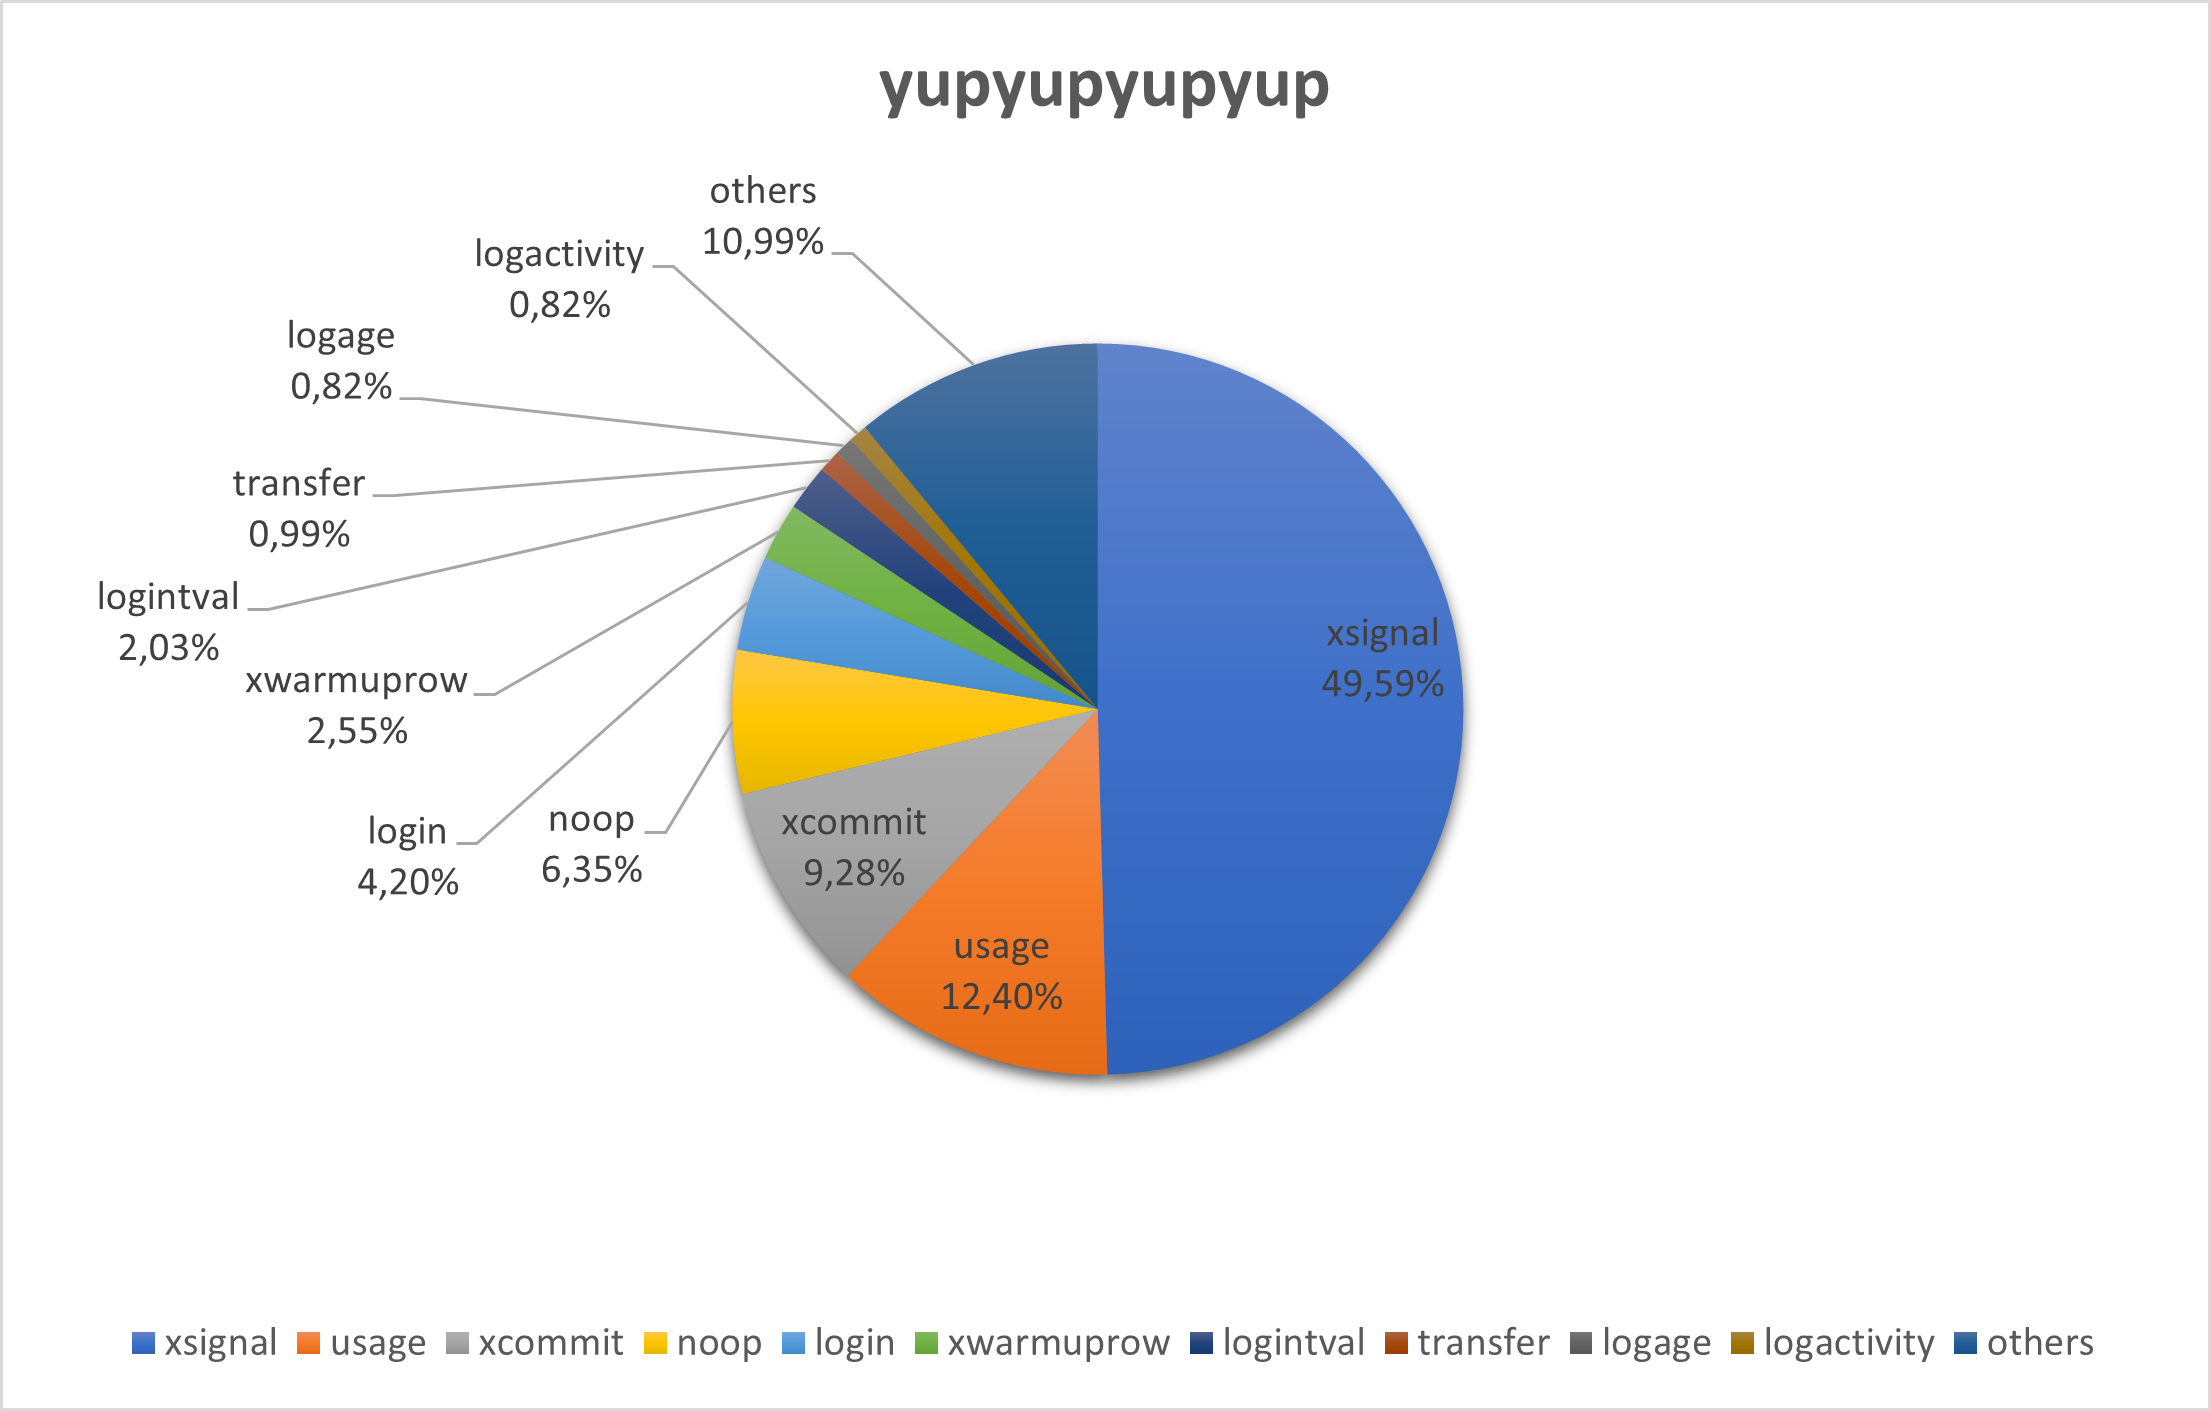
\includegraphics[width=1\textwidth]{graphs/torta_azioni.png}
    \caption{Rappresenta la distribuzione dei vari tipi di azioni, in \textbf{others} sono incluse tutte le azioni non presenti in top 10}
    \label{fig:actionsDistribution}
\end{figure}

In Figura \ref{fig:actionsDistribution} osserviamo come le tre azioni più utilizzate (\textit{xsignal}, \textit{usage} e \textit{xcommit}) facciano parte di quelle azioni non ritrovate nella lista dell'explorer (Tabella \ref{tab: unknown_actions} a Pagina \pageref{tab: unknown_actions}), dove la \textit{xsignal} ricopre quasi il 50\% delle azioni effettuate sul protocollo. Purtroppo non è stato possibile determinare con certezza la funzione di queste ultime, ma si suppone siano delle azioni proprie di EOS.IO relative alla gestione degli Smart Contract.
Un altro punto interessante di questa analisi consiste nell'aver individuato una buona presenza dell'azione \textit{noop} (no operation). Questa viene ripetuta un numero di volte considerevole (\textit{1.496.047}) se si considera che apparentemente non abbia alcun scopo, come dimostrato dal fatto che il campo \textit{data} del JSON che la caratterizza è completamente vuoto. Ciononostante, è importante notare che l'esecuzione di questa operazioni consumi comunque risorse, anche se non ha nessun effetto concreto.

\begin{figure}[h!]
    \centering
    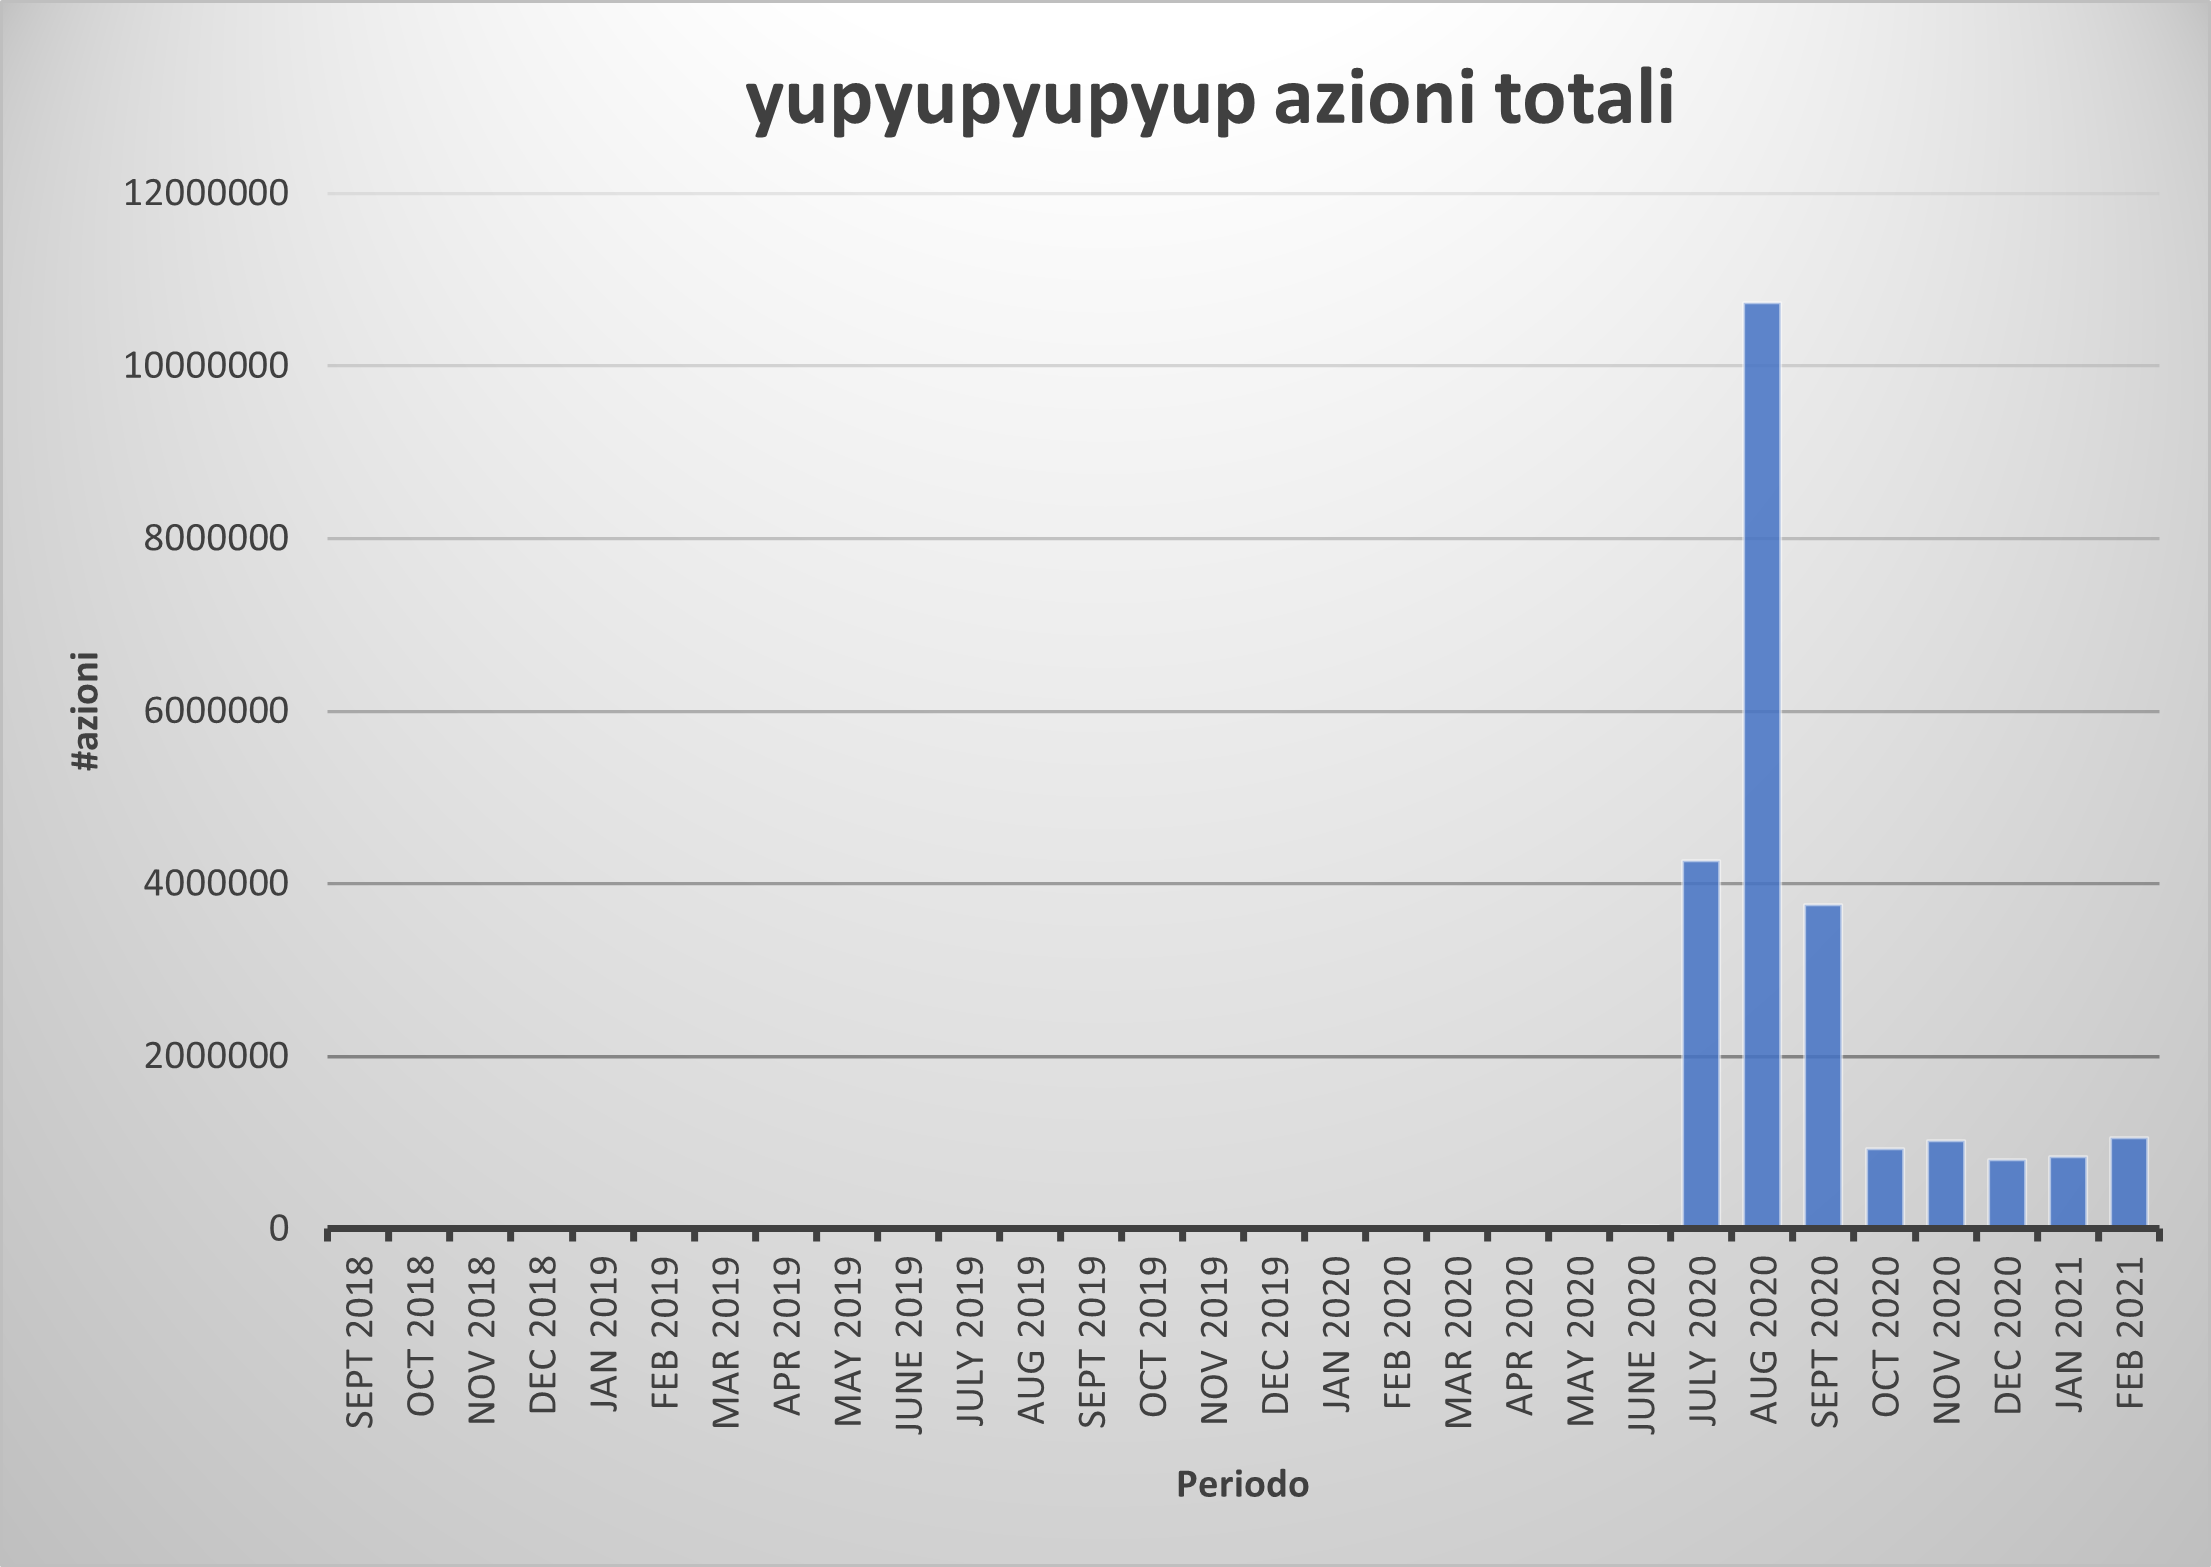
\includegraphics[width=1\textwidth]{graphs/mensile_azioni.png}
    \caption{Rappresenta la distribuzione delle azioni su base mensile, senza distinzione dei tipi, in modo da individuare particolari picchi di attività.}
    \label{fig:actionsMensile}
\end{figure}

In Figura \ref{fig:actionsMensile} possiamo constatare come l'attività del protocollo fino al mese di Giugno 2020 sia pressoché insignificante se paragonata ai mesi successivi. Abbiamo un particolare picco di attività nel periodo di Agosto 2020 ed è molto interessante come questo sia causato quasi esclusivamente da sole 4 azioni: \textbf{xsignal (6.805.319)}, \textbf{usage (1.701.330)}, \textbf{xcommit (1.293.877)} e \textbf{xwarmuprow (330.829)}. Queste costituiscono infatti più del 94\% dell'attività in quel mese. Purtroppo non è individuato alcun motivo che possa motivare un tale incremento in attività. E' tuttavia possibile che la ragione sia legata alla preparazione al passaggio tra la fase Beta di Yup e quella finale, entrata in funzione il \textit{6 Ottobre 2020}. 

\section{Utenza}
I dati relativi agli utenti Yup sono stati reperiti in due modalità: conteggiando il numero di \textbf{createacct} sullo smart contract e scaricando il JSON contente tutti gli utenti dalle API ufficiali.
Tuttavia, il numero di utenti ottenuti tramite API ufficiali non coincide con il numero di createacct, il che ci porta a pensare che alcuni utenti siano stati registrati senza l'interazione con il protocollo.
Per chiarezza, definiamo \textit{Creati} gli account per i quali esiste un'azione createacct, e \textit{non-Creati} gli altri account ottenuti dalle API, ma per i quali non esiste l'azione createacct.
%Come vedremo a breve il numero di account presenti nel JSON è notevolmente superiore al numero di createacct, ciò significa che esistono account non generati tramite l'interazione con il protocollo.

In Tabella \ref{table:usersClassification} mostriamo il numero degli utenti reperiti.

\begin{table}[h!]
\centering
\begin{tabular}{ |c|c|c|c|c|c| }
 \hline
 \textbf{Totale} & non-Creati & Creati & Mirror & non-Mirror\\
 \hline
 \textbf{16.484} & 5.439 & 11.045 & 7.607 & 3.438\\
 \hline
\end{tabular}
\caption{Classificazione dei tipi di account a Febbraio 2021}
\label{table:usersClassification}
\end{table}

La tabella mostra che il numero di account non-creati è circa la metà di quelli creati, e tra quelli creati una larga parte sono account mirror.
Poco meno di un terzo degli account creati sono non-Mirror e di questi meno della metà (un decimo del totale) hanno collegato il loro account Twitter all'account Yup.
In totale ci sono 7.607 Mirror e 8.877 non-Mirror.

In Figura \ref{fig:usersClassification2}, considerando solo gli account non-Mirror, proponiamo un confronto tra la distribuzione di account linkati a Twitter e non (registrati tramite e-mail o WalletConnect).

\begin{figure}[t]
    \centering
    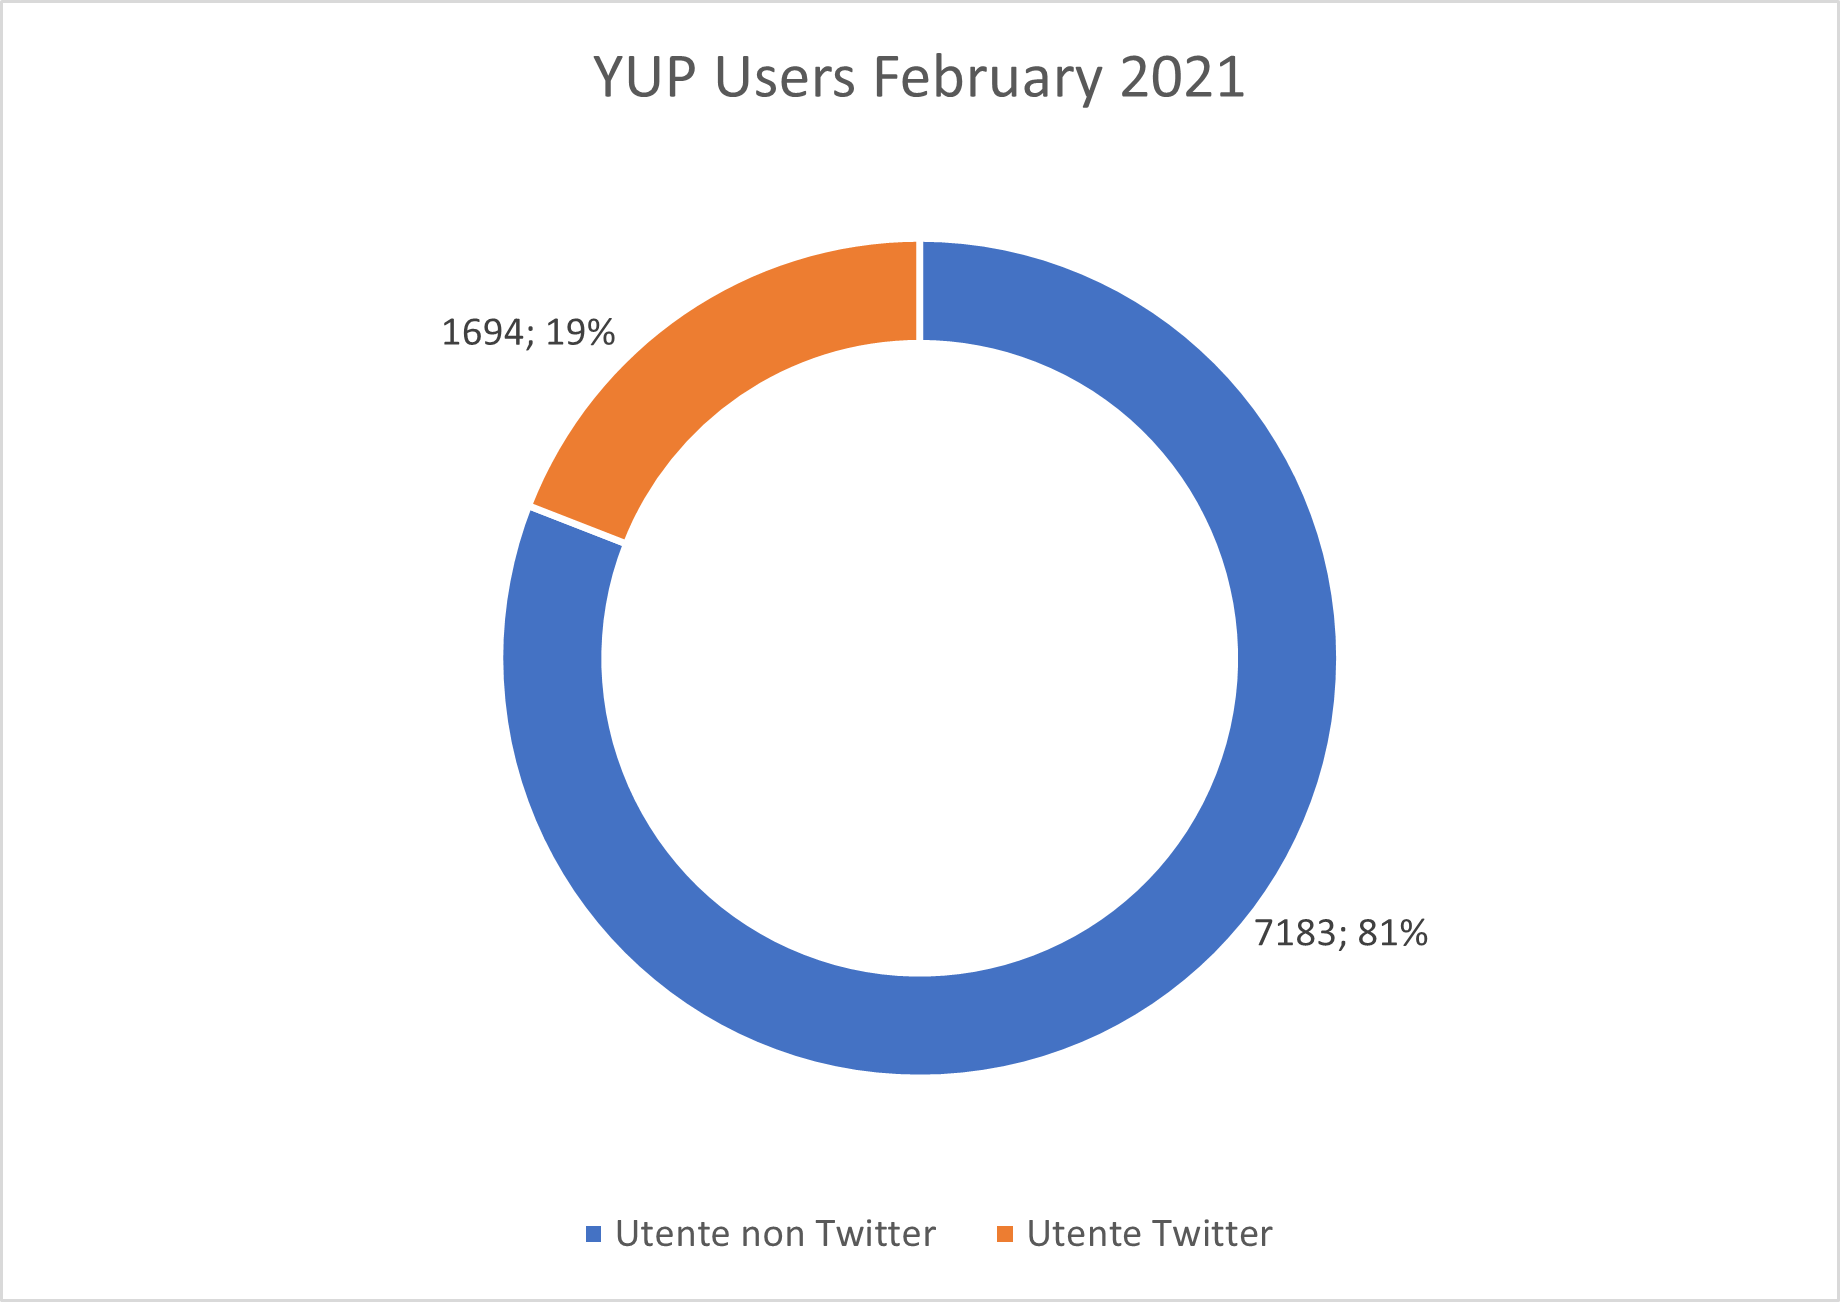
\includegraphics[width=0.8\textwidth]{graphs/users_feb.png}
    \caption{Tipi di utenti Febbraio 2021}
    \label{fig:usersClassification2}
\end{figure}

Dalla Figura è facile accorgersi come, almeno al momento, la maggior parte degli utenti Yup non si sia registrata alla piattaforma mediante il proprio account Twitter oppure semplicemente non abbia effettuato il linking una volta registrato tramite Email o Wallet Connect.
Questo potrebbe essere legato al fatto che la piattaforma non è ancora ben conosciuta al mondo social, nonostante la sua integrazione, o che gli utenti a cui si rivolge sono perlopiù legati o familiari con il mondo delle criptovalute.


Essendo presente, nel caso di alcuni account, questo collegamento tra Yup e Twitter, siamo andati a vedere che relazione ci fosse tra le relazioni di follow tra gli utenti sulle due piattaforme. Sono stati tenuti in considerazione solo i follower di account Yup collegati a Twitter, altrimenti non sarebbe stato possibile effettuare la verifica. Mostriamo in Figura \ref{fig:followersComparison} le relazioni di follow presenti solo su Yup (in blu) e quelle presenti sia su Yup che su Twitter (in arancione).

\begin{figure}[t]
    \centering
    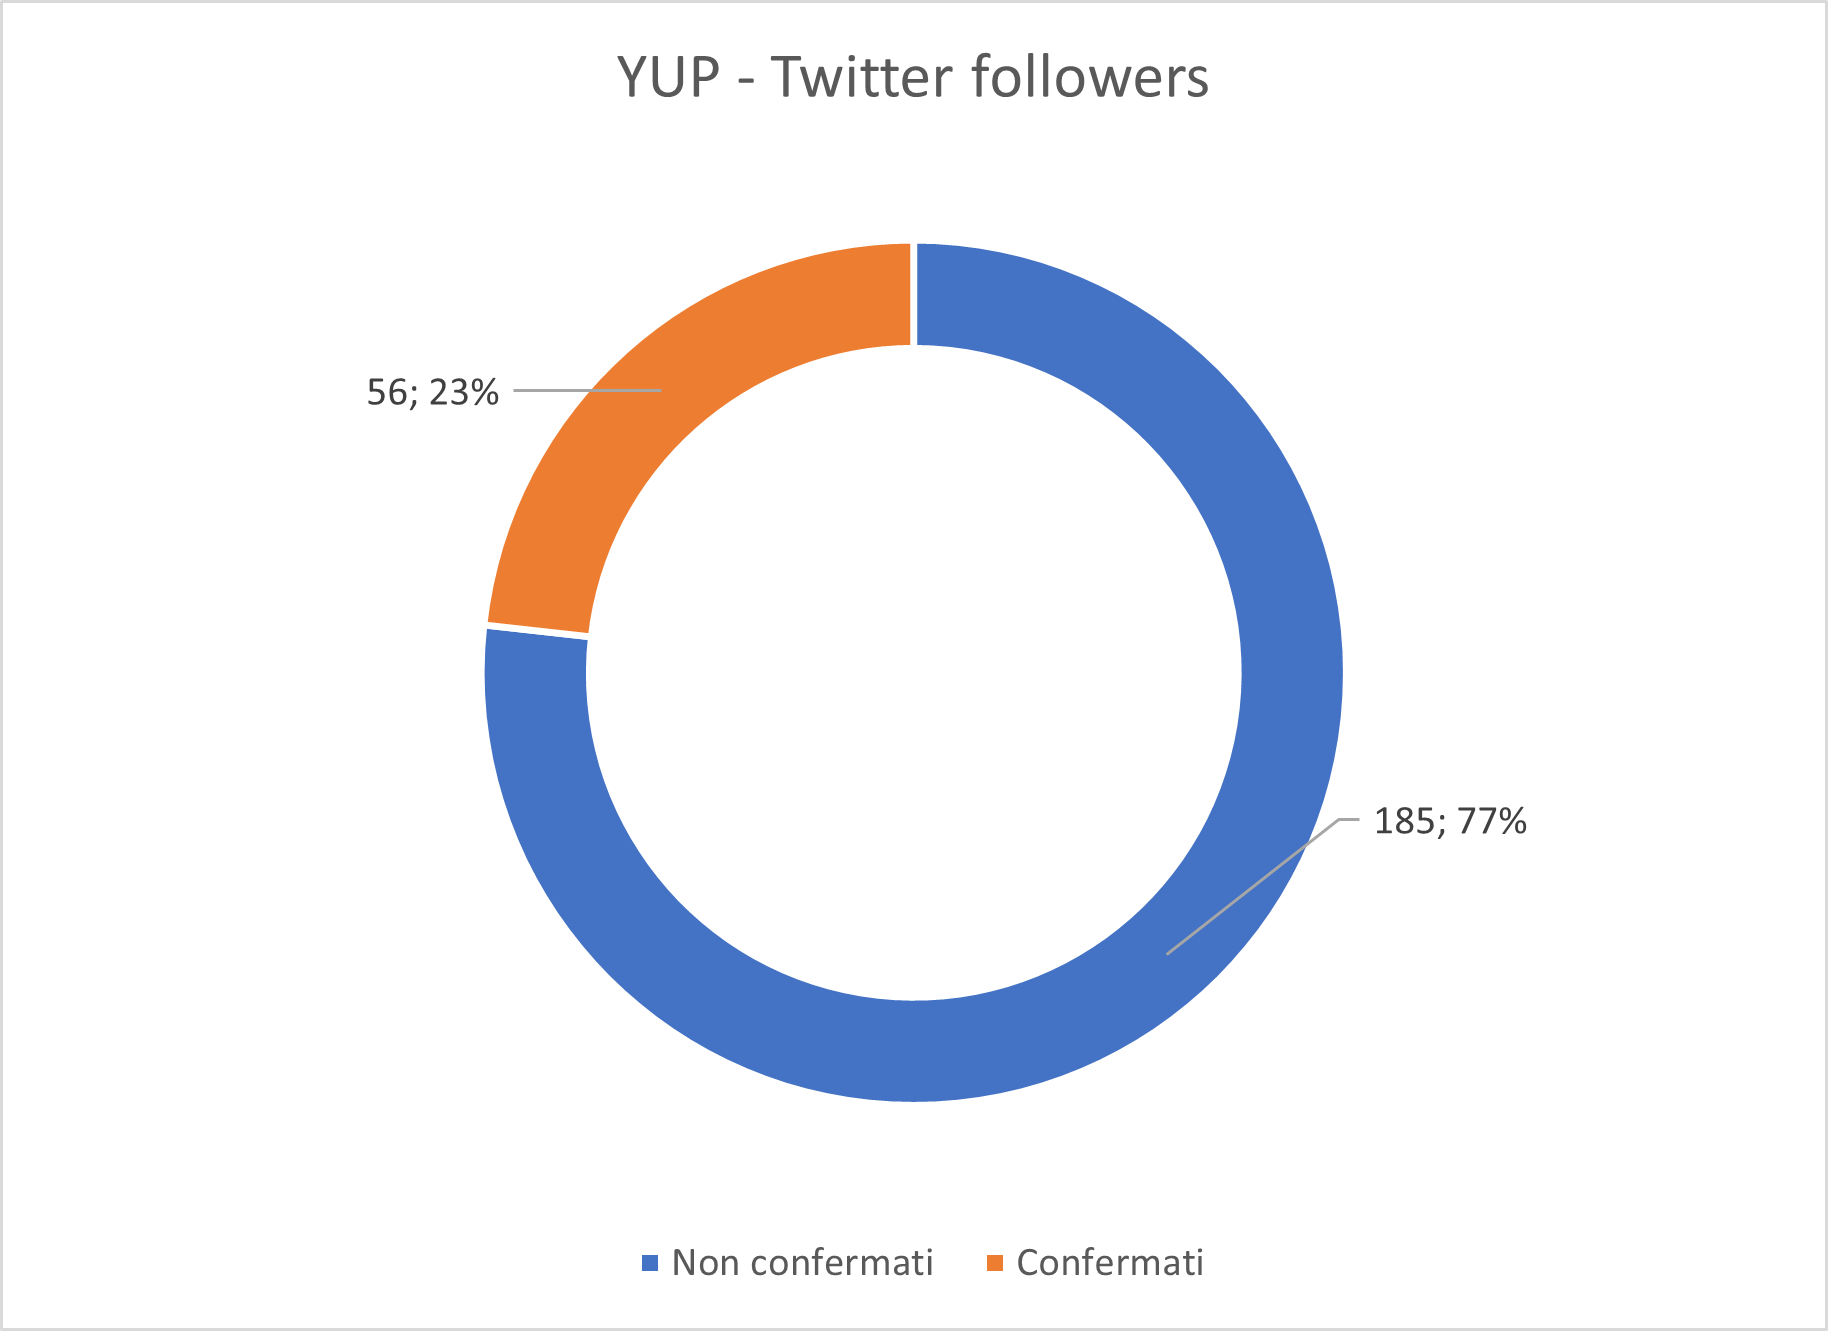
\includegraphics[width=0.8\textwidth]{graphs/followers.png}
    \caption{Follower confermati, segue su Yup e segue anche su Twitter, e quelli non confermati, non segue su Twitter.}
    \label{fig:followersComparison}
\end{figure}

Questa analisi ci permette di affermare che, almeno tra gli utenti Yup con un account Twitter collegato, la funzionalità di following sulla piattaforma viene raramente utilizzata, infatti troviamo solo 241 follow espressi da su quasi 1.700 utenti. Oltretutto in oltre 3/4 dei casi, l'utente che segue lo fa solamente su Yup.
Questi risultato mette in luce il fatto che il follow su Yup non tende ad avere funzioni sociali come su Twitter.

\subsection{Createacct}
Anche per le azioni di creazione account (createacct) è stata effettuata un'analisi temporale su base mensile. In questo modo ci è possibile apprendere quali siano stati i mesi chiave che hanno visto un maggiore di utenti registrati sulla piattaforma. Mostriamo in Figura \ref{fig:createacctMensile_conmirr} e \ref{fig:createacctMensile_nomirr} il numero di createacct per mese, rispettivamente includendo ed escludendo account Mirror.

\begin{figure}[t]
    \centering
    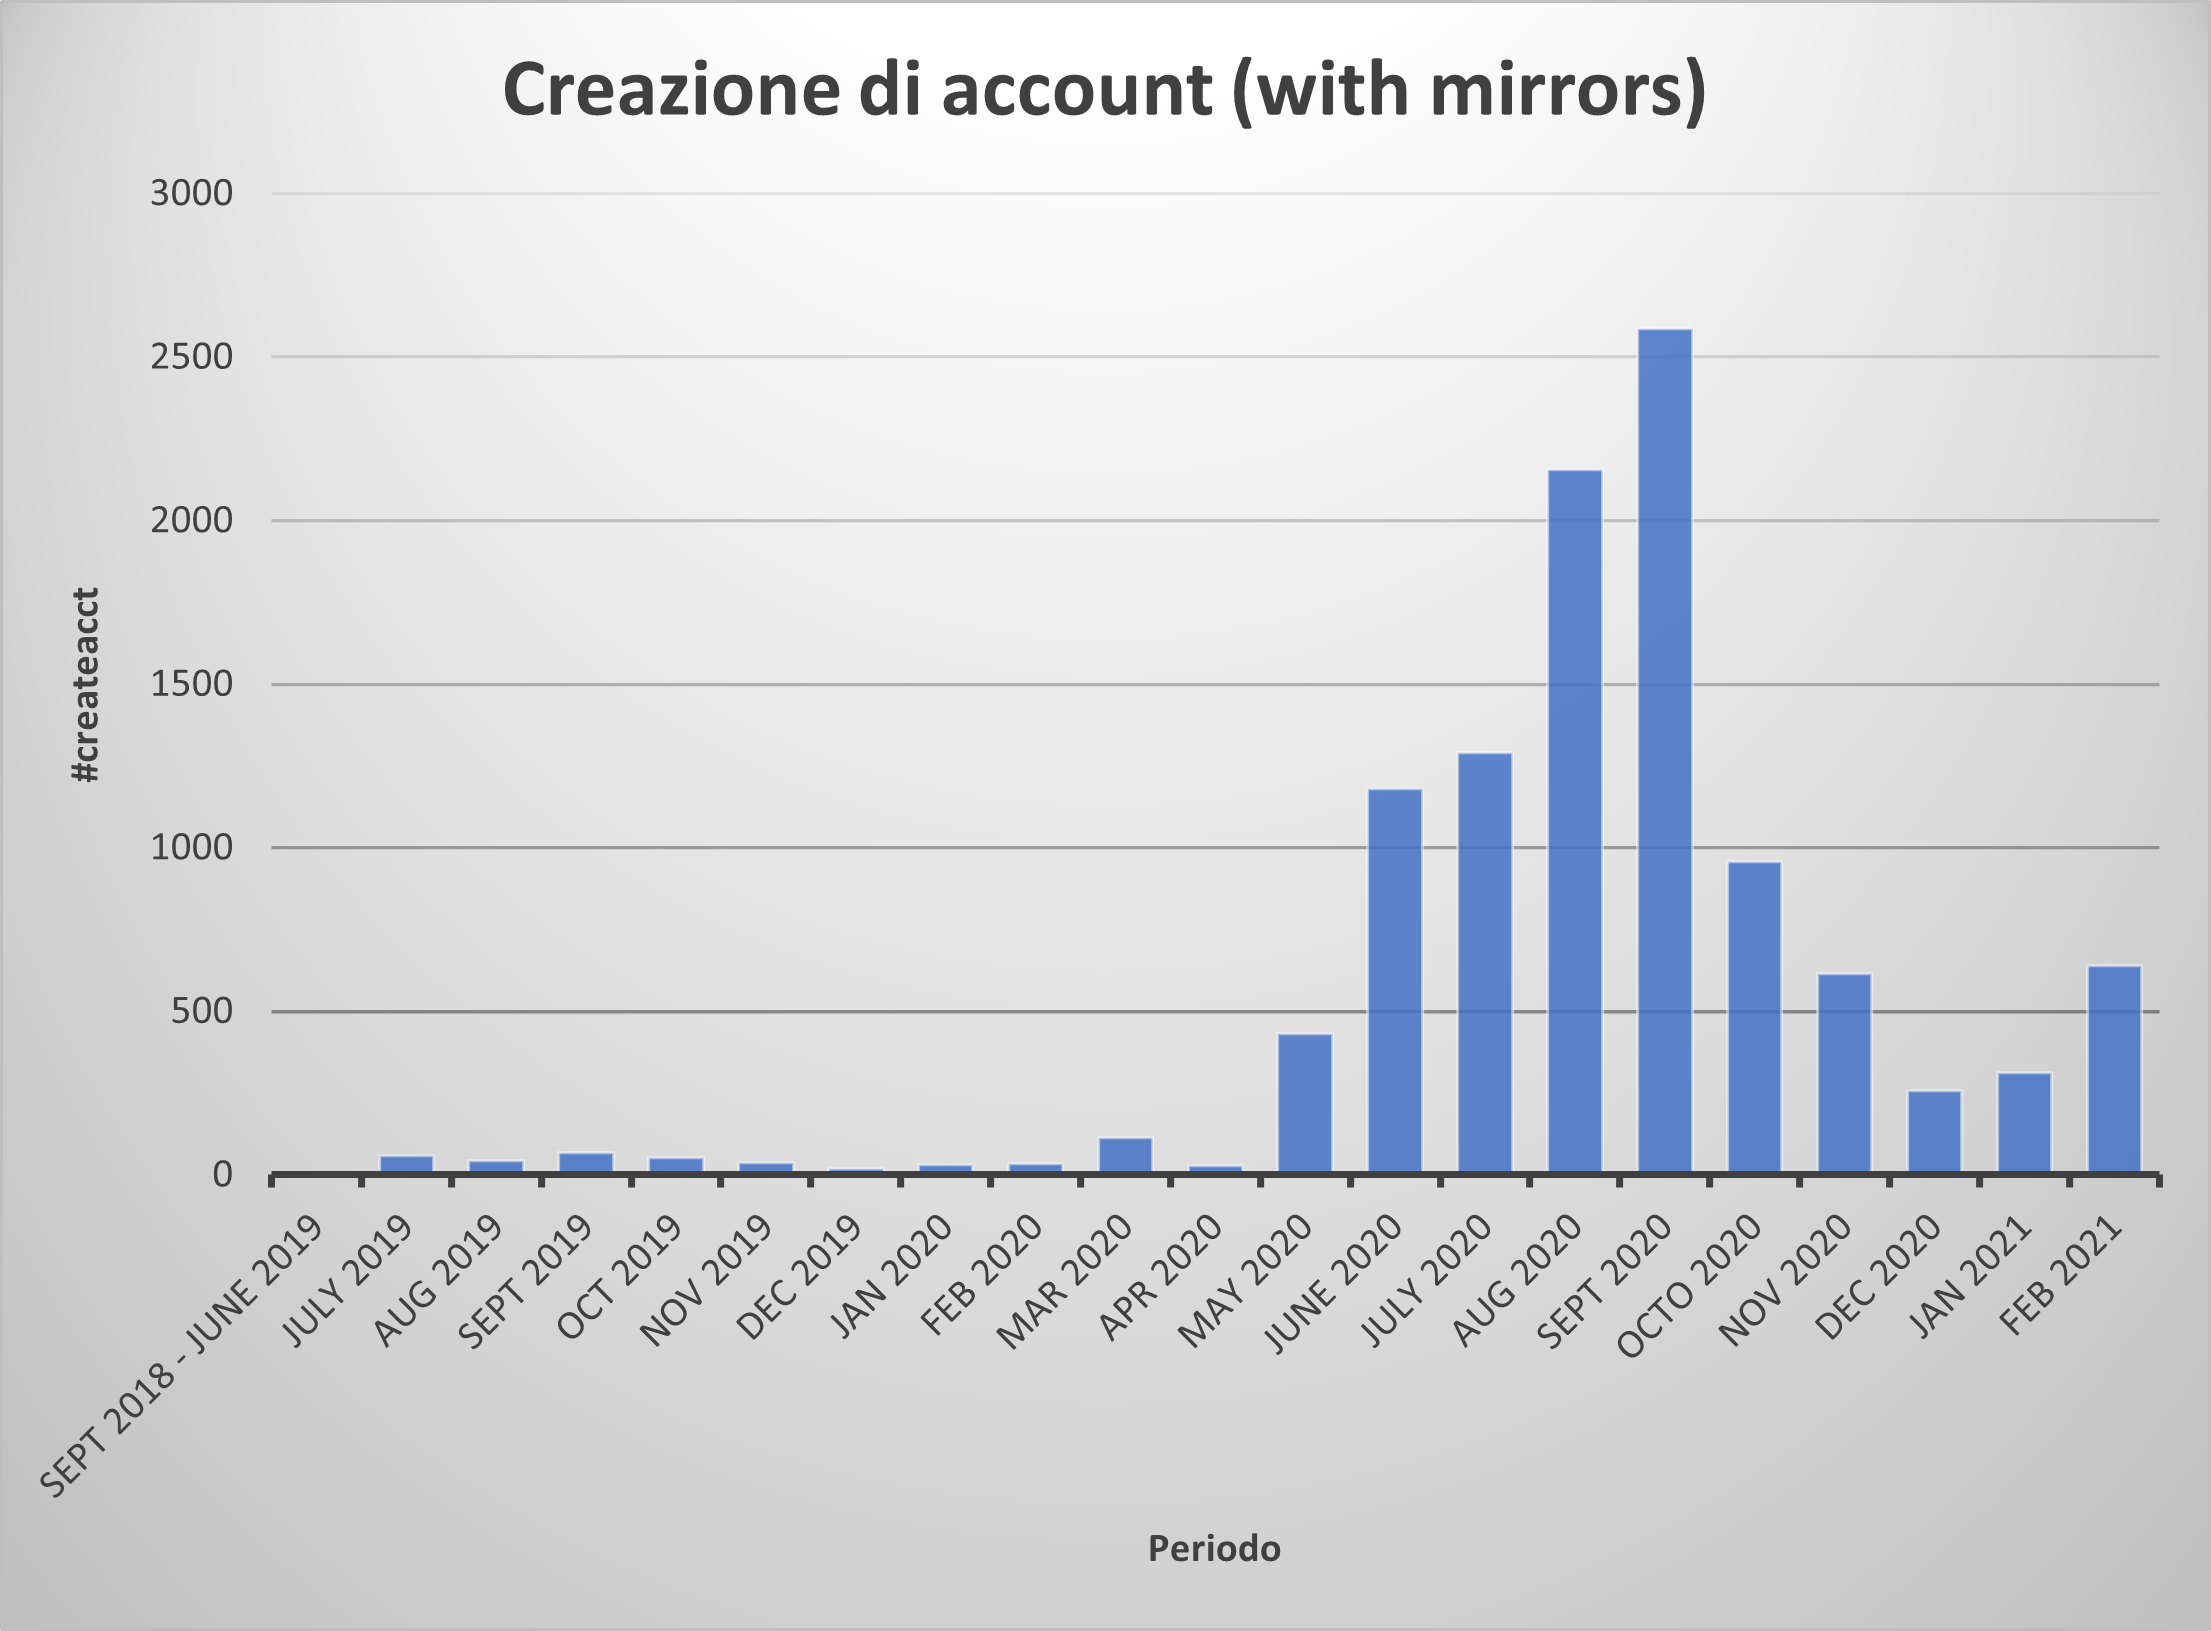
\includegraphics[width=.7\textwidth]{graphs/createaccount.png}
    \caption{Distribuzione mensile delle \textbf{createacct} includendo account Mirror}
    \label{fig:createacctMensile_conmirr}
\end{figure}

\begin{figure}[t]
    \centering
    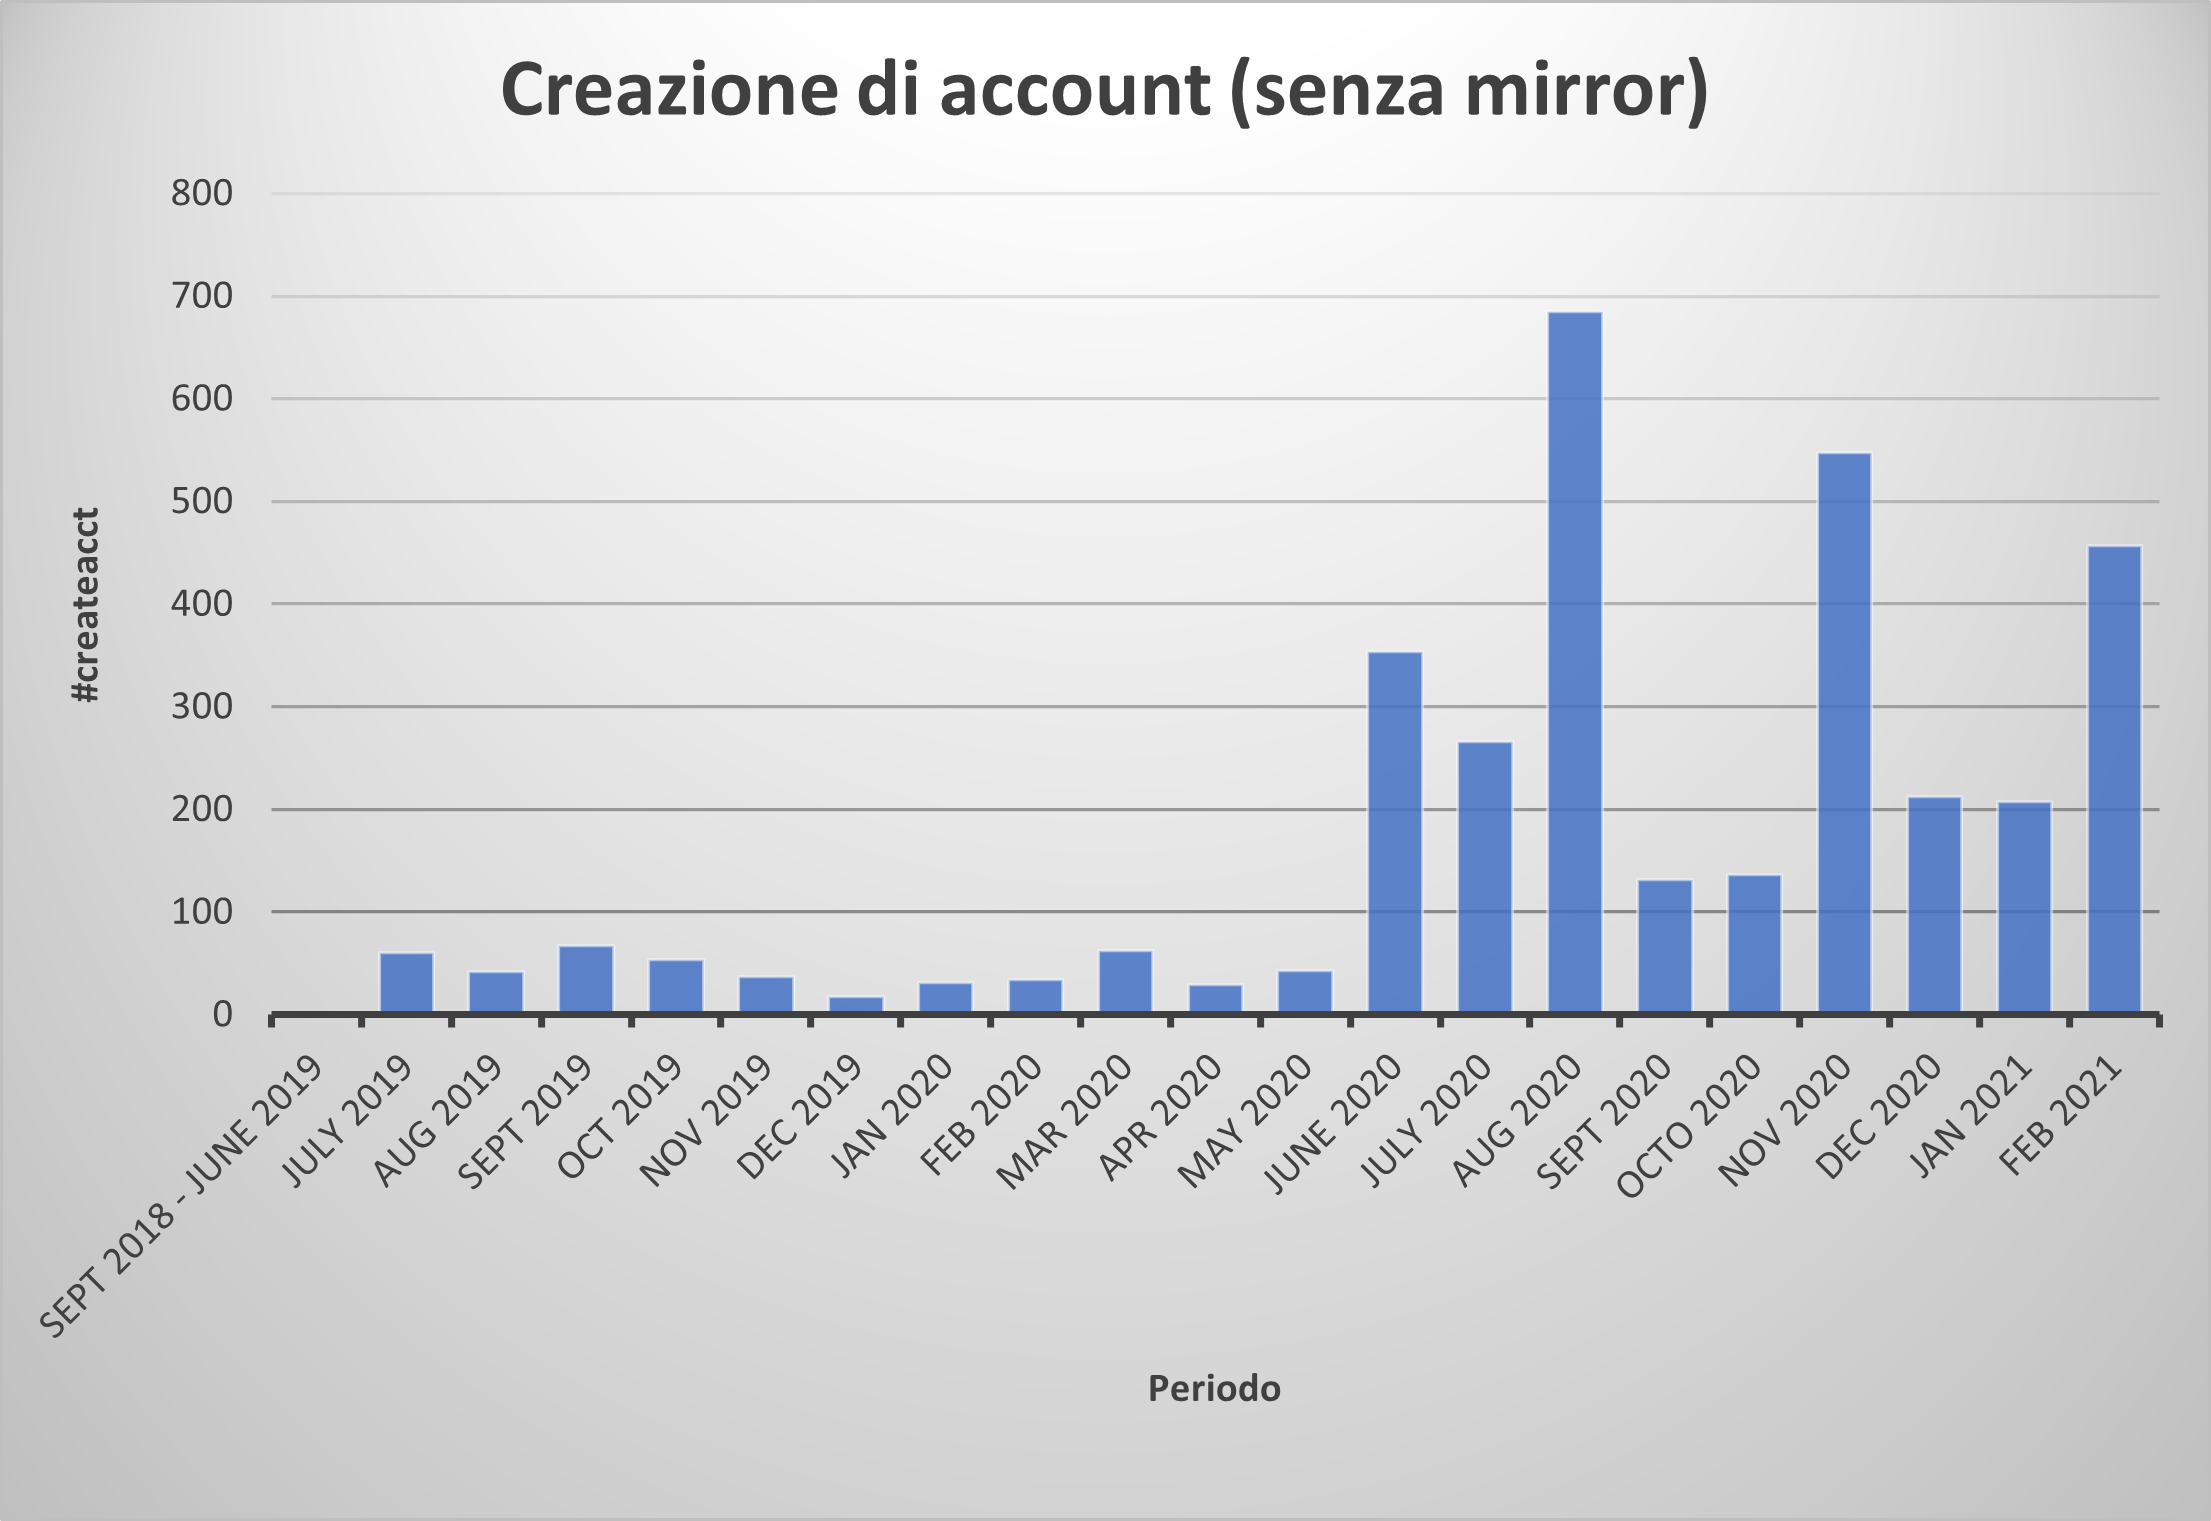
\includegraphics[width=.7\textwidth]{graphs/createaccount_nomirr.png}
    \caption{Distribuzione mensile delle \textbf{createacct} escludendo account Mirror}
    \label{fig:createacctMensile_nomirr}
\end{figure}

Non essendo a conoscenza dei criteri secondo cui vengono creati account Twitter Mirror su Yup è difficile avanzare ipotesi riguardo al grafico in Figura \ref{fig:createacctMensile_conmirr}. Possiamo tuttavia notare come fino ad Aprile 2020 la creazione di account, Mirror e non, fosse molto esigua se la paragoniamo a quella nei mesi successivi. Tra i mesi di Maggio 2020 e Novembre 2020 notiamo almeno 500 createacct al mese, con un picco di oltre 2.500 nuove creazioni nel solo mese di Settembre 2020, indice di come la piattaforma avesse iniziato a prendere piede grazie alle campagne pubblicitarie e all'inizio della fase beta aperta a tutti.
%Anche in questo caso il picco osservabile in entrambi i casi nei mesi di Agosto-Settembre potrebbe essere invece correlato al lancio della piattaforma in Ottobre.

Paragonando le Figure \ref{fig:createacctMensile_conmirr} e \ref{fig:createacctMensile_nomirr} notiamo che una larga porzione dei nuovi account sulla piattaforma proprio nel periodo Giugno 2020 - Novembre 2020 è formata da account Mirror.
Attribuiamo questo fenomeno a strategie utilizzate dai creatori di Yup per invogliare nuovi utenti ad unirsi alla piattaforma, mostrando quanto è possibile guadagnare.

\subsection{Utenti attivi-passivi}
Infine abbiamo analizzato, su base mensile, l'attività degli utenti facendo una classificazione in utenti attivi o passivi. Con \textbf{utenti attivi} indichiamo coloro che hanno effettuato un'azione di voto, follow, commento o modifica della biografia del proprio account in un dato periodo temporale, mentre con \textbf{utenti passivi} quelli che hanno effettuato solamente un'operazione di login. Un appunto che deve essere fatto è che quest'ultima classificazione è solo parziale poiché alcuni utenti potrebbero aver effettuato il login sulla piattaforma e successivamente non aver fatto nulla, quindi essere utenti passivi, ma tale azione non viene registrata sul protocollo perché il login è automatizzato con le credenziali salvate nella cache del browser. Mostriamo in Figura \ref{fig:attivi_conmirr} gli utenti attivi e passivi includendo gli account Mirror, e in Figura \ref{fig:attivi_nomirr} gli utenti attivi e passivi escludendo gli account Mirror.

\begin{figure}[t]
    \centering
    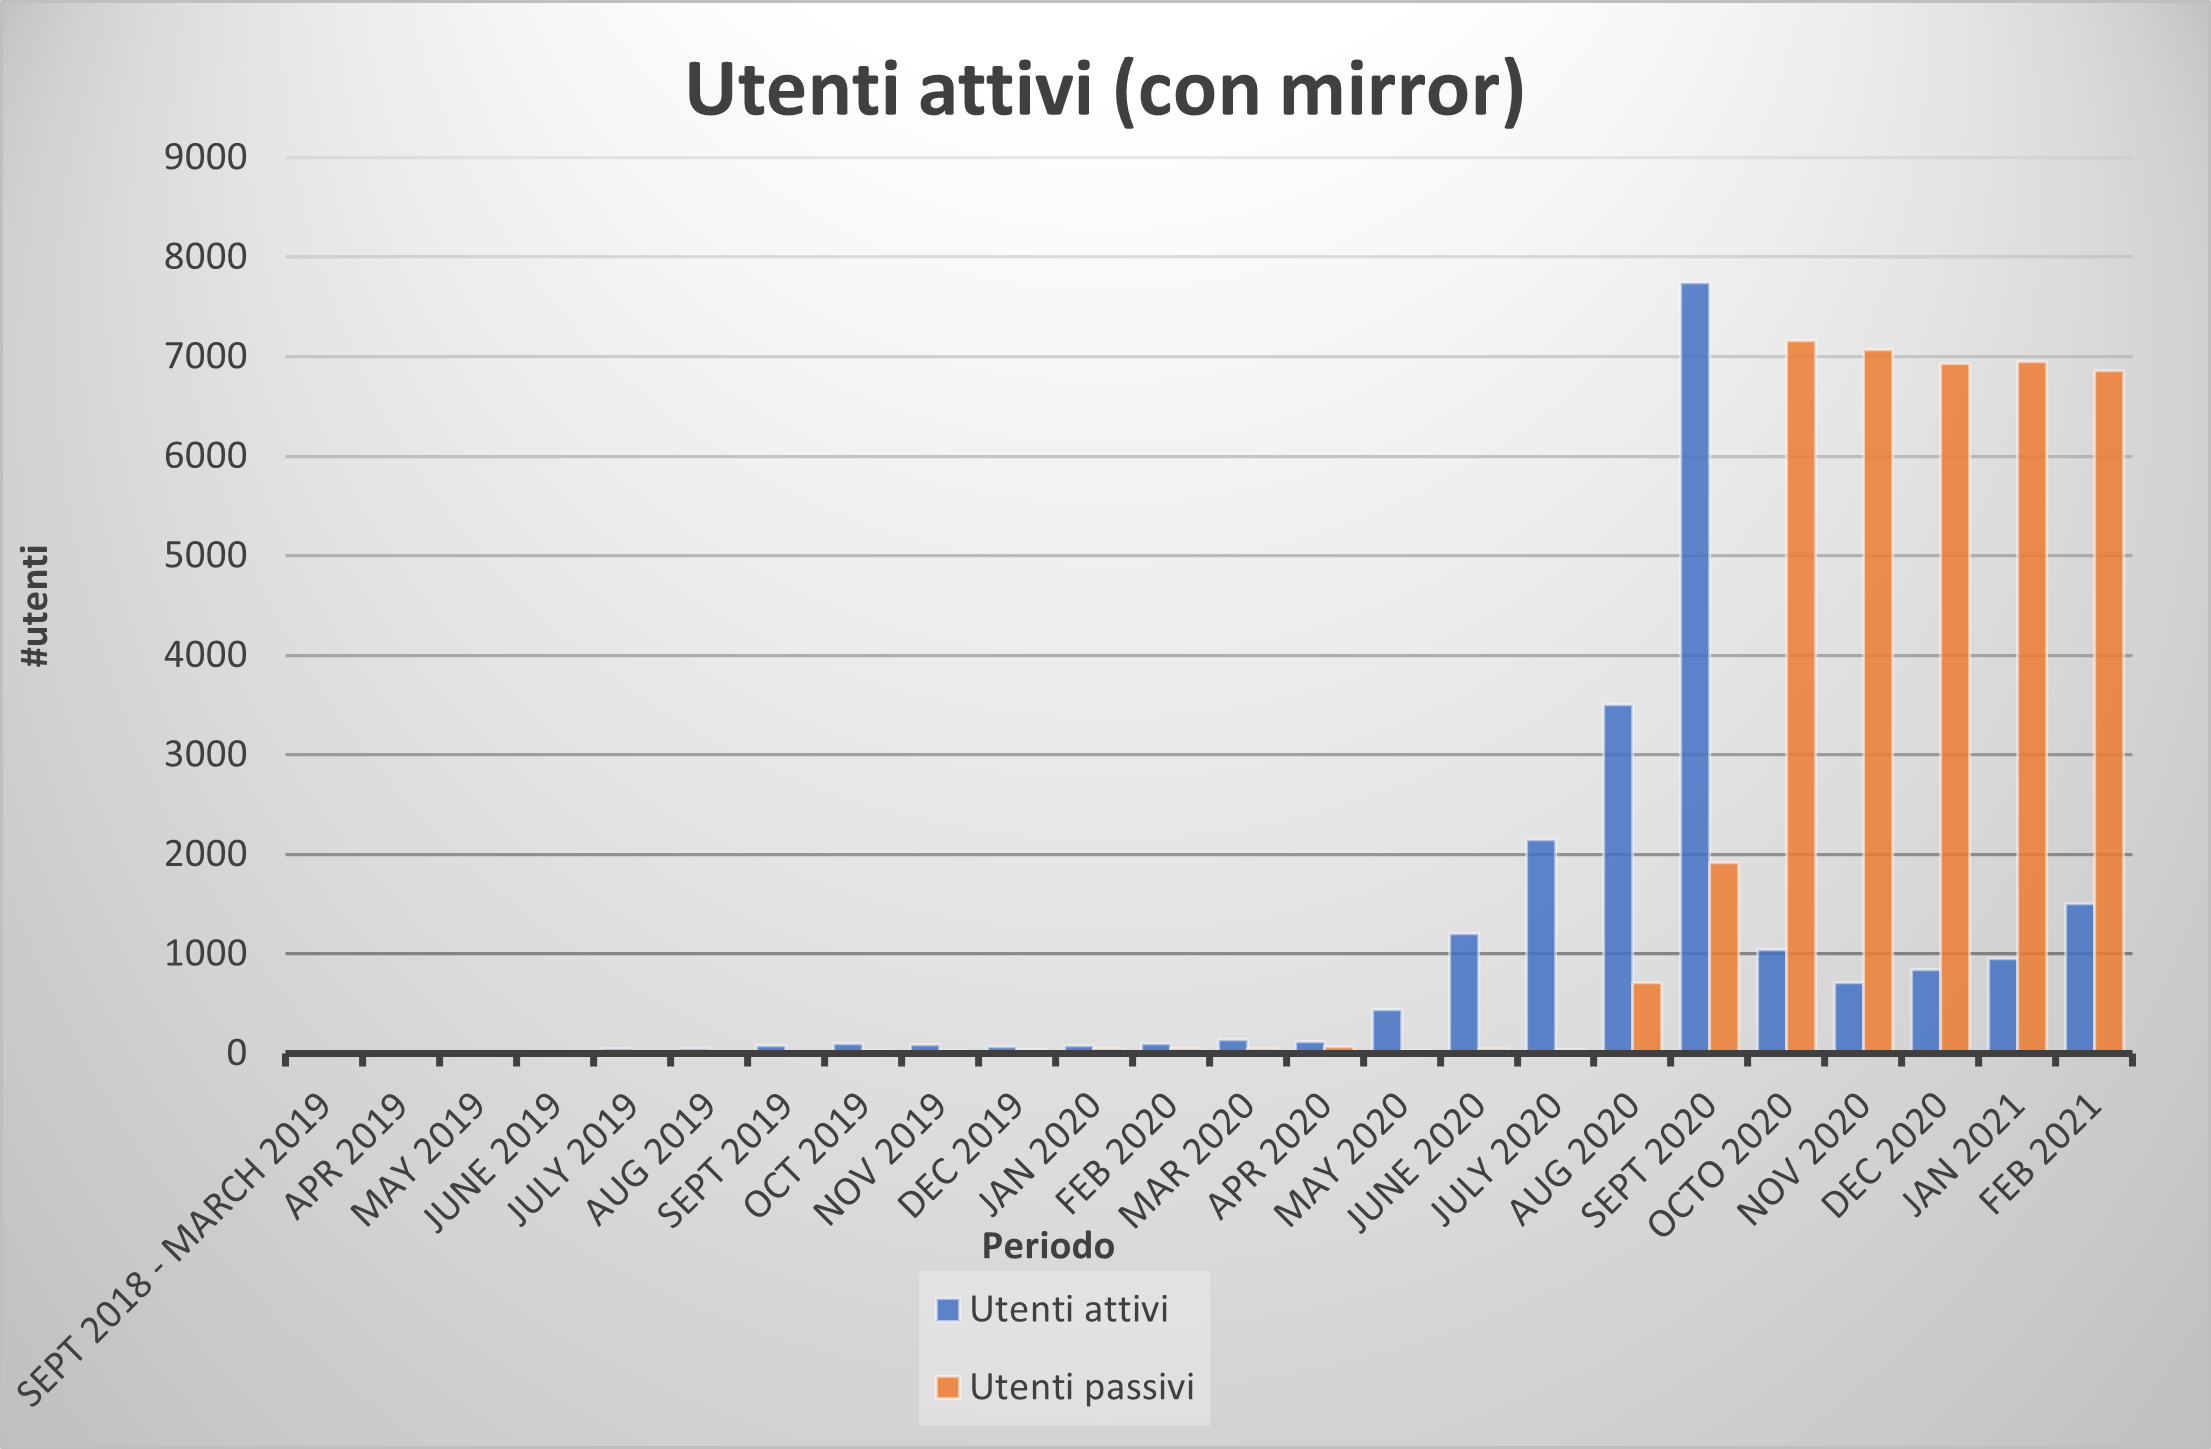
\includegraphics[width=0.7\textwidth]{graphs/utentiattivi.png}
    \caption{Utenti attivi-passivi su base mensile includendo account Mirror}
    \label{fig:attivi_conmirr}
\end{figure}

\begin{figure}[t]
    \centering
    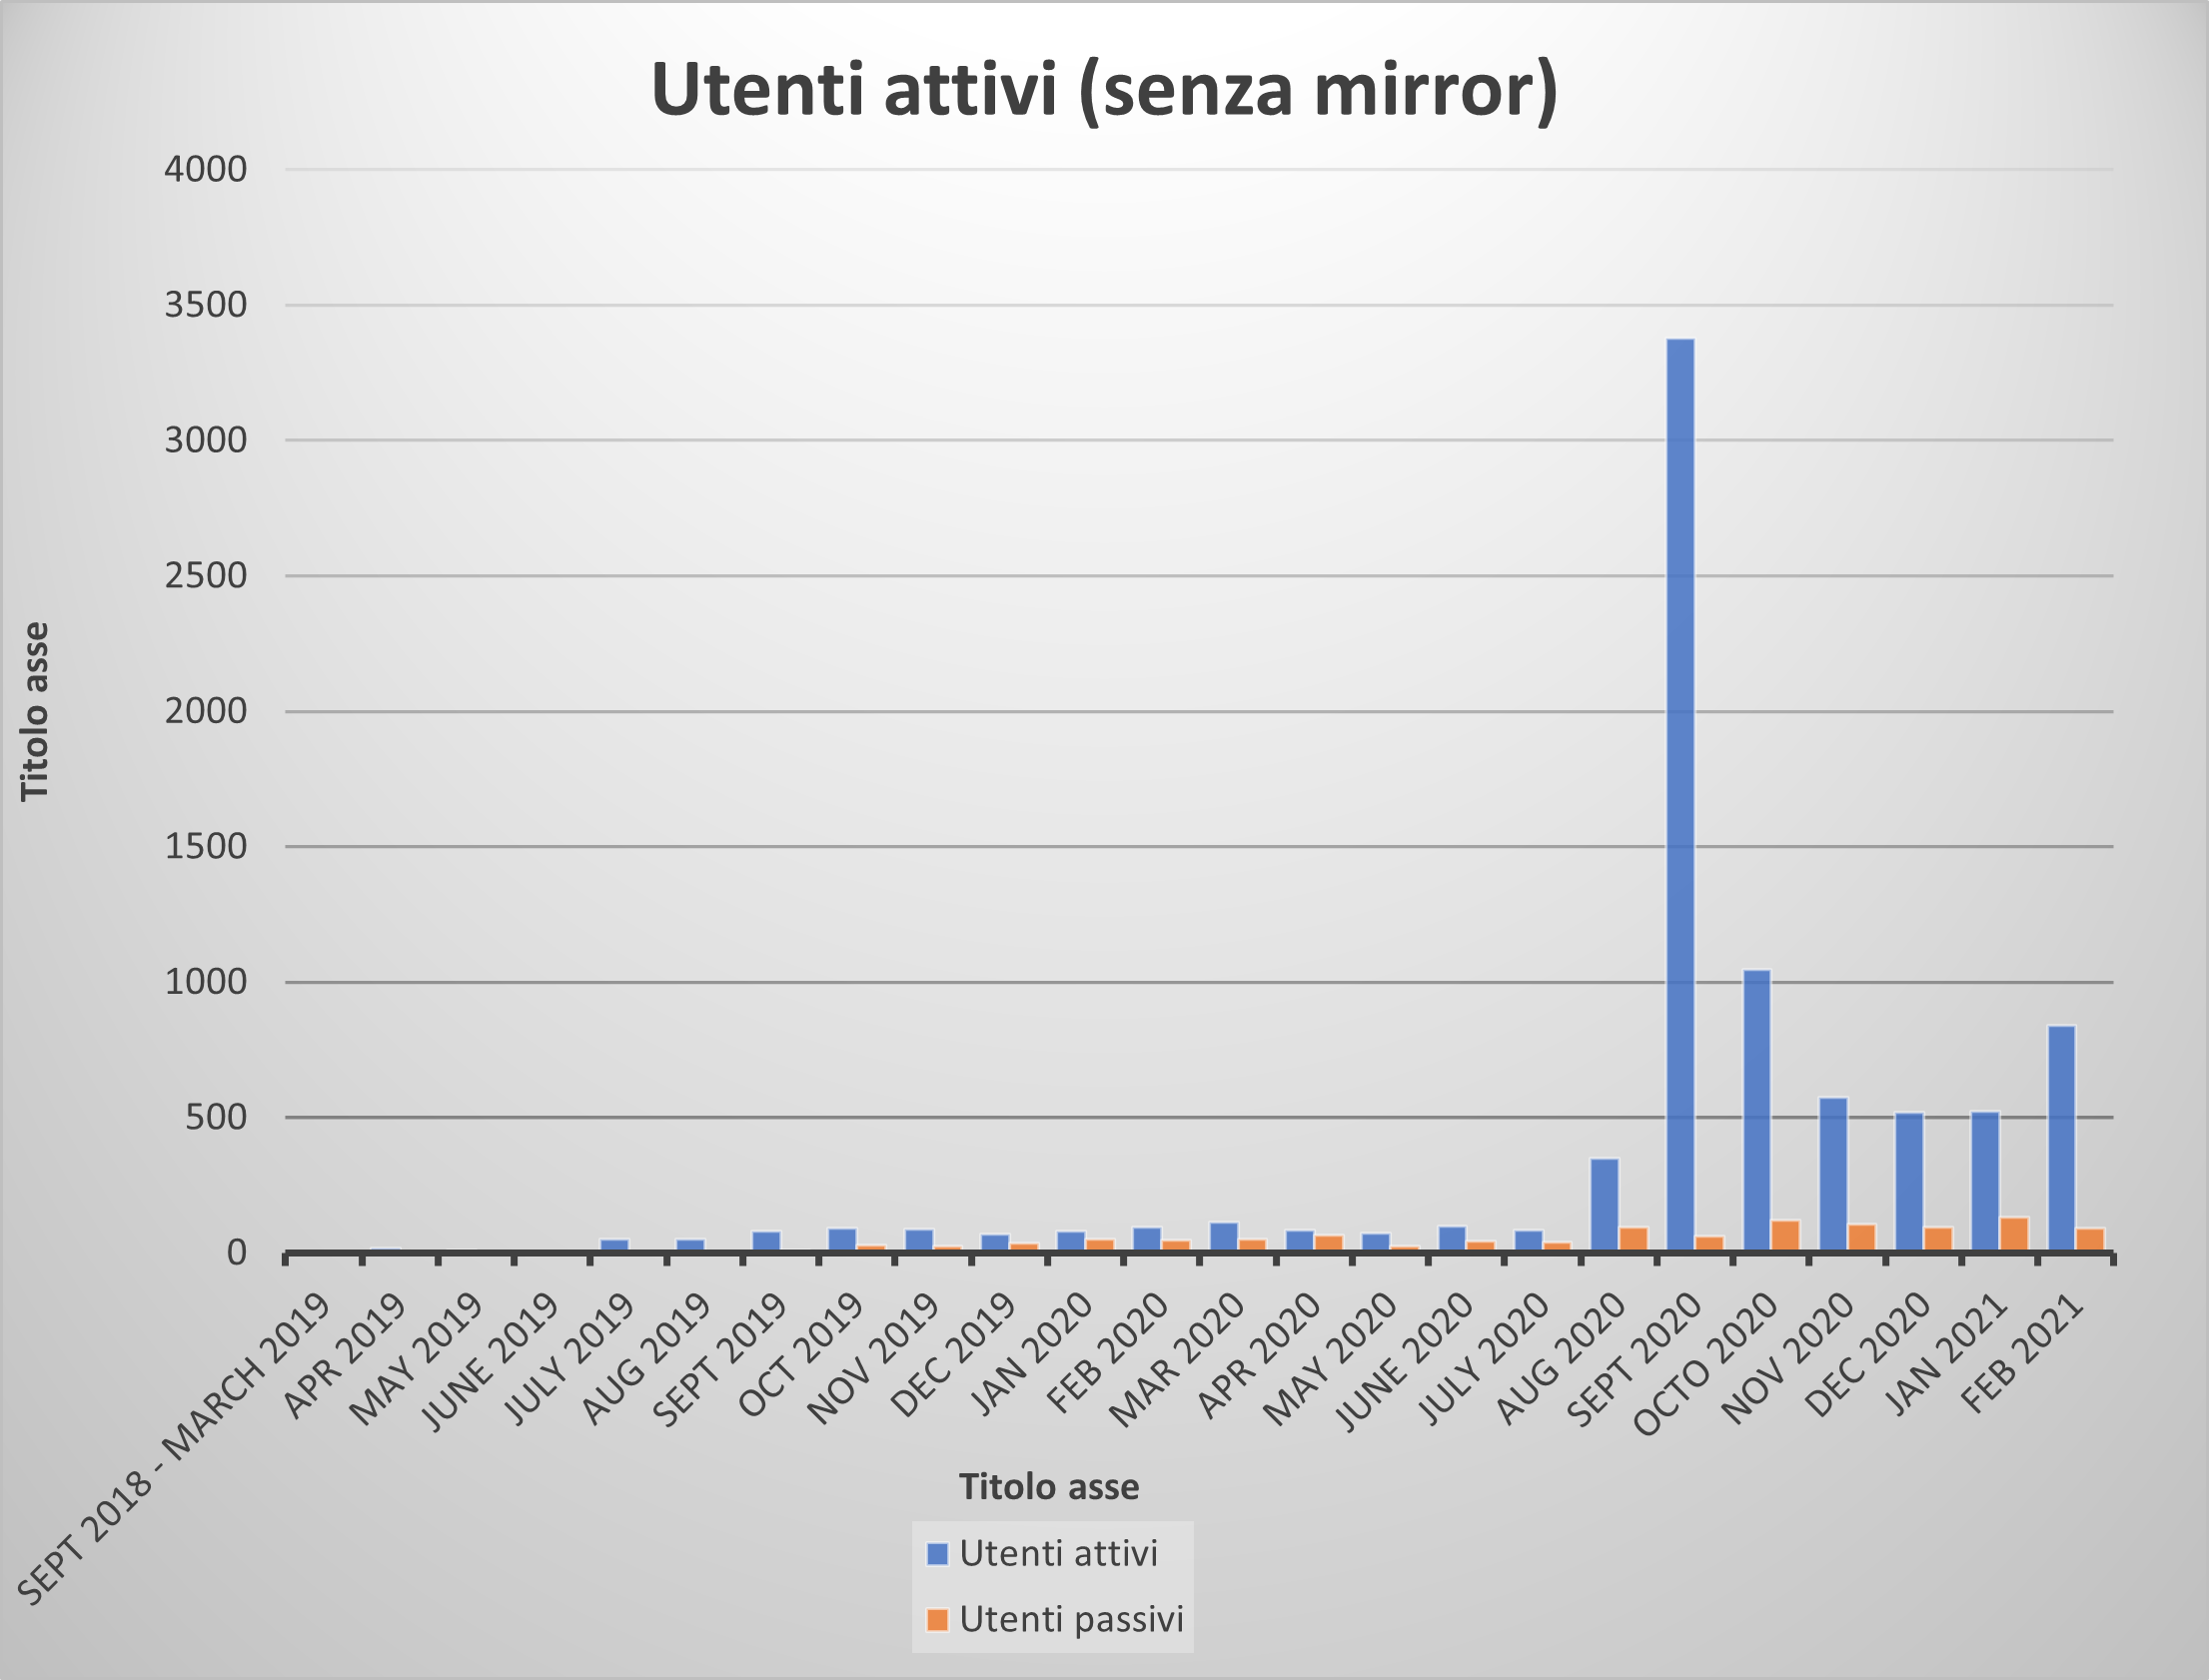
\includegraphics[width=0.7\textwidth]{graphs/utentiattivi_nomirr.png}
    \caption{Utenti attivi-passivi su base mensile escludendo account Mirror}
    \label{fig:attivi_nomirr}
\end{figure}

E' possibile notare come l'inclusione o l'esclusione degli account Mirror abbia un forte impatto sul conteggio degli account passivi. Confrontando le Figure constatiamo che, per la maggior parte degli account Mirror, non ci sia più un mirroring delle azioni che effettuano su Twitter, ma soltanto una continua ripetizione di azioni di login. A testimoniare questa supposizione vi è il fatto che, nel momento in cui consideriamo tali account, abbiamo un forte incremento degli account passivi in ogni mese. Inoltre, confrontando le Figure \ref{fig:attivi_conmirr} e \ref{fig:createacctMensile_conmirr}, possiamo notare come l'incremento di utenti attivi e passivi coincida proprio con i mesi nei quali abbiamo notato numerose inscrizioni di account Mirror, ovvero da Giugno 2020 a Settembre 2020.
D'altro canto, se consideriamo solo gli utenti non-Mirror, dopo il boom di iscrizioni rilevato nel mese di Settembre (vedi Figura \ref{fig:createacctMensile_nomirr}), il numero di utenti attivi rimane tra 500 e 1.000, mentre il numero di utenti inattivi rimane molto basso (Figura \ref{fig:attivi_nomirr}).

\section{Azioni di voto}
Dopo aver analizzato la natura dei vari account, insieme ad alcune caratteristiche chiave, come la creazione, volgiamo ora la nostra attenzione all'aspetto chiave della piattaforma Yup, ovvero i voti.
Come abbiamo visto nel Capitolo \ref{platform_chapter}, valutare i contenuti disponibili nel web è il motivo per cui Yup è stato proposto, e coincide inoltre con la maniera più importante per poter accumulare criptomoneta sulla piattaforma.
Questo impone di studiare in maniera dettagliata questa componente, e in particolare noi ci siamo concentrati sulle informazioni che i voti ci possono dare riguardo l'attività degli utenti e riguardo le piattaforme più valutate.

L'analisi dell'attività di votazione tiene conto delle sole azioni (createvote|v2|v3|v4 e postvote|v2|v3|v4), in quanto relative all'espressione di un voto.
Ricordiamo che le azioni createvote corrispondono a dei voti per contenuti precedentemente già votati almeno una volta, mentre le azioni postvote corrispondono a voti per contenuti precedentemente mai votati, come spiegato nel Capitolo \ref{platform_chapter}.
Anche in questo caso effettuiamo una distinzione tra quelle relative ad account Mirror e quelle relative ad account non-Mirror, mostrate in Tabella \ref{tab:votingactionsDistribution}.

\begin{table}
\centering
\begin{tabular}{ |c|c|c|c| }
 \hline
  & Totale & Mirror & non-Mirror \\
 \hline
 AZIONI DI VOTO & 497.526 & 180.371 & 317.155 \\
 \hline
 CREATEVOTE & 316.246 & 114.947 & 201.299 \\
 \hline
 POSTVOTE & 181.280 & 65.424 & 115.856 \\
 \hline
\end{tabular}
\caption{Distribuzione azioni di voto per account Mirror e non}
\label{tab:votingactionsDistribution}
\end{table}

La Tabella mostra che sotto il punto di vista della valutazione dei contenuti, gli account Mirror sono meno attivi rispetto agli account non-Mirror, nonostante il loro numero sia paragonabile, come mostrato in Tabella \ref{table:usersClassification}. Questo è principalmente dovuto al fatto che gli account Mirror sono account automatizzati e gestiti dagli sviluppatori di Yup al posto delle celebrità che questi account rappresentano e la loro attività deve rispecchiare l'account originale.
Notiamo inoltre che le azioni della famiglia createvote sono poco meno del doppio delle postvote.
Considerata la loro differente funzione, ci possiamo aspettare che le catene di voti formate da postvote e createvote siano corte e che in media per ogni postvote ci siano due createvote.


E' stato inoltre individuato un numero di votatori unici pari a \textbf{5.196}. Considerato come questo numero sia superiore a quello degli account non-Mirror creati tramite interazione con il protocollo (\textit{$3.475$}), ci porta alla conclusione che anche gli account che non sono stati originati da una createacct possono votare/utilizzare la piattaforma.


Di seguito mostriamo la distribuzione mensile delle azioni di voto includendo i Mirror, in Fgura \ref{fig:votingMensile_conmirr}, ed escludendo i Mirror in Figura \ref{fig:votingMensile_nomirr}.

\begin{figure}[t]
    \centering
    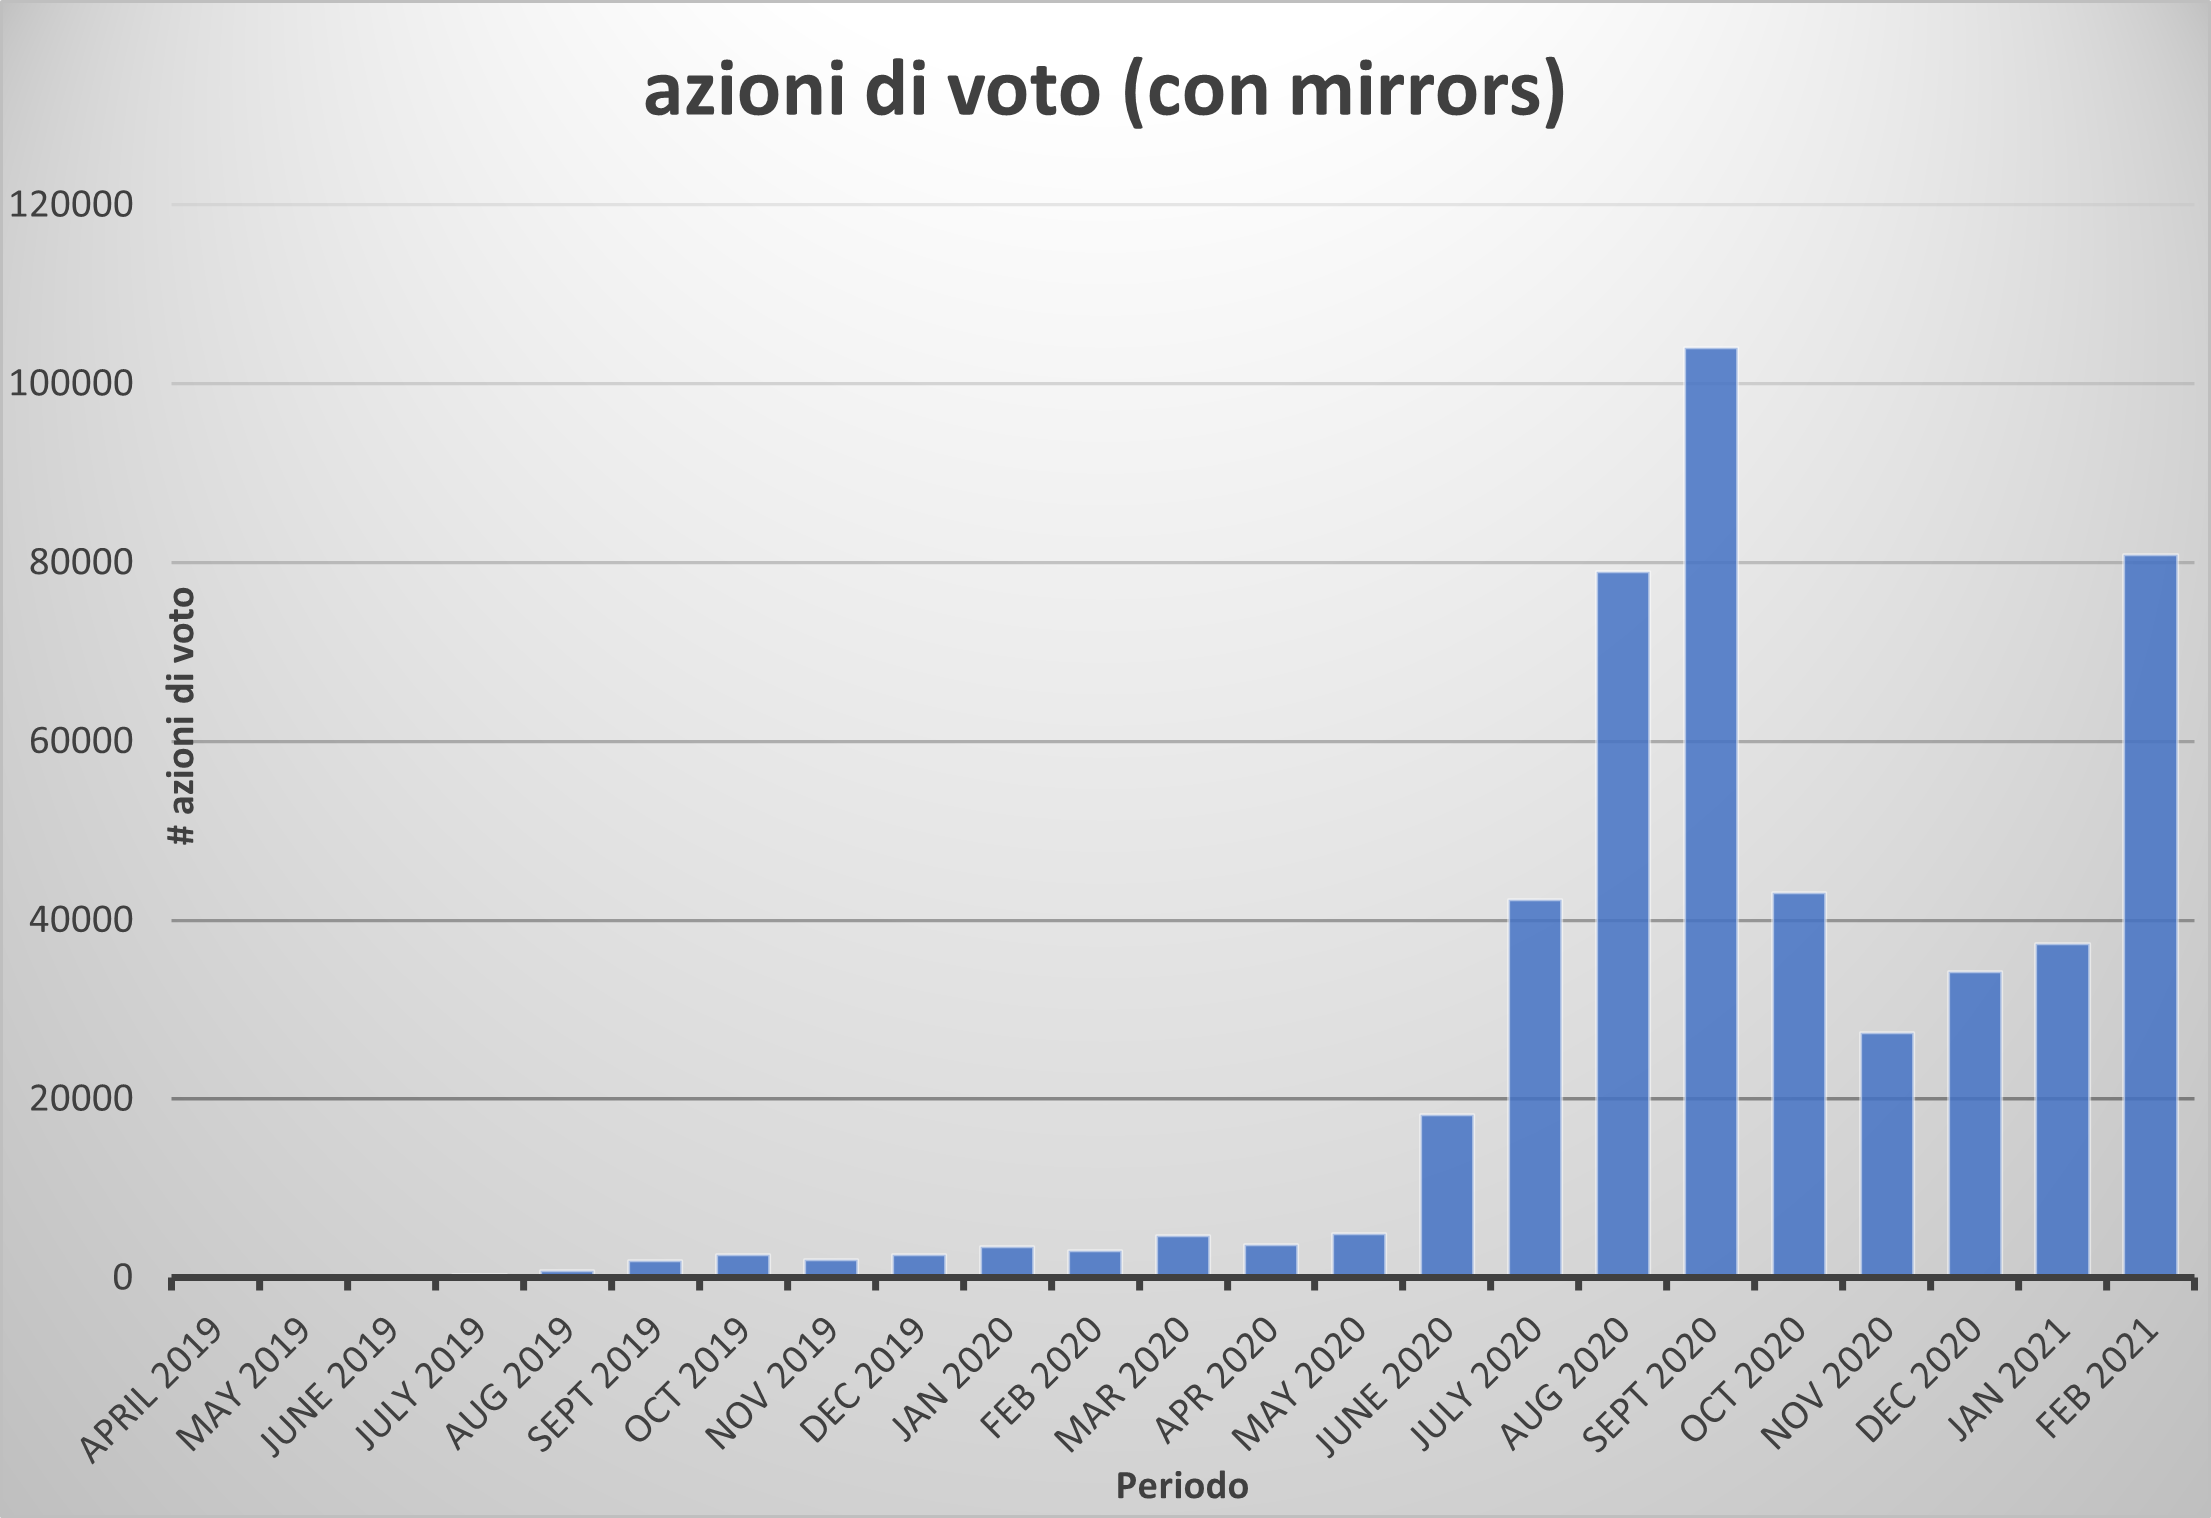
\includegraphics[width=.7\textwidth]{graphs/azioni_voto}
    \caption{Distribuzione mensile delle azioni di voto includendo account Mirror.}
    \label{fig:votingMensile_conmirr}
\end{figure}

\begin{figure}[t]
    \centering
    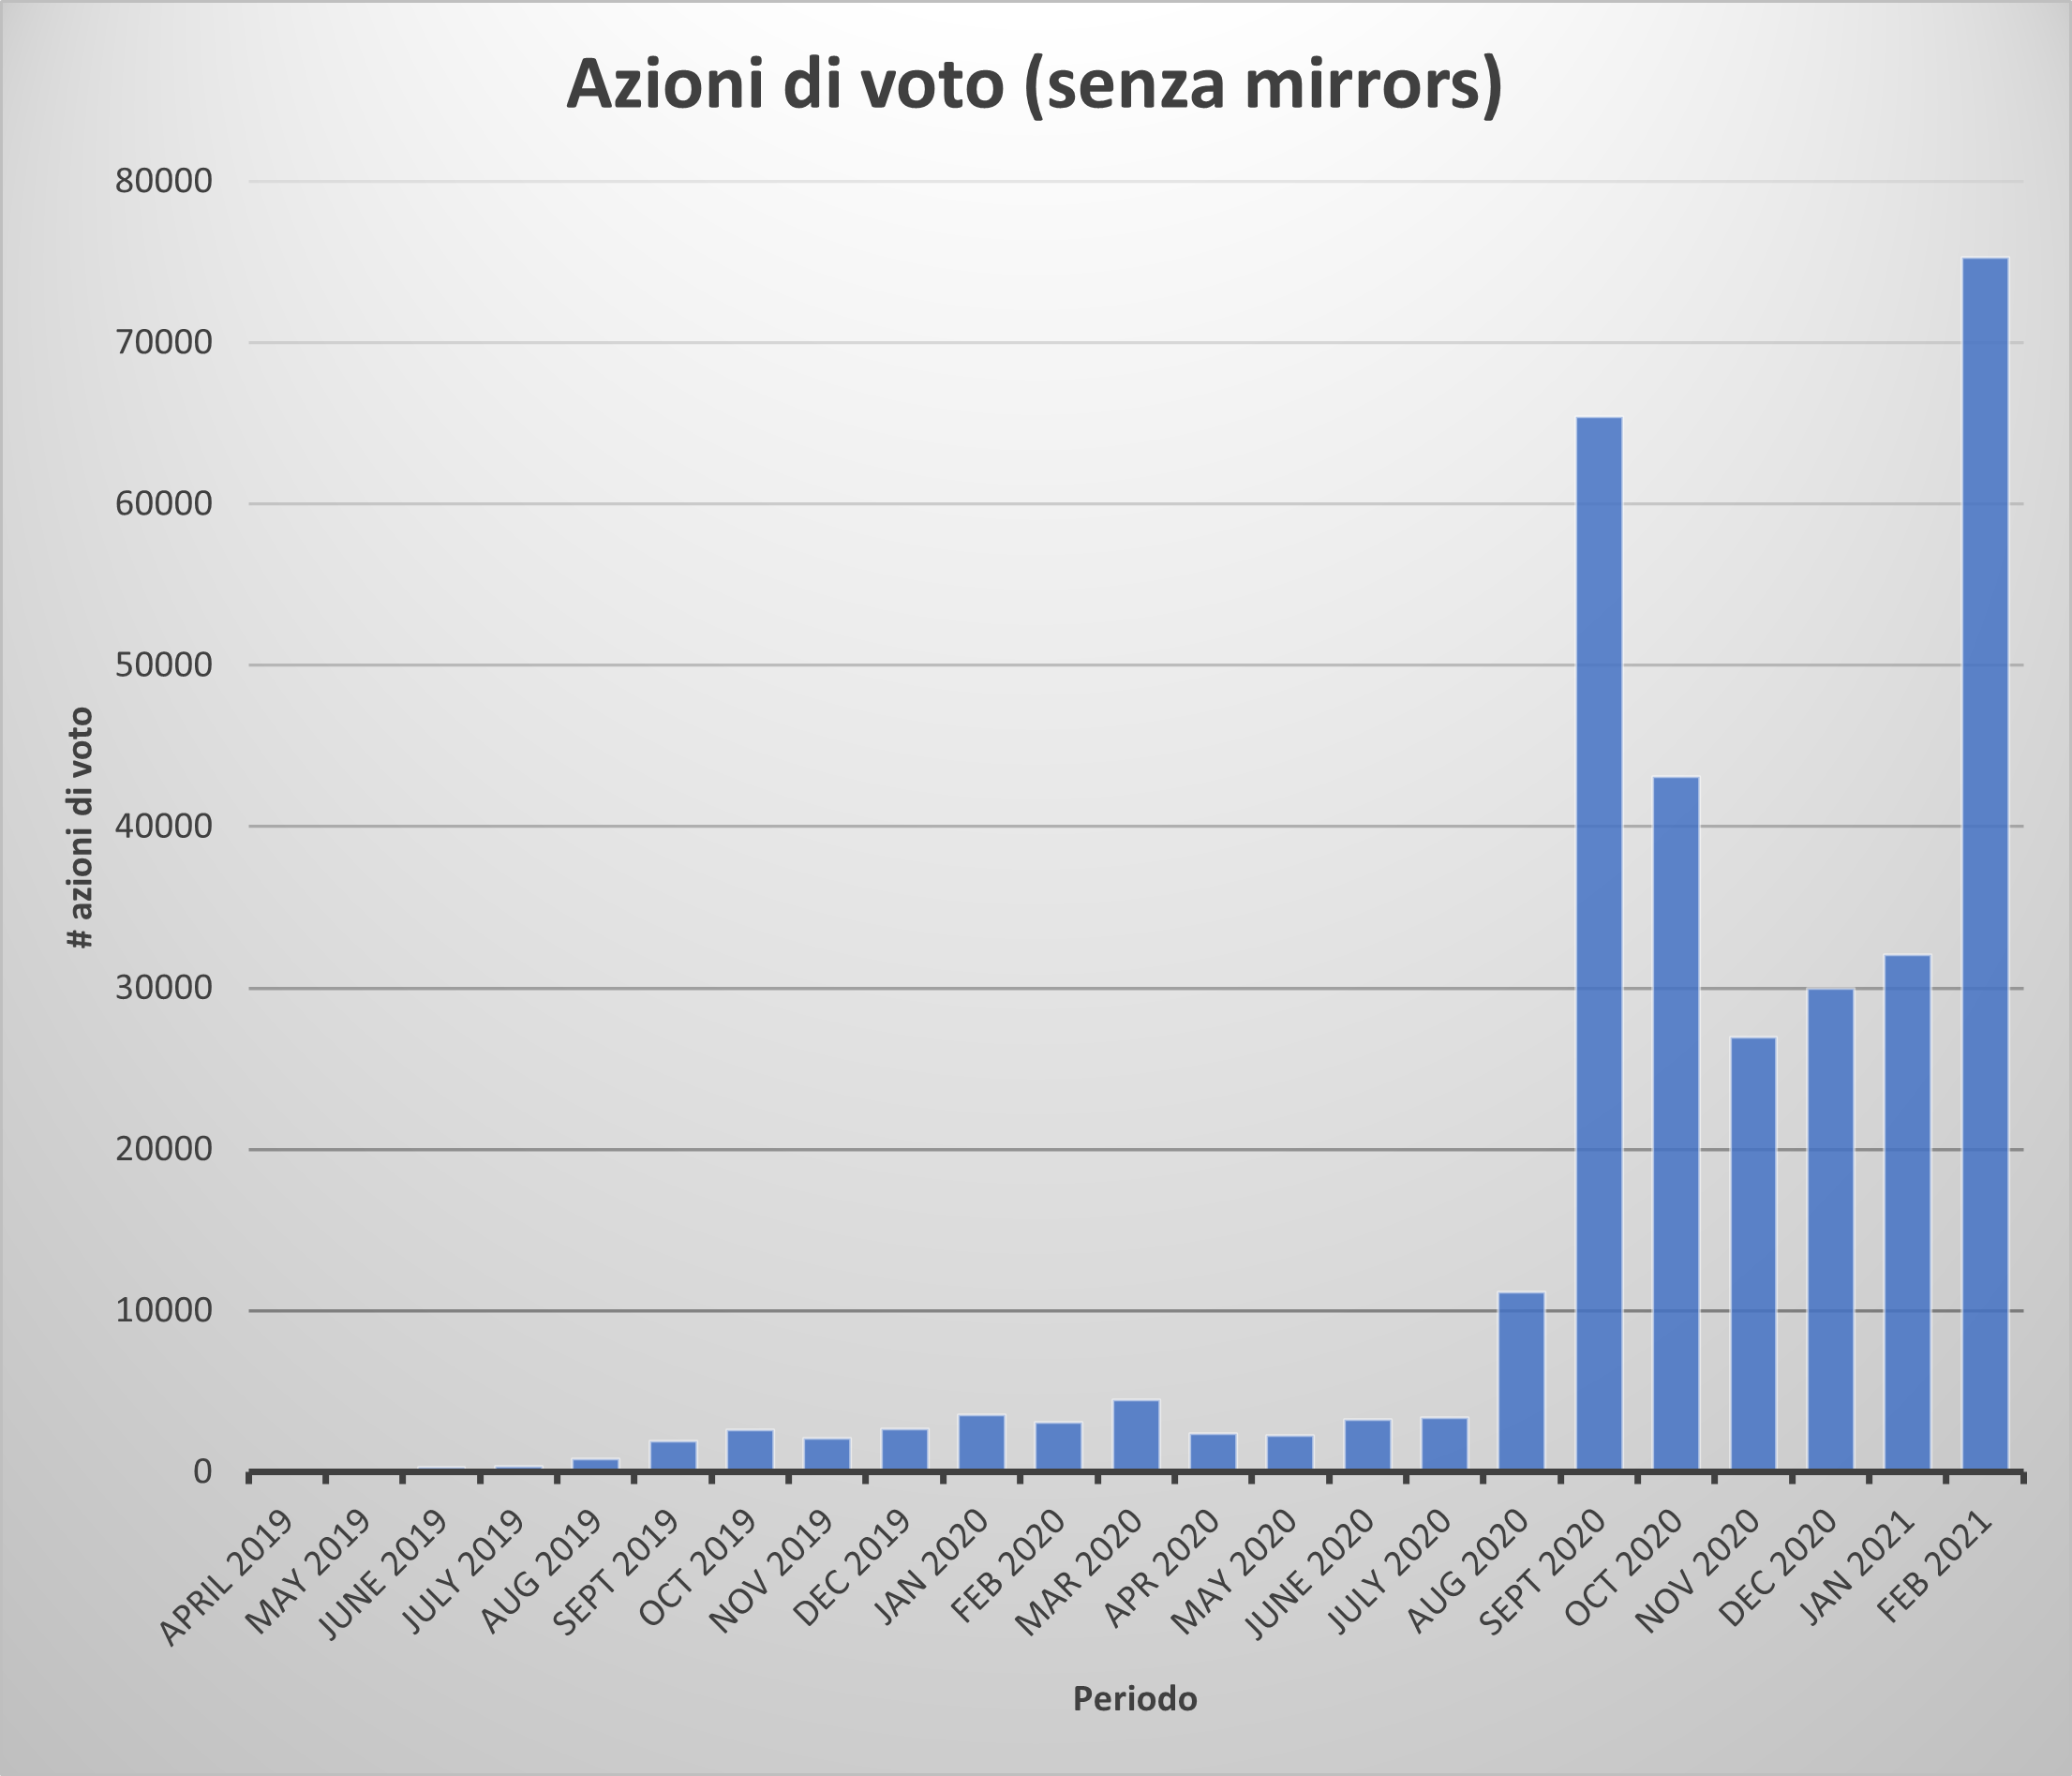
\includegraphics[width=.7\textwidth]{graphs/azioni_voto_nomirr}
    \caption{Distribuzione mensile delle azioni di voto escludendo account Mirror}
    \label{fig:votingMensile_nomirr}
\end{figure}

In questa analisi, come nelle precedenti, abbiamo un notevole incremento dell'attività nel periodo che precede il lancio della piattaforma. Notiamo infatti dei picchi notevoli nei mesi di Agosto e Settembre, che potremmo anche questa volta correlare al lancio di Yup, e successivamente nel mese di Febbraio, che testimonia una costante crescita dell'utilizzo del servizio da parte degli utenti.

Infine proponiamo una rappresentazione, sempre su base mensile, dei votatori unici individuati, ovvero utenti che hanno votato almeno un contenuto.
Mostriamo in Figura \ref{fig: uniquevoters_onlymirr} i votatori unici considerando solo account Mirror e in Figura \ref{fig: uniquevoters_nomirr} i votatori unici considerando solo account non-Mirror.

\begin{figure}[t]
    \centering
    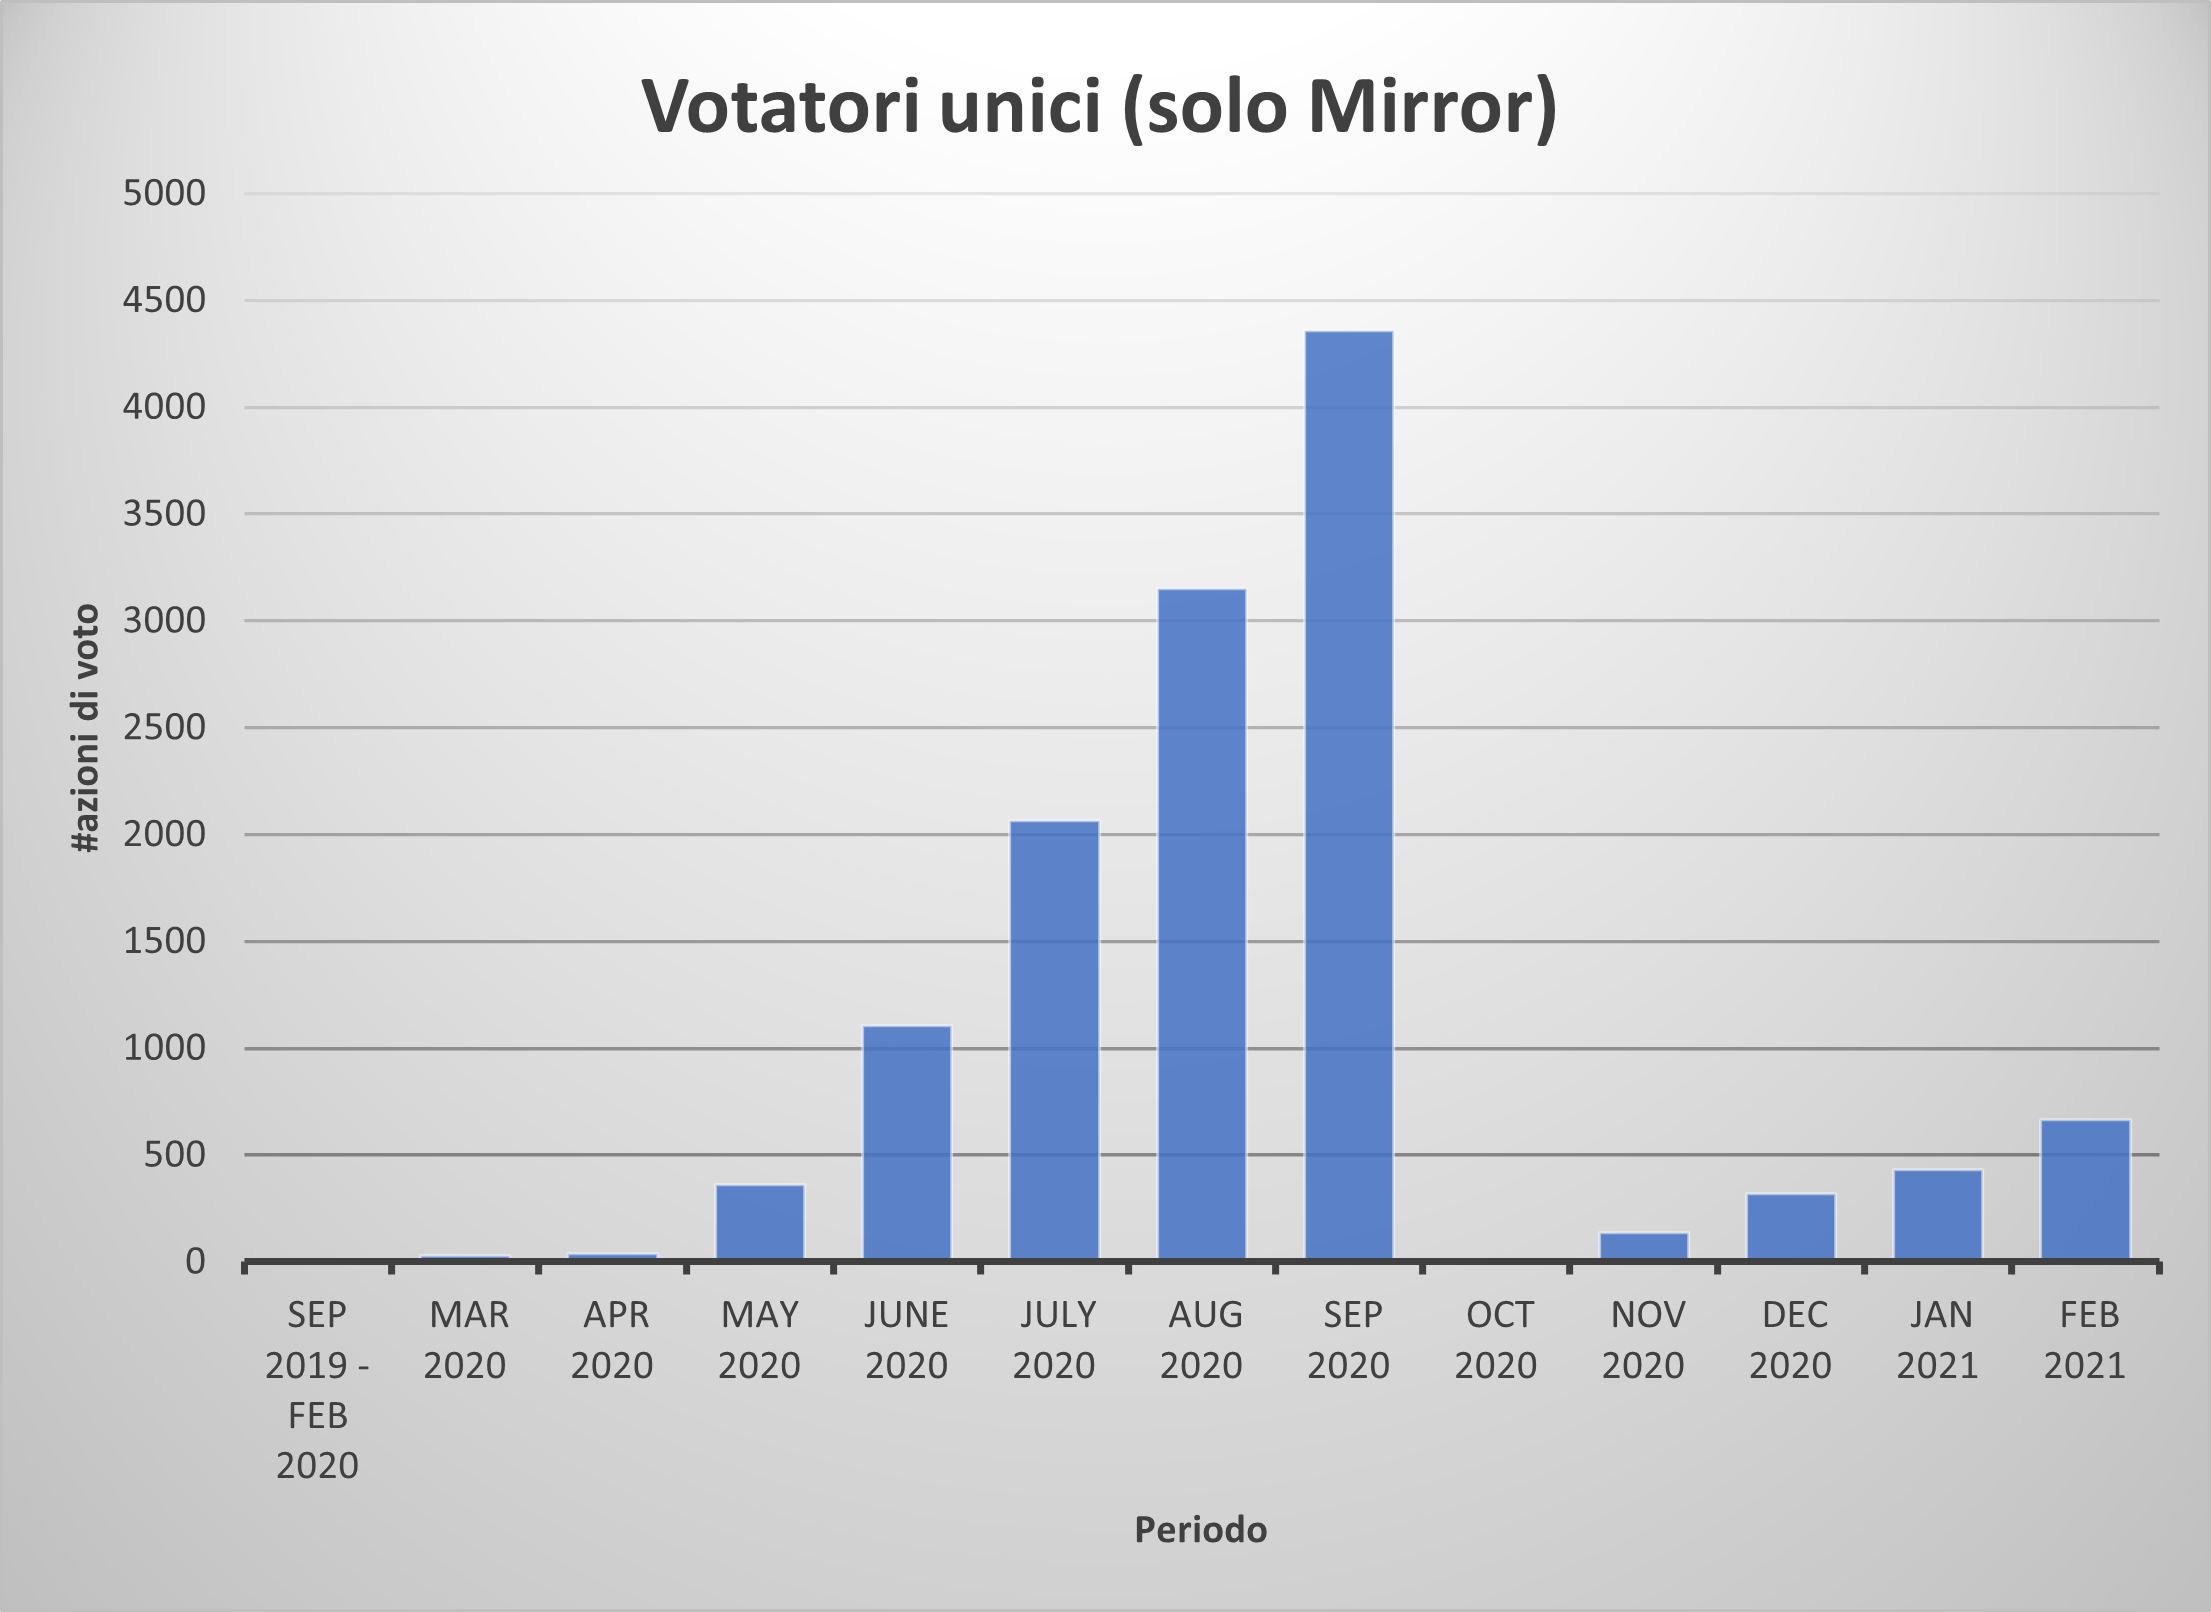
\includegraphics[width=.7\textwidth]{graphs/votatori_onlymirr.png}
    \caption{Rappresentazione mensile dei votatori unici, solo account Mirror}
    \label{fig: uniquevoters_onlymirr}
\end{figure}

\begin{figure}[t]
    \centering
    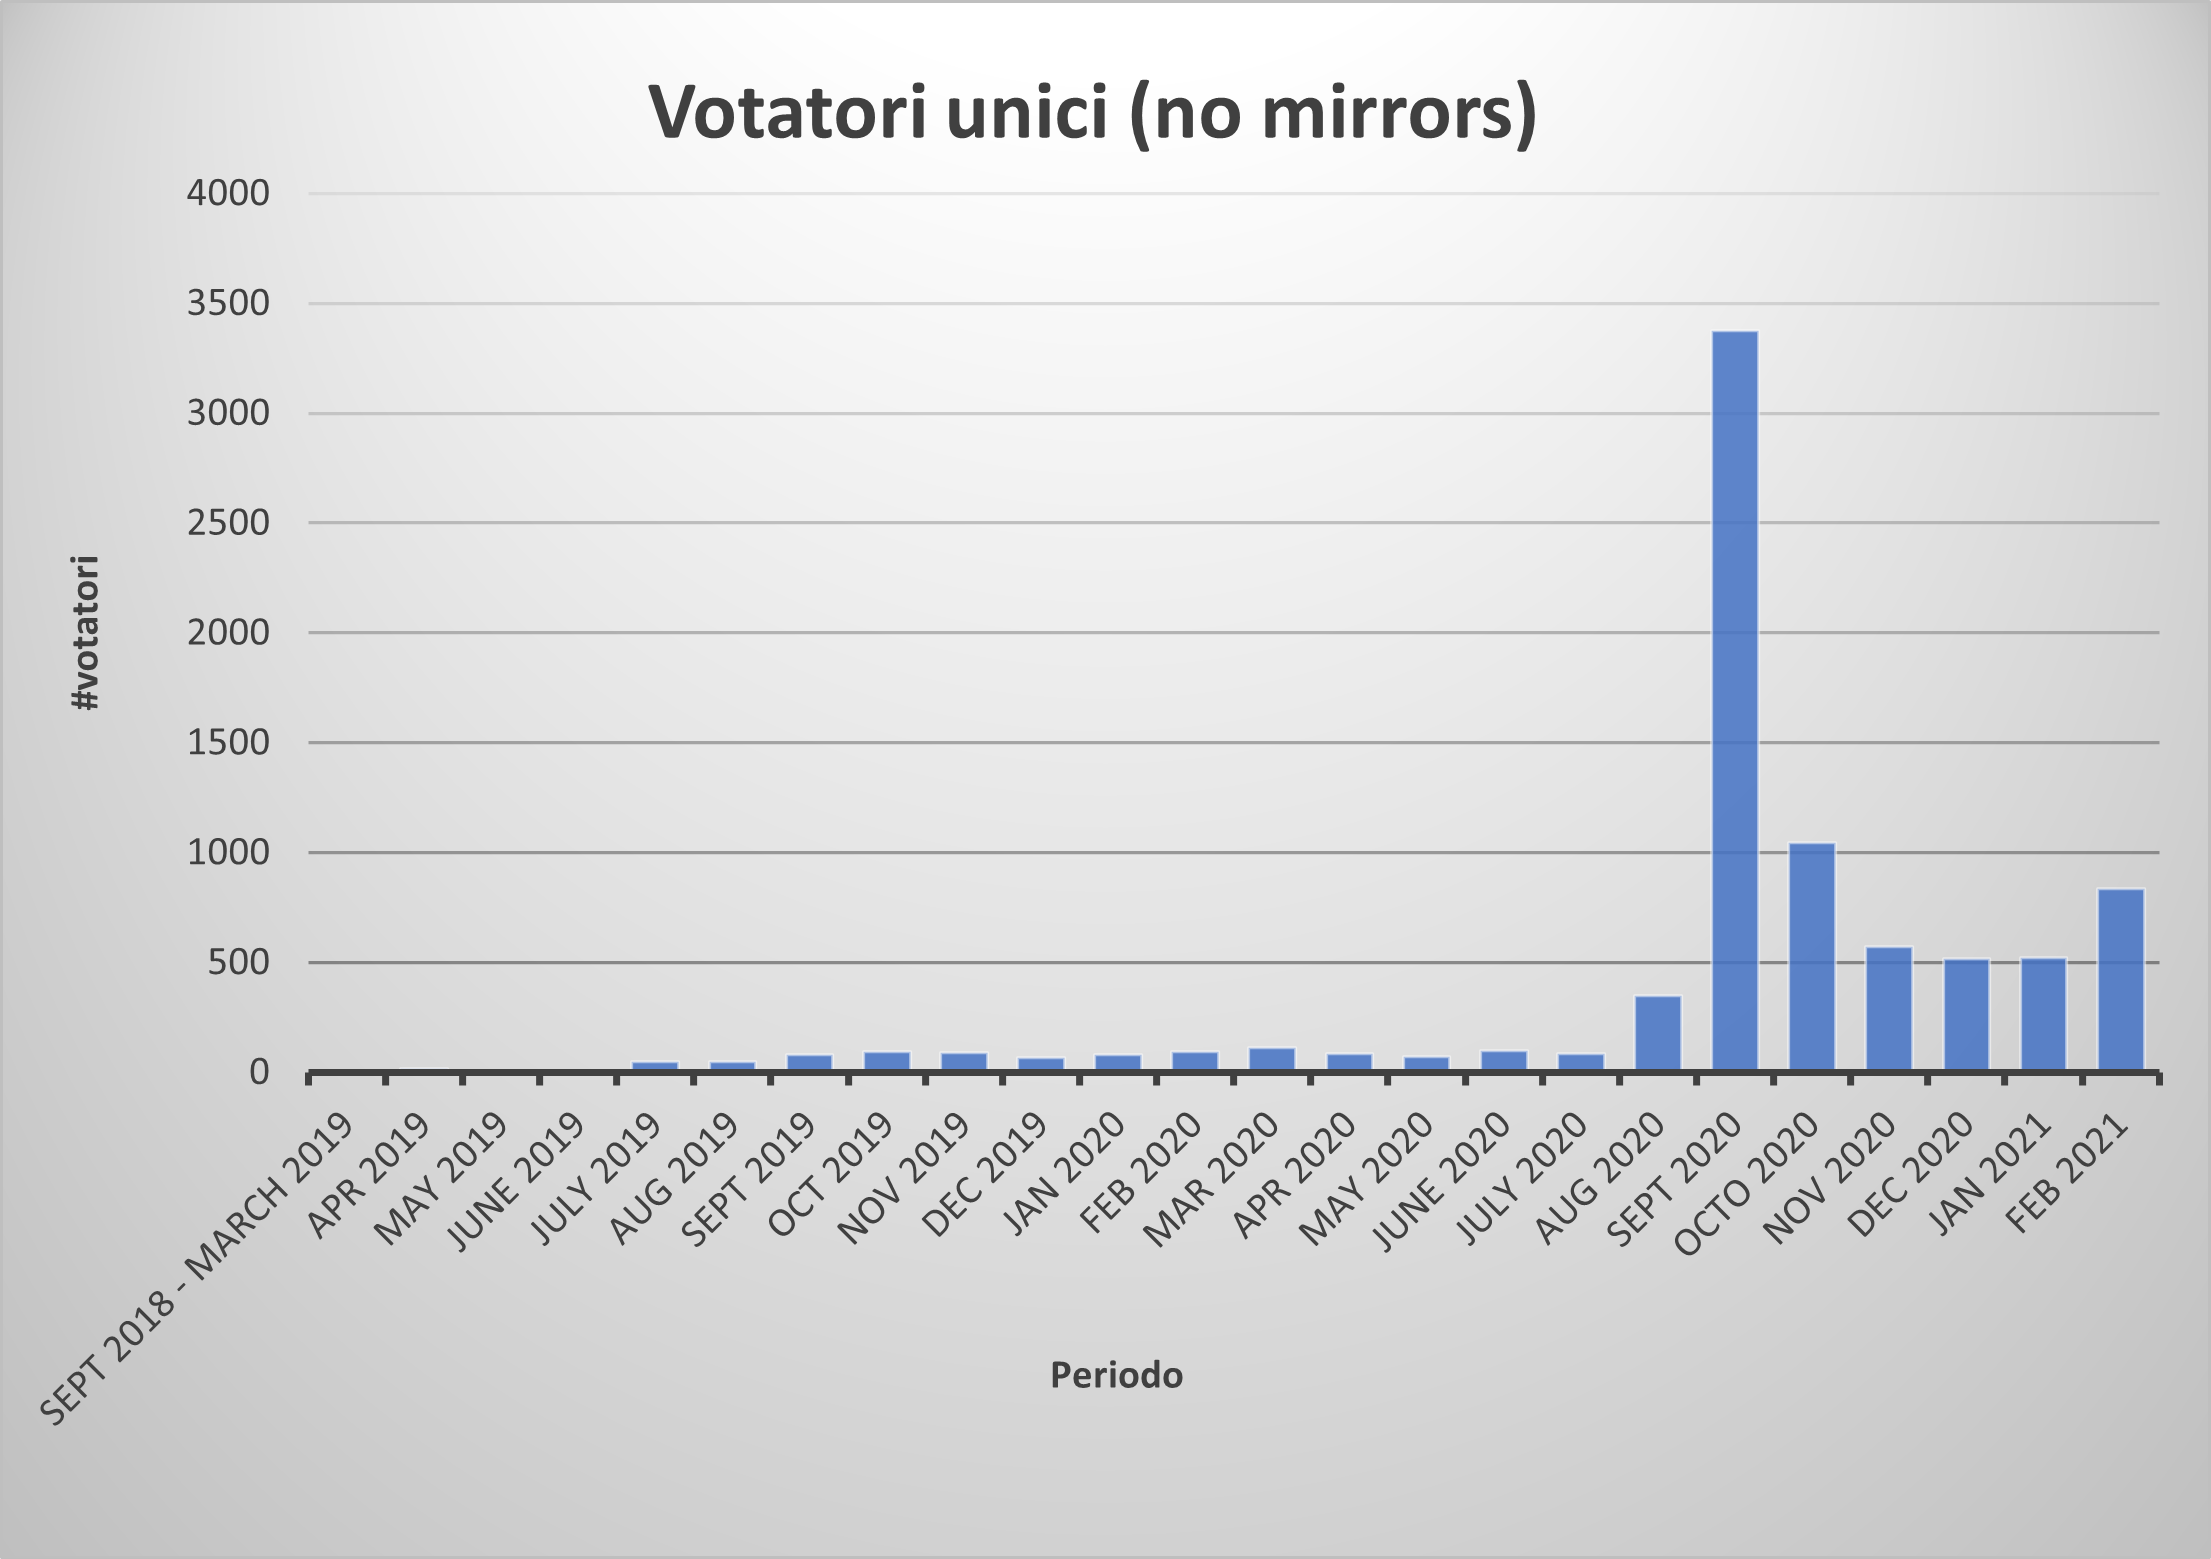
\includegraphics[width=.7\textwidth]{graphs/votatori_nomirr.png}
    \caption{Rappresentazione mensile dei votatori unici, solo account non-Mirror}
    \label{fig: uniquevoters_nomirr}
\end{figure}

Il grafico che considera solo account Mirror mostra che l'attività degli account Mirror ha subito un notevole decremento nel mese di Ottobre 2020, ovvero quando la fase Beta è ufficialmente terminata (Figura \ref{fig: uniquevoters_onlymirr}).
Ciononostante, l'attività dei Mirror è ricominciata a partire da Novembre 2020, e mostra una crescita costante.

Questo particolare si può osservare anche nella Figura \ref{fig: voting_onlymirr} che rappresenta, su base mensile, solo le azioni di voto effettuate da account Mirror. In questo caso abbiamo solo 5 azioni di voto nel mese di Ottobre 2020.

\begin{figure}[t]
    \centering
    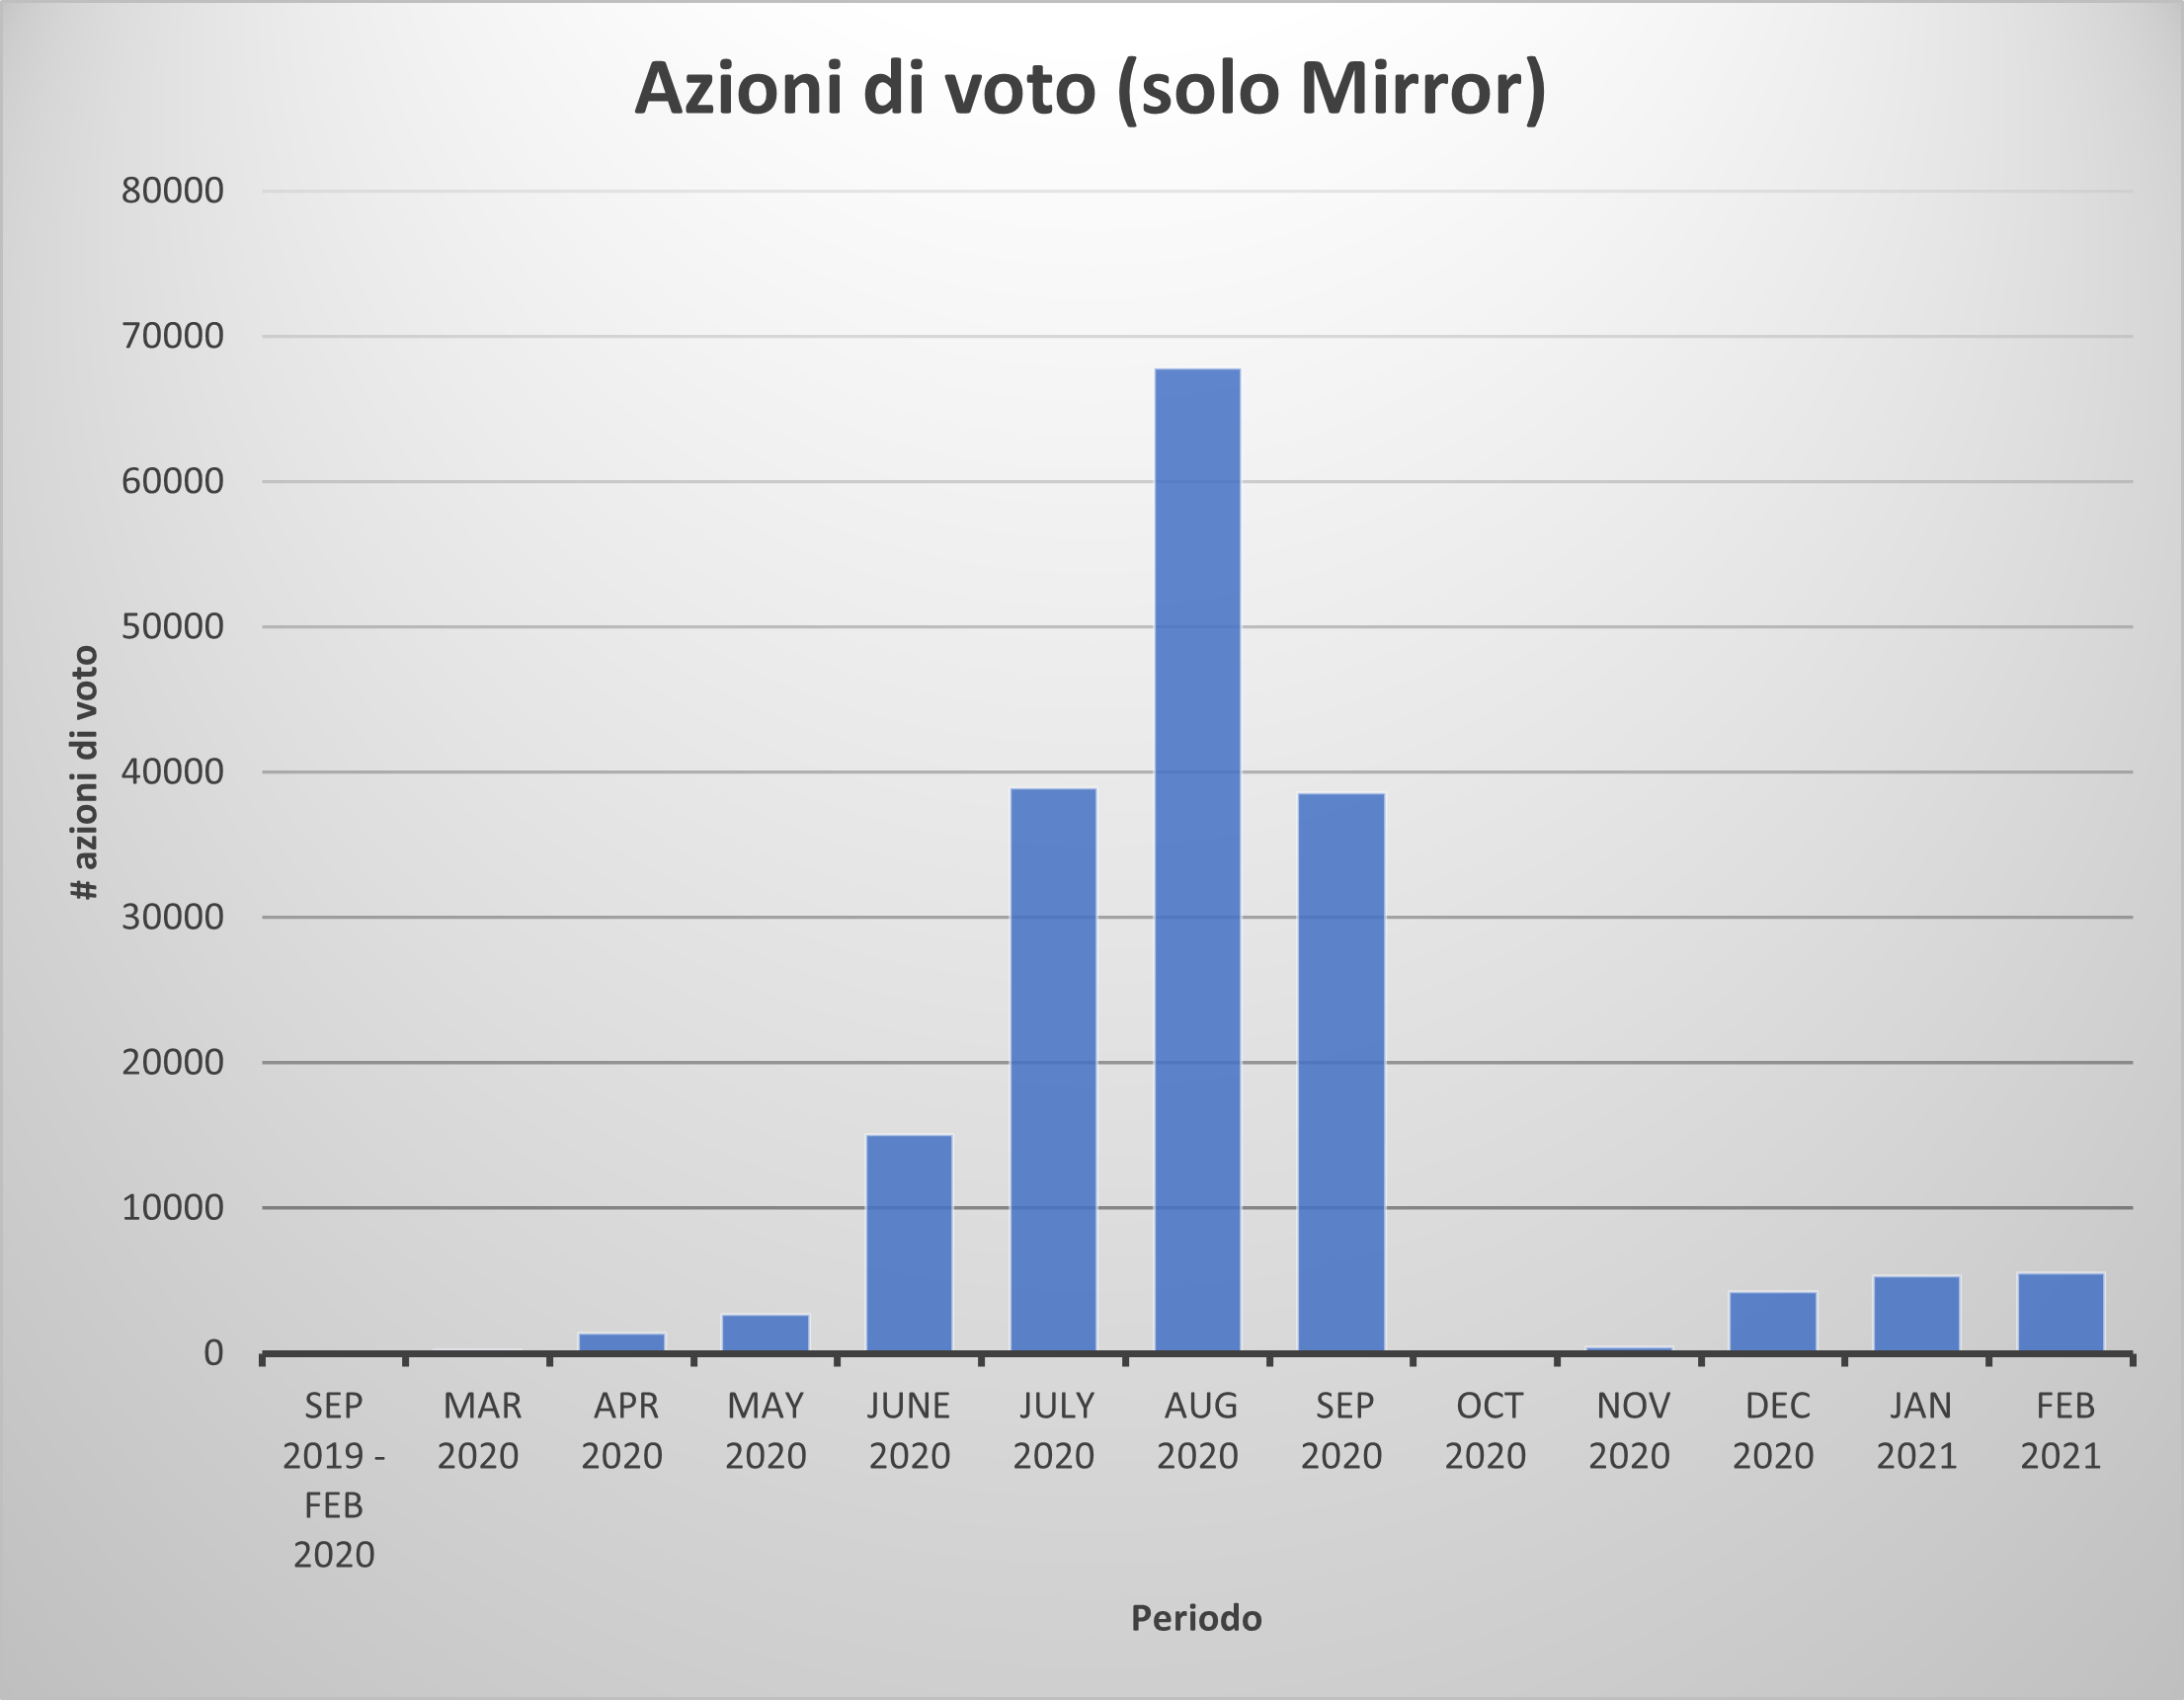
\includegraphics[width=.7\textwidth]{graphs/azioni_voto_onlymirr.png}
    \caption{Rappresentazione mensile delle azioni di voto, solo account Mirror}
    \label{fig: voting_onlymirr}
\end{figure}

Sembrerebbe che gli account Mirror inizialmente venissero ricompensati in qualità di creatori e successivamente questa funzionalità sia stata interrotta. Infatti le ultime ricompense assegnate ad account di questo tipo risalgono più o meno al mese di Luglio del 2020. Questo avvalora l'ipotesi che le ricompense creatore vengano momentaneamente accumulate sull'account \textbf{yupcreators1} con l'obiettivo di essere successivamente distribuite quando più creatori si "iscriveranno" effettivamente alla piattaforma.

\subsection{Distribuzione piattaforme}
\label{platoforms_section}
Ci concentriamo ora nello studio delle piattaforme i cui contenuti sono più comunemente votati su Yup.
Con lo scopo di effettuare un'analisi della distribuzione dei voti sulle varie piattaforme, da qui in poi considereremo solo le azioni di voto di account non-Mirror e per cui è stato possibile risalire al contenuto.
Esistono infatti alcuni casi in cui il postid relativo ad una createvote (link al voto antecedente in senso temporale) non era più presente all'interno del database, probabilmente perché il voto precedente è stato eliminato.
La scelta di concentrarci sui solo account non-Mirror deriva dal fatto di considerare azioni umane fatte sulla piattaforma, invece che considerare anche azioni non umane degli account Mirror.
Dalle nostre analisi, abbiamo individuato un numero di piattaforme uniche votate pari a \textbf{1.884}, che è un segno del fatto che utenti appartenenti a molte piattaforme sono interessate al concetto proposto da Yup.
\\
\\
In Figura \ref{fig: platformsunique_nomirr} mostriamo una rappresentazione delle piattaforme in cui sono stati votati il maggior numero di contenuti unici, mentre in Figura \ref{fig: platformstot_nomirr} mostriamo il numero di voti totali per i contenuti raggruppati per piattaforma.
Per una più facile comprensione dei grafici raggruppiamo in un'unica voce, \textbf{others}, i dati relativi alle piattaforme che non rientrano nelle 10 più importanti.

\begin{figure}[t]
    \centering
    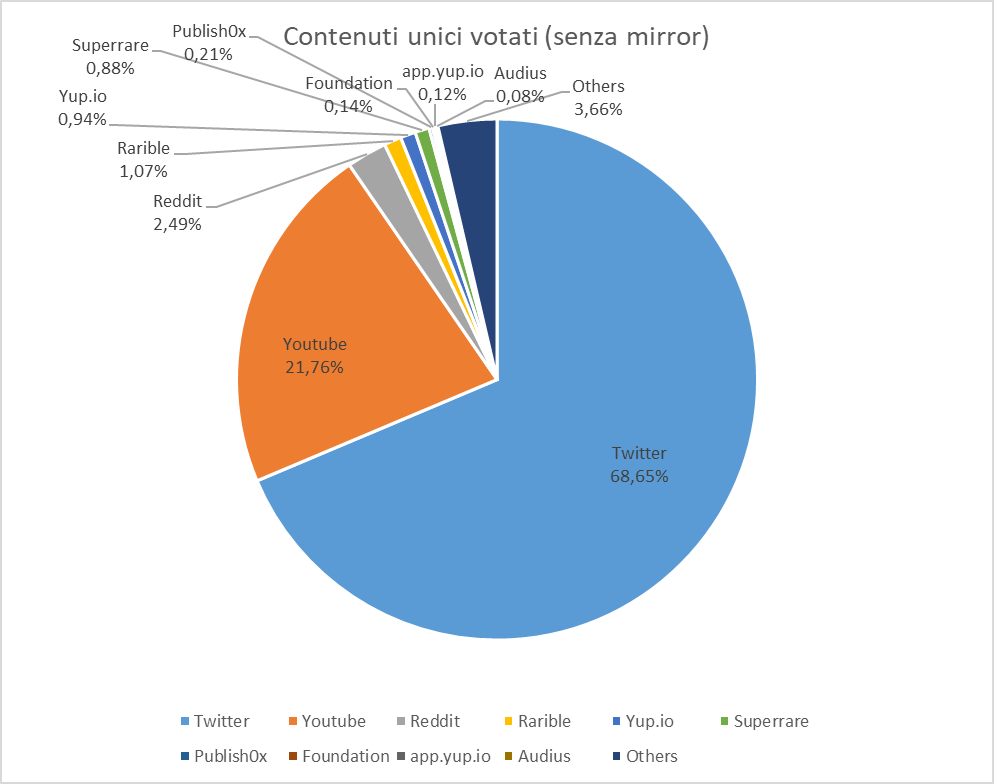
\includegraphics[width=0.7\textwidth]{graphs/platforms_unici_nomirr.png}
    \caption{Distribuzione dei contenuti votati sulle varie piattaforme escludendo account mirrors}
    \label{fig: platformsunique_nomirr}
\end{figure}    
    %\vspace*{\floatstep}
\begin{figure}[t]  
    \centering
    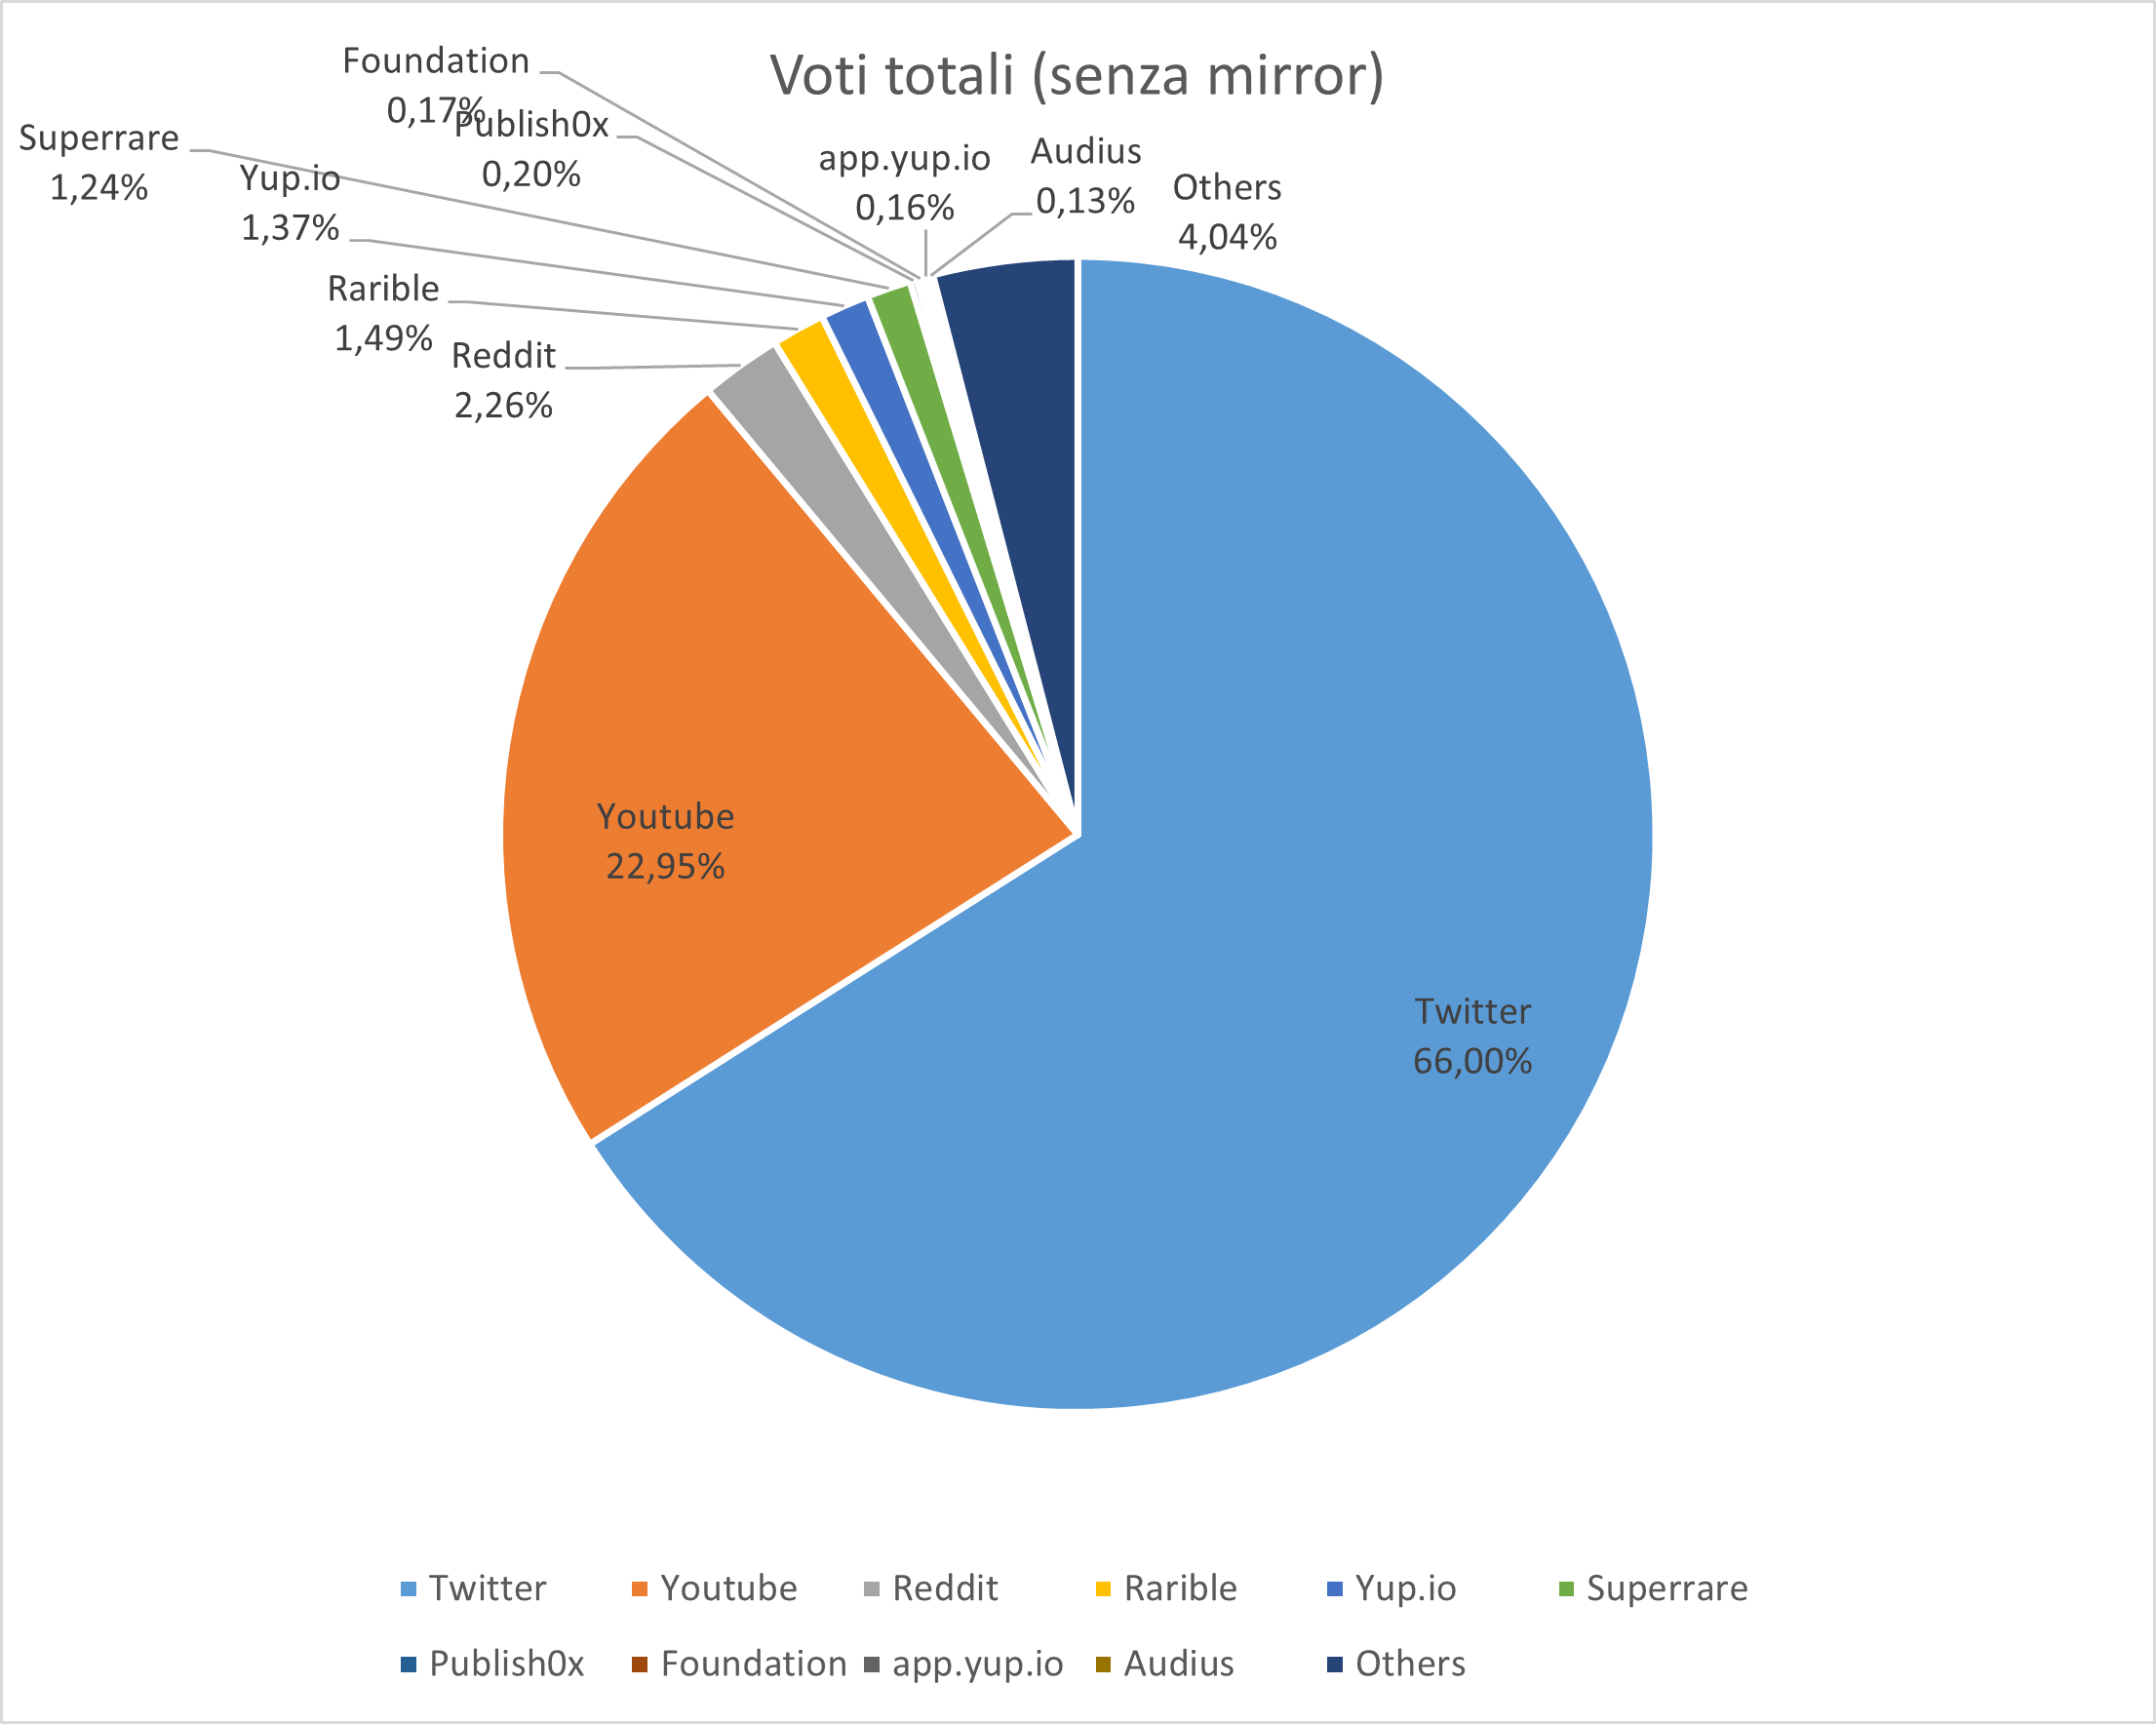
\includegraphics[width=0.7\textwidth]{graphs/platforms_tot_nomirr.png}
    \caption{Distribuzione dei voti totali sulle varie piattaforme escludendo account mirrors}
    \label{fig: platformstot_nomirr}
\end{figure}
%

Dalle Figure si può notare come le piattaforme integrate con l'estensione (Twitter, Youtube e Reddit) si trovino ai vertici della classifica. L'unica che costituisce una eccezione è Google Maps, la quale non compare nemmeno tra le 10 piattaforme più popolari. Continuando su questo aspetto, è interessante come siano presenti numerose piattaforme in ambito cripto, nonostante non supportino ancora l'overlay. In particolare, citiamo Rarible, Superrare e Foundation per quanto riguarda compravendita o in genere discussione su NFT; Publish0x è invece una piattaforma di blogging che ricompensa i propri utenti in criptovaluta e il cui sistema di ricompensa è basato su Ethereum; Audius, corrispettivo cripto di Spotify che distribuisce ricompense agli artisti, implementato su Ethereum.


Con l'obiettivo di avere risultati più specifici per i voti effettuati sulle principali piattaforme integrate, abbiamo indagato la distribuzione dei voti sui vari profili (Twitter), canali (Youtube) e subreddit (Reddit).
Questo ci permetterà di capire quali sono gli argomenti che catturano l'attenzione, ed in particolare i personaggi più seguiti, dagli utenti di Yup.
Mostriamo in Tabella \ref{tab: profiles_votes} il numero di profili Twitter, canali Youtube e subreddit votati almeno una volta da utenti Yup.

\begin{table}[h!]
\centering
\begin{tabular}{ |c|c|}
\hline
PROFILI TWITTER & 29.880 \\
\hline
CANALI YOUTUBE & 3.897 \\
\hline
SUBREDDITS & 628 \\
\hline
\end{tabular}
\caption{Profili unici votati}
\label{tab: profiles_votes}
\end{table}

In particolare notiamo come i profili Twitter siano di gran lunga più comune, probabilmente grazie alla notorietà della piattaforma e alla possibilità di includere in un singolo contenuto (tweet) testo, immagini, link e video.

Di seguito mostriamo i grafici del numero di voti dei 10 profili Twitter più votati (Figura \ref{fig: twitter_profiles}), dei 10 canali Youtube più votati (Figura \ref{fig: youtube_channels}) e dei 10 subreddit più votati \ref{fig: reddit_subreddits}. Anche in questo caso mostriamo solamente i 10 account con maggior numero di voti per motivi di comprensione e includiamo i dati di tutti gli elementi restanti in \textbf{others}.

\begin{figure}[t]
    \centering
    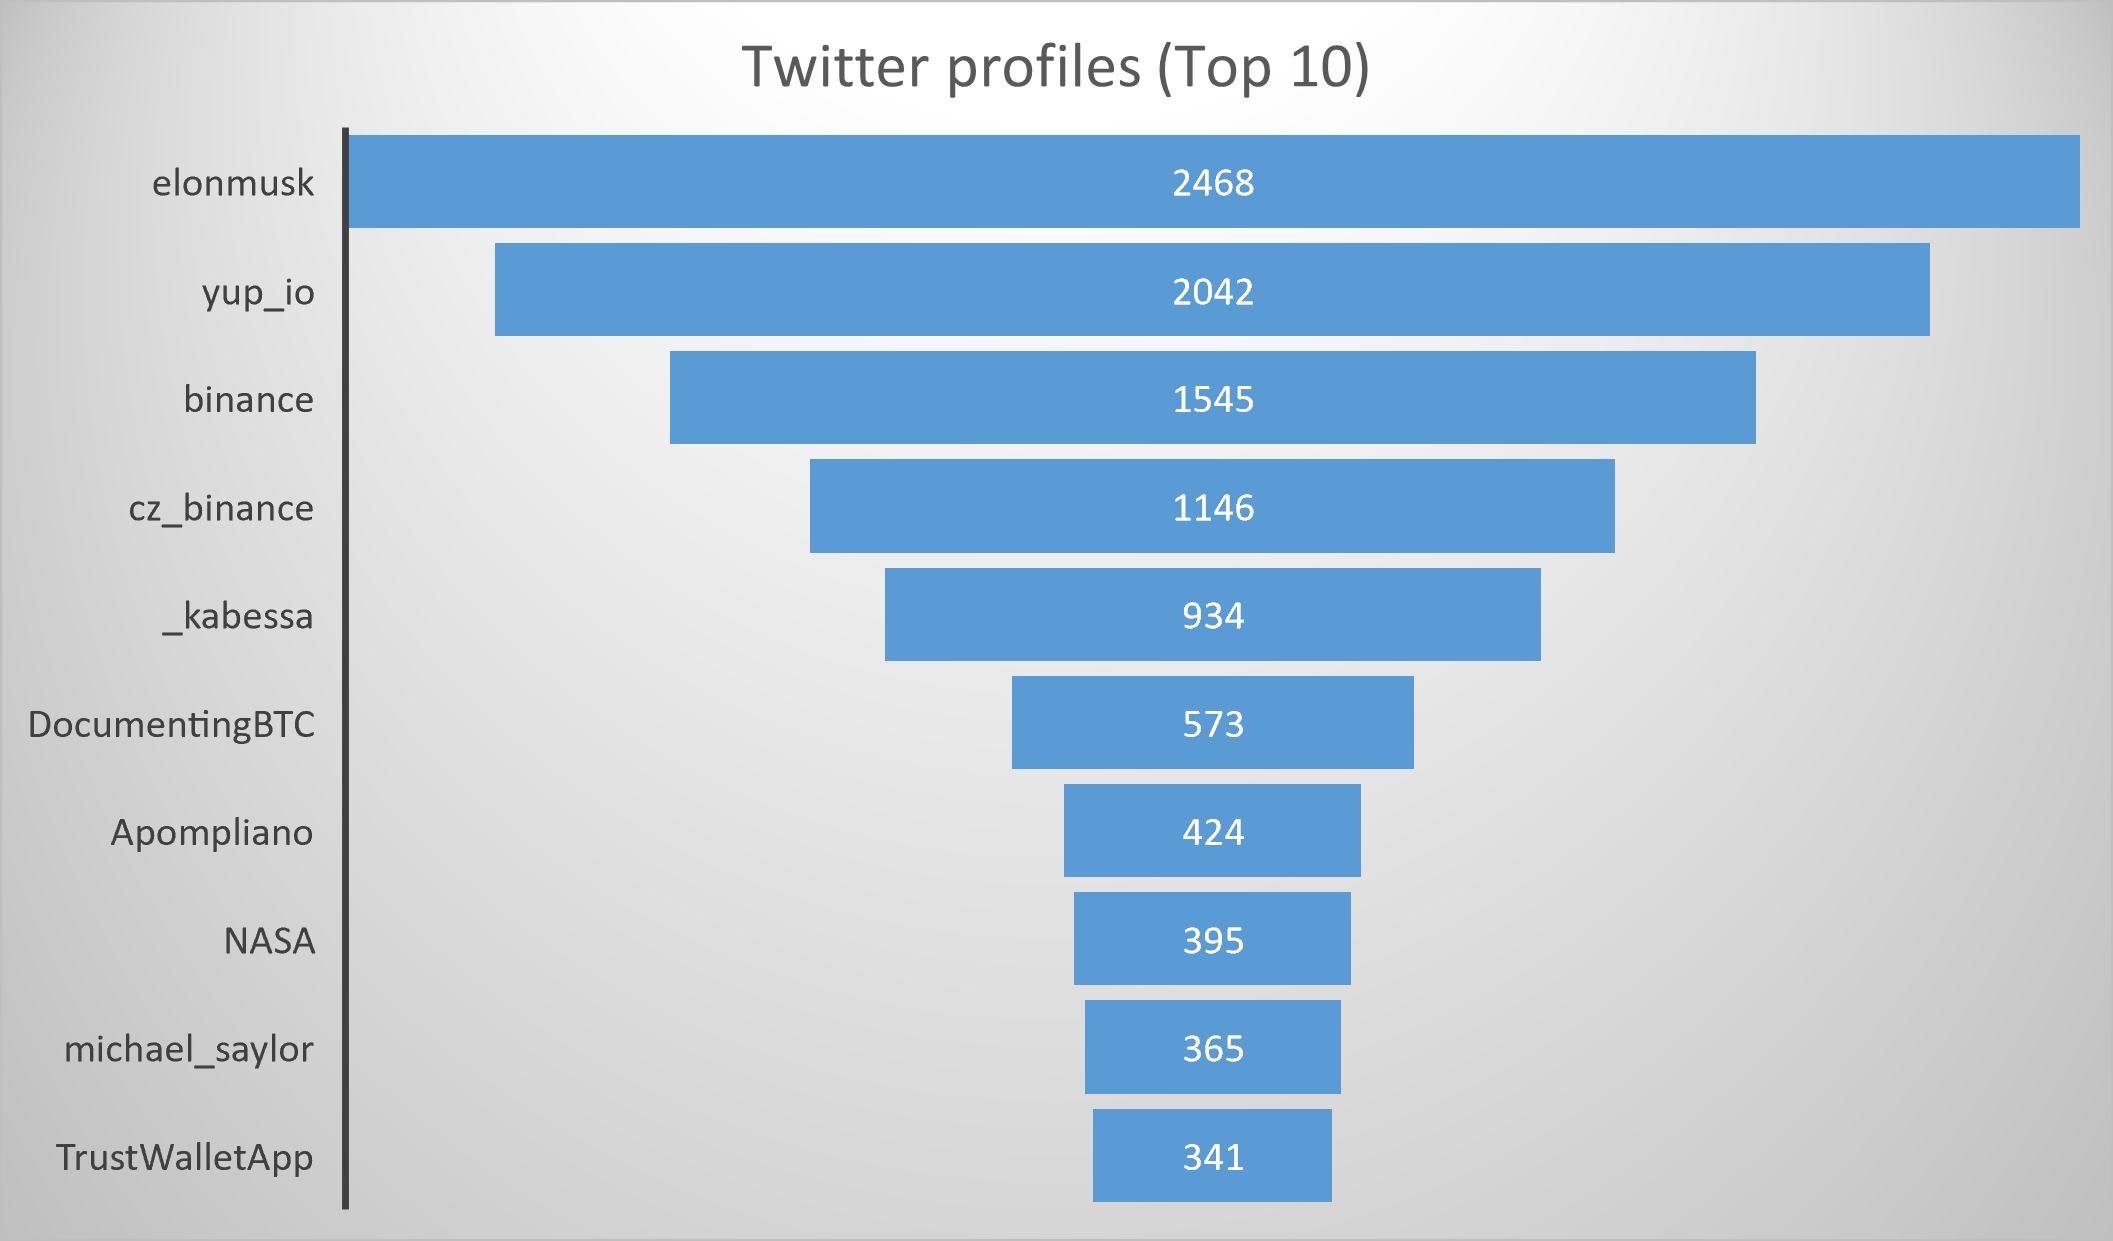
\includegraphics[width=0.8\textwidth]{graphs/twitter_profiles.png}
    \caption[twitter profiles]{Top 10 profili Twitter con più voti totali
    \\
    \centering
    \begin{itemize}
        \centering
        \item \textbf{VOTI TOTALI TWITTER:} 121.876
        \item \textbf{others:} 111.643
    \end{itemize}}
    \label{fig: twitter_profiles}
\end{figure}

Nel caso di Youtube è stato considerato un sottogruppo dei dati di partenza, abbiamo infatti tenuto conto dei soli video che avevano ricevuto più di un voto. Questo perché la quantità di voti era difficilmente trattabile, per via del limit rate imposto dalle API della piattaforma, necessarie per reperire il nome del canale Youtube partendo dal link del video votato. Inoltre aumentiamo la possibilità di escludere potenziali self-voters: questi non vengono infatti eliminati del tutto con il criterio utilizzato poiché, come già spiegato nel Capitolo \ref{platform_chapter}, è possibile effettuare fino a 3 voti sullo stesso contenuto cambiando la categoria.

\begin{figure}[t]
    \centering
    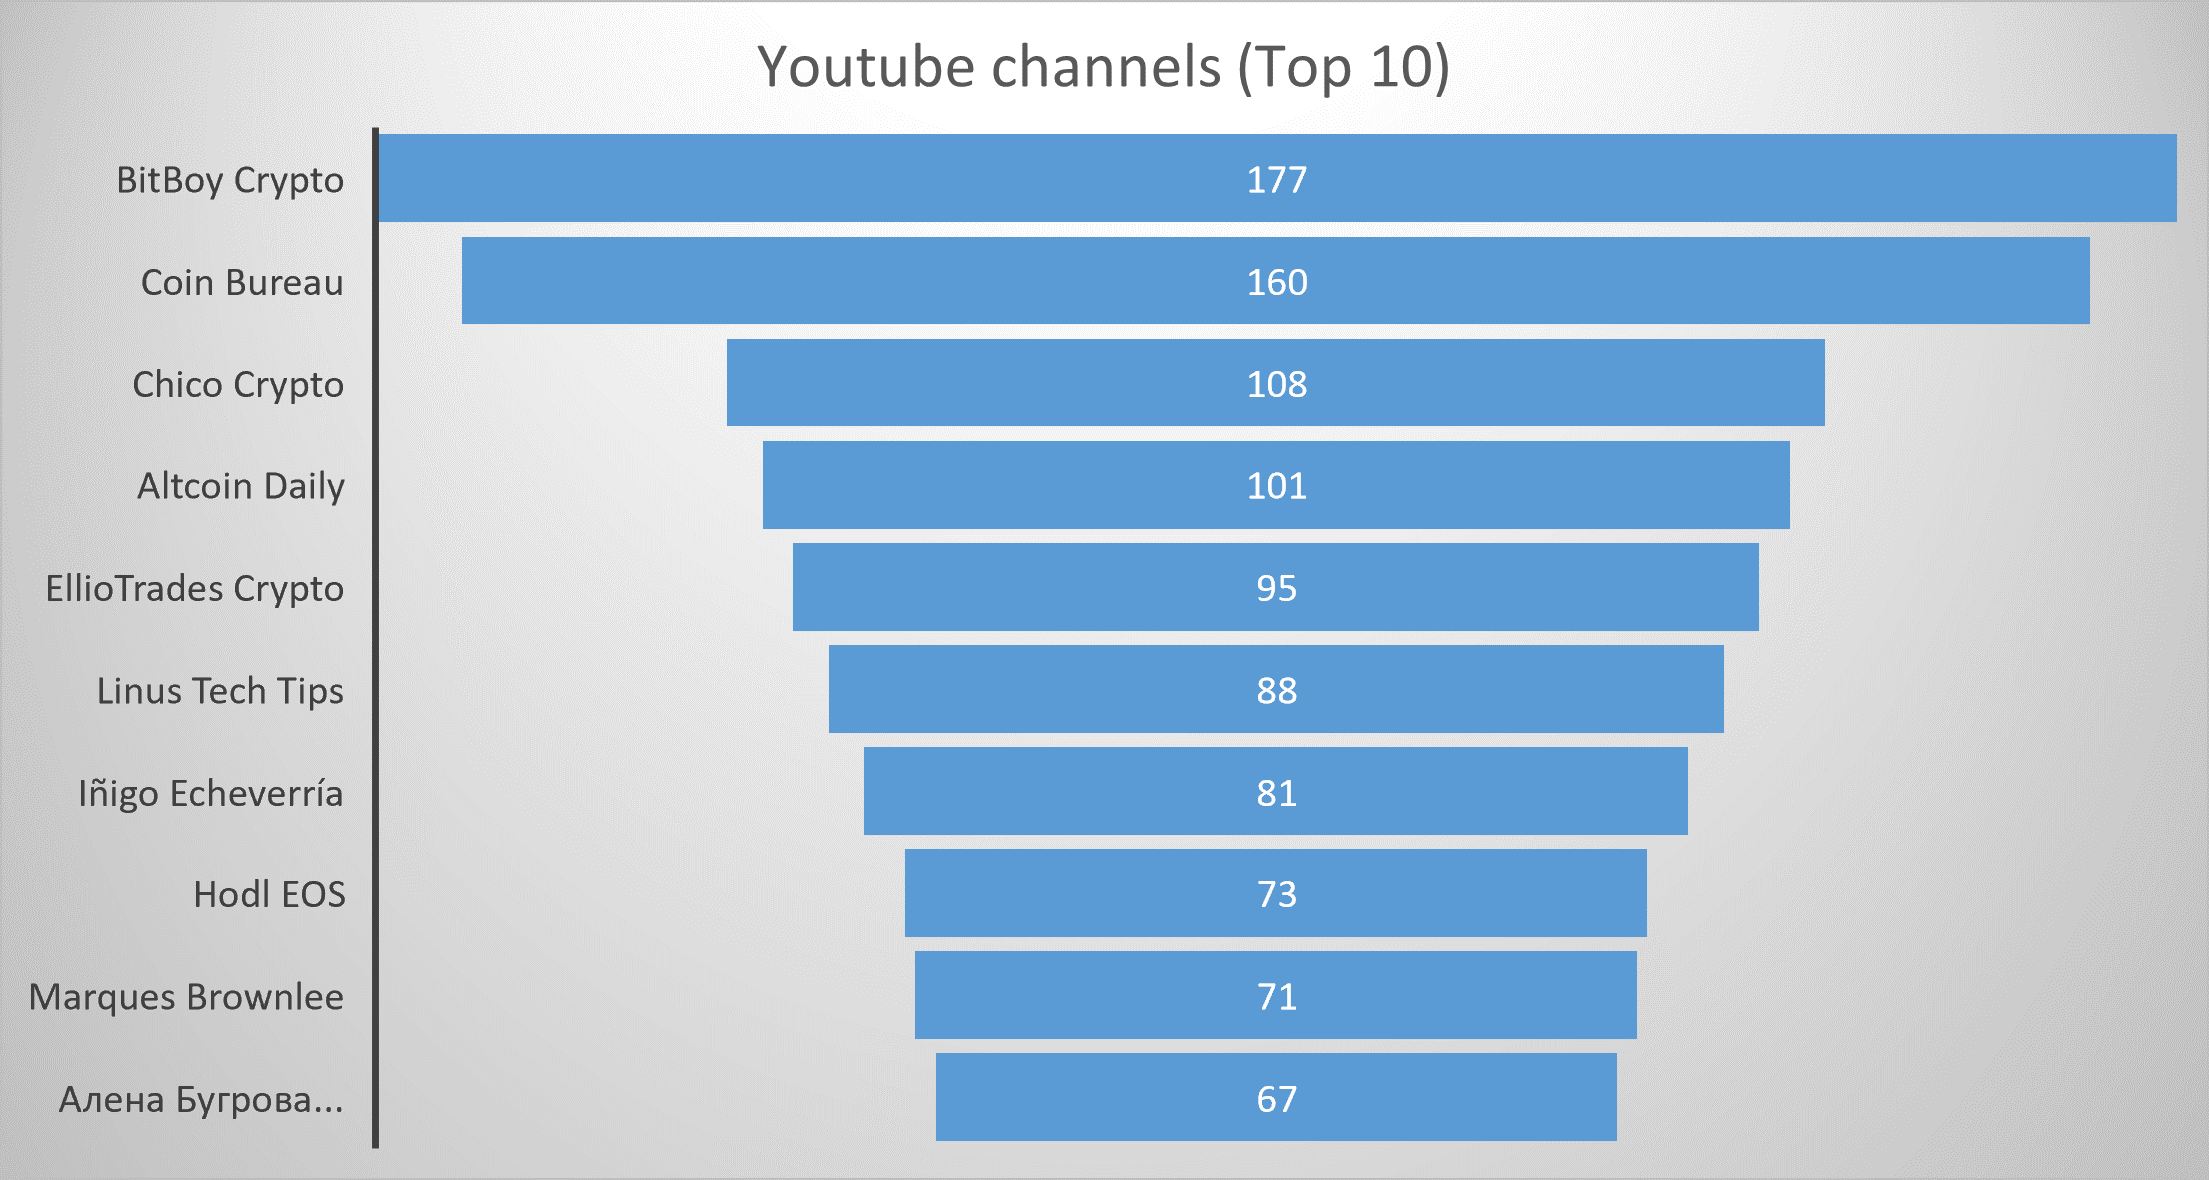
\includegraphics[width=0.7\textwidth]{graphs/youtube_channels.png}
    \caption[youtube channels]{Top 10 canali Youtube con più voti totali
    \\
    \centering
    \begin{itemize} \centering
        \item \textbf{VOTI TOTALI YOUTUBE:} 16.169
        \item \textbf{others:} 15.148
    \end{itemize}}
    \label{fig: youtube_channels}
\end{figure}

\begin{figure}[t]
    \centering
    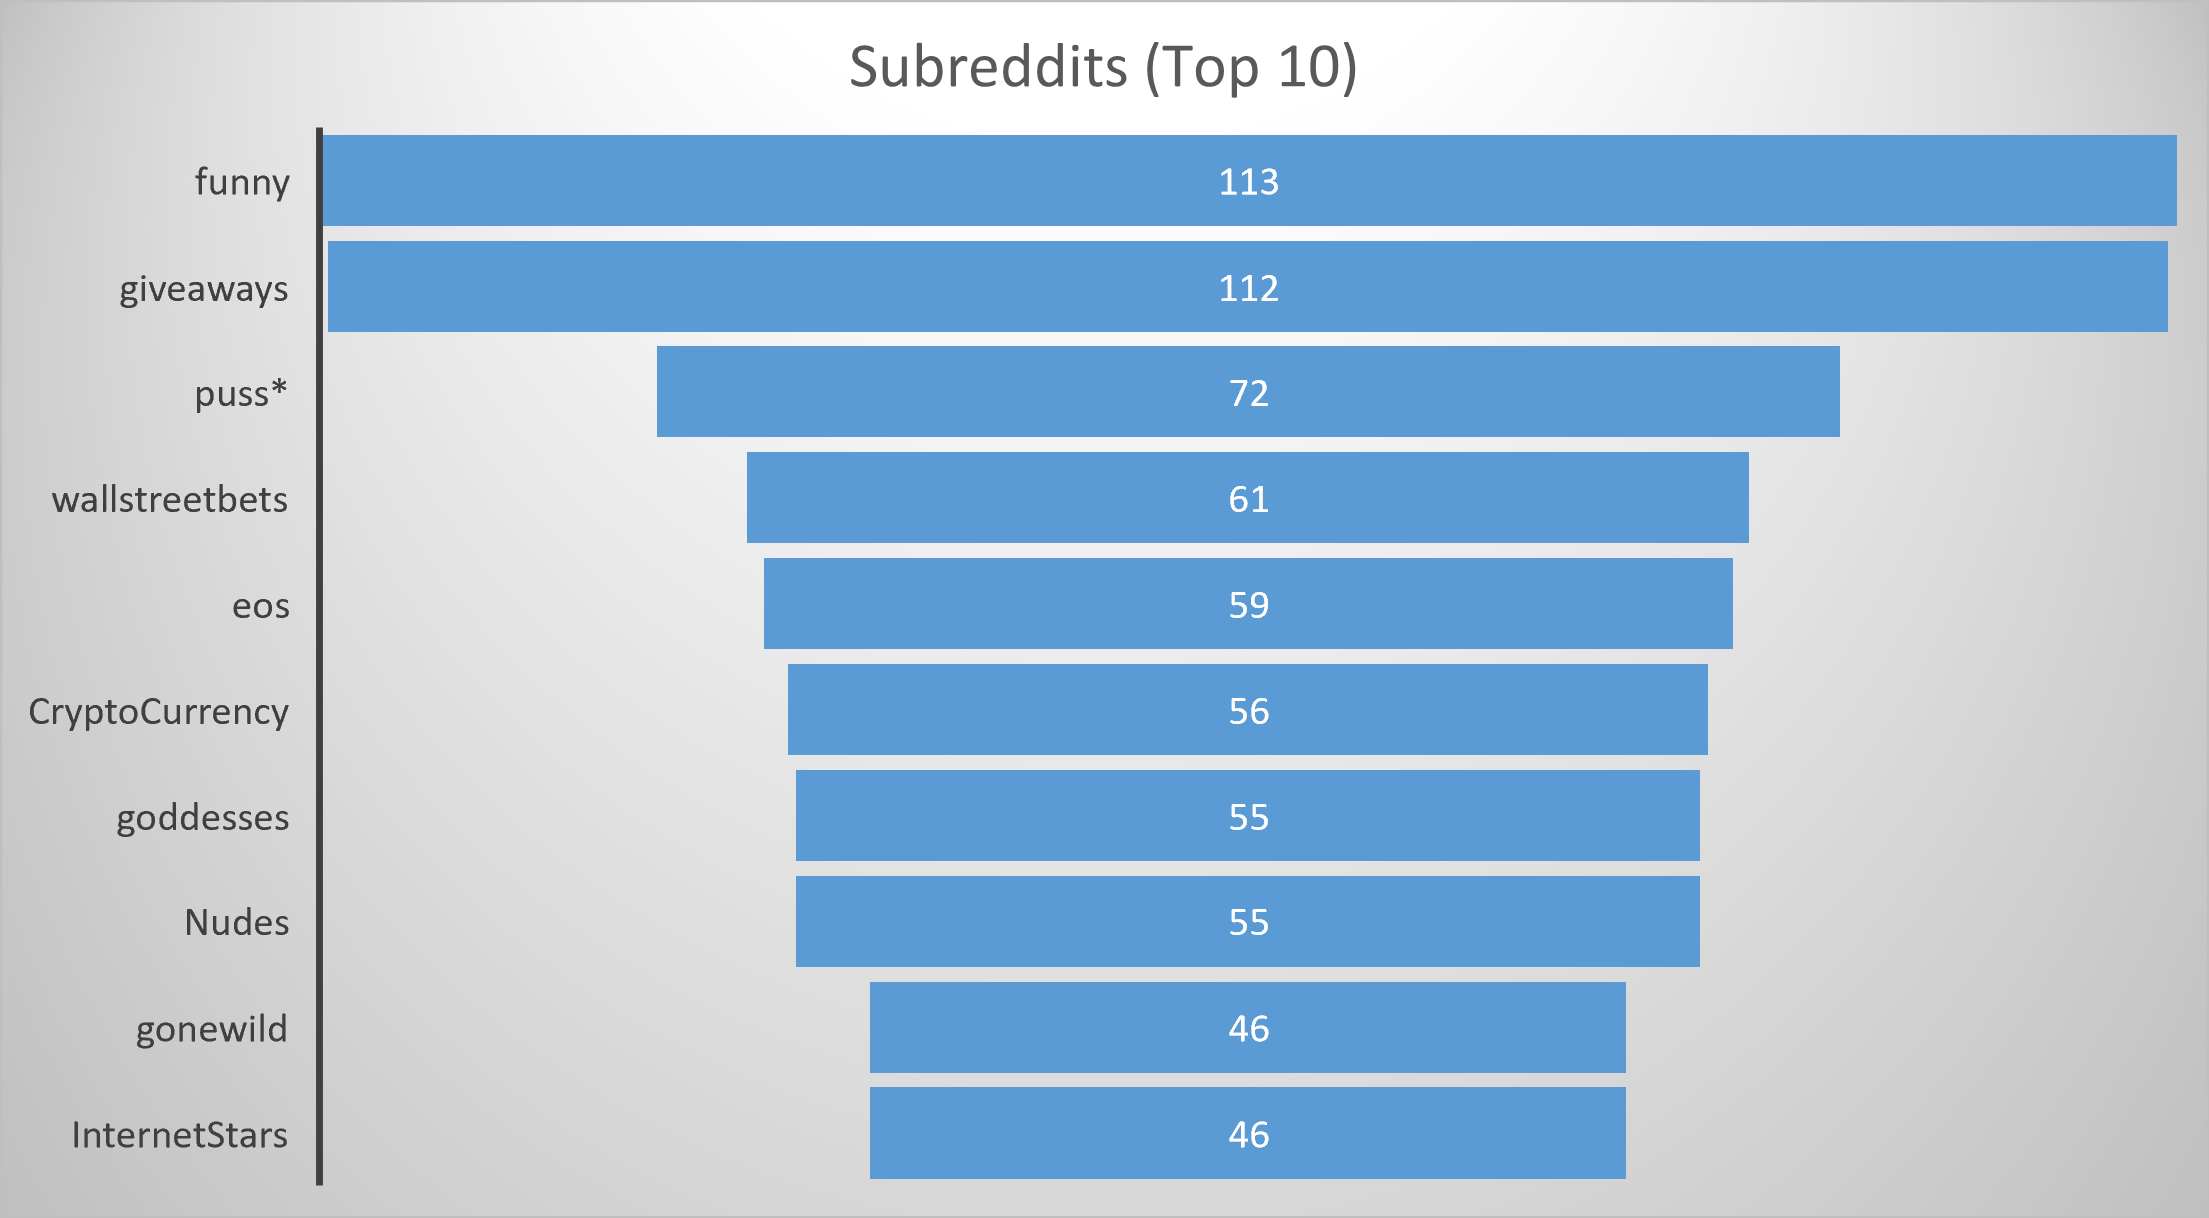
\includegraphics[width=0.7\textwidth]{graphs/subreddits.png}
    \caption[subreddits]{Top 10 subreddit di Reddit con più voti totali
    \\
    \centering
    \begin{itemize} \centering
        \item \textbf{VOTI TOTALI REDDIT:} 3.499
        \item \textbf{others:} 2.824
    \end{itemize}}
    \label{fig: reddit_subreddits}
\end{figure}


Osservando le 3 Figure, relative alle tre piattaforme più votate con Yup, il primo fatto che salta subito all'occhio è che la maggior parte dei voti venga attribuita ad individui o a gruppi che trattano o sono vicini al mondo cripto. 


Nel caso dei profili Twitter maggiormente votati è anche osservabile come siano presenti o individui di elevata notorietà in tale ambito (Elon Musk, CZ Binance, APompliano) o il profilo ufficiale di Yup (Yup.io) e quelli di alcuni developer (\_Kabessa).
Similmente, tra i canali Youtube più popolari troviamo quasi esclusivamente appassionati di criptovalute o altri canali dove si trattano argomenti tecnici legati alla tecnologia blockchain.
Su Reddit la situazione è più eterogenea, infatti troviamo subreddit legati a criptovalute (eos e CryptoCurrency), investimenti (wallstreetbets), ma anche alcuni subreddit con materiale NSFW (puss*, goddesses, Nudes, gonewild, InternetStars).

La forte attenzione riguardo al mondo delle criptovalute e delle blockchain in generale è un risultato atteso se, ricordando che le ricompense di un utente dipendono dal numero di voti che occorrono dopo il suo, pensiamo a come sia più probabile avere guadagni maggiori votando account molto seguiti o appartenenti a personaggi eccentrici, come Elon Musk, oppure anche account con meno seguaci ma la cui esposizione ad utenti Yup è intuitivamente significativa, come l'account ufficiale della dApp.
Questo ci porta inoltre a pensare che ci sia una certa polarizzazione nei contenuti maggiormente monitorati dagli utenti.
Questo fenomeno potrebbe ulteriormente amplificarsi nel tempo.
Infatti se i nuovi utenti saranno solamente interessati a generare profitto, la loro migliore strategia per generarne il più possibile sarebbe quella di sfruttare l'estrema popolarità di questi account ed esprimere un voto il prima possibile, andando ad invalidare le premesse della piattaforma.
D'altro canto questo risultato, unito a quello della distribuzione dei voti per piattaforma, potrebbe essere invece segnale che l'utenza che utilizza il servizio, almeno per il momento, sia prevalentemente di nicchia.
Un risultato naturale se si pensa che sia più probabile che persone interessate a questi argomenti abbiano sentito parlare di Yup e di conseguenza si siano iscritti. 


\subsection{Distribuzione utenti-piattaforme}
Ci siamo infine concentrati sulla possibilità che un utente possieda o meno un account su altri social network. Ricordiamo infatti che su ogni piattaforma, anche se non integrata sull'applicazione ufficiale di Yup, è possibile esprimere la valutazione di un contenuto e registrare la valutazione sullo smart contract EOS d Yup. Nel nostro studio abbiamo selezionato solo alcune piattaforme tra quelle più famose anche non nel mondo cripto: Twitter, Youtube, Facebook, Reddit, Instagram, Spotify. Di seguito indichiamo, per ognuna di queste piattaforme, il numero di utenti che ne hanno votato almeno un contenuto:

\begin{itemize}
    \item \textbf{TWITTER}: 2.272
    \item \textbf{YOUTUBE}: 2.379
    \item \textbf{REDDIT}: 307
    \item \textbf{FACEBOOK}: 80
    \item \textbf{INSTAGRAM}: 39
    \item \textbf{SPOTIFY}: 44
\end{itemize}

Twitter e Youtube si confermano le piattaforme social più popolari dal punto di vitsta della votazione, ma notiamo che il numero di utenti che ha votato almeno un contenuto Youtube è leggermente superiore al numero di utenti che ha votato almeno un contenuto su Twitter.
Se consideriamo che il numero di voti espressi su Twitter (Figura \ref{fig: twitter_profiles}) è circa 7.5 volte il numero di voti espressi su Youtube (Figura \ref{fig: youtube_channels}), possiamo anche concludere che spesso su Youtube si esprimono pochi voti.

Partendo da questi dati abbiamo anche effettuato un'intersezione tra gli insiemi di utenti che hanno votato le piattaforme considerate, ottenendo un totale di \textbf{3.232 votatori unici} (sono 5.121 gli utenti che hanno espresso almeno un voto). Riportiamo la distribuzione del numero di utenti per il numero di piattaforme votate:

\begin{itemize}
    \item \textbf{6/6}: 4
    \item \textbf{5/6}: 12
    \item \textbf{4/6}: 42
    \item \textbf{3/6}: 254
    \item \textbf{2/6}: 1.187
    \item \textbf{1/6}: 1.733
\end{itemize}

Questa distribuzione ci suggerisce che sono pochi gli utenti che utilizzano Yup al pieno del suo potenziale e che in genere si preferisce concentrarsi su al più due piattaforme. 

Da questo studio tuttavia non si ha la certezza che un individuo possieda un account su una determinata piattaforma, anche nel caso in cui per visualizzare un contenuto e quindi votarlo sia necessario il login (per esempio su \textbf{Instagram} o \textbf{Facebook}).
Questo succede perché, tramite l'interfaccia di Yup.io, è possibile esprimere opinioni in maniera "indiretta", ispezionando l'attività di altri utenti. Per esempio un utente può votare un contenuto relativo a Facebook che è stato votato da un altro utente accedendo al suo profilo e votandolo sulla piattaforma.


Con l'idea di ottenere risultati più accurati riguardo il fatto di possedere un account su una delle piattaforme studiate, è stata ripetuta la stessa analisi considerando solo gli utenti che sono stati i primi a votare (studiando quindi le azioni della famiglia postvote).
Grazie a questa analisi, almeno per quelle piattaforme in cui il login è obbligatorio, (Youtube, Reddit, e Twitter sono fanno eccezione ma riportiamo comunque i loro dati per completezza), il voto è stato necessariamente effettuato in maniera "diretta", ovvero visualizzando il contenuto sulla piattaforma social e votando tramite overlay Yup, e quindi il votatore deve esservi registrato.

\begin{itemize}
    \item \textbf{TWITTER}: 1.402
    \item \textbf{YOUTUBE}: 1.109
    \item \textbf{REDDIT}: 187
    \item \textbf{FACEBOOK}: 43
    \item \textbf{INSTAGRAM}: 26
    \item \textbf{SPOTIFY}: 21
\end{itemize}

%Categorie: spostata in YupPlatform

%Account Mirror: spostata sopra in trattazione figure dei solo Mirror

\section{Utilizzo del Bridge}
Passiamo ora allo studio del bridge, ovvero la componente che serve per gestire il flusso di criptovaluta e l'interazione tra le blockchain di EOS e Ethereum.
Di seguito riportiamo un'analisi che ha l'obiettivo, considerando esclusivamente i trasferimenti di token verso Ethereum (quindi un "prelievo" di YUP) e quelli relativi al pagamento delle corrispondenti tasse, di dare un'idea di quanto nell'utenza abbia guadagnato tramite l'utilizzo del servizio e di quanto abbia perso per via delle tasse legate al Bridge. Abbiamo escluso quei trasferimenti effettuati da \textbf{yupaccounts1} e \textbf{testpoolbox1} poiché transazioni atte a testare il Bridge al momento della sua introduzione, di fatto hanno effettuato i primi trasferimenti e non compaiono più successivamente.


Le azioni che si occupano del trasferimento dei token verso l'indirizzo Ethereum dell'utente (riportato nel campo \textbf{memo} dell'azione) hanno come destinatario dell'azione EOS \textbf{bridge.yup}. Questo perché viene adottato un approccio \textbf{mint-burn} (descritto nell'apposita sezione Bridge nel \textbf{Capitolo 3}), ovvero i token non vengono realmente spostati dalla blockchain, ma vengono "bruciati" su EOS e creati su Ethereum. Mostriamo in Tabella \ref{tab: bridge_analytics} alcuni dati di analisi tenendo in considerazione solo i transfer verso indirizzi Ethereum e in Figura \ref{fig: top10_bridge} gli utenti che hanno spostato la maggior quantità di token.


\begin{table}[h]
\centering
\begin{tabular}{ |c|c|}
 \hline
 TRASFERIMENTI DI TOKEN SU ETH & 334 \\
 \hline
 TOKEN MIGRATI SU ETH & 119.024,47 YUP \\
 \hline
 MASSIMO BRIDGE & 24.950 YUP \\
 \hline
 MINIMO BRIDGE & 0,001 YUP \\
 \hline
 MEDIA BRIDGE & 356,36 YUP \\
 \hline
\end{tabular}
\caption{Dati analitici dell'utilizzo del Bridge}
\label{tab: bridge_analytics}
\end{table}

La Tabella ci mostra che l'utilizzo del bridge è limitato a poche centinaia di transazioni, e quindi poco comune su Yup se comparato al altre attività, come il voto.
Ciononostante, notiamo che oltre 100.000 token sono stati trasferiti da EOS a Ethereum, probabilmente perché Ethereum ospita molte dapp e il mercato di compravendita di token su Ethereum è molto più florido, rendendo quindi i token più facilmente scambiabili.

\begin{figure}[t]
    \centering
    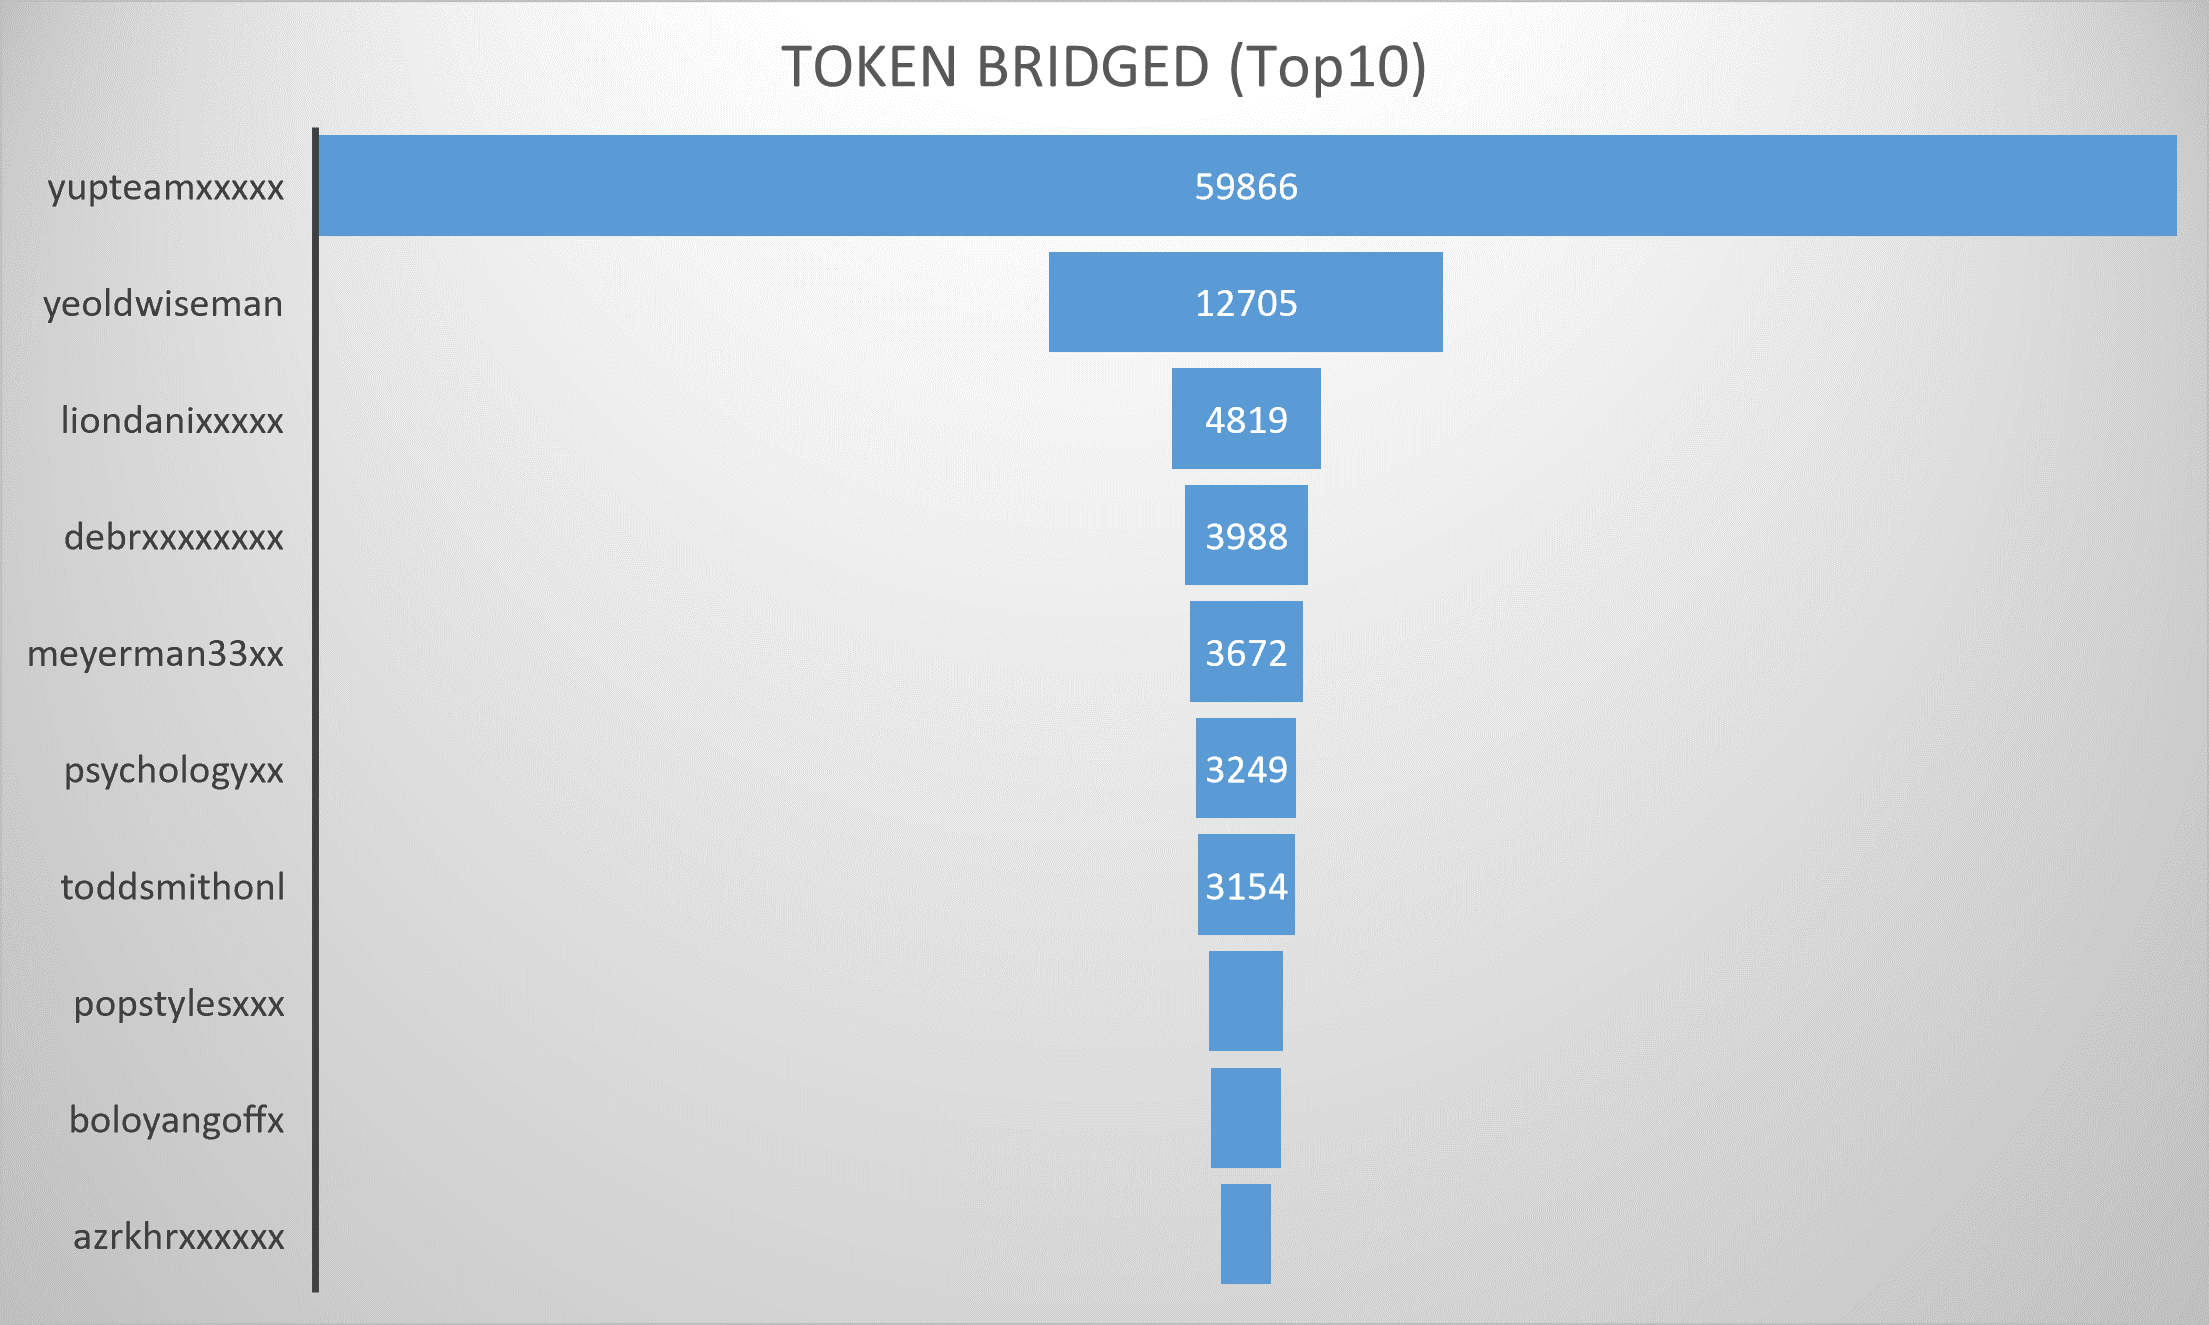
\includegraphics[width=.7\textwidth]{graphs/top10_bridge.png}
    \caption{Top 10 degli account che hanno trasferito la maggior quantità di token su Ethereum}
    \label{fig: top10_bridge}
\end{figure}

Dalla Figura possiamo invece osservare come l'account \textit{yupteamxxxxx} sia di gran lunga quello ad aver migrato più token sulla blockchain di Ethereum (Figura \ref{fig: top10_bridge}). Quest'ultimo raggruppa tutte le ricompense che, secondo quanto descritto nella documentazione della piattaforma, sono destinate ai membri del team.

Le azioni che si occupano del trasferimento dei token in qualità di tassa sono invece rivolte verso \textbf{yupaccounts1}. Mostriamo in Tabella \ref{tab: fees_analytics} alcuni dati di analisi tenendo in considerazione solo i transfer in quanto pagamento della tassa del Bridge e in Figura \ref{fig: top10_fees} gli utenti che hanno "speso" la maggior quantità di token per via della tassa sul trasferimento all'account bridge.

\begin{table}[h!]
\centering
\begin{tabular}{ |c|c|}
 \hline
 TRASFERIMENTI DI TASSE & 333 \\
 \hline
 TOKEN PERSI IN TASSE & 2.781,79 YUP \\
 \hline
 MASSIMA TASSA PAGATA & 62,45 YUP \\
 \hline
 MINIMA TASSA PAGATA & 0,18 YUP \\
 \hline
 MEDIA TASSA & 8,35 YUP \\
 \hline
\end{tabular}
\caption{Dati analitici delle tasse del Bridge}
\label{tab: fees_analytics}
\end{table}

\begin{figure}[t]
    \centering
    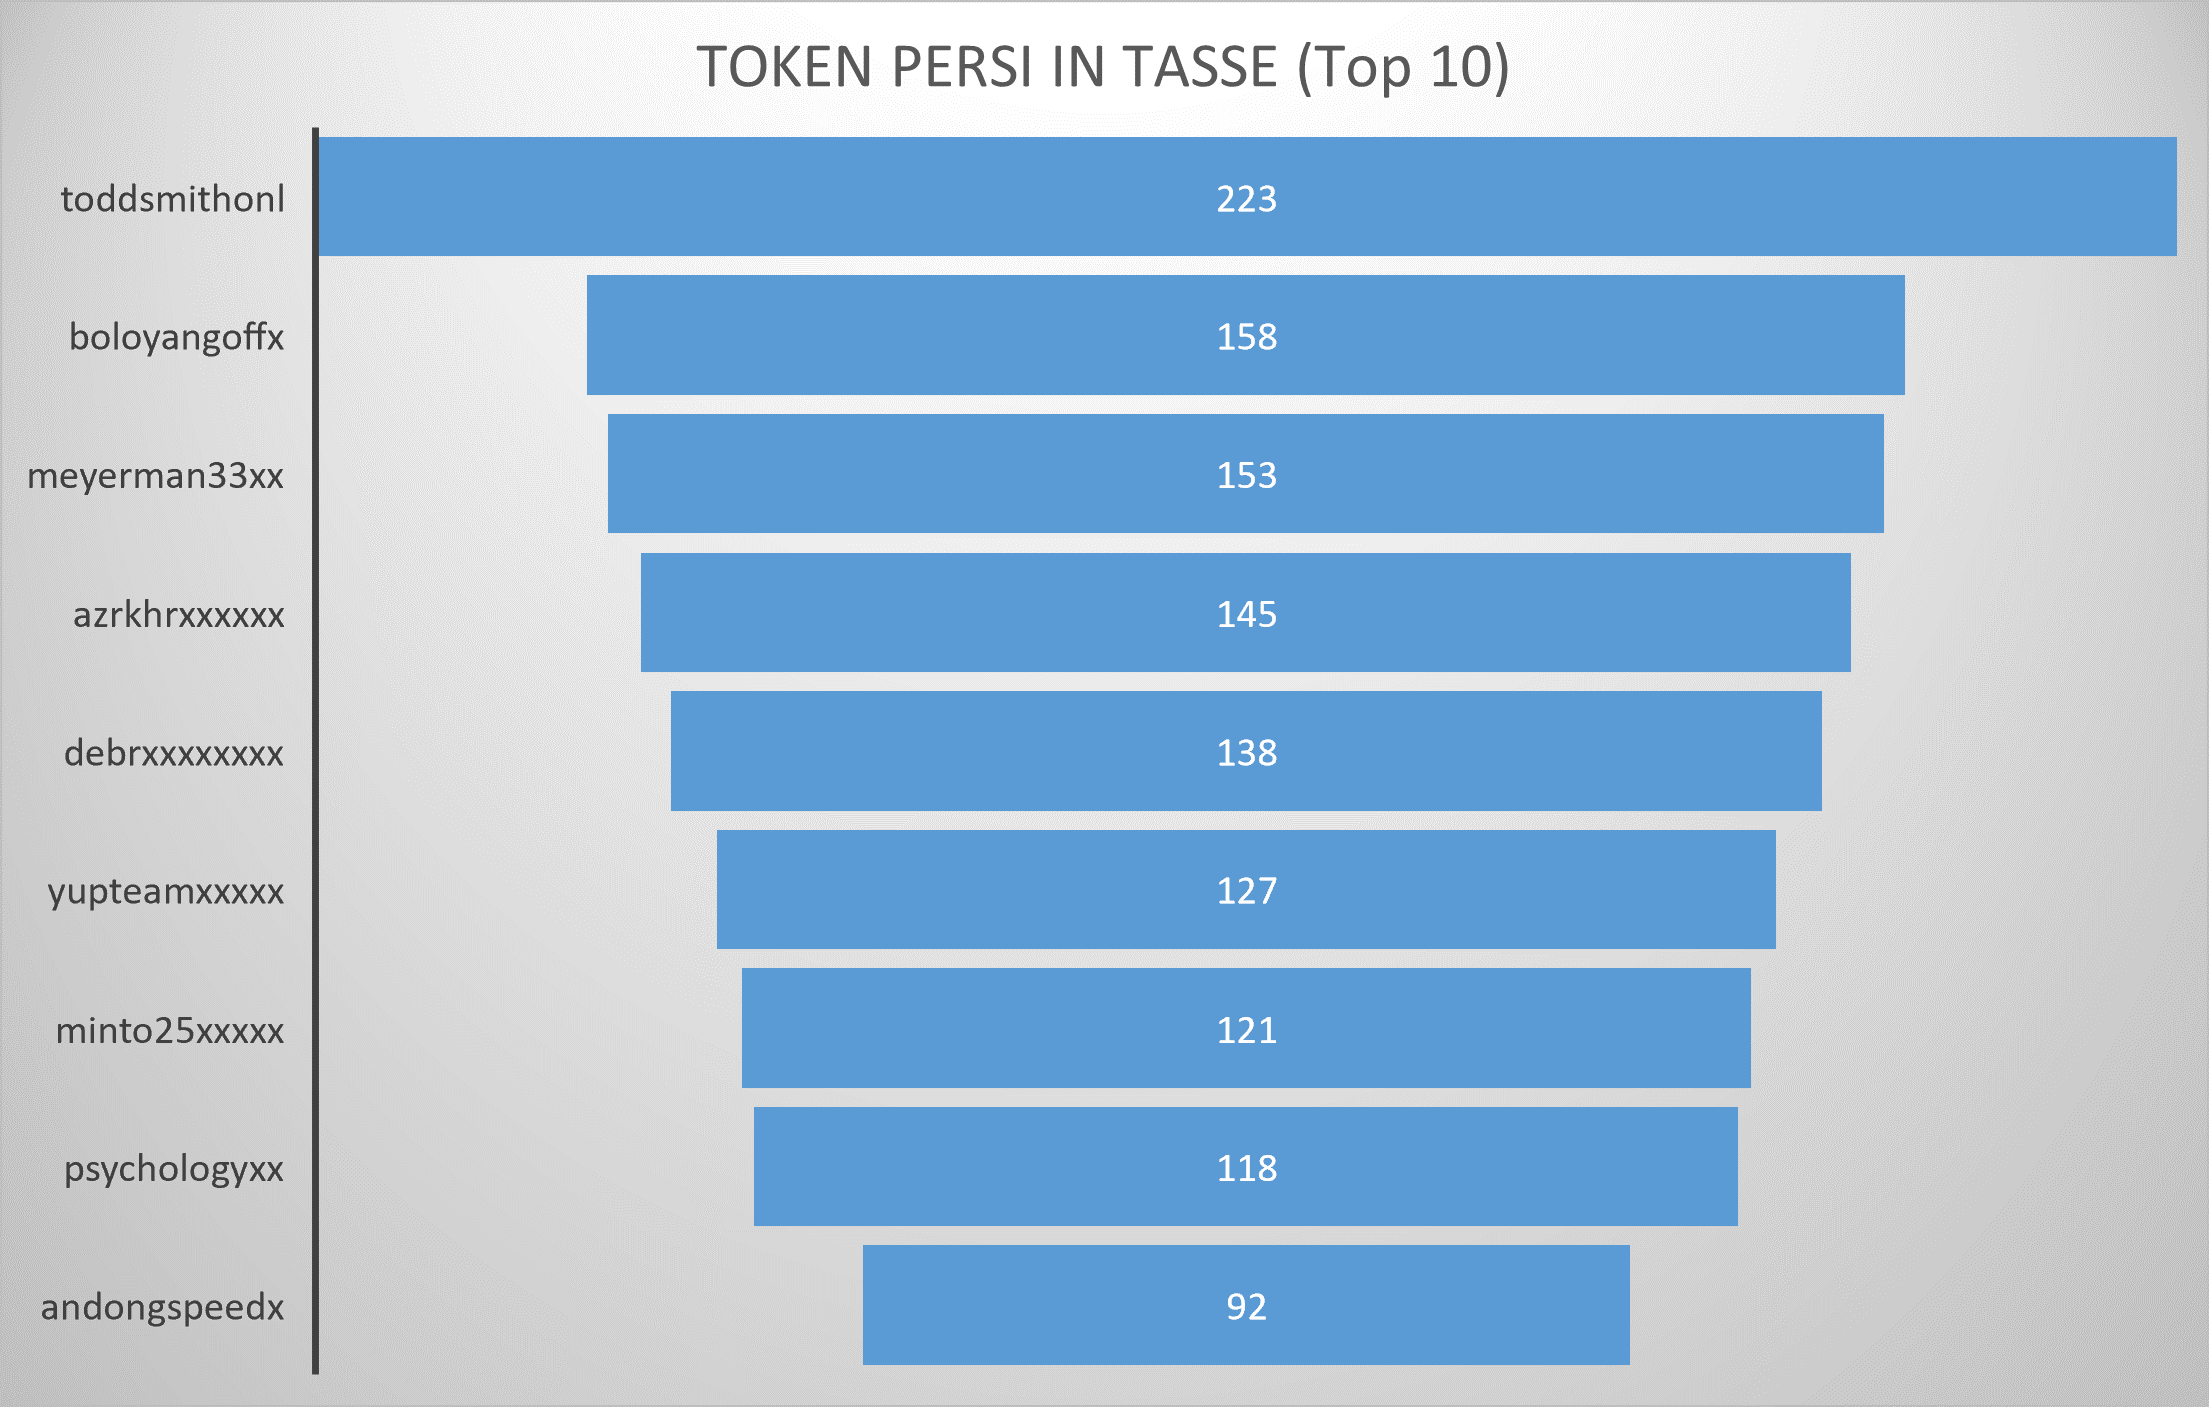
\includegraphics[width=.7\textwidth]{graphs/top10_fees.png}
    \caption{Top 10 degli account che hanno perso la maggior quantità di token in tasse}
    \label{fig: top10_fees}
\end{figure}

Notiamo come il numero dei bridge e quello dei pagamenti tasse differisca di uno. L'ipotesi è che questo sia stato effettuato in un periodo in cui la commissione fosse equivalente a 0, anche se è possibile si tratti semplicemente di un bug.

In conclusione possiamo affermare come ci sia un utilizzo del servizio del Bridge generalmente ristretto a pochi utenti, ma che è in grado di spostare ingenti somme di token.
Uno dei motivi che potrebbe ostacolare un più largo utilizzo di questo sistema è sicuramente legato al fatto che effettuare un trasferimento di token su Ethereum comporta il pagamento di una commissione. 

\section{Distribuzione Token}

\begin{figure}[t]
    \centering
    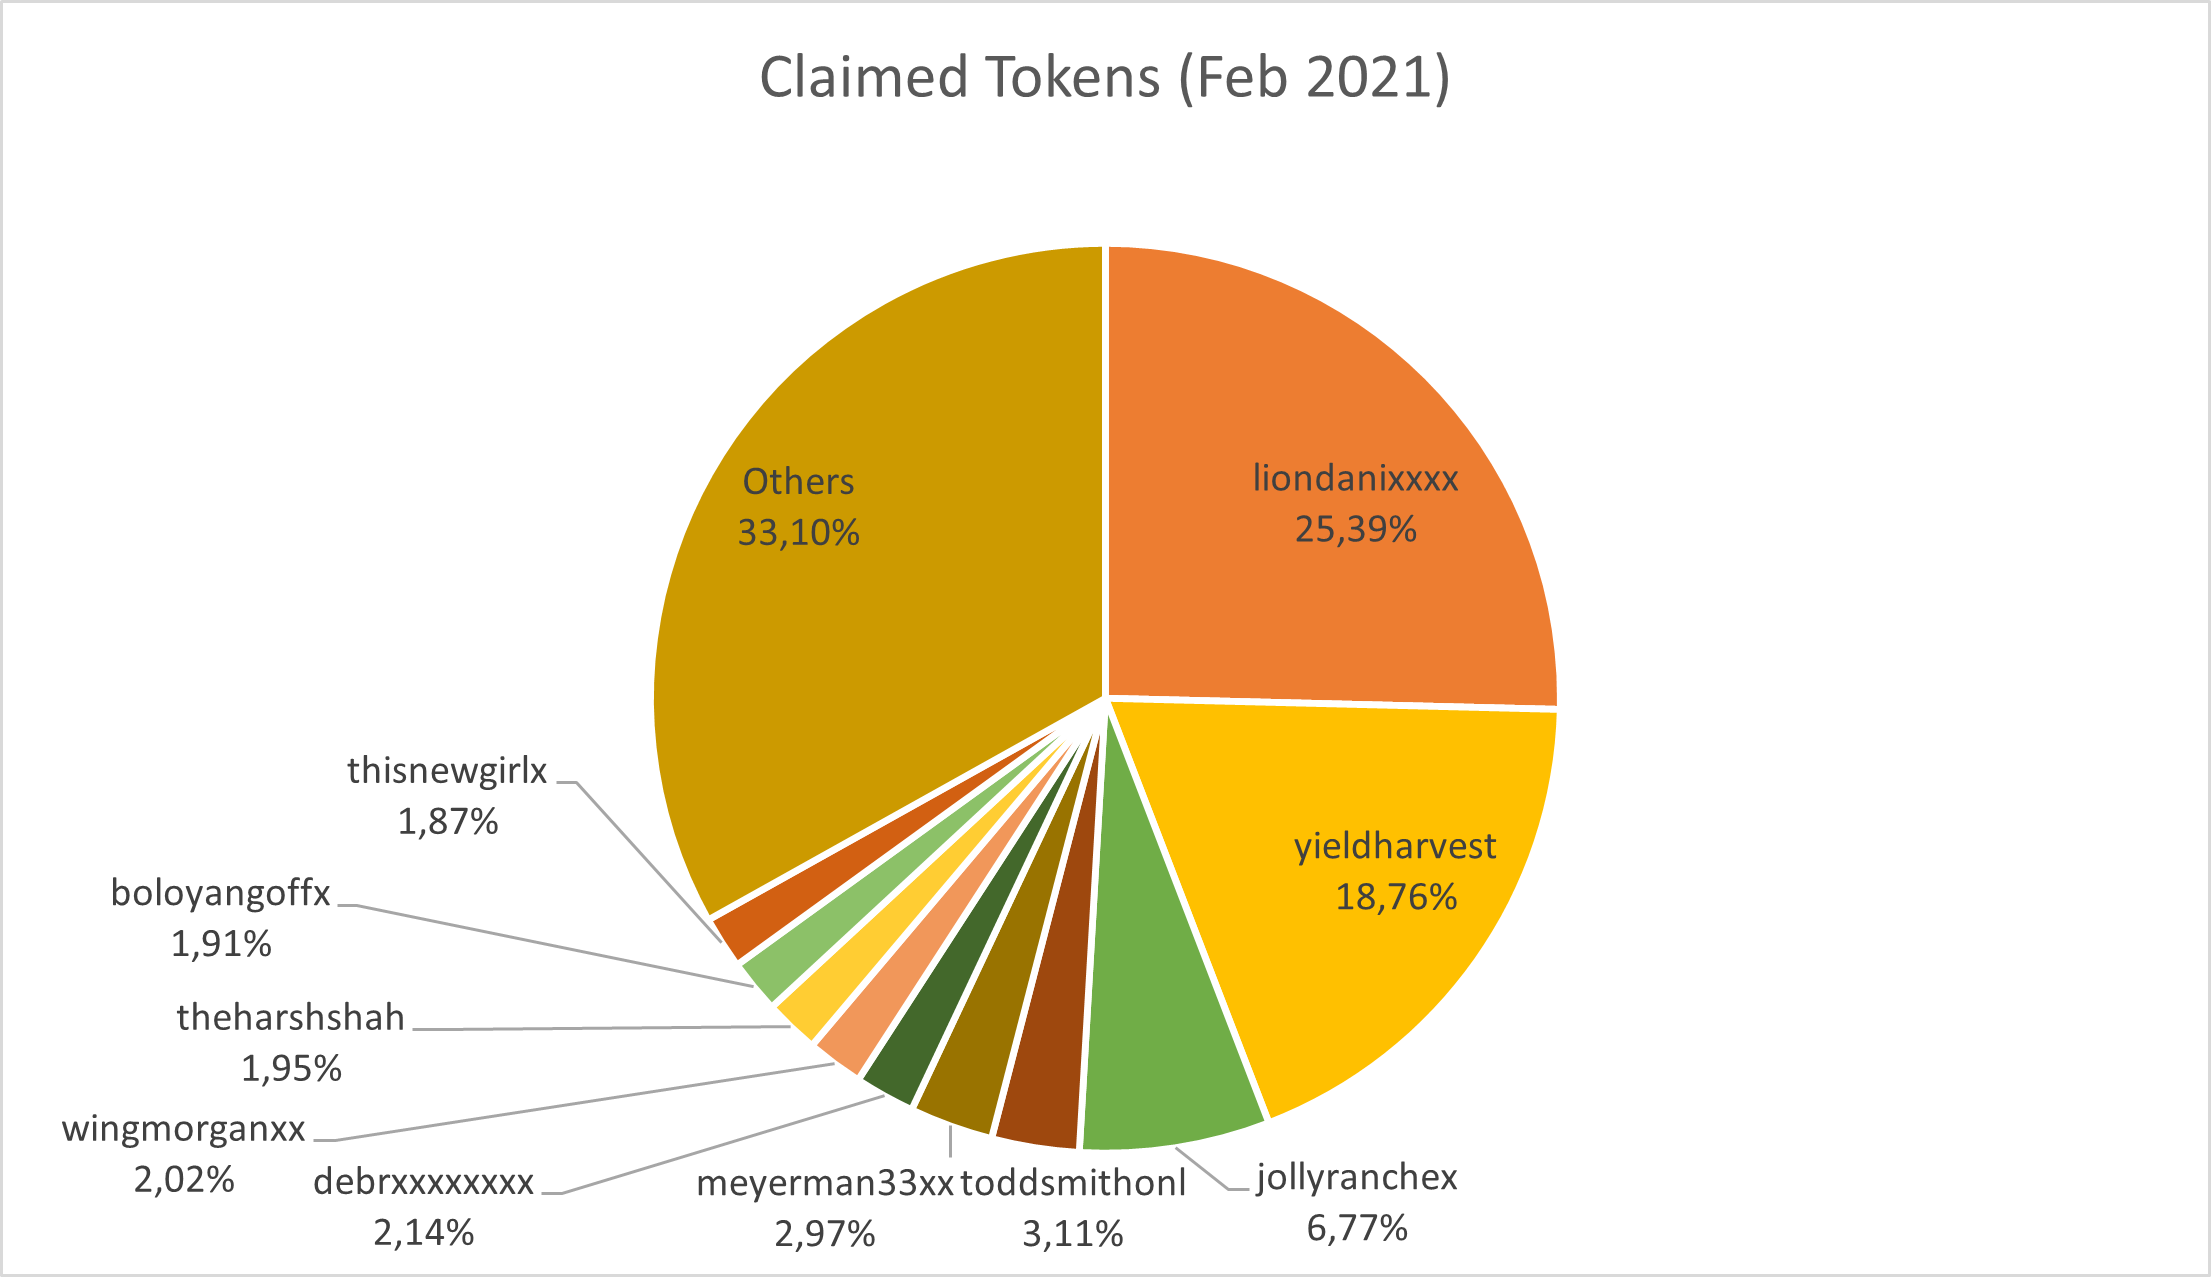
\includegraphics[width=1\textwidth]{graphs/token_claimed_february.png}
    \caption{Top 10 degli utenti che hanno guadagnato più token fino a Febbraio 2021. In \textbf{others} sono inclusi tutti gli utenti restanti.}
    \label{fig: tokens_claimed_feb}
\end{figure}    
    %\vspace*{\floatstep}
\begin{figure}[t]
    \centering
    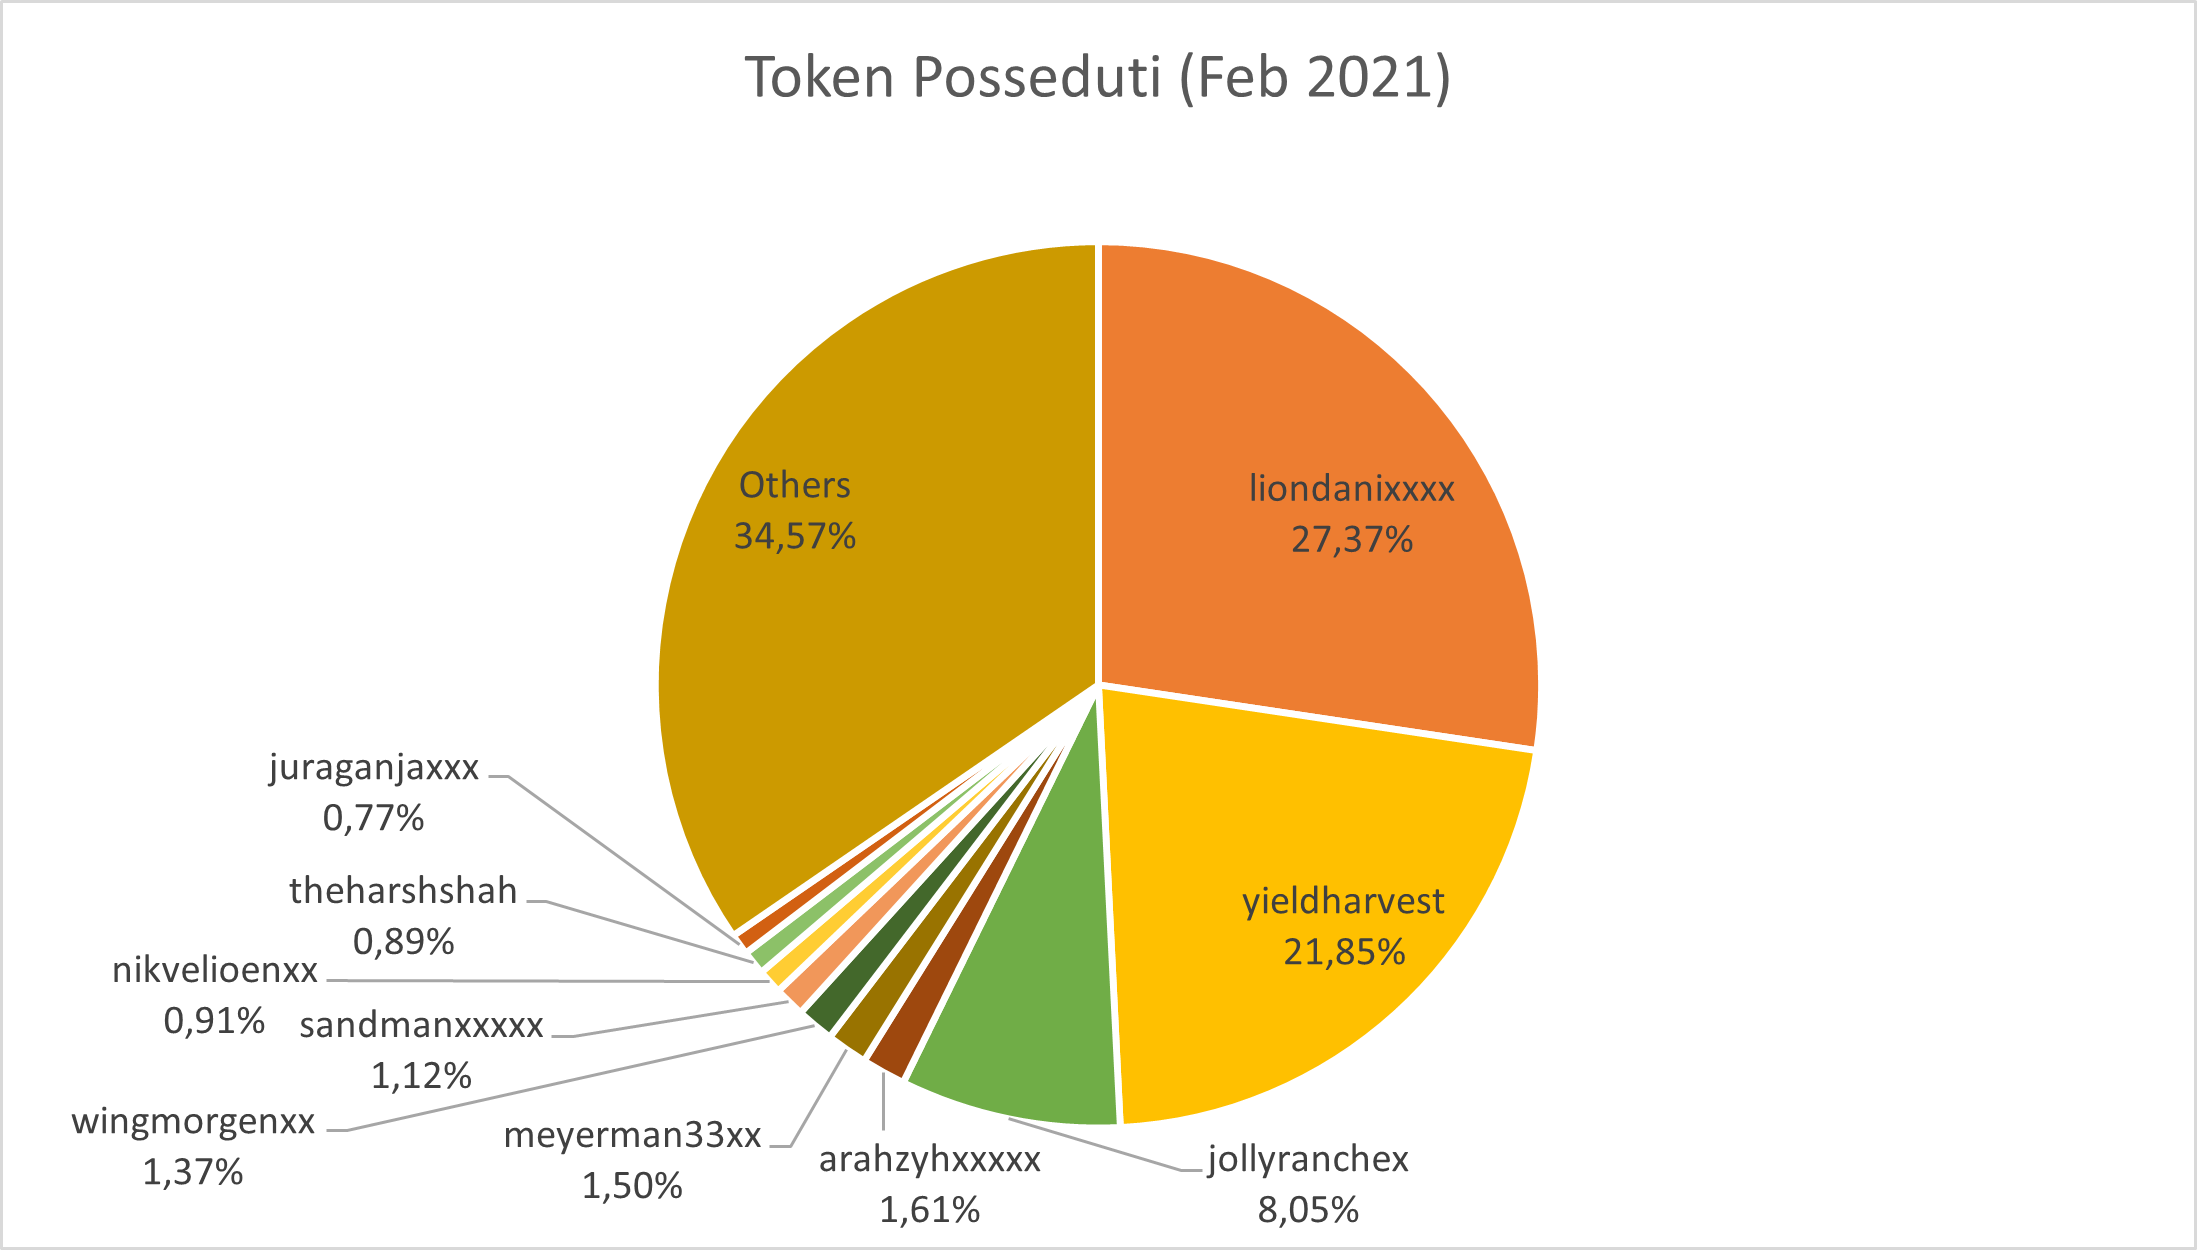
\includegraphics[width=1\textwidth]{graphs/token_posseduti_february.png}
    \caption{Top 10 degli utenti che possiedono più token a Febbraio 2021. In \textbf{others} sono inclusi tutti gli utenti restanti.}
    \label{fig: tokens_hold_feb}
\end{figure}

L'ultimo oggetto delle nostre analisi è quello dello studio in generale della distribuzione dei token tra gli utenti Yup. In particolare abbiamo deciso di concentrarci sugli account che hanno guadagnato di più e su quelli che possiedono attualmente più token.

Dopo esserci fatti un'idea dell'utilizzo di Bridge e della quantità di token migrati su Ethereum o persi in tasse, vedremo gli utenti che hanno ottenuto più ricompense e che possedevano più token nel mese di Febbraio 2021 (rispettivamente Figura \ref{fig: tokens_claimed_feb} e \ref{fig: tokens_hold_feb}) e in quello di Marzo 2021 (rispettivamente Figura \ref{fig: tokens_claimed_march} e \ref{fig: tokens_hold_march}.
Precisiamo che i token "claimed", cioè ottenuti tramite l'assegnazione delle ricompense, non indicano per forza quelli di cui l'utente è ancora in possesso poiché i token possono essere trasferiti ad altri utenti Yup, come mance sotto forma di azioni transfer, o su un suo wallet Ethereum, tramite il Bridge.


\begin{figure}[t]
    \centering
    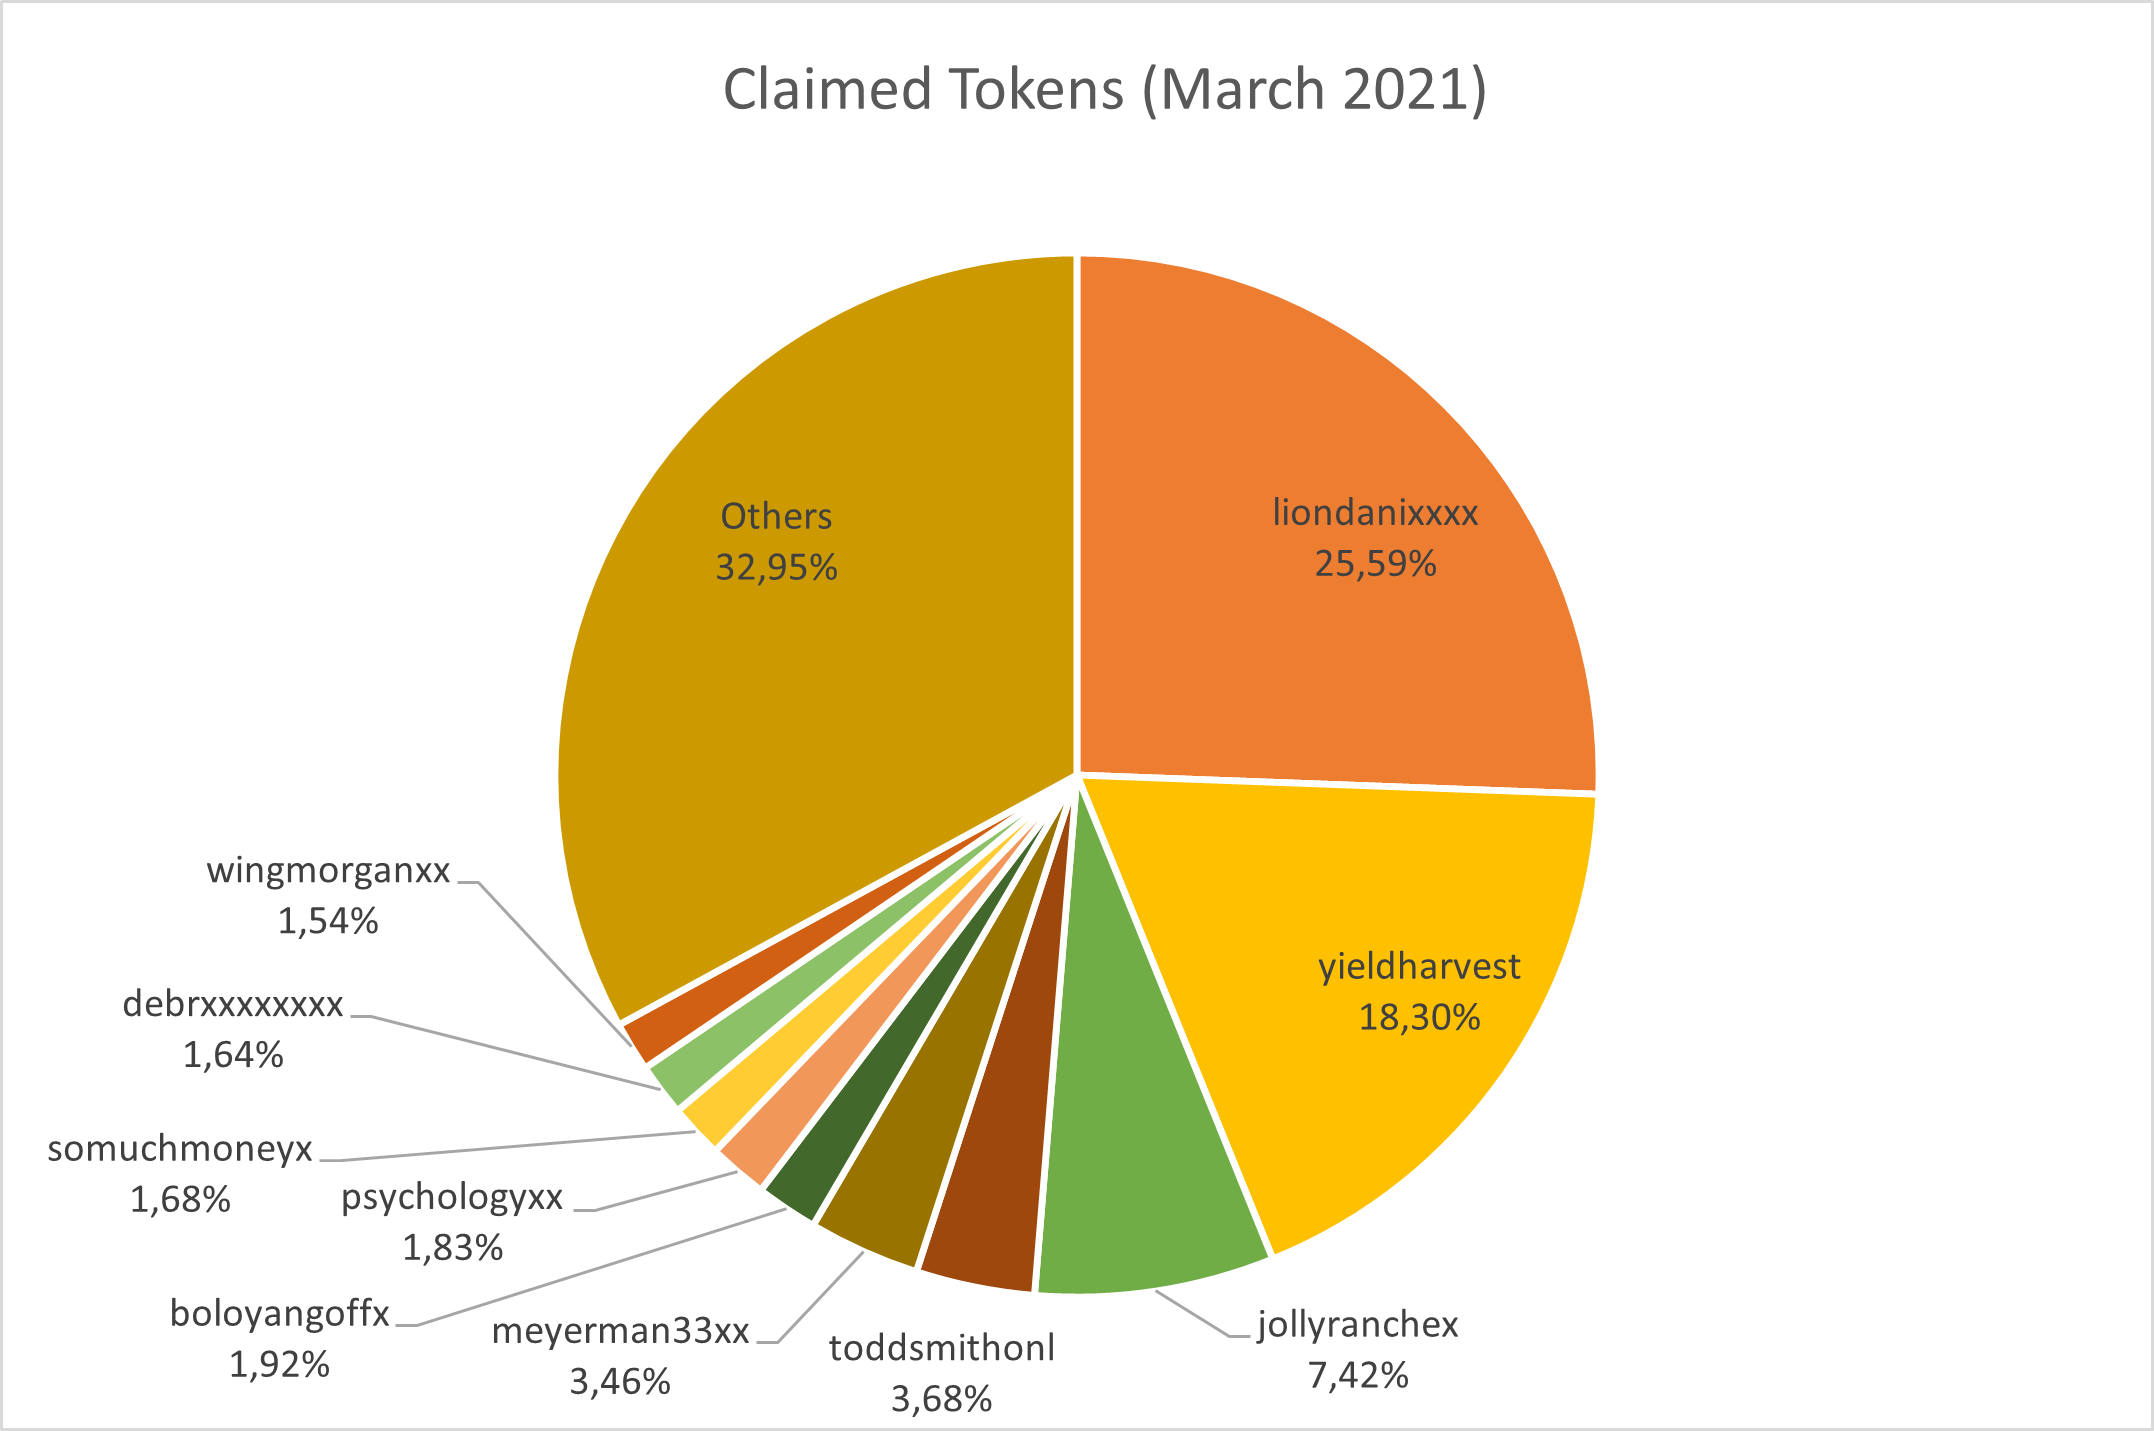
\includegraphics[width=1\textwidth]{graphs/token_claimed_march.png}
    \caption{Top 10 degli utenti che hanno guadagnato più token fino a Marzo 2021. In \textbf{others} sono inclusi tutti gli utenti restanti.}
    \label{fig: tokens_claimed_march}
\end{figure}    
    %\vspace*{\floatstep}
\begin{figure}[t]
    \centering
    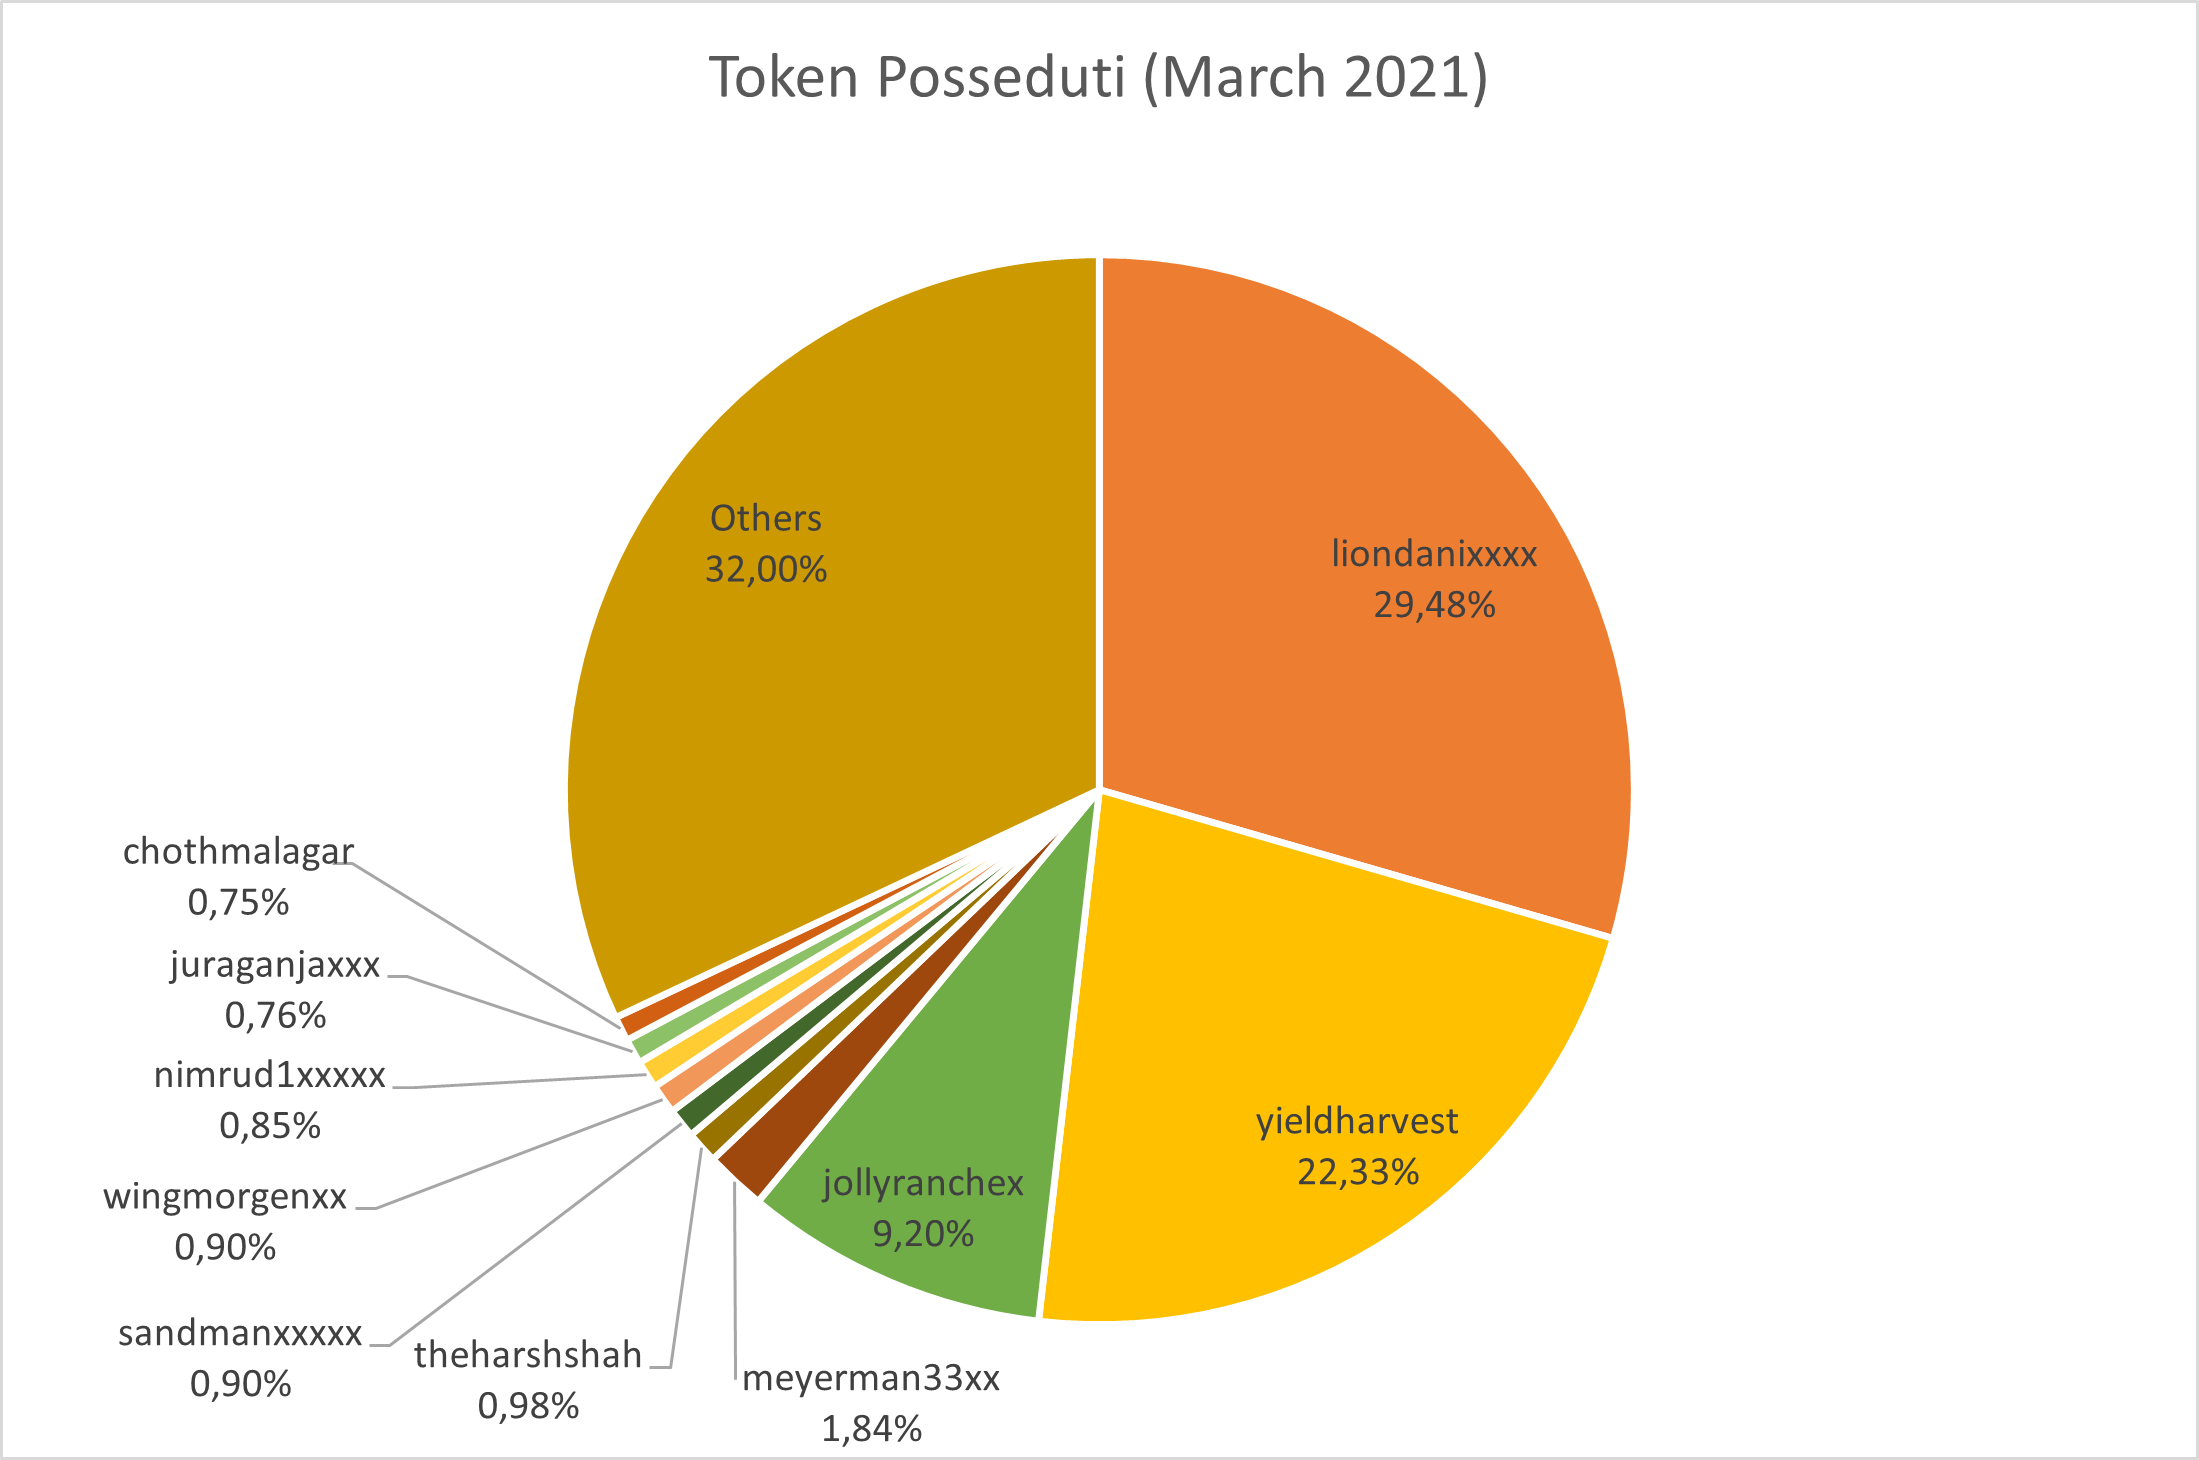
\includegraphics[width=1\textwidth]{graphs/token_posseduti_march.png}
    \caption{Top 10 degli utenti che possiedono più token a Marzo 2021. In \textbf{others} sono inclusi tutti gli utenti restanti.}
    \label{fig: tokens_hold_march}
\end{figure}

%\todo[inline]{non ho capito la differenza tra le due figure. le prime due sono tutti i dati fino a febbraio e le seconde due sono tutti i dati fino a Marzo? [EDITED: si]}

Da notare come le classifiche dei token posseduti o riscossi, indipendentemente dal fatto che si consideri il mese di Febbraio o Marzo 2021, siano dominate da utenti che, oltre ad utilizzare la piattaforma, forniscono liquidità al protocollo: \textit{liondanixxxx}, \textit{yieldharvest}, \textit{jollyranchex}, \textit{toddsmithonl}, \textit{meyerman33xx}. Questi ultimi, oltre che a detenere le prime posizioni in classifica, possiedono sostanzialmente gran parte dei token in circolazione all'interno della community, ovvero più del 57\% nel mese di Febbraio (Figura \ref{fig: tokens_hold_feb} e più del 61\% nel mese di Marzo (Figura \ref{fig: tokens_hold_march}.

Risulta rilevante anche notare che i 3 account con più claimed tokens posseggono, in percentuale, più token di quelli claimed.
Questo importante fatto ci mostra che dietro le attività di voto esiste una certa economia di scambio di monete e che alcuni utenti riescono ad arricchirsi non necessariamente solo tramite il meccanismo del voto.
Infine, confrontando i risultati ottenuti a Febbraio 2021 con quelli ottenuti a Marzo 2021, risulta chiaro, non solo che la maggior parte della ricchezza della piattaforma è gestita da un numero esiguo di utenti (i 3 utenti più ricchi gestiscono più di metà del patrimonio in circolazione), ma anche che questi 3 utenti si stiano arricchendo di più nel tempo e che quindi il divario tra i più ricchi e tutto il resto degli utenti si stia acutizzando.

\section{Analisi Giornaliera}
Come ultima analisi ci siamo concentrati su uno studio approfondito delle azioni registrate nei mesi di Agosto e Settembre 2020, non più su base mensile, ma bensì giornaliera. L'analisi è stata effettuata con lo scopo di individuare attività inusuale in determinati giorni di quei mesi in cui era stata riscontrata maggiore attività.


In Figura \ref{fig: actions_daily} possiamo osservare la distribuzione giornaliera di tutte le azioni registrate nei mesi in oggetto della nostra analisi.

\begin{figure}[t]
    \centering
    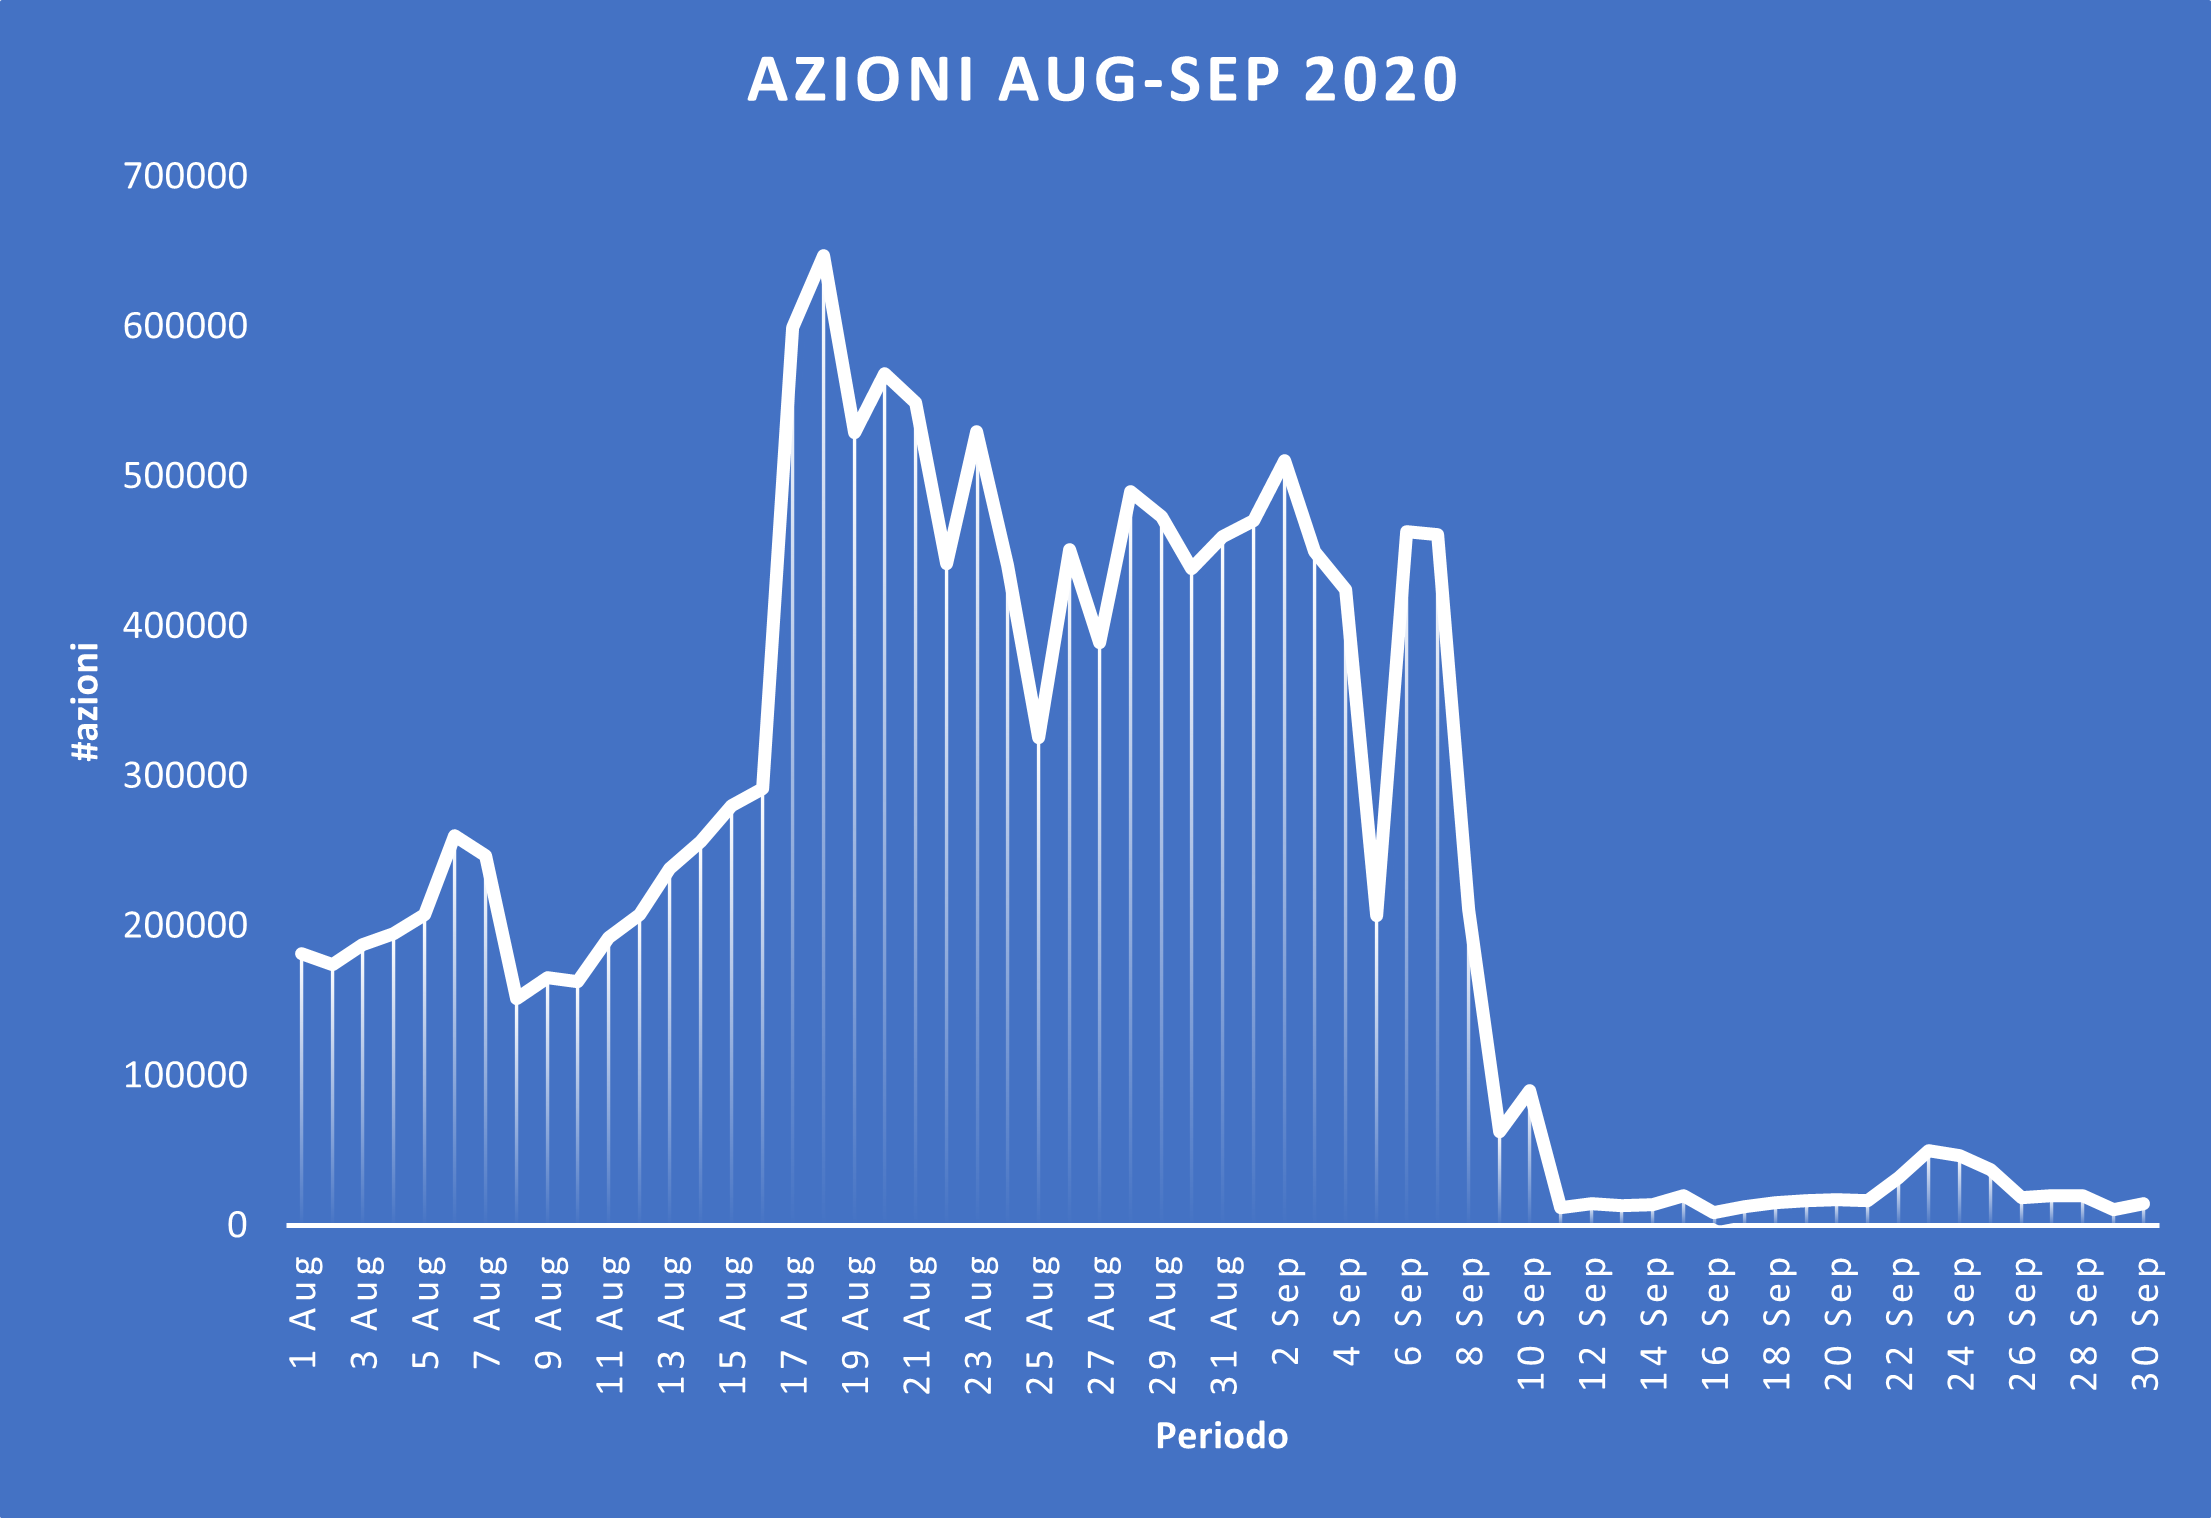
\includegraphics[width=0.8\textwidth]{graphs/daily_azioni.png}
    \caption{Distribuzione giornaliera di tutte le azioni, account Mirror inclusi.}
    \label{fig: actions_daily}
\end{figure}

La Figura ci mostra un'attività sostenuta, con circa 200.000 azioni al giorno fin dall'inizio del mese di Agosto.
L'attività su Yup si intensifica ulteriormente intorno alla metà del mese, superando le 400.000 azioni al giorno, ad eccezione di rari casi.
L'attività rimane molto alta fino all'inizio di Settembre, momento nel quale subisce un brusco arresto, fino quasi a sparire fino alla fine del mese.
Le cause di questo fenomeno non sono chiare, anche se possiamo ipotizzare che sono dovute a problemi tecnici legati alla blockchain EOS.
Infatti, come spiegato nel Capitolo \ref{chapter_background}, per poter effettuare azioni su EOS è necessario pagare un costo non trascurabile, in particolare di RAM e CPU.
Potrebbe essere accaduto che, in concomitanza con la nuova massa di utenti iscritta alla piattaforma, e l'algoritmo utilizzato per determinare la ricompensa, lo smart contract che gestisce la piattaforma non sia più stato in grado di calcolare le ricompense o di accettare voti.
Questi problemi tecnici potrebbero aver portato gli sviluppatori ad aver disabilitato alcuni account Mirror, come anche mostrato in Figura \ref{fig:attivi_conmirr}.

In Figura \ref{fig: createacct_daily_conmirr} e \ref{fig: createacct_daily_nomirr} riportiamo invece la distribuzione relativa alla creazione di account, rispettivamente considerando o meno account Mirror.

\begin{figure}[t]
    \centering
    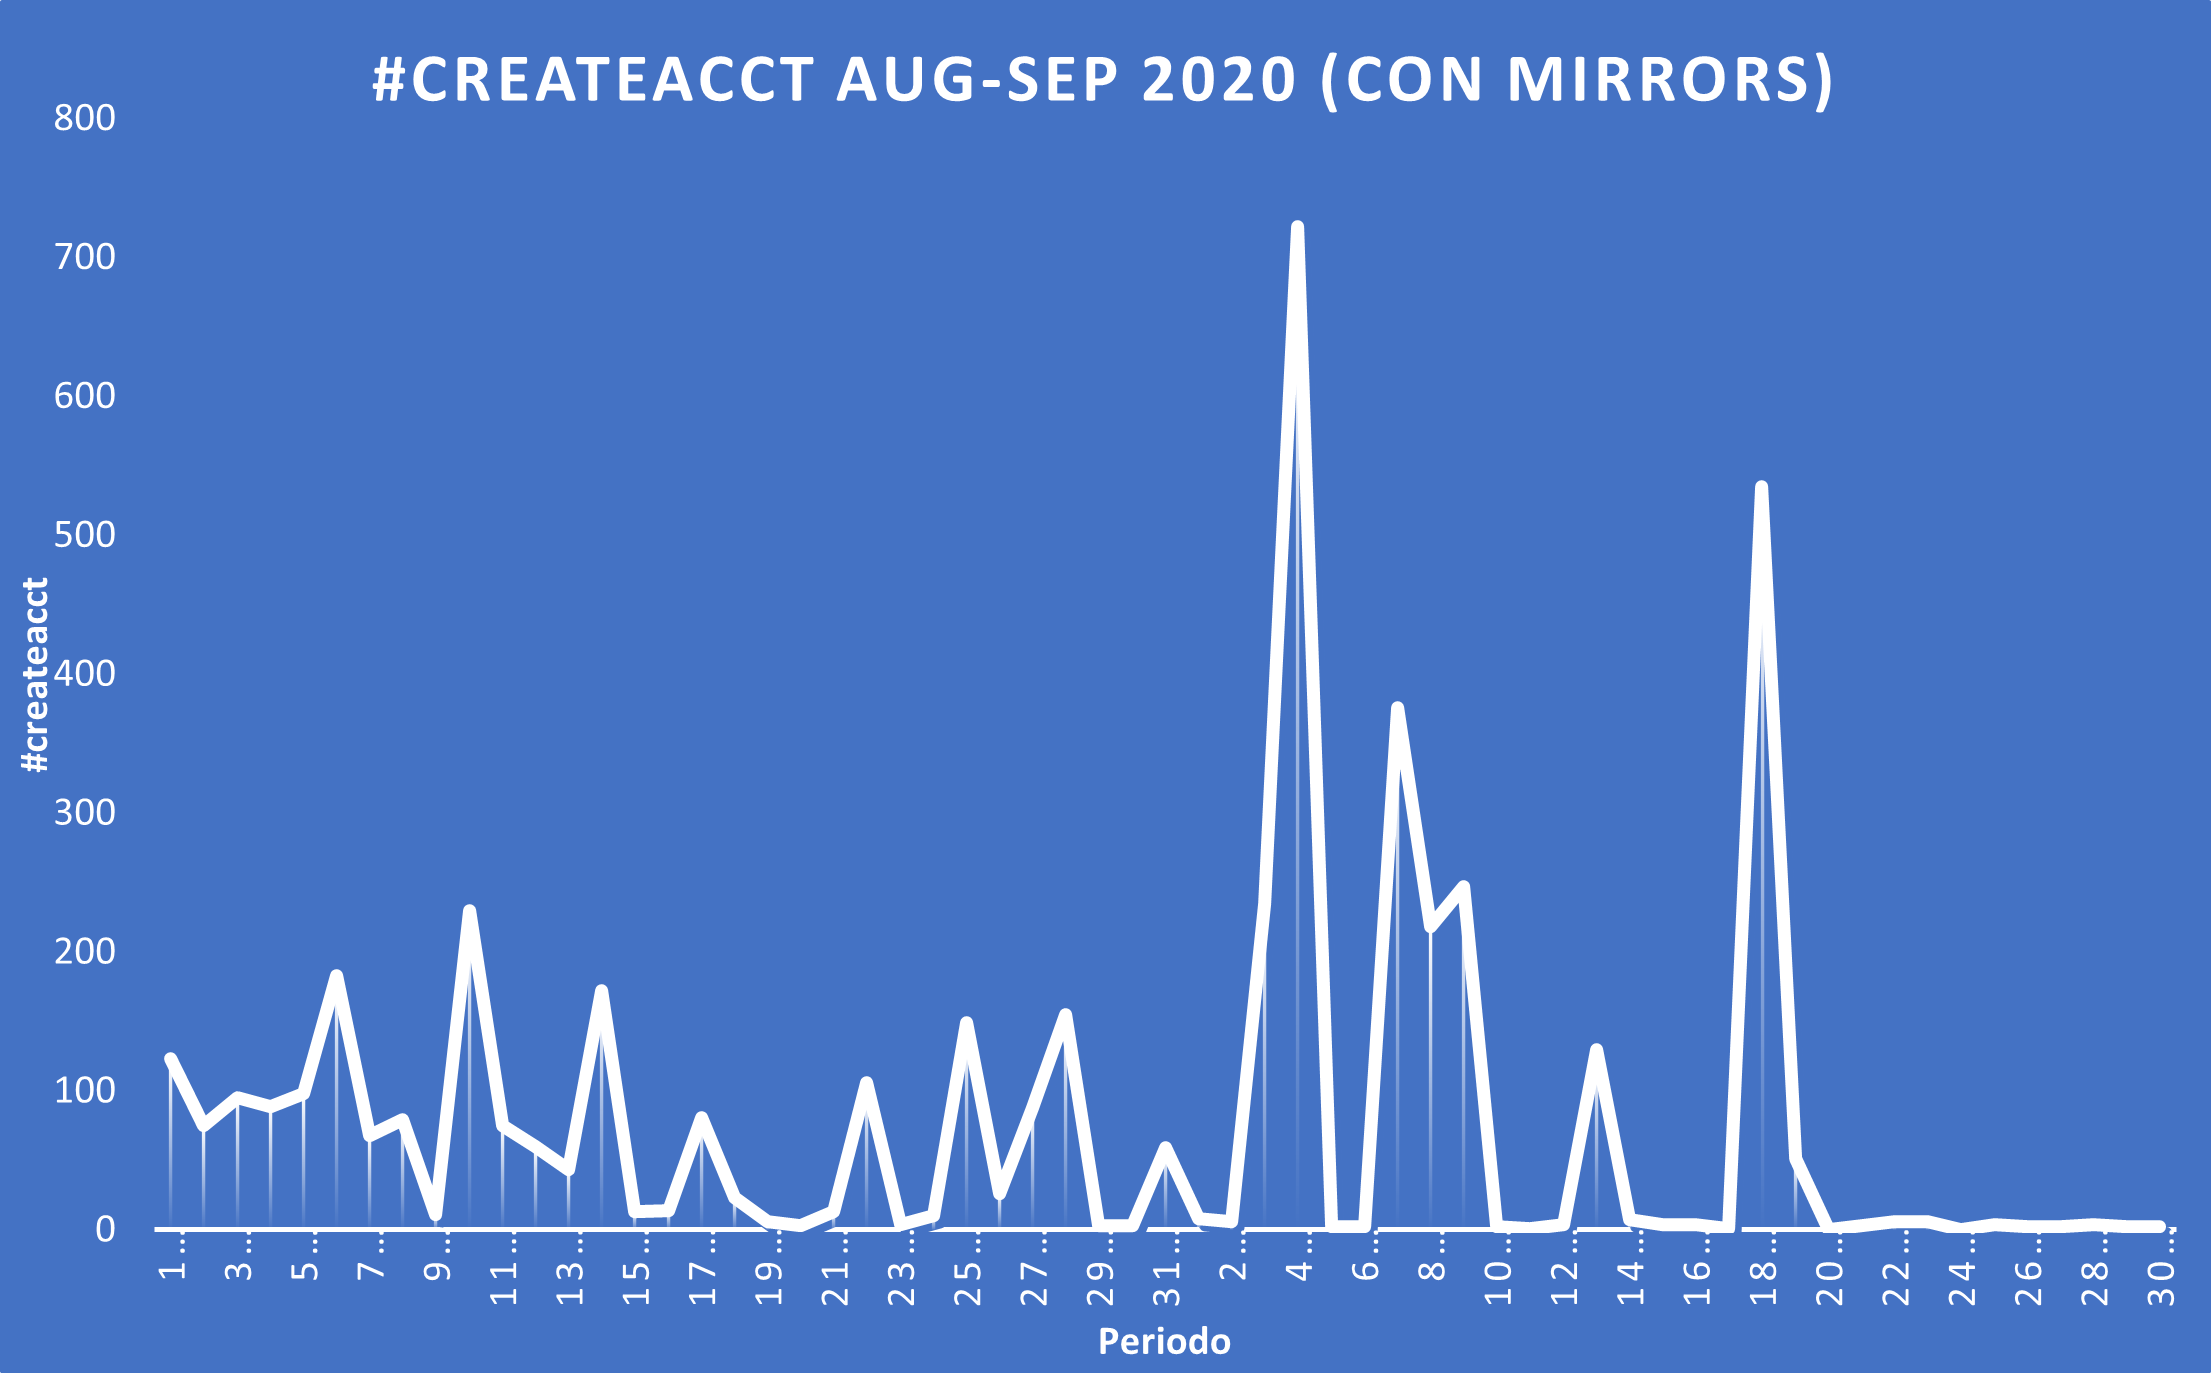
\includegraphics[width=0.8\textwidth]{graphs/daily_createacct.png}
    \caption{Distribuzione delle \textbf{createacct} su base giornaliera includendo account Mirror}
    \label{fig: createacct_daily_conmirr}
\end{figure}    
    %\vspace*{\floatstep}
\begin{figure}[t]
    \centering
    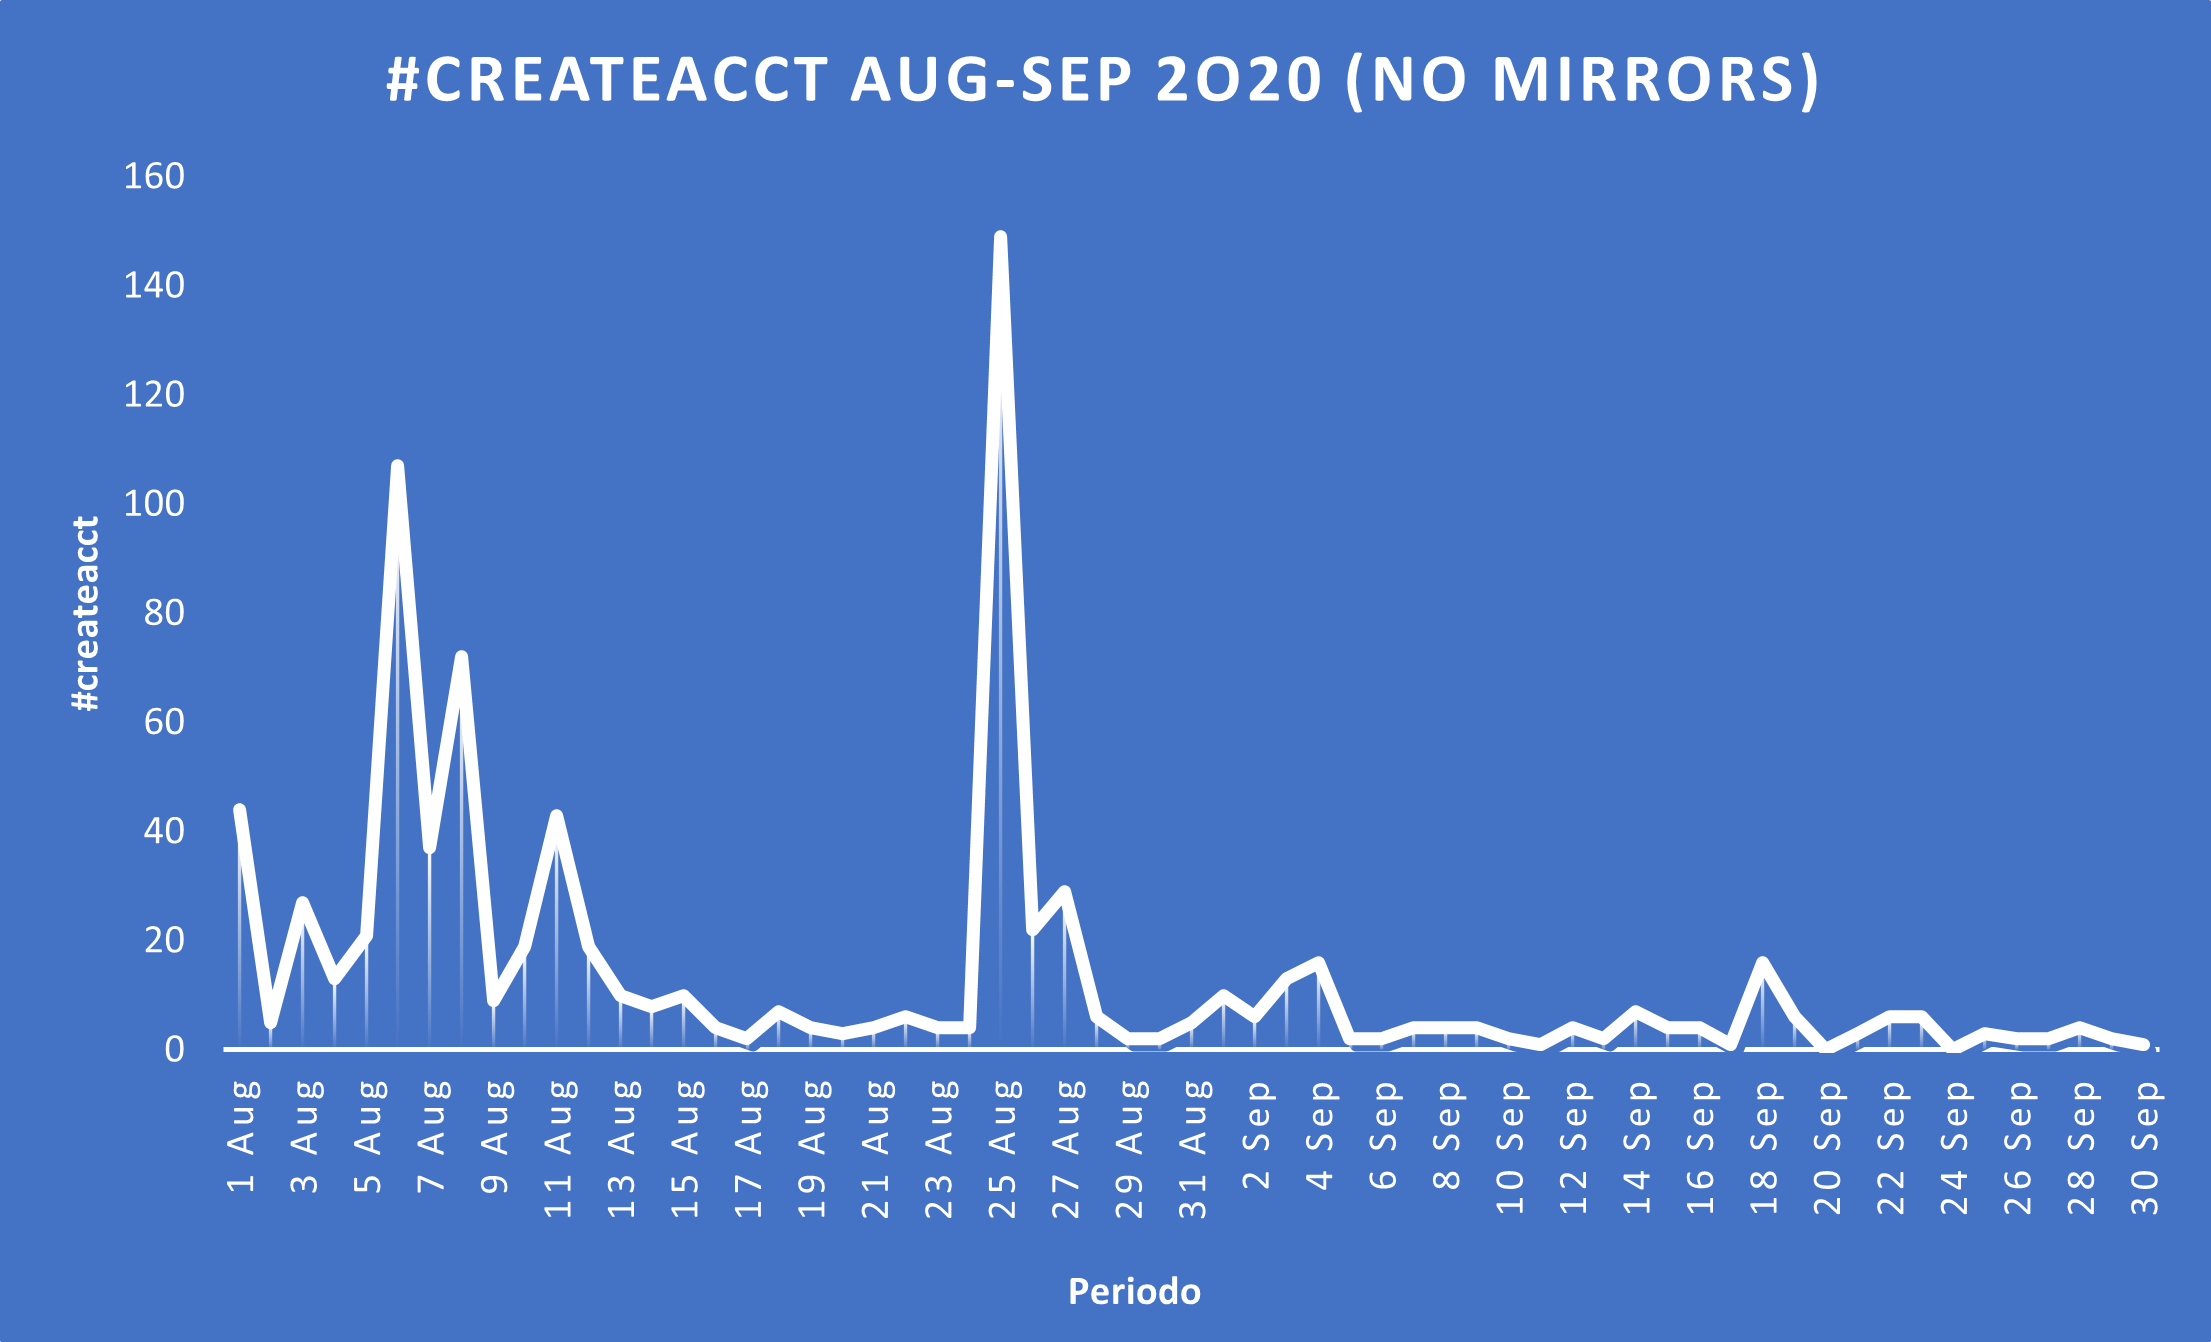
\includegraphics[width=0.8\textwidth]{graphs/daily_createacct_nomirr.png}
    \caption{Distribuzione delle \textbf{createacct} su base giornaliera escludendo account Mirror}
    \label{fig: createacct_daily_nomirr}
\end{figure}

Le Figure mostrano un andamento altalenante per quanto riguarda il numero di nuovi iscritti giornalmente.
Possiamo però notare un picco di quasi 700 nuovi account Mirror iscritti il giorno 4 Settembre e quasi 500 il giorno 18 Settembre, pochi giorni prima dei problemi tecnici ipotizzati in questa Sezione.
Siamo sicuri che siano quasi tutti Mirror perché non osserviamo picchi simili in Figura \ref{fig: createacct_daily_nomirr}.
Notiamo invece un picco di oltre 140 utenti non-Mirror iscritti il giorno 25 Agosto.

Infine i grafici su base giornaliera delle azioni di voto, Figura \ref{fig: voting_daily_conmirr} considerando tutti gli utenti, e \ref{fig: voting_daily_nomirr} senza considerare i Mirror, e degli utenti attivi, Figura \ref{fig: attivi_daily_conmirr} considerando tutti gli utenti, e \ref{fig: attivi_daily_nomirr} senza considerare i Mirror.
Abbiamo tentato di individuare qualcosa che motivasse questo picco andando a vedere se ci fossero tweet in quei giorni e in quelli antecedenti sul profilo Twitter di Yup e su quello degli influencer maggiormente votati dagli utenti (Elon Musk, Binance, ecc.), purtroppo senza successo. Il motivo di un picco del genere in quel periodo è pertanto sconosciuto.

\begin{figure}[t]
    \centering
    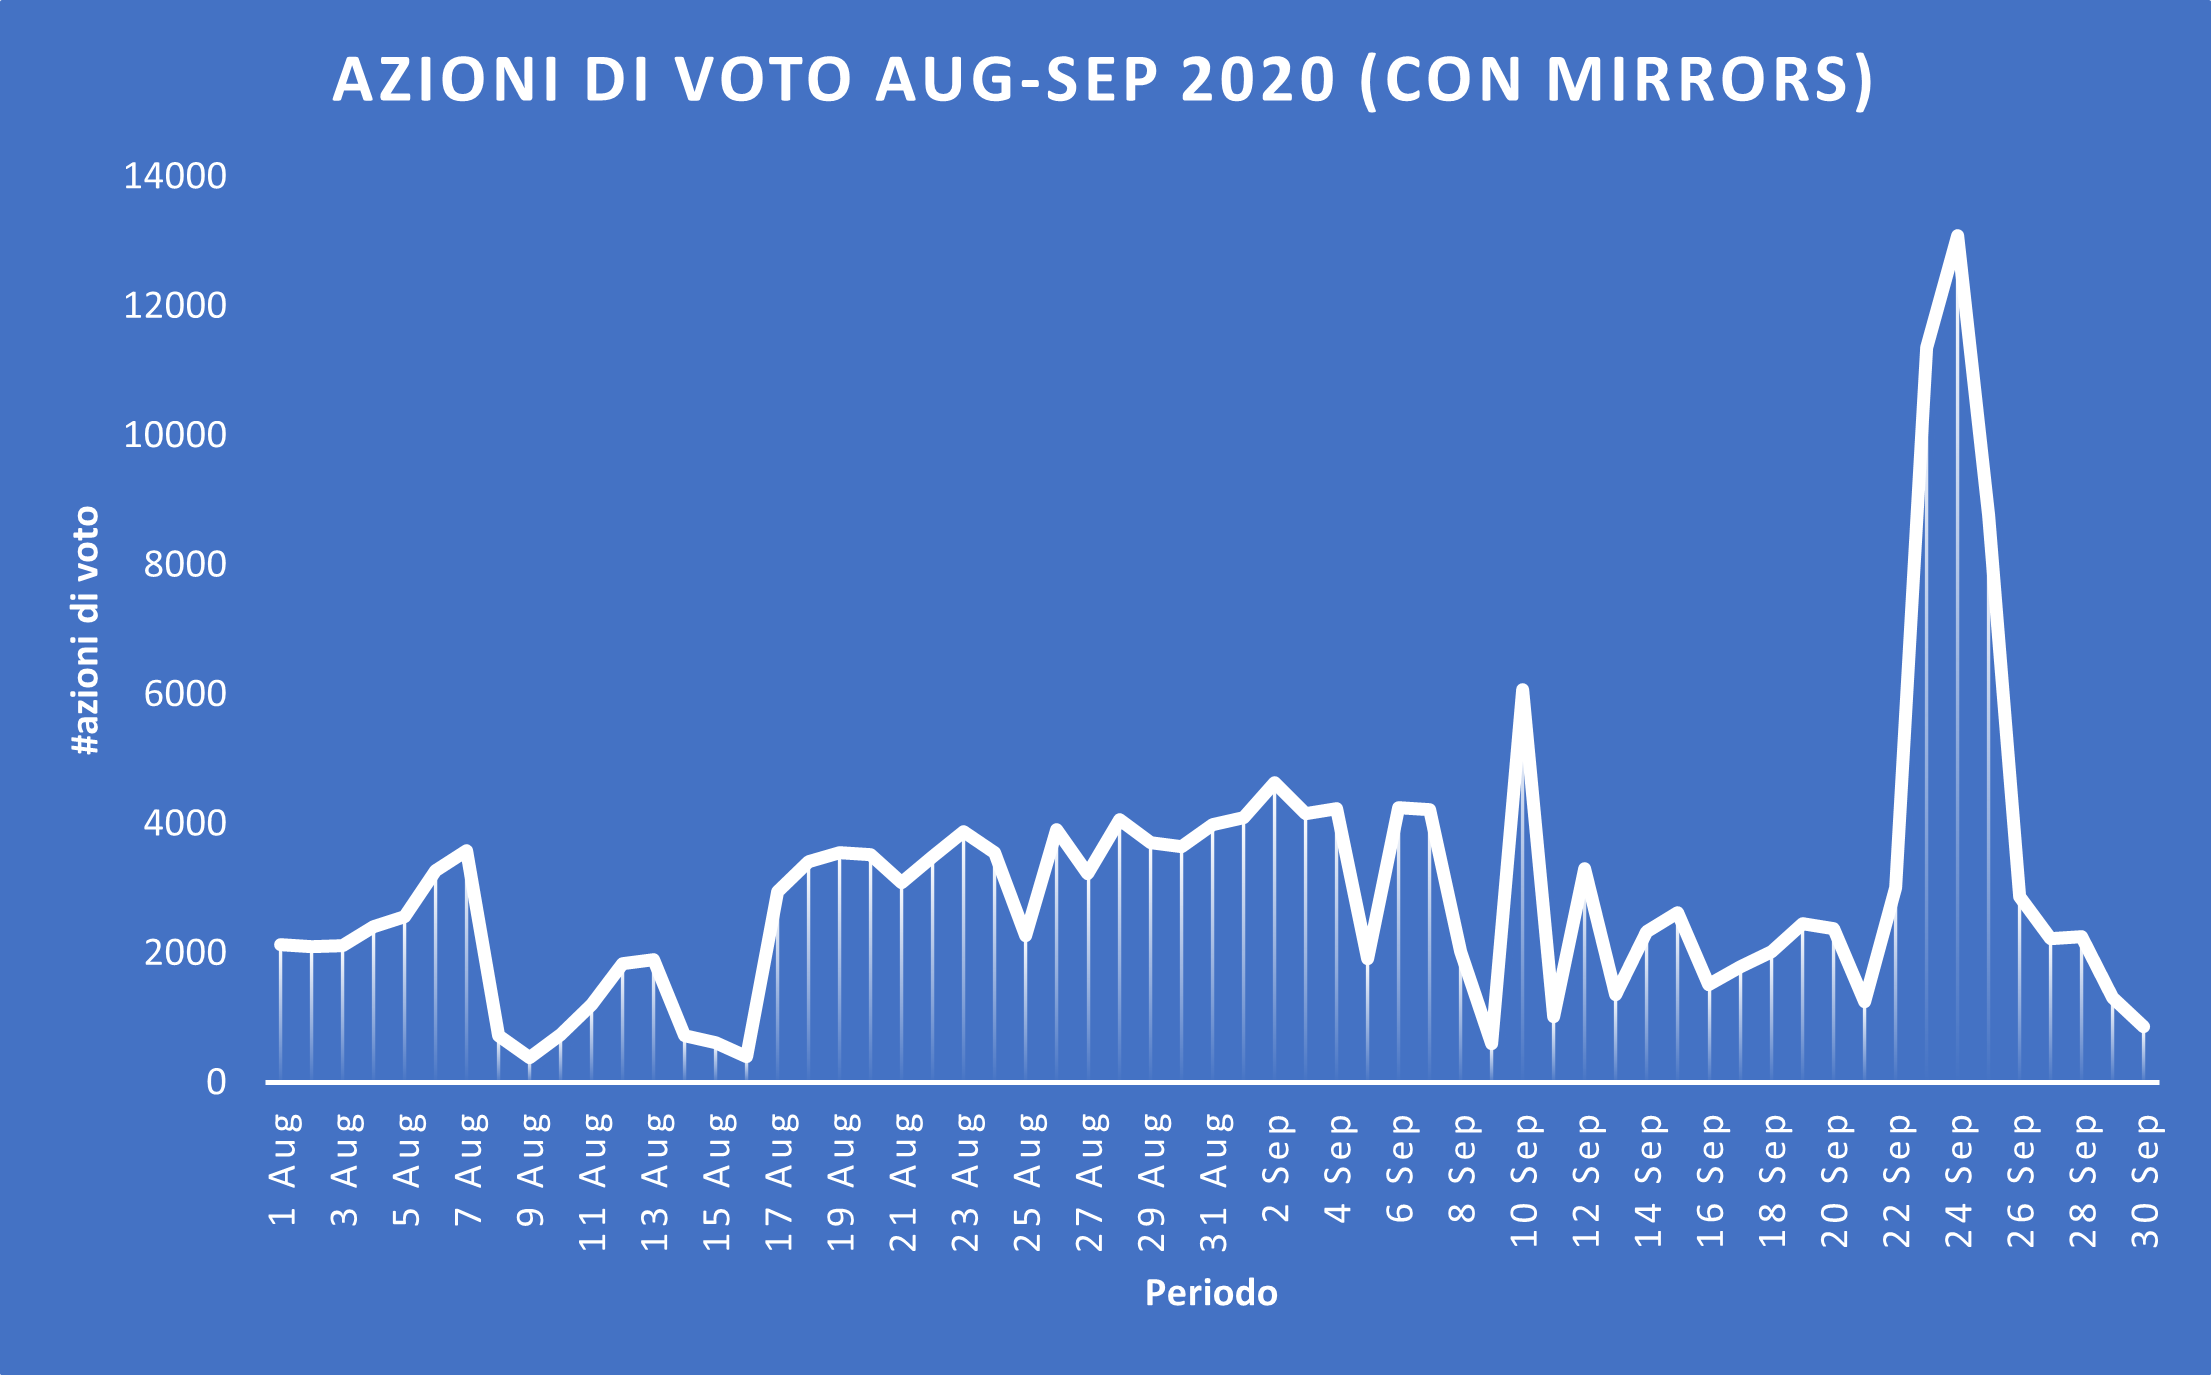
\includegraphics[width=.7\textwidth]{graphs/daily_azionivoto.png}
    \caption{Distribuzione giornaliera delle azioni di voto, incluse quelle effettuate da account mirror}
    \label{fig: voting_daily_conmirr}
\end{figure}    
    
    
\begin{figure}[t]
    \centering
    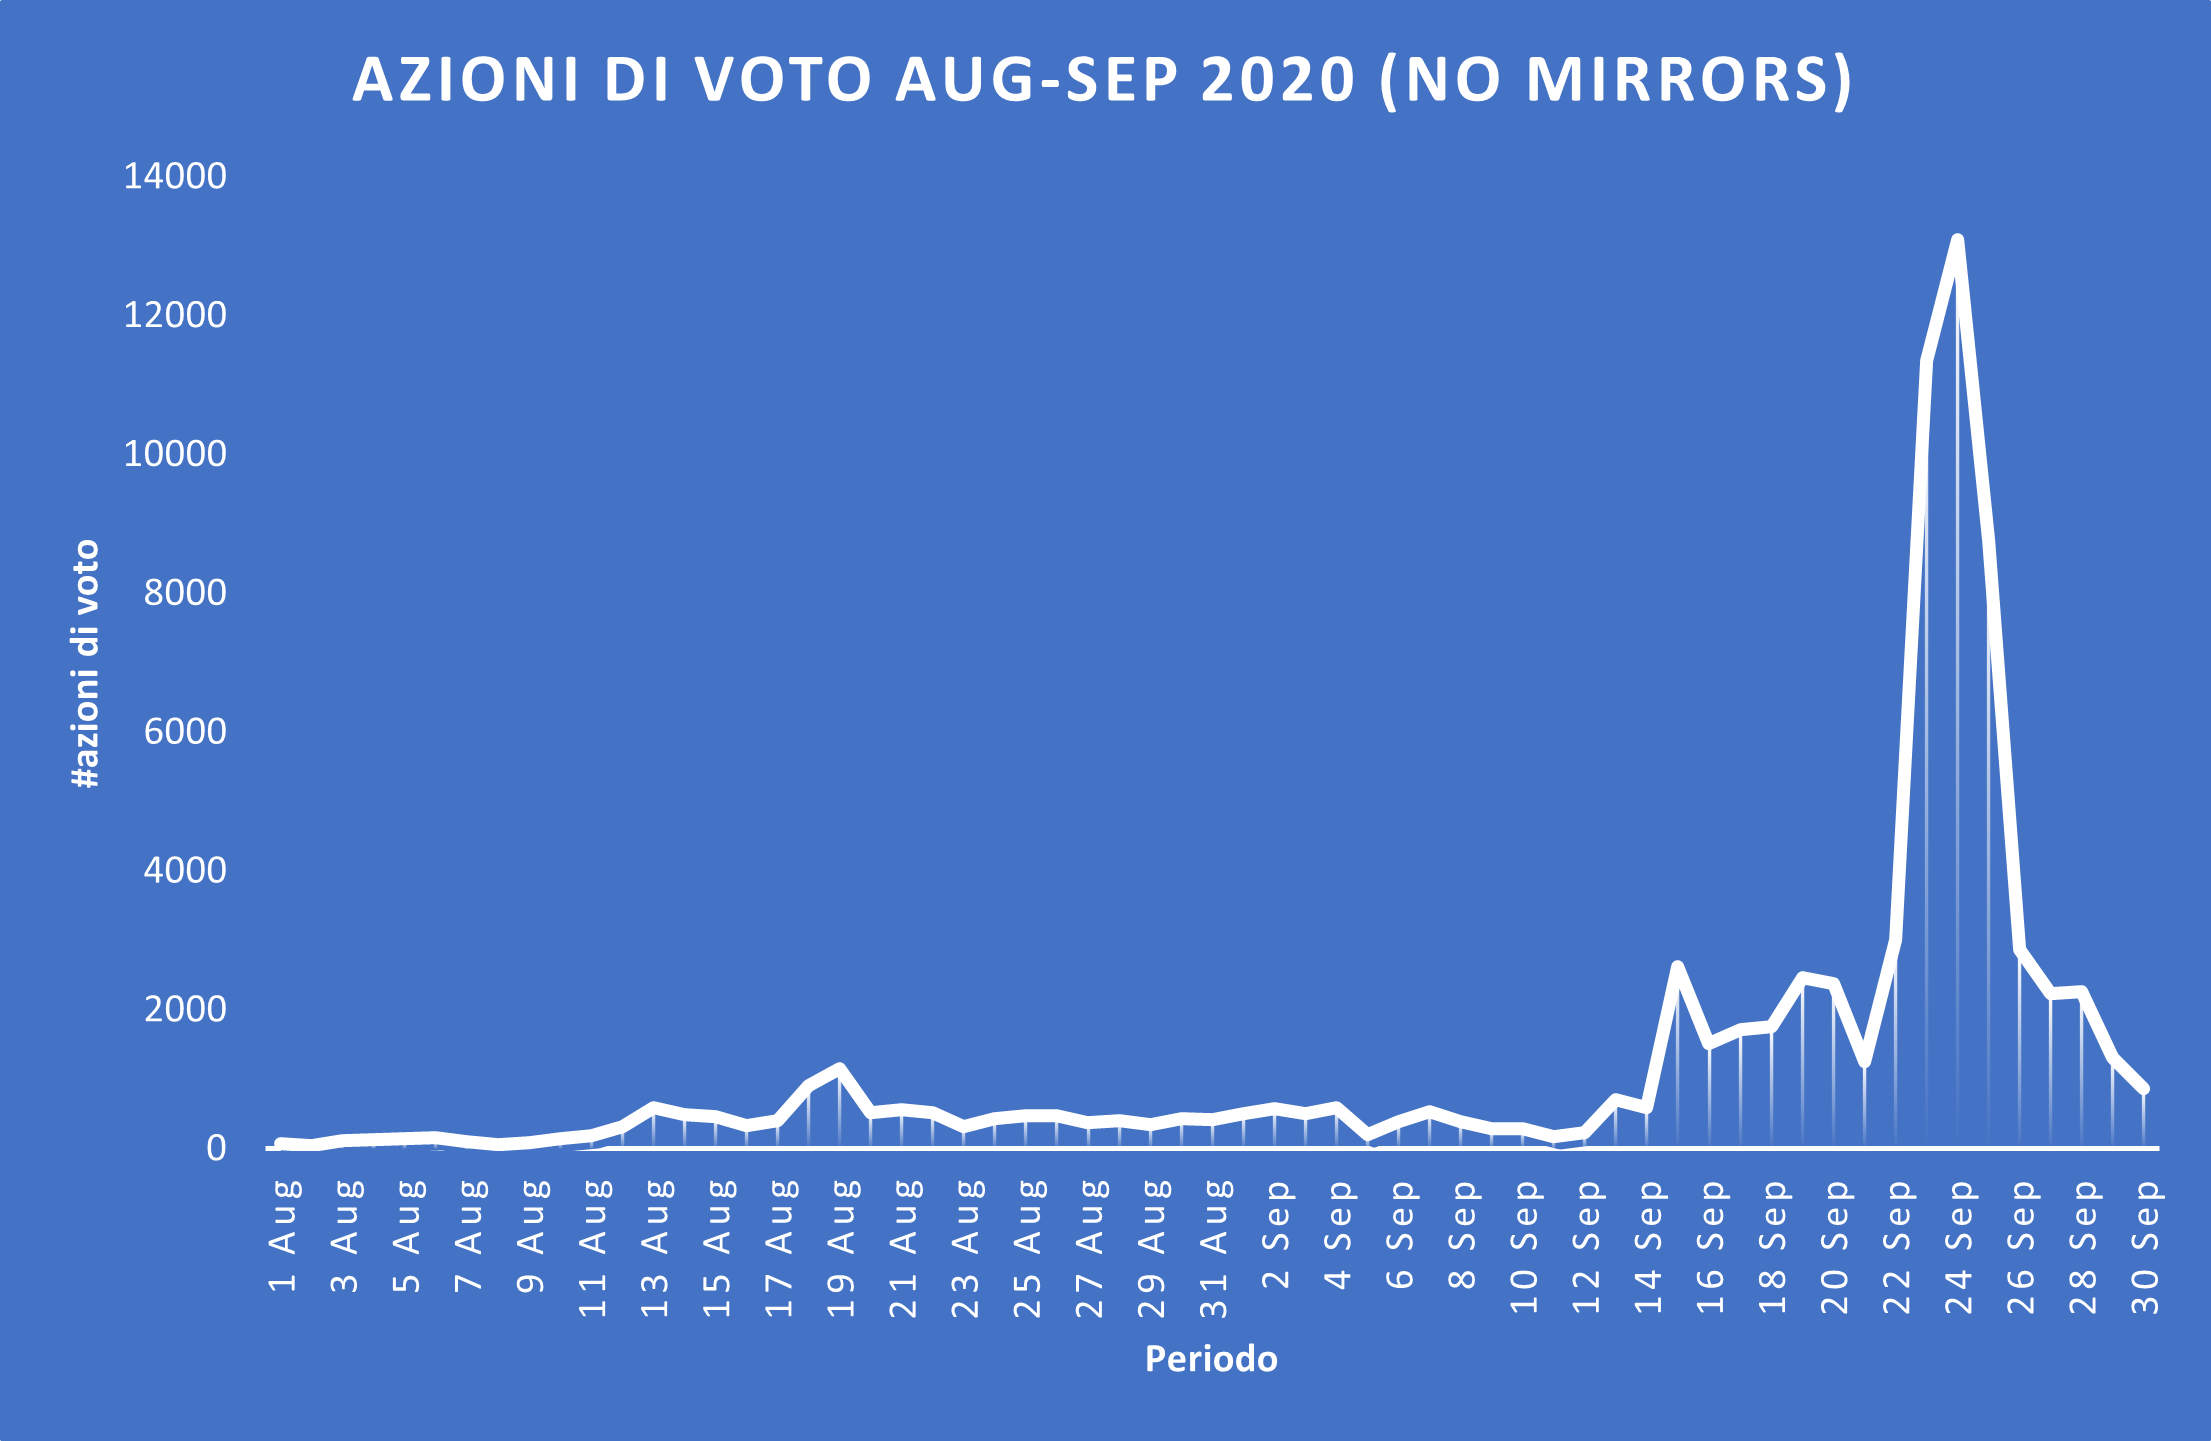
\includegraphics[width=.7\textwidth]{graphs/daily_azionivoto_nomirr.png}
    \caption{Distribuzione giornaliere delle azioni di voto, escluse quelle effettuate da account mirror}
    \label{fig: voting_daily_nomirr}
    
\end{figure}    
    %\vspace*{\floatstep}
\begin{figure}[t]
    \centering
    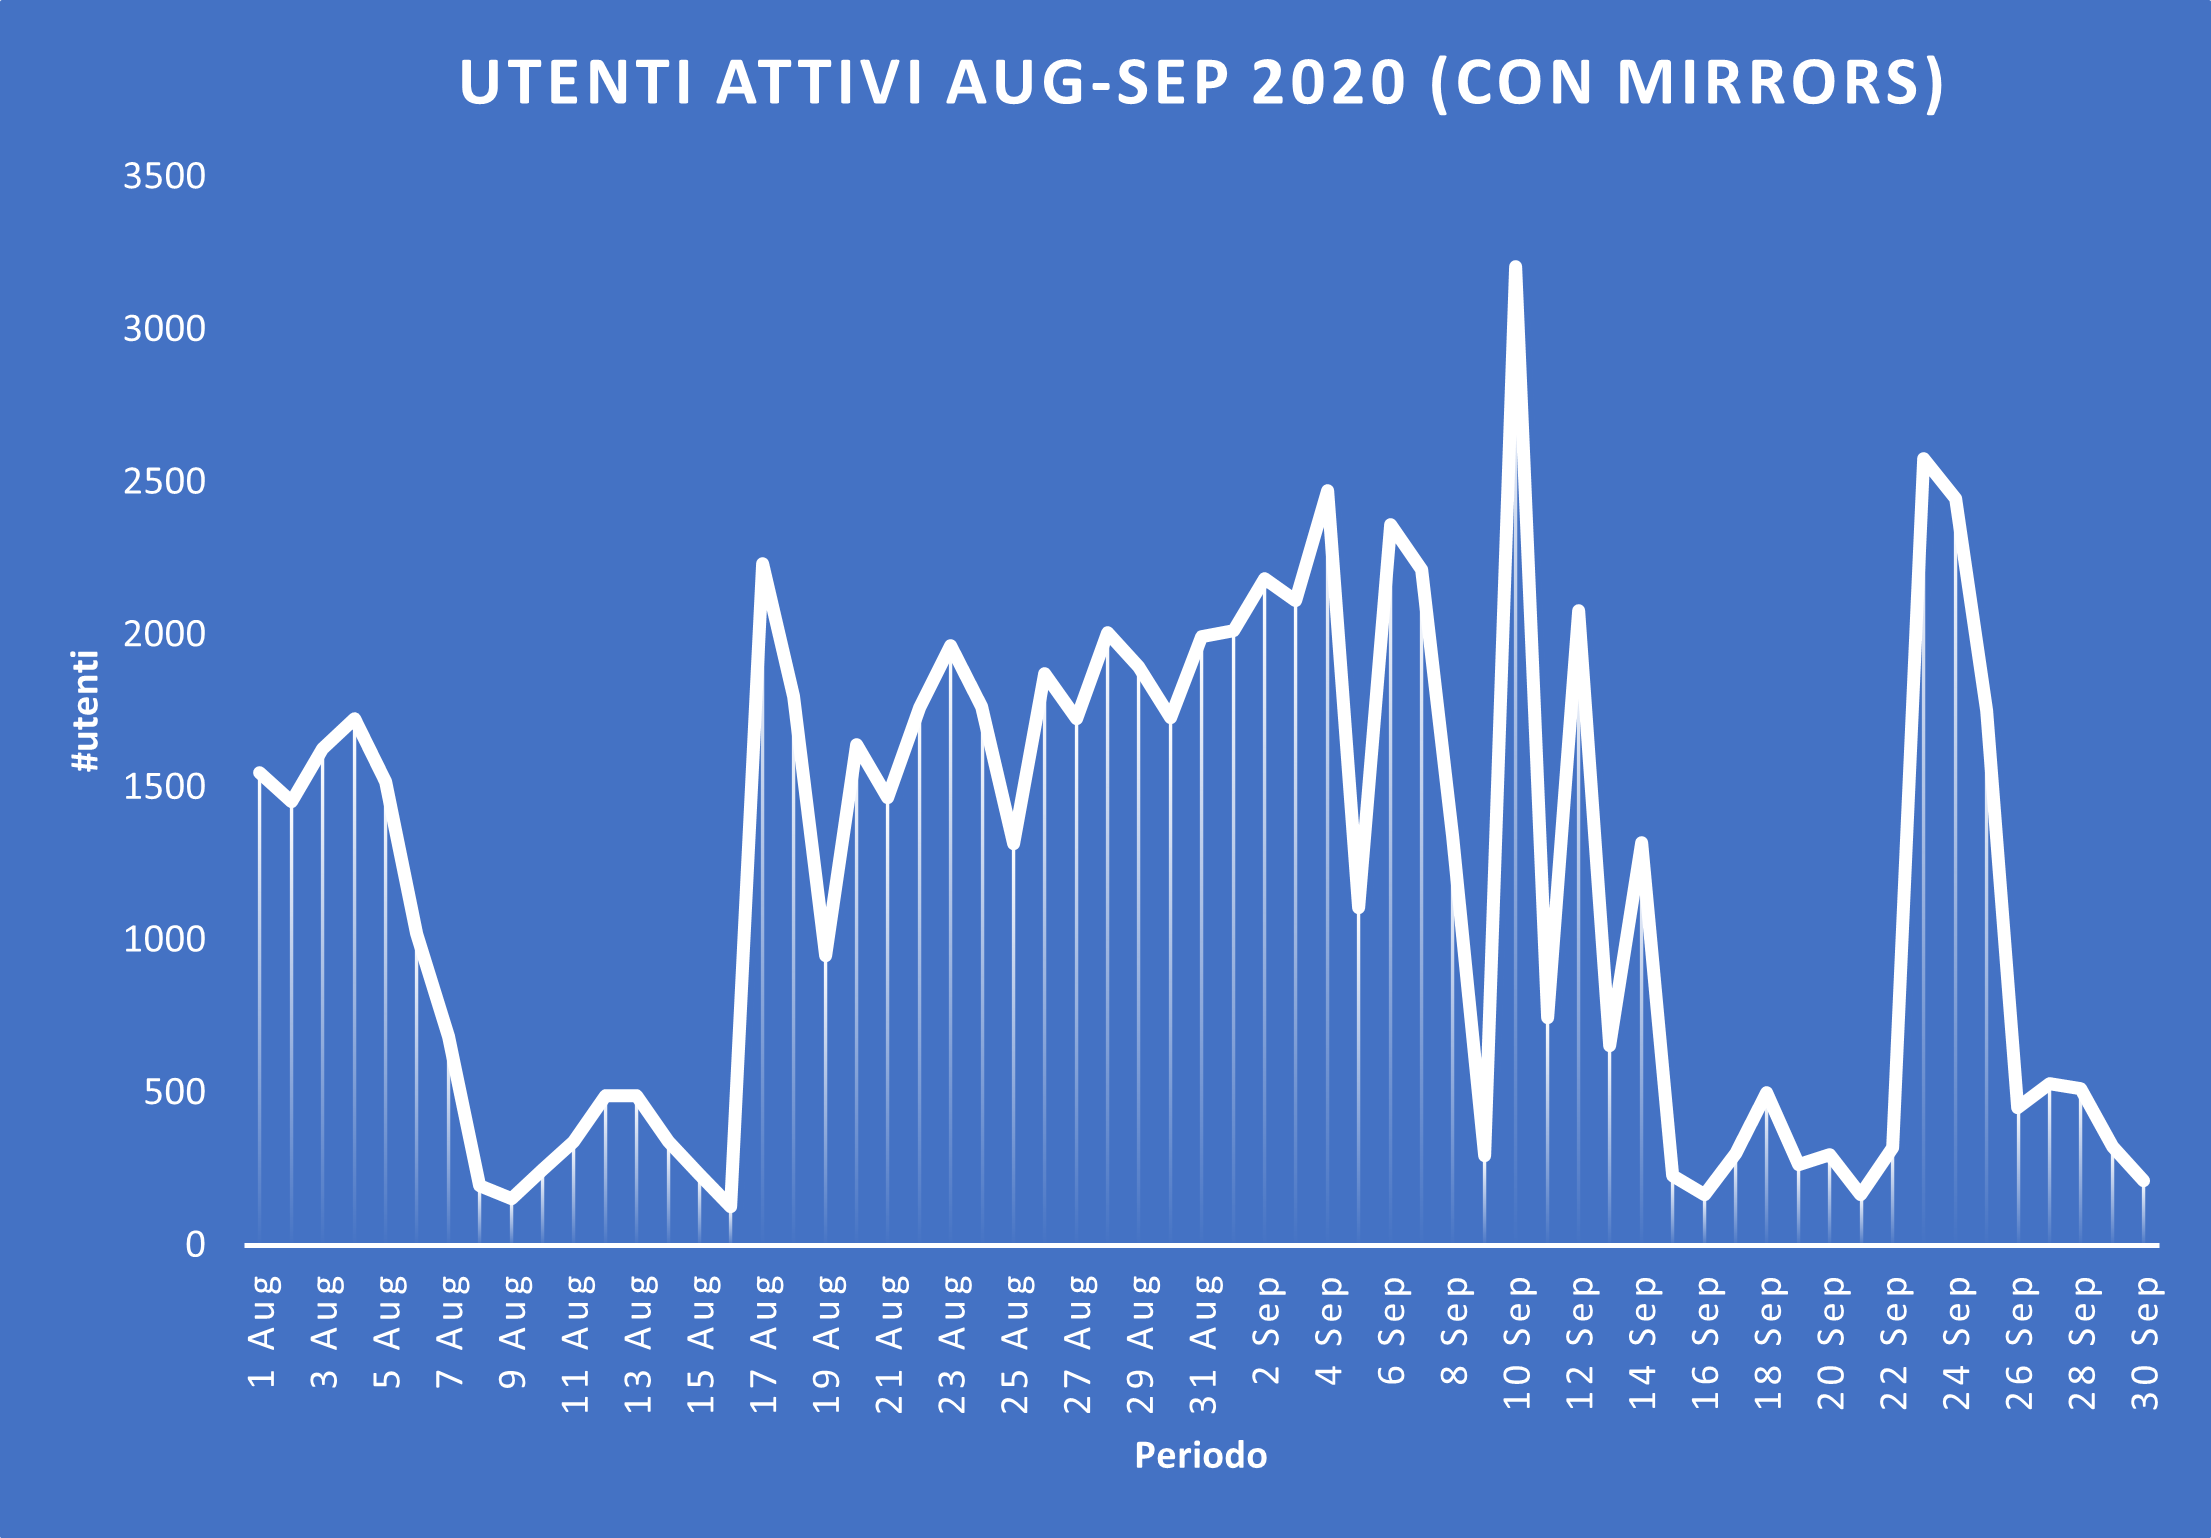
\includegraphics[width=.7\textwidth]{graphs/daily_attivi.png}
    \caption{Utenti attivi su base giornaliera includendo i Mirror}
    \label{fig: attivi_daily_conmirr}
\end{figure}


\begin{figure}[t]
    \centering
    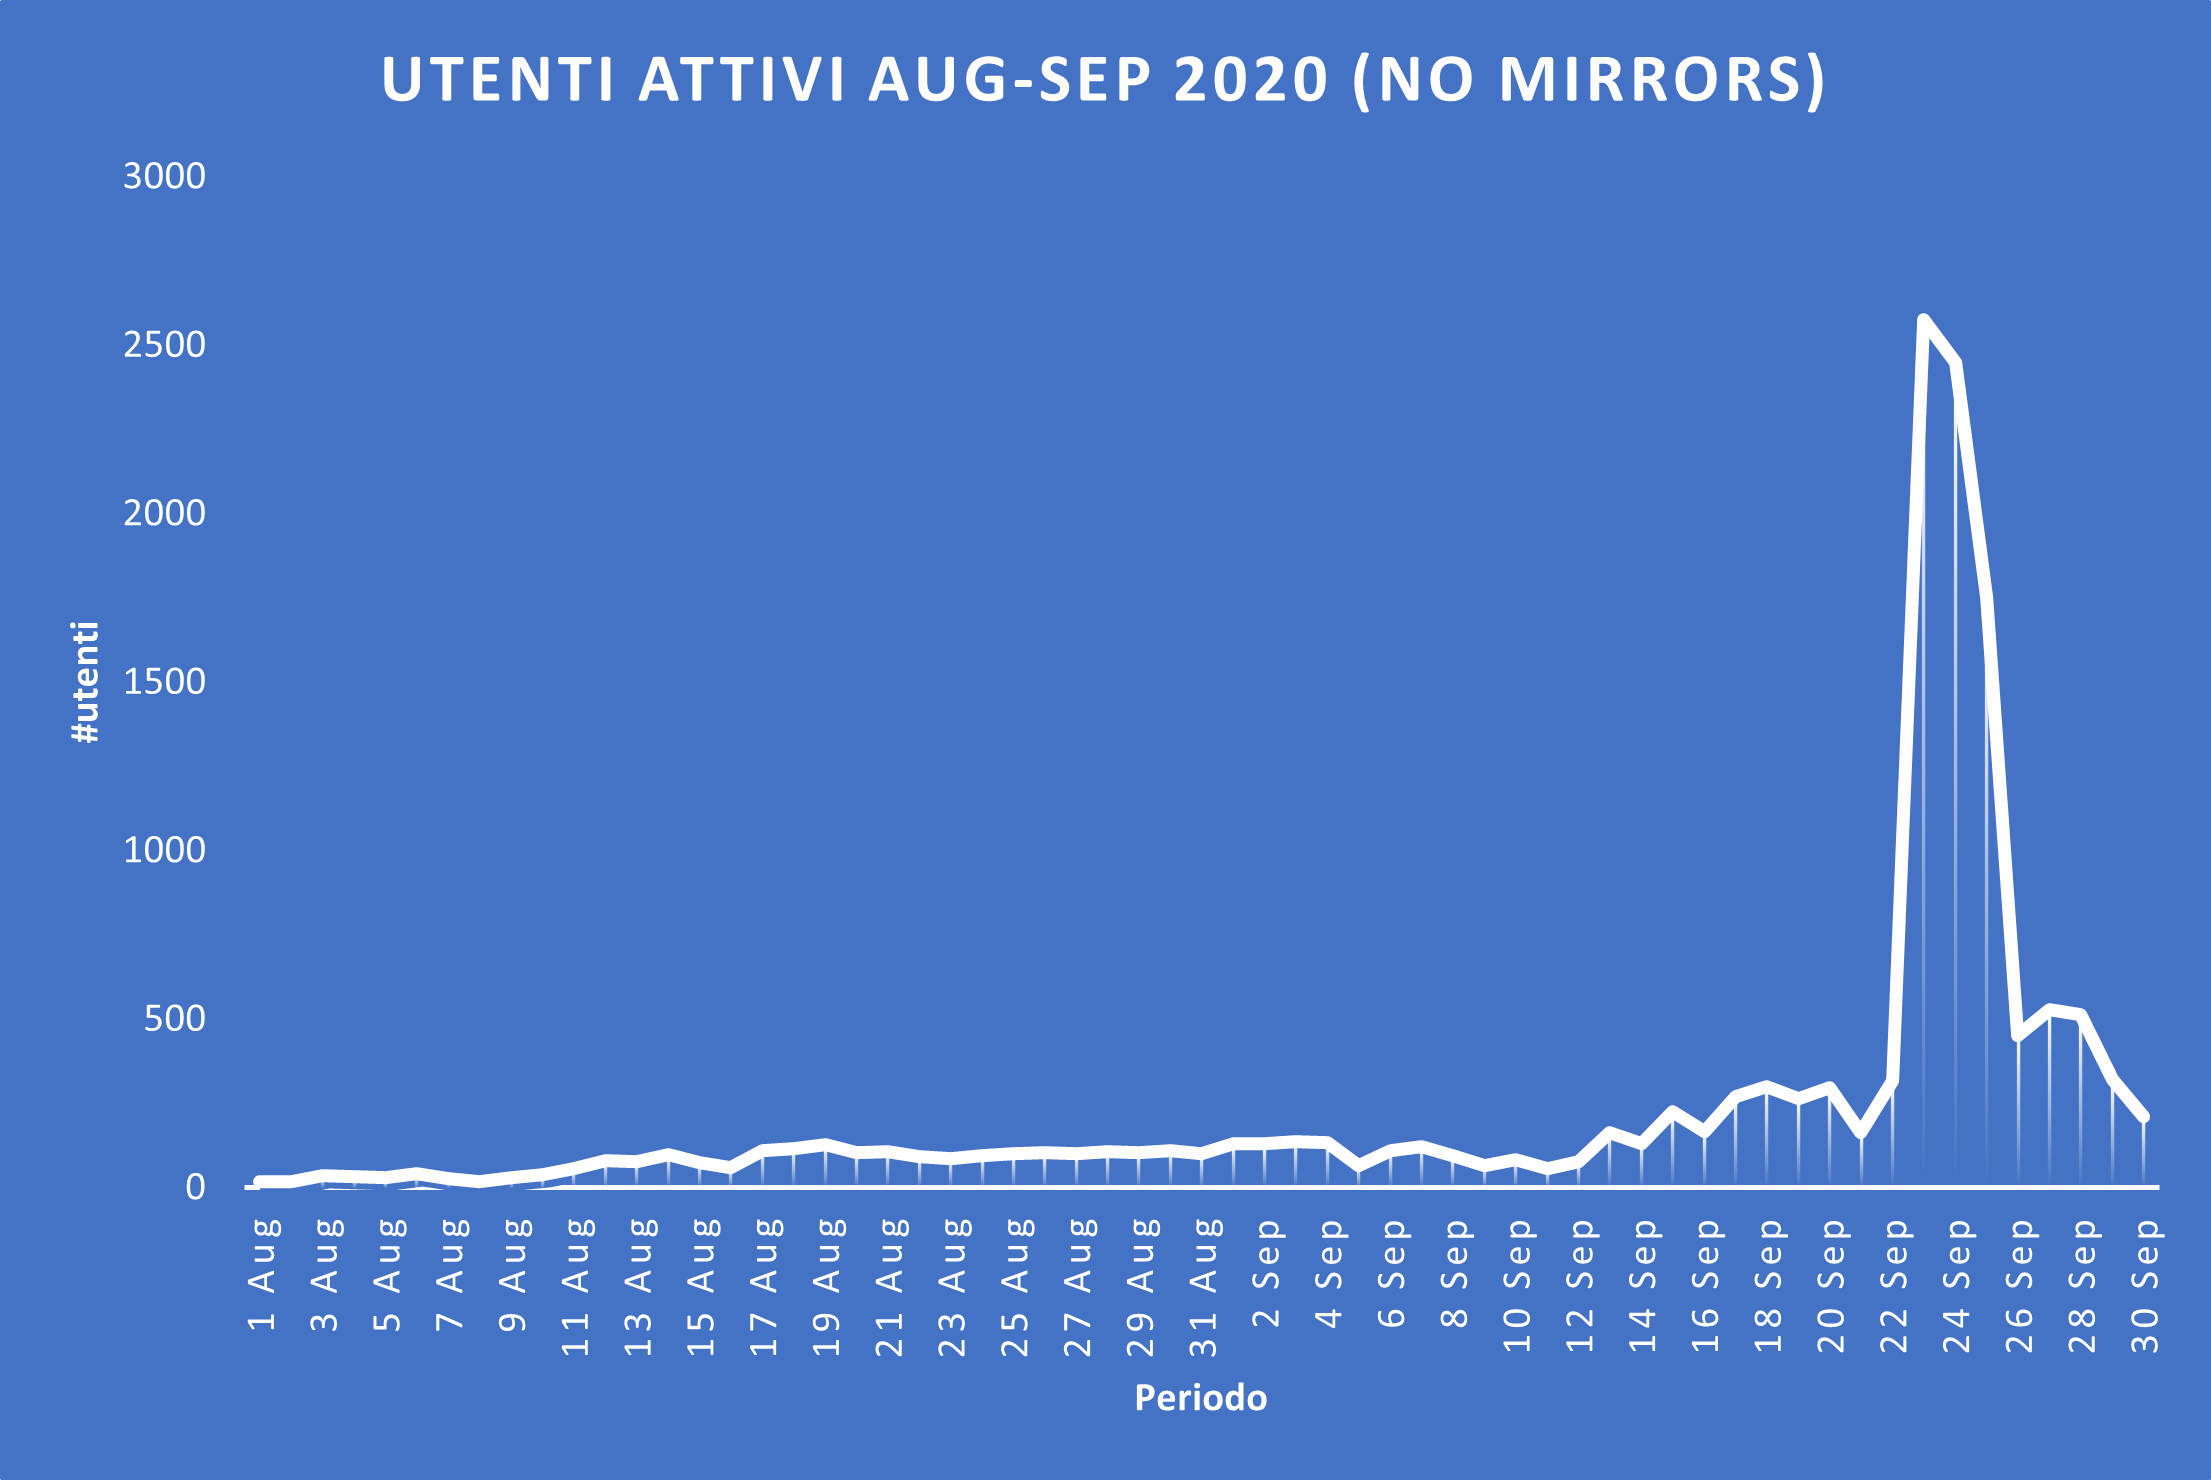
\includegraphics[width=.7\textwidth]{graphs/daily_attivi_nomirr.png}
    \caption{Utenti attivi su base giornaliera escludendo i Mirror}
    \label{fig: attivi_daily_nomirr}
\end{figure}

Si può notare un picco ricorrente, in data 23-24 Settembre 2020, in tutti e quattro gli ultimi grafici trattati e quindi indipendentemente dall'inclusione di account di sistema. Abbiamo tentato di individuare qualcosa che motivasse tale picco, purtroppo senza successo. Non sono stati individuati tweet sull'account ufficiale di Yup che promuovesse l'inizio di un qualche evento e non sono stati individuati nemmeno tweet che citassero Yup su account degli influencer maggiormente votati dalla community. Entrambe le eventualità avrebbero potuto causare l'incremento dell'attività voto. Il motivo di un picco del genere in quel periodo rimane pertanto sconosciuto.


% CAPITOLO: CONCLUSIONI E LAVORI FUTURI
\chapter{CONCLUSIONI E LAVORI FUTURI}
Nel mondo reale, i social networks e i social media giocano un ruolo fondamentale all'interno delle nostre vite. Il connubio tra social media e blockchain costituisce un’alternativa interessante, che, col tempo, potrebbe sostituire i meccanismi centralizzati tipici dei servizi Internet, ai quali si è più abituati, con meccaniche di funzionamento decentralizzate.
Lo scopo di questo tirocinio era quello di far luce sul funzionamento della dApp Yup, che risulta essere attualmente, una delle dApp sociali più utilizzate, con migliaia di utenti attivi al giorno\footnote{https://www.dapp.com/app/yup}. Ci siamo concentrati sull'analisi del protocollo, sul meccanismo di reward, ed infine sull'attività degli utenti. 
In ambito "social" è stata effettuata un'analisi della popolarità della piattaforma, evidenziando le azioni di creazione account, gli utenti attivi e la loro attività, la distribuzione dei voti per piattaforma e i profili più rilevanti su Yup. Spostandoci su un ambito più "economico" del protocollo ci siamo concentrati sull'utilizzo del servizio di Bridge e dei token posseduti e riscossi. Insieme costituiscono un'osservazione esaustiva dei profitti che gli utenti hanno tratto dall'utilizzo di Yup, sono infatti inclusi sia coloro che al momento mantengono i propri token su EOS, sia coloro che invece li hanno trasferiti su Ethereum.

Queste analisi hanno evidenziato delle particolarità interessanti del protocollo e dell'utilizzo che gli utenti fanno della piattaforma Yup. Tenendo conto del fatto che il codice dello Smart Contract non è pubblico e dell'assenza di documentazione relativa alle azioni che lo regolano, siamo riusciti, tramite l'analisi dei dati a nostra disposizione di capire la funzione di alcune azioni e a capire l'utilizzo tipico che ne fanno gli utenti.
In particolare, le nostre analisi hanno evidenziato l'esistenza di molti account, chiamati Mirror, non gestiti da umani ma che ripetono le azioni che alcune celebrità fanno sui propri account social.
Abbiamo inoltre scoperto che tra i contenuti più popolari spiccano quelli legati al mondo blockchain e investimenti in criptovalute e che gli stessi utenti Yup sfruttano un meccanismo, chiamato Bridge, per trasferire i propri fondi su Ethereum per poi utilizzarli come meglio credono.
Lo studio dell'attività degli utenti ha mostrato che in alcuni momenti lo smart contract di Yup su EOS non è stato in grado di sostenere il carico di lavoro, al punto che molti utenti si sono lamentati sui canali ufficiali che le ricompense per le loro attività non arrivano.

Abbiamo scaricato i dati relativi a Yup interfacciandosi con la blockchain EOS. Il dataset utilizzato per la fase di analisi prende in considerazione tutte le azioni presenti sullo smart contract principale (\textbf{yupyupyupyup}) dal \textit{15 Settembre 2018}, periodo di inizio della sua attività, fino al \textit{28 Febbraio 2021}. Abbiamo recuperato un numero di azioni pari a $23.567.430$. 
I dati degli utenti Yup sono stati reperiti in due modalità: conteggiando il numero di \textbf{createacct} sullo smart contract e scaricando il JSON contente tutti gli utenti utilizzando le API ufficiali. Abbiamo valutato come il numero di account presenti nel JSON è notevolmente superiore al numero di createacct, ciò significa che esistono account non generati tramite l'interazione con il protocollo. Abbiamo definito questi utenti Mirror e nelle analisi abbiamo valutato i risultati includendo ed escludendo tali account Mirror. In dettaglio, abbiamo appurato l'esistenza di \textit{16.484} account Yup, ma solo per \textit{11.045} di questi è stato possibile ritrovare una corrispondente azione di creazione account nel protocollo.



%\todo[inline]{Tutta questa introduzione deve essere estesa, andando ad integrare qui cosa si è fatto con l'analisi. Come un riassunto di tutto.}

%In ambito "social" è stata effettuata un'analisi della popolarità della piattaforma, evidenziando le azioni di creazione account e gli utenti attivi, e dell'attività degli utenti, evidenziando la distribuzione dei voti per piattaforma e profili a questa relativi. Spostandoci su un ambito più "economico" del protocollo ci siamo concentrati sull'utilizzo del servizio di Bridge e dei token posseduti e riscossi. Insieme costituiscono un'osservazione esaustiva dei profitti che gli utenti hanno tratto dall'utilizzo di Yup, sono infatti inclusi sia coloro che al momento mantengono i propri token su EOS, sia coloro che invece li hanno trasferiti su Ethereum.
%Nella maggior parte dei casi abbiamo sempre differenziato le analisi includendo e poi escludendo gli account Mirror, in modo da avere nel primo caso l'attività complessiva e nel secondo quella reale, visto che si considerano solo gli utenti effettivi.

%Durante la fase di analisi ci siamo concentrati principalmente nell'analisi economica e sociale della piattaforma, andando a valutare l'attività degli utenti. In dettaglio, abbiamo osservato vari aspetti del protocollo, tra cui l'utilizzo delle varie azioni, l'attività in termini di utenza, le varie piattaforme sociali coinvolte, ecc. Nel Capitolo \ref{analisi_marker}, sono riportate tutte le analisi effettuate e le considerazioni sui risultati ottenuti.
%\\
%\\
Considerando solo il periodo successivo alla conclusione della fase di Beta (\textit{6 Ottobre 2020 - Febbraio 2021}), risulta una media di circa \textit{700} utenti mensili socialmente attivi, ovvero che hanno effettuato almeno un'azione in ambito sociale in quel mese. Di questi è stato osservato un picco particolarmente alto nel mese di Settembre, specificamente tra il 23 e 24 del mese. Queste ultime considerazioni sono relative ai soli account non-Mirror, tuttavia nel capitolo dedicato alla fase di analisi tratteremo anche quelle che tengono in considerazione gli account di sistema.

Restando in ambito sociale abbiamo individuato contenuti votati appartenenti a 1.884 piattaforme diverse. Tra queste dominano tre delle quattro piattaforme integrate (in ordine Twitter, Youtube e Reddit), anche se è possibile notare una notevole presenza di quelle dedicate al commercio di NFT (come Rarible e SuperRare). Tra le piattaforme social, molti utenti mostrano grande interesse per i profili o gruppi che trattano argomenti legati al mondo cripto (Elon Musk e Binance su Twitter, fanatici ed esperti di criptomonete su Youtube). Caso particolare quello di Reddit, in cui troviamo, tra i più popolari, anche subreddit con materiale NSFW.

Spostandoci infine sull'ambito economico abbiamo analizzato il funzionamento del meccanismo di ricompense e la distribuzione dei token tra i vari utenti. Nel primo caso è stato notato come quelle destinate ai Creatori non vengano distribuite agli account Mirror corrispondenti bensì accumulate sull'account \textbf{yupcreators1}, apparentemente per una futura distribuzione quando più Creatori riscatteranno tali account o si iscriveranno alla piattaforma. Nel secondo è stato possibile osservare come gli utenti che hanno riscosso o possiedono più token siano, nella maggior parte dei casi, utenti che, oltre ad utilizzare il servizio, forniscono liquidità su Uniswap.
Abbiamo potuto inoltre constatare che i 3 utenti più ricchi della piattaforma posseggano oltre il 50\% dei token e che questo trend si sta estremizzando nel tempo.


\section{Lavori futuri}
Senza dubbio ci sono ancora molti aspetti della dApp Yup che richiedono un'analisi approfondita e che purtroppo non è stato possibile trattare in questa tesi. Di seguito elenchiamo alcuni possibili lavori futuri:

\begin{itemize}
    \item \textbf{Analizzare l'utilizzo delle risorse del protocollo (RAM, CPU, NET):} sarebbe interessante vedere il suo funzionamento in relazione alle risorse disponibili, visto che in alcuni casi è stato osservato un temporaneo blocco del servizio per via di una saturazione della RAM o CPU che ha causato probabilmente dei cali improvvisi di utilizzo della piattaforma, e nello specifico anche gli spostamenti di RAM, visto che può essere comprata e venduta.
    \item \textbf{Indagine su eventuale presenza di bot:} l'utilizzo di bot per effettuare dei voti è altamente probabile visto il grande incentivo economico che si ha dall'essere i primi a votare un contenuto e che in alcuni casi è facile prevedere quali contenuti saranno maggiormente votati. Questa analisi potrebbe essere condotta effettuando un controllo sul timestamp dell'azione nell'explorer, essendo in tempo reale, e quello del contenuto valutato utilizzando tecniche di analisi di time series.
    \item \textbf{Indagine account sospesi:} di tanto in tanto alcuni utenti vengono sospesi per aver violato determinate regole. A causa della sospensione questi utenti non possono esprimere voti e la loro Influenza viete settata a 0. Sarebbe interessante provare a capire quali siano le motivazioni che portano a questi ban temporanei e probabilmente sarebbe un buon inizio anche per l'analisi sui bot citata sopra.
    \item \textbf{Analisi sull'utilizzo dei token migrati su Ethereum:} pagando il Gas di Ethereum, e di conseguenza avendo accesso ai dati della blockchain, dovrebbe essere possibile rintracciare i token Yup che vengono trasferiti con il Bridge. Si potrebbe quindi scoprire come gli utenti spendono i token migrati su Ethereum, per esempio utilizzati per il mint di un NFT, scambiati per altre criptovalute su un exchange e così via.
    \item \textbf{Analisi transfer utente-utente:} essendo possibile inviare token ad un altro utente EOS senza commissioni, potrebbe essere interessante vedere, magari tramite l'utilizzo della teoria dei grafi, se ci sono utenti che periodicamente effettuano degli scambi tra loro. Un'indagine di questo tipo permetterebbe l'avanzamento di ipotesi sulla presenza di multi-account (una singola persona che gestisce più account Yup) o sull'utilizzo di tale funzionalità come pagamento tra individui.
\end{itemize}

% BIGLIOGRAFIA
\addcontentsline{toc}{chapter}{Bigliografia}
\printbibliography[title = Bigliografia]

% APPENDICE
\appendix
\setcounter{secnumdepth}{-1}
\chapter{Appendice A}
\label{appendix_marker}

\begin{table}[h!]
\centering
\begin{adjustbox}{width=0.6\textwidth}
\small
\begin{tabular}{|l|l|l|l|l|}
\hline
$\bullet$ alert & $\bullet$ amdeletevote & $\bullet$ broadcast & $\bullet$ buyram \\
\hline
$\bullet$ claimcurwd2 & $\bullet$ claimlqrwds & $\bullet$ cleanipfs & $\bullet$ cleanvvslg \\
\hline
$\bullet$ cleartables & $\bullet$ closeprv & $\bullet$ creapost & $\bullet$ create \\
\hline
$\bullet$ createcom & $\bullet$ createpostv2 & $\bullet$ createpostv3 & $\bullet$ createvote \\
\hline
$\bullet$ delacct & $\bullet$ delegatebw & $\bullet$ deleletebvote & $\bullet$ deleteipfs \\
\hline
$\bullet$ deletepost & $\bullet$ delvfollow & $\bullet$ delvpost & $\bullet$ delvvote \\
\hline
$\bullet$ deposit & $\bullet$ dice & $\bullet$ editvote & $\bullet$ fundcpuloan \\
\hline
$\bullet$ fundnetloan & $\bullet$ funstake & $\bullet$ funstakelq & $\bullet$ grab \\
\hline
$\bullet$ hashaccts & $\bullet$ hashowner & $\bullet$ hi & $\bullet$ i \\
\hline
$\bullet$ init & $\bullet$ initlqivl & $\bullet$ initupdcr & $\bullet$ initvotelc \\
\hline
$\bullet$ issue & $\bullet$ issueairdrop & $\bullet$ like & $\bullet$ linkauth \\
\hline
$\bullet$ logaddcom & $\bullet$ logaddfollow & $\bullet$ logaddpost & $\bullet$ logaddvote \\
\hline
$\bullet$ logbigint & $\bullet$ logdelpost & $\bullet$ logdelvote & $\bullet$ logintval \\
\hline
$\bullet$ logpostpool & $\bullet$ logupdfollow & $\bullet$ logupdvote & $\bullet$ logvoteupd \\
\hline
$\bullet$ m & $\bullet$ makeorder & $\bullet$ migrate & $\bullet$ migrateaccts \\
\hline
$\bullet$ migrateage & $\bullet$ migratepms2 & $\bullet$ migrateposts & $\bullet$ migrateposts4 \\
\hline
$\bullet$ migratevms & $\bullet$ migratevms2 & $\bullet$ mine & $\bullet$ move1 \\
\hline
$\bullet$ move2 & $\bullet$ newaccount & $\bullet$ news & $\bullet$ notify \\
\hline
$\bullet$ prcsslqivl2 & $\bullet$ processivl & $\bullet$ processivlv2 & $\bullet$ processprs2 \\
\hline
$\bullet$ push & $\bullet$ refreceipt & $\bullet$ refund & $\bullet$ regplayer \\
\hline
$\bullet$ rentcpu & $\bullet$ rentnet & $\bullet$ resetaccts & $\bullet$ resetckps \\
\hline
$\bullet$ resetckps2 & $\bullet$ resetckptl & $\bullet$ resetivllq & $\bullet$ resetprs \\
\hline
$\bullet$ rmckptl & $\bullet$ rmvm & $\bullet$ sayto & $\bullet$ selectpkg \\
\hline
$\bullet$ selldfs & $\bullet$ sellram & $\bullet$ sellusdd & $\bullet$ setabi \\
\hline
$\bullet$ setckp & $\bullet$ setcode & $\bullet$ setivldur & $\bullet$ setivllq \\
\hline
$\bullet$ setivllqsetivllstupd & $\bullet$ setivlpool & $\bullet$ setivlstats & $\bullet$ setivlstats2 \\
\hline
$\bullet$ setlqivlstat & $\bullet$ setlqivlstt2 & $\bullet$ setpostpool & $\bullet$ setpostpools \\
\hline
$\bullet$ settmstats & $\bullet$ settrstats & $\bullet$ setvm & $\bullet$ setvmcks \\
\hline
$\bullet$ setvmlikes & $\bullet$ setvotelc & $\bullet$ signup & $\bullet$ spaceinvader \\
\hline
$\bullet$ sportbet & $\bullet$ stake & $\bullet$ swap & $\bullet$ swaplog \\
\hline
$\bullet$ test & $\bullet$ transfer & $\bullet$ undelegatebw & $\bullet$ unstake \\
\hline
$\bullet$ updacc & $\bullet$ updagedeps & $\bullet$ updateauth & $\bullet$ updckps2 \\
\hline
$\bullet$ updcrrwds & $\bullet$ updlqivlstk & $\bullet$ updpost & $\bullet$ updvoteivls \\
\hline
$\bullet$ usage & $\bullet$ vinflratio & $\bullet$ voteproducer & $\bullet$ welcome \\
\hline
$\bullet$ winns & $\bullet$ withdraw & $\bullet$ xcleanup & $\bullet$ xcleanuprow \\
\hline
$\bullet$ xcommit & $\bullet$ xdcommit & $\bullet$ xsignal & $\bullet$ xwarmup \\
\hline
$\bullet$ xwarmuprow & $\bullet$ yell \\
\cline{1-2}
\end{tabular}
\end{adjustbox}
\caption{Azioni \textbf{non riconosciute}}
\label{tab: appendix_actions}
\end{table}


\end{document}
